% =====================================================================
%  Professioni 0 — Mindset e best practice: imparare a imparare
%  Fonte: trascrizione dell'incontro "Mindset e best practice" (AIV0)
%  della settimana dei Dev Days di inizio primo anno: un incontro
%  online su Zoom di circa un'ora e mezza, di pomeriggio (dalle 14:30
%  alle 16 circa), tenuto da Daniele Fusetto, direttore del corso di
%  narrative design e brand advisor dell'Accademia Italiana Videogiochi
%  (AIV). L'incontro è riservato a chi si è iscritto entro il 31 luglio
%  con la "Gamer Promo" o la "Dev Promo"; partecipano studenti di tutti
%  i corsi del primo anno. Slide condivise, molte domande a voce e in
%  chat prima, durante e dopo la parte frontale.
%  Pacchetti richiesti nel preambolo del libro:
%    \usepackage[utf8]{inputenc}, \usepackage{booktabs},
%    \usepackage{tikz} con
%    \usetikzlibrary{arrows.meta,positioning,calc,fit}
%    (le librerie vanno caricate nel preambolo, non nel capitolo)
%
%  Collocazione nel libro: parte "Alcune Professioni nel Mondo
%  Videoludico", come primo capitolo (3.1), prima di AIV1-AIV6.
%  Nel file principale del libro:
%
%    \part{Alcune Professioni nel Mondo Videoludico}
%    \renewcommand{\thechapter}{3.\arabic{chapter}}
%    \renewcommand{\theHchapter}{prof.\arabic{chapter}}
%    \setcounter{chapter}{0}
%    % =====================================================================
%  Professioni 0 — Mindset e best practice: imparare a imparare
%  Fonte: trascrizione dell'incontro "Mindset e best practice" (AIV0)
%  della settimana dei Dev Days di inizio primo anno: un incontro
%  online su Zoom di circa un'ora e mezza, di pomeriggio (dalle 14:30
%  alle 16 circa), tenuto da Daniele Fusetto, direttore del corso di
%  narrative design e brand advisor dell'Accademia Italiana Videogiochi
%  (AIV). L'incontro è riservato a chi si è iscritto entro il 31 luglio
%  con la "Gamer Promo" o la "Dev Promo"; partecipano studenti di tutti
%  i corsi del primo anno. Slide condivise, molte domande a voce e in
%  chat prima, durante e dopo la parte frontale.
%  Pacchetti richiesti nel preambolo del libro:
%    \usepackage[utf8]{inputenc}, \usepackage{booktabs},
%    \usepackage{tikz} con
%    \usetikzlibrary{arrows.meta,positioning,calc,fit}
%    (le librerie vanno caricate nel preambolo, non nel capitolo)
%
%  Collocazione nel libro: parte "Alcune Professioni nel Mondo
%  Videoludico", come primo capitolo (3.1), prima di AIV1-AIV6.
%  Nel file principale del libro:
%
%    \part{Alcune Professioni nel Mondo Videoludico}
%    \renewcommand{\thechapter}{3.\arabic{chapter}}
%    \renewcommand{\theHchapter}{prof.\arabic{chapter}}
%    \setcounter{chapter}{0}
%    % =====================================================================
%  Professioni 0 — Mindset e best practice: imparare a imparare
%  Fonte: trascrizione dell'incontro "Mindset e best practice" (AIV0)
%  della settimana dei Dev Days di inizio primo anno: un incontro
%  online su Zoom di circa un'ora e mezza, di pomeriggio (dalle 14:30
%  alle 16 circa), tenuto da Daniele Fusetto, direttore del corso di
%  narrative design e brand advisor dell'Accademia Italiana Videogiochi
%  (AIV). L'incontro è riservato a chi si è iscritto entro il 31 luglio
%  con la "Gamer Promo" o la "Dev Promo"; partecipano studenti di tutti
%  i corsi del primo anno. Slide condivise, molte domande a voce e in
%  chat prima, durante e dopo la parte frontale.
%  Pacchetti richiesti nel preambolo del libro:
%    \usepackage[utf8]{inputenc}, \usepackage{booktabs},
%    \usepackage{tikz} con
%    \usetikzlibrary{arrows.meta,positioning,calc,fit}
%    (le librerie vanno caricate nel preambolo, non nel capitolo)
%
%  Collocazione nel libro: parte "Alcune Professioni nel Mondo
%  Videoludico", come primo capitolo (3.1), prima di AIV1-AIV6.
%  Nel file principale del libro:
%
%    \part{Alcune Professioni nel Mondo Videoludico}
%    \renewcommand{\thechapter}{3.\arabic{chapter}}
%    \renewcommand{\theHchapter}{prof.\arabic{chapter}}
%    \setcounter{chapter}{0}
%    % =====================================================================
%  Professioni 0 — Mindset e best practice: imparare a imparare
%  Fonte: trascrizione dell'incontro "Mindset e best practice" (AIV0)
%  della settimana dei Dev Days di inizio primo anno: un incontro
%  online su Zoom di circa un'ora e mezza, di pomeriggio (dalle 14:30
%  alle 16 circa), tenuto da Daniele Fusetto, direttore del corso di
%  narrative design e brand advisor dell'Accademia Italiana Videogiochi
%  (AIV). L'incontro è riservato a chi si è iscritto entro il 31 luglio
%  con la "Gamer Promo" o la "Dev Promo"; partecipano studenti di tutti
%  i corsi del primo anno. Slide condivise, molte domande a voce e in
%  chat prima, durante e dopo la parte frontale.
%  Pacchetti richiesti nel preambolo del libro:
%    \usepackage[utf8]{inputenc}, \usepackage{booktabs},
%    \usepackage{tikz} con
%    \usetikzlibrary{arrows.meta,positioning,calc,fit}
%    (le librerie vanno caricate nel preambolo, non nel capitolo)
%
%  Collocazione nel libro: parte "Alcune Professioni nel Mondo
%  Videoludico", come primo capitolo (3.1), prima di AIV1-AIV6.
%  Nel file principale del libro:
%
%    \part{Alcune Professioni nel Mondo Videoludico}
%    \renewcommand{\thechapter}{3.\arabic{chapter}}
%    \renewcommand{\theHchapter}{prof.\arabic{chapter}}
%    \setcounter{chapter}{0}
%    \input{Professioni/AIV0_mindset_e_best_practice}
%    \input{Professioni/AIV1_dev_days_e_metodo_aiv}
%    ...
%
%  Tutte le etichette di questo capitolo hanno il prefisso "p0:"
%  (p0:cap:..., p0:sec:..., p0:fig:..., p0:tab:...). Il capitolo
%  contiene alcuni rimandi al capitolo AIV1 (prefisso "p1:"), che
%  racconta l'incontro di apertura della stessa settimana.
%  Le figure sono ricostruzioni schematiche di quanto il relatore spiega
%  a voce e con le slide, non copie delle slide.
% =====================================================================

\chapter[Mindset e best practice]{Mindset e best practice: imparare a
imparare}
\label{p0:cap:mindset}

Questo capitolo raccoglie un incontro che, a rigore, non riguarda nessuna
professione in particolare, ma tutte: è la lezione su \textbf{mindset e best
practice} che l'Accademia Italiana Videogiochi (d'ora in poi \textbf{AIV})
dedica, nella prima settimana del primo anno, al \textbf{metodo di studio}.
Il tema è come si \emph{impara}: la differenza fra studiare e apprendere, i
meccanismi della memoria, le tecniche che aiutano a trasformare ciò che si
ascolta a lezione in conoscenza duratura, e due strumenti di
\textbf{problem solving} (la piramide del feedback e la tecnica
dell'iceberg) che servono tanto a risolvere un compito quanto a gestire un
playtest o un collega. Lo si mette in apertura di questa parte del libro
perché è la base su cui poggia tutto il resto: i capitoli successivi
descrivono che cosa fanno game designer, narrative designer, animatori,
programmatori e 3D artist, questo descrive come si diventa uno di loro.

A tenere l'incontro è \textbf{Daniele Fusetto}, direttore del corso di
narrative design e \emph{brand advisor} di AIV, lo stesso che il lunedì
mattina ha aperto la settimana dei \emph{Dev Days} insieme al direttore
della didattica (capitolo~\ref{p1:cap:devdays}). L'incontro non è per
tutti: è riservato a chi si è iscritto entro il 31 luglio con la
``\emph{Gamer Promo}'' o la ``\emph{Dev Promo}'', e lo si annuncia così fin
dal lunedì\footnote{Nel capitolo~\ref{p1:cap:devdays} il relatore lo
presenta come ``un incontro di mindset best practice dove andiamo a vedere
le pratiche migliori per imparare e per apprendere correttamente durante
l'anno scolastico''. Le stesse promozioni danno diritto anche a un'ora di
\emph{mentorship} individuale con un docente.}. Si svolge \textbf{online},
su Zoom, il martedì pomeriggio: l'inizio era previsto ``più o meno alle due
e mezza'' e la durata è di circa un'ora e mezza (``un'ora e mezza ce la
caviamo''). Il relatore arriva con qualche minuto di ritardo (``devo finire
delle altre attività \ldots\ intanto fatevi un caffè'') e, mentre si
aspettano gli altri, risponde a parecchie domande; la parte frontale
comincia solo dopo.

Tre avvertenze di lettura. La prima: la trascrizione è automatica e, nei
minuti di attesa, registra lunghi brani privi di senso (frasi ripetute
decine di volte, che non hanno nulla a che vedere con l'incontro); il
capitolo li ignora. La seconda: molti nomi propri e termini tecnici sono
storpiati (``Arial Engine'' o ``Arreal'' per Unreal Engine, ``Zygarnik''
per Zeigarnik, ``Ebinghausen'' per Ebbinghaus, ``Aeros Journey'' per
\emph{Hero's Journey}, ``Non H. Takeuchi'' per Nonaka e Takeuchi); dove la
ricostruzione è sicura il capitolo usa la forma corretta, altrimenti lo
segnala in nota. La terza: il relatore dichiara apertamente di non essere
uno scienziato (``non sono uno scienziato neurocognitivo, non ho studiato
medicina, quindi vi insegno delle cose da neofita'') e di basare gran parte
della parte neurocognitiva su un corso online gratuito; dove le sue
affermazioni si discostano dalla letteratura scientifica corrente, il
capitolo lo segnala in nota senza correggere il testo.

Quanto alla data, l'incontro si colloca con ogni probabilità
\textbf{martedì 6 ottobre 2026}\footnote{La data non è mai detta. La si
ricava dagli altri incontri della stessa settimana: il lunedì (``lunedì
mattina'', capitolo~\ref{p1:cap:devdays}) si è tenuta l'apertura; la
mattina stessa (``stamattina'') si è tenuta la presentazione del corso di
narrative design, al termine della quale il relatore dà appuntamento ``oggi
pomeriggio alle due e mezza''; le lezioni di narrative cominciano ``venerdì
9 ottobre'' e quelle degli altri corsi il 19 ottobre. Nel 2026 il 9 ottobre
è un venerdì. È una deduzione, non un'informazione esplicita.}.

Il percorso del capitolo segue quello dell'incontro:
\begin{enumerate}
  \item le domande nell'attesa: computer, schede grafiche, versione di
        Unreal, intelligenza artificiale (sezione~\ref{p0:sec:attesa});
  \item il programma e le fonti (sezione~\ref{p0:sec:programma});
  \item un ripasso del metodo AIV (sezione~\ref{p0:sec:metodo});
  \item la distinzione fra \textbf{studio} e \textbf{apprendimento}
        (sezione~\ref{p0:sec:studio});
  \item le basi dello studio: il paradosso delle fotocopie, i canali di
        apprendimento, dati, informazioni e conoscenza
        (sezioni da~\ref{p0:sec:basi} a~\ref{p0:sec:dati});
  \item tre modelli: la spirale della conoscenza, il ciclo della
        competenza, le curve di apprendimento e di oblio, e un bias,
        l'effetto Dunning-Kruger (sezioni da~\ref{p0:sec:spirale}
        a~\ref{p0:sec:curve});
  \item \textbf{mindset}, \textbf{skill set} e \textbf{tool set}
        (sezione~\ref{p0:sec:set});
  \item cenni di \textbf{neurocognitività}: memoria di lavoro e memoria a
        lungo termine, \emph{chunking}, consolidamento, modalità
        focalizzata e diffusa, limiti della memoria (sezioni
        da~\ref{p0:sec:memoria} a~\ref{p0:sec:limiti});
  \item la piramide della conoscenza e il modo in cui AIV prova a dare
        esperienza (sezione~\ref{p0:sec:piramide});
  \item le \textbf{tecniche di apprendimento}
        (sezione~\ref{p0:sec:tecniche});
  \item il \textbf{problem solving}: piramide del feedback e tecnica
        dell'iceberg (sezioni~\ref{p0:sec:feedback} e~\ref{p0:sec:iceberg});
  \item le domande finali (sezione~\ref{p0:sec:domande}).
\end{enumerate}

% ---------------------------------------------------------------------
\section{Nell'attesa: domande su computer, Unreal e intelligenza
artificiale}
\label{p0:sec:attesa}

Il relatore entra, chiede qualche minuto e invita a scrivere in chat il
corso che si frequenterà, ``mentre aspettiamo''. Arrivano game design
(molti), programming, narrative design, 3D art. Intanto, ``giusto per non
avere questo quart silence'', i partecipanti cominciano a fare domande;
il relatore le accoglie volentieri, ``anche sulla scuola, sull'accademia''.

\subsection{Quanta RAM?}

Uno studente di game programming ha un portatile con \textbf{16 GB di RAM}
e chiede se convenga aggiungerne altri 16. La risposta: sì, è importante,
``magari non subito'', ma la tendenza è andare verso i \textbf{32 GB}. Il
relatore ne ha ``già presi in previsione 64, ma forse 64 è già troppo''.
Se non ci sono i mezzi subito, ``per Natale, magari, o con\ldots\
festività, compleanno''. E soprattutto: \textbf{aspettare l'inizio del
corso} (il 19 ottobre, per programming) e chiedere ai docenti del corso,
che sapranno consigliare meglio; un docente di programmazione, Alessandro
Pregnolato, conosce per esempio servizi, anche gratuiti, per
\textbf{affittare un computer potente in cloud} per un'ora, una soluzione
``che puoi usare nel mentre''. La stessa domanda sulla RAM era emersa anche
il lunedì (capitolo~\ref{p1:cap:devdays}), con la stessa risposta.

\subsection{Il lavoro e l'intelligenza artificiale}

Marco chiede se l'intelligenza artificiale, che ``sta facendo quasi
tutto'' e ``farà sempre meglio'', avrà conseguenze su questo tipo di lavoro.
La risposta del relatore è netta: anzitutto, l'idea che l'IA stia facendo
tutto ``non è reale, almeno nella mia esperienza''. Lui lavora ancora
``senza problemi'', con clienti, e così i programmatori. C'è stata ``fino a
qualche tempo fa una spinta'' a usarla per accelerare e per essere più
\emph{proficient}, ma ``è più complesso di così e le aziende iniziano ad
accorgersene''.

Un segnale lo vede proprio in AIV: quest'anno c'è stata ``una flessione sul
numero di programmatori iscritti'', perché ``tutti dicono: vabbè, ormai ce
li ha'' l'IA. Ma il relatore, che nella vita fa anche siti web, racconta i
``drammi'' che vede in chi programma siti con l'IA: funziona, ``sì, ho
capito, ma ti sei aperto il sito a malware''. Per usare l'IA ``devi sapere
di cosa parli'': quante volte Claude gli restituisce JavaScript, CSS o HTML
``che non ha alcun tipo di senso''. Un conto è usarla per farsi scrivere la
base di qualcosa che si saprebbe fare a mano, dando indicazioni; un altro è
quando si deve ``strutturare altro''. Ultimamente fa meno siti, per scelta
(``non voglio gestire clienti boomer''), ma vede ancora molta gente
convinta che ``con due trick si fa il sito'', che poi torna da lui perché
``non vende niente''.

Questo non vuol dire che l'IA vada ignorata: ``non dovete pensare che\ldots\
non dovete usarla, non dovete esplorarla''. Il rischio vero, come si diceva
anche ``stamattina'', è che alle persone \textbf{venga chiesto di più}: se
l'IA fa la base, si pretenderà che il programmatore faccia ``cose
avanzatissime''. Ma c'è qualcosa che l'IA non potrà mai sostituire:
\textbf{il pensiero}, perché ``il prompt viene dall'umano''. E non vale
l'obiezione ``faccio scrivere il prompt all'IA'': ``non funziona''.

\subsection{Gli iscritti che mancano}

Qualcuno nota che sono pochi: il lunedì si era detto che il primo anno
dovrebbe contare un centinaio di iscritti, mentre ``ieri mattina ce n'erano
30, stamattina ce n'erano 20''. Il relatore conferma, con un certo
disappunto: le classi ci sono, ma le persone non si presentano. Accenna a
``IA, TikTok, i social'' (``io non sono cospirazionista, lo ripeto, ma
abbiamo lasciato la tecnologia troppo in capo alle nostre vite''). Di
solito AIV conta \textbf{tra i 260 e i 300 iscritti totali}, di tutti gli
anni e di tutti i corsi, ``poi dipende da anno ad anno''.

\subsection{Quale scheda grafica per Unreal?}

Uno studente di game design vuole comprare un computer nuovo per dicembre,
``dato che avrò a che fare con Unreal Engine'', e chiede su quali schede
grafiche puntare, dato che sui 32 GB di RAM è ormai chiaro. È un argomento
``molto tricky'', che verrà ripreso nei corsi, ma in generale il relatore
consiglia di \textbf{stare su una serie 40} (di NVIDIA GeForce, si
intende). Il motivo: lui ne ha attualmente una della serie 50, ma ``noi
sviluppiamo giochi ancora oggi per'' schede molto più vecchie\footnote{La
trascrizione dice ``per una serie 10, 80, 20 e qualcosa'': il senso è che
si sviluppa ancora per schede di generazioni precedenti (serie 10, 20 e
simili, come una GTX 1080), non che il relatore ne indichi una precisa.},
perché ci sono persone che non possono permettersi macchine potenti. Non si
è quindi obbligati a prendere ``una di quelle super GeForce'': una serie 30
o una serie 40 ``bella solida'' va ``assolutamente bene''.

Il criterio decisivo è un altro: \textbf{fa fede l'apertura di Unreal
Engine}. Quando cominceranno le lezioni, ci sarà una lezione dedicata (``di
programmazione'') in cui verrà comunicata la versione di Unreal che si
userà, perché ogni anno i docenti si mettono d'accordo, dato che ogni anno
esce una versione nuova. Bisognerà andare sul sito, guardare le specifiche
richieste e verificare che il proprio computer ``apra Unreal''. Chi non
riuscisse a dotarsi di una macchina adeguata chieda ai docenti.

\subsection{Unreal 6, i Blueprint e Verse}

Qualcuno chiede se verrà usato Unreal Engine 6. Il relatore spiega la
politica di AIV: si evita di usare versioni di Unreal ``che non sono
completamente testate, implementate e usate nell'industria''. Secondo il
relatore, a gennaio dovrebbe arrivare Unreal 6, almeno in una versione
iniziale o di fine beta; quest'anno si è usata ancora la 5.8, ``perché era
la più solida''\footnote{Così nella trascrizione. Il relatore cita, come
versioni in uso nei progetti, ``5, 5.4, 5.6 \ldots\ 5.8, Unreal 6'', e dice
di usare personalmente la 5.6. Le informazioni su date e versioni sono
quelle riferite dal relatore nell'autunno 2026 e non sono state
verificate.}. Nell'industria, del resto, i progetti usano la versione di
Unreal disponibile al momento in cui partono e passano a una nuova
\textbf{solo se il passaggio non significa rifare tutto da zero}: ci si deve
aspettare di vedere ancora progetti in Unreal 5, 5.4, 5.6, 5.8 (lui usa la
5.6).

Unreal 6 verrà adottato solo quando ne saranno confermate le specifiche.
Secondo il relatore, l'annuncio ha lasciato ``basiti'' molti sviluppatori
perché Epic avrebbe detto di voler \textbf{discontinuare nel tempo i
Blueprint}, salvo poi correggersi (``non li discontinueremo subito''), e di
voler passare da C++ a \textbf{Verse}, ``un linguaggio abbastanza semplice e
complesso, però un linguaggio diverso''\footnote{È la ricostruzione del
relatore, riportata qui com'è; il capitolo non ha modo di verificare i
dettagli dell'annuncio. Verse è il linguaggio di scripting introdotto da
Epic con l'editor di Fortnite (UEFN).}. AIV lo userà solo quando l'industria
lo implementerà nei suoi giochi; se l'industria deciderà di non usare
Unreal 6, se ne riparlerà l'anno successivo. Per ora, osserva il relatore,
gli unici giochi annunciati con Unreal 6 sono quelli di studi che hanno una
partnership e investimenti legati a Epic, ``giustamente''.

Un altro studente racconta di avere un computer fisso con una scheda serie
40 e di lasciarlo acceso per usarlo a distanza con AnyDesk dal portatile.
``Bravissimo'', commenta il relatore: è un'ottima soluzione, ``soprattutto
se hai una wifi a bassa latenza''.

% ---------------------------------------------------------------------
\section{Il programma e le fonti}
\label{p0:sec:programma}

Dopo qualche problema di condivisione dello schermo (``io vedo tutto
nero''; ``è Zoom'') il relatore presenta il programma:
\begin{enumerate}
  \item un \textbf{recap del metodo di AIV} visto il lunedì mattina;
  \item la distinzione fra \textbf{studio} e \textbf{apprendimento};
  \item \textbf{cenni di neurocognitività};
  \item le \textbf{tecniche di apprendimento};
  \item in fondo, non segnata nell'indice delle slide, una breve parte sul
        \textbf{problem solving}.
\end{enumerate}
Il giovedì mattina, poi, con tutti gli altri colleghi del primo anno, si
farà l'incontro sulla \textbf{comprensione del testo}
(capitolo~\ref{pt:cap:comprensione})\footnote{Nella
trascrizione il relatore dice ``lunedì e giovedì mattina'', ma l'incontro
sulla comprensione del testo, come annunciato il lunedì
(capitolo~\ref{p1:cap:devdays}), è uno solo, il giovedì mattina; il
``lunedì'' si riferisce con ogni probabilità all'apertura della settimana.}.

\subsection{I libri e le playlist}

Una slide mostra i libri su cui si basano le slide, libri che il relatore
ha usato negli anni anche per narrative design, dove sono
``importantissimi''. Non vanno presi né letti tutti subito, ma sono molto
interessanti anche per il game designer: raccontano \textbf{come i
giocatori usano il cervello}, come le persone usano il cervello. Le
neuroscienze sono ``un ambito molto interessante'' per capire che effetti
hanno certe scelte sulla mente del giocatore.

Due link, cliccabili nelle slide, portano a due \textbf{playlist}: una,
\emph{Learning Curve}, fatta dal relatore; l'altra legata a \emph{Learning
How to Learn}, il corso di \textbf{Barbara Oakley e Terrence
Sejnowski}\footnote{La trascrizione storpia il nome in ``Terence
Egnoschi'' e, più avanti, ``Terence Semyoski''.}, i due professori su cui è
basata ``gran parte'' delle slide. Il loro corso \emph{Learning How to
Learn} è su Coursera, ``integralmente gratuito'', e spiega ``molto meglio di
me'' certe cose tecniche di neuroscienze e neurocognitività. Il relatore ci
ha aggiunto ``del suo'': cose che ha visto funzionare, approfondimenti,
ingrandimenti.

\subsection{Una nota sull'ADHD}

Nella sua playlist c'è anche qualcosa sull'\textbf{ADHD}: il relatore si sta
``un po' professionalizzando'' sullo studio con ADHD e autismo, ma in Italia
è difficile trovare corsi di aggiornamento, per cui la sua conoscenza è,
``per il momento'', autodidatta. AIV sta lavorando per offrire agli
studenti un \emph{workshop} sull'ADHD e l'apprendimento, ``che fa comodo
anche per chi non ha ADHD'', e ai docenti un corso di aggiornamento. Non è
semplice: ``non è che ci siano molte persone in Italia'', e a volte chi c'è
``non è molto affidabile''.

% ---------------------------------------------------------------------
\section{Ripasso: il metodo di AIV}
\label{p0:sec:metodo}

Il relatore riprende in breve i punti del lunedì (per i dettagli si veda la
sezione~\ref{p1:sec:metodo}).

\begin{description}
  \item[Inquiry-based learning.] ``Non esistono domande stupide. Chiedete,
        chiedete, chiedete, chiedete.'' Dal secondo anno, però, il relatore
        comincerà a rispondere anche con un ``guarda, questa domanda è
        meglio se la cercavi online, se ti adoperavi tu'': bisogna
        cominciare a ``staccare il cordone ombelicale'' e smettere di
        pensare di avere ``la pappa pronta''. Quando una persona è molto
        disponibile, si tende a chiederle tutto; bisogna invece trovare il
        proprio equilibrio. Ma al primo anno: dubbi? Chiedete. ``Puoi
        rispiegare per favore?''
  \item[Ambiente simulativo.] Non ci sono esami, ci sono \textbf{task}. Le
        task possono avere un carico molto importante, anche più di una
        contemporaneamente: bisogna \textbf{portarsi avanti}. E a volte
        bisogna \textbf{rifare} ciò che le task chiedono: sono opportunità
        per migliorarsi e ricevere più feedback, ma, ``a prescindere dalla
        scuola'', chi vuole imparare un mestiere, almeno all'inizio,
        quando ha investito in un percorso di istruzione e ha tempo, deve
        rifarle.
  \item[Fail to learn.] Fallire oggi per imparare domani. ``Io vi lascio un
        po' macerare'': chi avrà il relatore come docente si aspetti che,
        alla domanda ``secondo te, Daniele, è così o così?'', lui rigiri la
        domanda per saggiare quanto lo studente sa.
  \item[Venti ore a settimana.] Oltre alle ore di lezione, bisogna avere
        ``almeno una ventina di ore a settimana'' per la propria
        disciplina: per leggere, aggiornarsi, esercitarsi. Il metodo
        bisogna trovarlo da sé: se all'università nessuno ti dice di
        studiare, ``e poi addormentarti in sala studenti e non venire
        svegliato per ore'', in AIV ``è ancora peggio'': ``io non mi metto lì
        a dirvi studiate, io mi metto lì a dirvi fate questa task'', e se
        non la consegnate, sono affari vostri\footnote{La trascrizione è
        più colorita: ``e non la consegnate ai cazzi vostri''.}. Bisogna
        impegnarsi al massimo sulle task.
\end{description}

% ---------------------------------------------------------------------
\section{Studio e apprendimento}
\label{p0:sec:studio}

Per il relatore \textbf{studio} e \textbf{apprendimento} sono due fasi
differenti dell'ambito più ampio del \emph{learning} (lo dice in inglese
perché ``apprendimento'', in italiano, sarebbe già una delle due parti):
con \emph{learning} si intende tutta l'attività che una persona svolge per
\textbf{imparare} qualcosa.
\begin{itemize}
  \item Lo \textbf{studio} è \textbf{applicarsi attivamente} a imparare:
        prendere appunti, leggere le dispense, focalizzarsi su un problema,
        trascrivere le lezioni, riascoltarle, eseguire esercizi, ripassare
        \textbf{cambiando il medium} (seguire la lezione e poi rileggerne
        la trascrizione o le slide; perfino passare dallo schermo del
        computer a quello del cellulare può aiutare, ``perché noi abbiamo
        una mente che apprende anche per motivi di layout''), cercare
        online, testare le proprie conoscenze. Anche \textbf{riposare} fa
        parte del processo.
  \item L'\textbf{apprendimento} è il \textbf{processo}, anche mentale, e
        la \textbf{sintesi finale}: è ciò per cui si studia e si seguono le
        lezioni, ``il motivo per cui voi lo fate''.
\end{itemize}

\subsection{Il problema degli esami}

La cosa peggiore che possa capitare, dice il relatore (che ha fatto
l'università, ``purtroppo''), è il problema degli esami: ``faccio l'esame,
chiudo l'esame, non mi ricordo più niente, completamente vuota la mia
mente''. Su un esame che non è importante per noi, poco male; ma se poi
quelle cose vanno replicate nel mondo del lavoro, è un problema.

Molti studenti di narrative arrivano al terzo anno dicendo: ``Daniele, sto
uscendo, ma io non so se riesco a fare un plot intero. Ho paura''. Perché?
Si sono applicati, i feedback (il relatore non dà voti, solo feedback
verbali) sono stati buoni, ``ma l'apprendimento non è stato sufficiente''.
L'apprendimento non elimina la paura o il terrore di non farcela,
\textbf{ma fa agire lo stesso}: chi ha appreso ha almeno ``un bandolo della
matassa'' che gli dice ``non so bene cosa fare, però parto riguardandomi le
slide, parto facendo questa cosa''. È un \emph{kick start}. E
l'apprendimento \textbf{non finisce mai}: il relatore continua ad
apprendere nel lavoro; i problemi che si risolvono nei progetti creano
nuovi \emph{framework} e nuove soluzioni che lui porta a lezione, e
lavorare con gli studenti lo obbliga a spiegarsi e a trovare nuove tecniche
da riportare nel lavoro.

% ---------------------------------------------------------------------
\section{Le basi dello studio}
\label{p0:sec:basi}

\subsection{Il paradosso delle fotocopie e l'IA}

Primo problema: il \textbf{paradosso delle fotocopie} di Umberto Eco. Non si
può prescindere dalla \textbf{lettura}, dalla fruizione dei testi, dallo
studio dei contenuti. Il paradosso è questo: uno studente universitario che
fa una tesi, o uno studente di AIV che fa ricerca per un GDD, va online,
scarica un PDF e pensa ``vabbè, tanto l'ho scaricato, prima o poi lo
leggerò''. Poi non lo legge fino all'ultimo giorno, decide che il tempo non
basta, e non lo legge mai. Eppure gli resta il \emph{bias}: ``vabbè, l'avevo
più o meno visto, più o meno me lo ricordo''. In realtà non l'ha mai visto,
non l'ha mai toccato\footnote{Il riferimento è a un'osservazione di Umberto
Eco in \emph{Come si fa una tesi di laurea} (1977) sull'illusione di
possedere un testo per il solo fatto di averlo fotocopiato. Il relatore
non cita il titolo.}.

Il relatore ammette che per qualche anno vi dava poco peso; con l'IA, però,
è diventato ``il problema peggiore'': l'IA ``vi mangia dei testi, vi ridà
fuori il bigino'', e si studia sul riassunto. Non può controllare la cosa,
ma avverte: \textbf{chi non va alle fonti e non legge le fonti avrà
problemi}.

\subsection{Andare alle fonti, e alle fonti delle fonti}

Il relatore ha letto ``centinaia di saggi'' e ne legge apposta per risolvere
problemi di game design e di narrative design. Davanti a un problema fa una
ricerca su Google Scholar; se un saggio cita una fonte, va a prenderla.
Fa ``almeno un doppio passaggio'': prende il saggio, guarda la fonte del
saggio e la fonte della fonte, o cerca di risalire alla fonte originaria.
``Non avete idea di quante volte'' trova citazioni originarie completamente
diverse dall'interpretazione che se ne dà, o citazioni che non esistono,
``soprattutto se il saggio è post 2023''.

Andare fino in fondo conviene anche per un'altra ragione: la mente umana ``è
stupida ma è interessante, è famelica di curiosità''. Chi fa questo lavoro si
ricorderà molto di più ``quel dettaglio del cavolo di quel saggio'', perché
lo collega a un \textbf{aneddoto} da raccontare. Il relatore ricorda ancora i
saggi letti per la sua tesi di laurea sul cinema cyber\footnote{La
trascrizione dice ``sul cyber cinematografico'': il tema esatto della tesi
non è chiaro.}, proprio perché ricorda dove è andato a prenderli e che cosa
è successo.

\subsection{I canali di apprendimento e la cognizione}

La mente umana, dice il relatore, ha \textbf{funzioni basilari di
apprendimento identiche per tutti}: non ci sono differenze fra le persone a
livello meramente fisico, ``se non una flebile tendenza'' all'acquisizione
di conoscenza in un modo piuttosto che in un altro. Questi modi sono
quattro\footnote{Il relatore presenta i canali come semplici tendenze e
insiste sul fatto che la base dell'apprendimento è uguale per tutti. Va
detto che la teoria degli ``stili di apprendimento'' (visivo, uditivo,
cinestetico, nelle varie versioni), intesa come l'idea che insegnare nello
stile preferito di ciascuno migliori l'apprendimento, è largamente
contestata dalla ricerca in psicologia dell'educazione.}:
\begin{description}
  \item[visivo:] si apprende soprattutto guardando immagini e ricordandole;
  \item[uditivo:] si apprende soprattutto ascoltando; il relatore, alle
        superiori, era ``un grande apprenditore uditivo'': ascoltava le
        lezioni di storia e di filosofia e ricordava parecchio;
  \item[grafico:] si apprende trascrivendo; negli anni il relatore è
        diventato ``più grafico che visivo'': a ogni riunione ha con sé un
        taccuino per prendere appunti;
  \item[cinestetico:] si apprende facendo.
\end{description}

Se la base è identica, la \textbf{cognizione} può cambiare, soprattutto in
chi ha ADHD o problemi cognitivi di base. ``Cognitivo'' vuol dire il modo in
cui interpretiamo il mondo, e questo influisce su ciò che si apprende. La
cognizione è anche psicosomatica: il classico ``ho un professore che mi sta
sulle palle, quella materia non mi entra in testa'' è un problema cognitivo.
(A questo punto entra Sara: ``Ciao, benvenuta, siamo alla slide numero 10,
ma in realtà le prime erano un ripasso''.)

Certi approcci funzionano meglio di altri a seconda della fase. In fase di
\textbf{apprendimento}, cioè quando si devono immagazzinare, introiettare e
fare propri dei concetti, è dimostrato, dice il relatore, che funziona
meglio l'approccio \textbf{cinestetico}: il \emph{learn by doing}. Esempio:
molti designer, e anche i programmatori, dovranno fare \emph{flowchart}. Se
non entrano in testa, è inutile continuare a studiare come si fa un
flowchart: ``ne fate 300'', si chiede a un compagno o a un docente un parere
su quelli di cui si è meno sicuri, si continua a farli e li si confronta con
flowchart corretti.

% ---------------------------------------------------------------------
\section{Dati, informazioni e conoscenza}
\label{p0:sec:dati}

Perché distinguere studio e apprendimento? Perché quando si \textbf{studia}
si immagazzinano \textbf{dati} e, con una buona capacità cognitiva e
qualcuno che spiega bene, \textbf{informazioni}; ma la \textbf{conoscenza}
non si può studiare: \textbf{si apprende nel tempo}. Il relatore distingue
così:
\begin{description}
  \item[Dati.] Sono fatti, fenomeni: esistono. ``In via Calcestruzzo 27 c'è
        un buco nell'asfalto'' è un dato.
  \item[Informazioni.] Sono costruzioni di dati: dati organizzati da un
        intermediario, che hanno già un livello di lavorazione. ``Lavori
        per la metro, crollo dell'asfalto in via Calcestruzzo'' è
        un'informazione, perché ci dice anche \emph{perché} il crollo è
        avvenuto.
  \item[Conoscenza.] È l'informazione completa. Il relatore aggiunge,
        ``nella mia idea'', che deve anche essere \textbf{veritiera}: chi non
        è giornalista può credere che la conoscenza sia opinabile, ma
        l'informazione si può manipolare. ``Abbasso il comune, le nuove
        leggi comunali provocano la buca in via Calcestruzzo'' è una
        manipolazione; lo è anche il contrario, ``la nuova denuncia del
        comune contro gli operai di via Calcestruzzo''. La conoscenza
        dovrebbe essere vera, completa: un insieme di informazioni ben
        organizzate, ``finite, lavorate e certificate''.
\end{description}

Seguendo le lezioni e studiando da soli si arriva a dati e informazioni; è
nell'\textbf{apprendimento} che dati e informazioni ottenuti a lezione
diventano \textbf{conoscenza}. ``A quel momento lì state davvero
apprendendo e state trasformando la vostra mente.'' Ci vuole tempo: non è
semplice imparare i comandi di un software o certi framework di design.

% ---------------------------------------------------------------------
\section{La spirale della conoscenza}
\label{p0:sec:spirale}

La conoscenza, inoltre, ``va convertita'', sia dentro lo studente sia fra
studenti. Il relatore lo mostra con la \textbf{spirale della conoscenza} di
\textbf{Ikujiro Nonaka e Hirotaka Takeuchi}\footnote{La trascrizione dice
``Non H. Takeuchi''. Il modello, noto come SECI, è esposto in
\emph{The Knowledge-Creating Company} (1995), testo di riferimento negli
studi di management; il relatore dice che il modello è stato ``creato nel
1995, in realtà scoperto''.}, studiata anche nel business. In
un'organizzazione la conoscenza circola in senso orario fra \textbf{tacita}
ed \textbf{esplicita}, passando per quattro fasi
(figura~\ref{p0:fig:seci}):
\begin{description}
  \item[Socializzazione (da tacita a tacita).] Una conoscenza tacita viene
        condivisa con altri, ma resta tacita: due persone alla macchinetta
        del caffè si scambiano un'informazione che solo loro conoscono.
  \item[Esternalizzazione (da tacita a esplicita).] Quella cosa detta alla
        macchinetta va resa esplicita per altri: va \textbf{trascritta in
        un documento}. Per questo, a ogni incontro di lavoro (da freelance
        come da dipendenti), bisogna scriversi gli appunti, avere un proprio
        verbale\footnote{La trascrizione dice ``abbiate una vostra
        miniata'': il senso è chiaramente quello di un verbale, una
        \emph{minuta} della riunione.}, trascrivere ciò che viene detto.
  \item[Combinazione (da esplicita a esplicita).] Due conoscenze esplicite
        si mettono insieme; secondo il relatore si dovrebbe parlare più in
        generale di \textbf{manipolazione}: mettere due conoscenze l'una
        accanto all'altra, o l'una contro l'altra. È ciò che lo studente
        dovrebbe fare: \textbf{confrontare}, trovare collegamenti o
        romperli.
  \item[Internalizzazione (da esplicita a tacita).] La conoscenza
        esplicita appresa a lezione diventa propria, prendendo appunti che
        siano anche \textbf{considerazioni personali}: dubbi, riflessioni,
        collegamenti che altri non hanno fatto. Chi lo fa ``studierà molto
        meglio'' e sarà avvantaggiato rispetto agli altri.
\end{description}

\begin{figure}[htbp]
\centering
\begin{tikzpicture}[
  quad/.style={draw, rounded corners, minimum width=4.6cm, minimum height=2cm,
               align=center, font=\small},
  >=Stealth]
  \node[quad] (S) at (0,2.4) {\textbf{Socializzazione}\\ tacita $\to$ tacita\\
        \footnotesize (alla macchinetta del caffè)};
  \node[quad] (E) at (5.2,2.4) {\textbf{Esternalizzazione}\\ tacita $\to$ esplicita\\
        \footnotesize (gli appunti, il verbale)};
  \node[quad] (C) at (5.2,0) {\textbf{Combinazione}\\ esplicita $\to$ esplicita\\
        \footnotesize (confrontare, collegare)};
  \node[quad] (I) at (0,0) {\textbf{Internalizzazione}\\ esplicita $\to$ tacita\\
        \footnotesize (farla propria)};
  \draw[->, thick] (S.east) -- (E.west);
  \draw[->, thick] (E.south) -- (C.north);
  \draw[->, thick] (C.west) -- (I.east);
  \draw[->, thick] (I.north) -- (S.south);
\end{tikzpicture}
\caption{La spirale della conoscenza (modello SECI) di Nonaka e Takeuchi,
come la presenta il relatore: la conoscenza circola in senso orario fra
tacita ed esplicita. Ricostruzione schematica.}
\label{p0:fig:seci}
\end{figure}

% ---------------------------------------------------------------------
\section{Il ciclo della competenza e il maestro}
\label{p0:sec:competenza}

Un altro ciclo è quello della \textbf{trasformazione della competenza}: da
incompetente a competente. Si parte dall'\emph{unconscious incompetence}
(non si sa di non sapere); gli studenti del primo anno sono in questa fase,
``incompetenti inconsciamente o consciamente''. Il modo migliore per
arrivare dall'altra parte è avere dei \textbf{mentor}, che sono in realtà i
docenti: è il motivo per cui AIV cerca di avere il più possibile docenti
che lavorano nel settore, capaci di dare \emph{insight} dal mondo del lavoro
e di far capire quando certe conoscenze sono importanti. Poi è la
\textbf{pratica} a rendere maestri; e il \emph{continuous learning} permette
di restare fra mentor e maestro\footnote{Il modello a cui il relatore si
riferisce è quello dei ``quattro stadi della competenza''
(incompetenza inconsapevole, incompetenza consapevole, competenza
consapevole, competenza inconsapevole); la slide vi aggiunge il ruolo del
mentore, della pratica e dell'apprendimento continuo.}.

Il \textbf{maestro} è chi ha una \textbf{competenza inconscia}. La parola,
oggi usata in generale, viene dalla bottega medievale, dove i maestri
insegnavano agli allievi ``senza dire loro niente'': gli allievi dovevano
copiare i movimenti, anche perché a volte i maestri non avevano modo di
spiegare ciò che facevano. Capita anche al relatore: certi argomenti di
design sono ``talmente difficili da spiegare'' che si mette lì e fa esempi
per far capire più o meno ciò che ha in testa.

Bisogna stare attenti alla \textbf{regressione}: avviene quando passa troppo
tempo fra una sessione di studio e l'altra, quando si fa uno iato molto
lungo, quando non ci si applica.

% ---------------------------------------------------------------------
\section{Learning curve, forgetting curve e Dunning-Kruger}
\label{p0:sec:curve}

\subsection{Le due curve}

La \textbf{learning curve} è la correlazione fra la performance di chi
impara e il numero di tentativi (o il tempo) dedicato a un'attività. Il
relatore la attribuisce a \textbf{Hermann Ebbinghaus}, che nel 1885
sviluppò anche la teoria della \textbf{forgetting curve}\footnote{La
trascrizione dice ``Ebinghausen''. Ebbinghaus descrisse sia la curva
dell'oblio sia quella dell'apprendimento in \emph{Über das Gedächtnis}
(1885).}. Le due curve sono interessanti anche per il game design e il game
development: servono quando bisogna istruire il giocatore, attraverso il
\textbf{tutorial}, su come si gioca.
\begin{itemize}
  \item La \textbf{forgetting curve} dice che più tempo passa senza fare
        una cosa, più la si dimentica. Fanno eccezione le attività
        \textbf{cinestetiche}: per questo è raro dimenticarsi come si va in
        bicicletta.
  \item La \textbf{learning curve} è performance contro tempo. Gli
        studenti cominceranno con un \emph{fast learning}, arriveranno a un
        \textbf{plateau} in cui sembrerà di non avanzare più di tanto, e
        poi, verso la fine del terzo anno e all'inizio della carriera,
        troveranno ancora \emph{experience gained}, perché usciti da AIV
        dovranno comunque fare ``un pochettino di gavetta''.
\end{itemize}

\subsection{L'effetto Dunning-Kruger}

Molto importante anche il \textbf{Dunning-Kruger}, un \textbf{bias
cognitivo}: un pregiudizio sistematico con cui la mente ci inganna, che
convince le persone di essere più competenti di quanto siano,
\textbf{scambiando la sicurezza per competenza} (\emph{confidence} per
\emph{competence}). Chi è poco competente ma ha appena cominciato ha una
fiducia altissima: ``io adesso so già tutto, sono espertissimo''. Poi,
lentamente: ``no, no, non so niente''\footnote{Nella trascrizione: ``non so
niente, non so niente, non so un cazzo''.}. Finché, piano piano, si diventa
esperti e si comincia a dire: ``inizio a capirla meglio, questa cosa''.
``Ci passerete anche voi.''

% ---------------------------------------------------------------------
\section{Mindset, skill set e tool set}
\label{p0:sec:set}

Un'altra distinzione importante per lo studio è quella fra tre cose
``completamente diverse'':
\begin{description}
  \item[Mindset.] Le \textbf{credenze}, le \textbf{attitudini}, i
        \textbf{processi mentali} del proprio lavoro. È ``la cosa che l'IA
        non potrà mai copiarvi'': il mindset lo crea ciascuno, e un esperto
        riconosce che qualcuno ha un mindset di un certo tipo dalla
        capacità di focalizzarsi su certi argomenti, dalle credenze, dai
        pensieri, dalle percezioni, dalle attitudini.
  \item[Skill set.] Le \textbf{abilità tecniche e performative}. Lo skill
        set è qualcosa che \textbf{si ha}: se la persona non c'è, nessun
        altro può fare quella cosa, a meno di essere stato addestrato allo
        stesso modo.
  \item[Tool set.] Gli \textbf{strumenti}: framework, gadget, sistemi,
        metodologie. Uno strumento che tutti possono usare. Nel game design,
        per esempio, il \textbf{framework MDA} (\emph{Mechanics, Dynamics,
        Aesthetics}) sta nel tool set: si usa per analizzare un gioco o per
        far sì che il gioco arrivi alle giuste estetiche, dove
        ``estetica'' non è l'aspetto grafico ma \textbf{l'aspetto emotivo}
        del gioco.
\end{description}

AIV cerca di spingere verso una \textbf{tool set mentality}: tutto ciò che
si imparerà sono strumenti di cui si deve imparare l'uso. Poi, verso il
terzo anno, si potranno \textbf{creare i propri strumenti}: unire due
framework, trovare nuove metodologie, nuovi gadget. Il relatore ha creato
framework propri, alcuni dei quali insegna perché ``molto utili'' e con
``basi scientifiche'' (cercando sempre di restare fedele alle basi da cui
partono); ma insegna centinaia di strumenti che non ha inventato lui, come
il \textbf{viaggio dell'eroe} (\emph{Hero's Journey}), che secondo lui ``non
è neanche stata inventata, è stata scoperta''. E che non va messo dappertutto,
``come il prezzemolo'': la storia che c'è determina il framework e la
struttura narrativa che si usano. Al terzo anno bisogna saper tirare fuori
gli argomenti studiati ``dalla cassetta degli attrezzi'' quando servono. AIV
insegnerà anche qualcosa in più di ciò che servirà ``là fuori'', perché non
si sa mai, sempre con l'idea di insegnare cose utili.

% ---------------------------------------------------------------------
\section{Cenni di neurocognitività: le due memorie}
\label{p0:sec:memoria}

Il relatore premette ancora una volta di non essere un neuroscienziato e di
aver imparato queste cose da \emph{Learning How to Learn} (``andatevelo a
fare, è in inglese, ma un inglese comprensibile''); dice ``quello che secondo
me è importante, il succo del discorso''.

\subsection{Memoria di lavoro e memoria a lungo termine}

Fra le tante cose che il cervello fa, ``e ce ne sono ancora molte che non
sappiamo'', ci interessano due tipi di memoria: la \textbf{working memory} e
la \textbf{long-term memory}. La working memory viene a volte chiamata
\emph{short-term memory}; le due sono ``lievemente differenti'', ma per
semplificare il relatore le tratta come la stessa cosa.

Nella working memory immagazziniamo concetti in \emph{cluster} di
informazioni chiamati \textbf{chunk}, e la mente ne può contenere
\textbf{circa quattro}. Un tempo si credeva, sulla base di studi poi
``completamente distrutti'', che si potessero ricordare solo sette cose alla
volta\footnote{Il riferimento è al celebre articolo di George A. Miller,
\emph{The Magical Number Seven, Plus or Minus Two} (1956); la stima di
circa quattro elementi è associata soprattutto ai lavori di Nelson Cowan
(2001). ``Completamente distrutti'' è l'espressione del relatore: più
precisamente, la stima di Miller è stata rivista al ribasso.}, e a scuola
si faceva un trucco interessantissimo, che il relatore ha visto fare: una
persona alla lavagna doveva ricordare dei numeri dettati uno alla volta, e
dopo ogni numero si girava e la classe ripeteva la serie: 2; 2, 8; 2, 8, 7;
2, 8, 7, 5; e così via. Fra la quinta e la settima cifra, di solito alla
sesta, invece di dire ``2, 8, 7, 5, 3, 9'' si cominciava a dire ``28, 75,
39'': improvvisamente le unità diventavano numeri a due cifre, perché la
mente ``non è stupida'' e sa che ricordare tre numeri costa meno che
ricordare sei o sette cifre. Si sa oggi che i chunk sono ``attorno ai
quattro'' e cambiano da persona a persona.

\subsection{Quando si svuota la memoria di lavoro: l'effetto Zeigarnik}

La working memory si libera in due momenti:
\begin{enumerate}
  \item \textbf{al termine di un'attività};
  \item quando \textbf{riposiamo}: in questo caso ciò che vi era
        immagazzinato viene trasformato in long-term memory.
\end{enumerate}
Il primo caso è quello dell'\textbf{effetto Zeigarnik}, ``quello che
succede ai camerieri'': prendono l'ordine, lo tengono a mente, vanno in
cucina, lo dicono, escono; se si chiede loro qual era l'ultimo ordine, non
se lo ricordano. Per risparmiare informazioni, tempo, memoria ed energia,
la mente dice: ``quell'attività l'hai finita, svuotati di quelle
informazioni''\footnote{La trascrizione dice ``Zygarnik''. A rigore,
l'effetto Zeigarnik (dalla psicologa Bljuma Zeigarnik, anni Venti, a partire
proprio dall'osservazione dei camerieri) è la migliore memoria per i
compiti \emph{interrotti} o non conclusi rispetto a quelli conclusi; ciò che
il relatore descrive, cioè l'oblio dopo la conclusione, ne è il rovescio.
Lo stesso esempio era stato usato il lunedì per raccomandare di prendere
appunti (capitolo~\ref{p1:cap:devdays}).}.

Quando invece vogliamo trasformare la working memory in long-term memory
abbiamo bisogno di \textbf{tempo per consolidare}: il cervello deve aver
immagazzinato abbastanza chunk e poterli trasformare, facendo
\textbf{attività diverse dal semplice studiare}. ``Ingozzarvi di
informazioni, non imparerete mai'': bisogna fare esercizi, alternare modi
diversi di apprendere, o anche \textbf{riposare}. ``Quindi non andate in
burnout, perché se no non imparate niente.''

Lo schema della slide è questo: da un'informazione sensoriale si forma la
memoria di lavoro (o a breve termine), che si consolida nella memoria a
lungo termine attraverso il \emph{rehearsal}, la ripetizione; è così che
si costruiscono i circuiti di sinapsi e neuroni che formano i chunk.

\subsection{La pratica e l'automatismo}

La \textbf{pratica} fissa le memorie nel cervello più efficacemente di
qualunque altra cosa; e più si fa pratica, più i processi si automatizzano
e diventano \textbf{subconsci}. È il motivo per cui AIV è una scuola
teorico-pratica: la teoria c'è, ma si cerca sempre di trasformarla in
pratica. Ed è il motivo per cui, ``fino a qualche tempo fa, adesso c'è l'IA
e non lo si fa più'', i programmatori imparavano a memoria le
\textbf{scorciatoie da tastiera}: più scorciatoie si conoscevano, più la
mente andava veloce. Il relatore stesso, ora che sviluppa per il web, ha
processi mentali che applica automaticamente, perché sa che certe cose si
fanno in un certo modo.

% ---------------------------------------------------------------------
\section{Il chunking e il consolidamento}
\label{p0:sec:chunking}

\subsection{Il chunking}

Il \textbf{chunking} è una tecnica per creare \textbf{macro chunk} o
\emph{super chunk} a comando: modi per liberare spazio nella memoria, usati
anche dai campioni di memoria. Il relatore cita il campione italiano
\textbf{Andrea Muzii}\footnote{La trascrizione dice ``Andrea Muzzi''; la
grafia esatta del nome non è certa.}, che fa attività di chunking e la
insegna sul suo canale YouTube e in un corso. Con la pratica, il chunking
permette di costruire strategie più complesse. Non è ``il concetto del
palazzo della memoria'', avverte il relatore, che dichiara di non essere
competente in quelle tecniche; sono tecniche che aiutano a memorizzare più
cose contemporaneamente.

Lo si vede in azione, dice, in una finale di \textbf{StarCraft}, di cui
mostra un video (senza audio)\footnote{La trascrizione riporta ``Raynor vs.\
Dark'' e poi ``Rainbow vs Dark'': i nomi dei due giocatori non sono
ricostruibili con certezza.}. Il relatore ha smesso di giocare a StarCraft
``quando i coreani sono entrati nei server'', perché quando un gioco diventa
questione di millisecondi per lui ``è sport''. Si noti quanto sono veloci
quei giocatori: sono giovanissimi, anzitutto, ``perché più giovani si è,
più veloci si va''; e conoscono tutti i comandi da tastiera, prendono tutte
le decisioni in millisecondi. ``Io ho 156, 180 minerali, nemmeno dopo sette
minuti di StarCraft li riesco a tirar fuori.'' Hanno una serie di
\emph{super chunk} immagazzinati, combinazioni di tecniche e di cose da
fare, e vanno ``come se fossero automatizzati''. Lo stesso succede negli
scacchi.

\subsection{Come si fa \emph{active chunking}}

Per fare chunking in modo attivo:
\begin{enumerate}
  \item ci si \textbf{focalizza su un topic}: non su una materia, su un
        argomento preciso;
  \item lo si \textbf{comprende} e si fa \emph{review} del materiale;
  \item si \textbf{mappa il contesto}: si capisce soprattutto
        \emph{quando} e \emph{dove} un'informazione, un contenuto, viene
        usato;
  \item lo si \textbf{pratica} più volte.
\end{enumerate}
In pratica, per chi non vuole imparare tecniche specifiche: \textbf{imparare
ogni giorno un poco} è meglio. Più si alternano sessioni di studio brevi,
magari di difficoltà diversa (venti minuti su una cosa semplice, pausa,
venti minuti su una cosa complessa), più si impara, perché il cervello è
costretto a fare chunking, a dividere le informazioni e a immagazzinarle
meglio.

\subsection{Consolidamento, riattivazione, riconsolidamento}

Poi c'è la fase di \textbf{consolidamento}: spostare le informazioni dalla
working memory alla long-term memory. Si consolida con lo studio, ma non
solo: \textbf{dormire} aiuta, così come andare a correre o farsi una
doccia. Lo studio aiuta se è \textbf{variato}: chi ha seguito la lezione
non ha bisogno di tornare a casa e rivederla; gli serve rivedere le slide,
prendere appunti, studiarle, fare esercizi, alternare le attività.

Infine c'è la fase, ``importantissima'', di \textbf{riattivazione e
riconsolidamento}. Si noterà che informazioni del primo anno serviranno al
secondo e al terzo; se non sono state apprese bene, le informazioni più
complesse costruite su di esse saranno difficili da imparare e da
applicare. Bisogna quindi \textbf{riattivare} ciò che si è immagazzinato con
l'esercizio: dopo tre o quattro mesi che non si fa un certo esercizio, lo si
rifà, ``è un quarto d'ora che rifaccio'' (e intanto il relatore saluta un
Lorenzo che lascia la chiamata). Lo schema della slide: il consolidamento
crea \emph{stored memories}; la riattivazione le rende di nuovo
\textbf{instabili}; il riconsolidamento le rende ancora più stabili, perché
sono memorie \textbf{alterate}. Alterando le memorie si creano informazioni
sempre più precise.

% ---------------------------------------------------------------------
\section{Modalità focalizzata e modalità diffusa}
\label{p0:sec:modi}

Il chunking, ammette il relatore, ``non è semplice'': secondo lui le
tecniche di memoria servono davvero quando si fa medicina, per dire. Molto
più semplice, e utile anche nel problem solving, è \textbf{alternare i modi
del cervello}:
\begin{description}
  \item[Focus mode.] La \textbf{modalità focalizzata}: ci si concentra su
        una singola cosa e la si segue con precisione. Serve quando si deve
        risolvere un problema preciso e specifico.
  \item[Diffuse mode.] La \textbf{modalità diffusa}: si impegna il corpo in
        un'attività che non richiede una concentrazione reale e, nel
        frattempo, si tiene ``dietro nella testa'' il problema da
        risolvere. Si attiva quando il corpo è impegnato in qualcosa di
        diverso dalla mente: correre, farsi una doccia, dormire, fare un
        pisolino, giocare a un videogioco che non impegna la mente (``che
        non vi distrae'', perché il problema deve restare sullo sfondo).
        Si può imparare: andando a dormire si pensa a ``quella cosa che non
        vi torna'', e il giorno dopo arriva l'illuminazione.
\end{description}

\subsection{Zone in e zone out}

Alternare i due modi vuol dire anche imparare a fare \textbf{zone in} e
\textbf{zone out}. Chi ha ADHD, ``come purtroppo il sottoscritto'', sa che
cosa vuol dire \emph{zone in}: prendersi talmente bene con qualcosa da
accorgersi all'improvviso che sono le sette e si doveva andare a pranzo,
``cioè a cena''. Essere così concentrati che nessuno può disturbare. Si può
allenare: con il \emph{training autogeno}, con la tecnica del pomodoro, per
focalizzarsi al cento per cento su qualcosa.

Lo \emph{zone out}, invece, ``tutti noi lo sappiamo fare'': fissare il
soffitto e dire ``non risolverò mai questa cosa''. Nei documentari sui
\emph{mangaka} giapponesi li si vede spesso con la sigaretta in mano,
davanti alle tavole, a dirsi ``questa tavola è una merda, io sono un
coglione, non dovevo mai fare queste cose'': è un modo di fare zone out, che
il relatore non consiglia (``a meno che non siate masochisti''), ma che
evita che il cervello si focalizzi su qualcosa di specifico, e a volte
funziona. È per questo che \textbf{le soluzioni migliori arrivano alle tre
di notte}, ed è per questo che sotto la doccia si risolve all'improvviso un
problema che non si ricordava più di dover risolvere: ci si è entrati con il
problema ancora ``nel retro della testa''. Oakley e Sejnowski, conclude, lo
spiegano perfettamente.

Alla fine, rispondendo a una domanda (sezione~\ref{p0:sec:domande}), il
relatore preciserà il \textbf{vantaggio dello zone out}: potenzia la modalità
diffusa e quindi la possibilità di trovare soluzioni \emph{out of the box}
che non si trovavano perché si era focalizzati su un solo punto; inoltre
rilassa la mente e, così facendo, attiva il consolidamento
(figura~\ref{p0:fig:modi}).

\begin{figure}[htbp]
\centering
\begin{tikzpicture}[>=Stealth, font=\small]
  % focalizzata
  \begin{scope}
    \draw[rounded corners] (0,0) rectangle (5,3.2);
    \node[anchor=north] at (2.5,3.15) {\textbf{Modalità focalizzata}};
    \foreach \x/\y in {1/1.2,1.3/1.4,1.1/1.6,1.4/1.1,1.2/0.9}
      \fill (\x,\y) circle (1.5pt);
    \draw[thick] (1,1.2) -- (1.3,1.4) -- (1.1,1.6) -- (1.4,1.1) -- (1.2,0.9) -- (1,1.2);
    \draw[thick, red] (4.2,2.2) circle (5pt);
    \node[anchor=west, font=\scriptsize] at (3.4,2.65) {soluzione};
  \end{scope}
  % diffusa
  \begin{scope}[xshift=6cm]
    \draw[rounded corners] (0,0) rectangle (5,3.2);
    \node[anchor=north] at (2.5,3.15) {\textbf{Modalità diffusa}};
    \draw[thick] plot[smooth, tension=0.7] coordinates
      {(1,1.2) (1.9,0.6) (2.9,1.3) (2.4,2.1) (3.4,2.5) (4.2,2.2)};
    \fill (1,1.2) circle (1.5pt);
    \draw[thick, red] (4.2,2.2) circle (5pt);
    \node[anchor=west, font=\scriptsize] at (3.4,2.65) {soluzione};
  \end{scope}
\end{tikzpicture}
\caption{Perché la modalità diffusa aiuta: nella modalità focalizzata il
pensiero gira in uno spazio ristretto e non raggiunge una soluzione
lontana; nella modalità diffusa il cervello ``vaga'' e a un certo punto vi
``impatta''. Ricostruzione schematica della slide mostrata dal relatore,
derivata da \emph{Learning How to Learn}.}
\label{p0:fig:modi}
\end{figure}

% ---------------------------------------------------------------------
\section{I limiti della memoria}
\label{p0:sec:limiti}

``Attenzione, attenzione'': i limiti della memoria. Il relatore ne elenca
tre, ``due in realtà, perché quello della memoria a memoria lo sapete
già''.

\subsection{Imparare a memoria}

Imparare \textbf{a memoria} può aiutare ad \textbf{estendere la working
memory}: non è sbagliato, in prima elementare, imparare filastrocche per
allenare la quantità di memoria di lavoro. Ma imparare a memoria gli step
del viaggio dell'eroe non rende scrittori migliori, ``anzi'', se poi non lo
si sa applicare. Imparare a memoria è utile solo quando il lavoro ha a che
fare con l'\textbf{adrenalina}, che aiuta la working memory: per esempio per
gli artisti che fanno performance. Il relatore, chitarrista, racconta che da
giovane, ai concerti, gli capitava di non ricordare una canzone, poi saliva
sul palco, ``adrenalina, boom, mi ricordavo tutto''. ``Non basatevi su
questo.''

\subsection{L'overlearning}

Il secondo limite è l'\textbf{overlearning}: concentrarsi troppo su un
argomento, andare in \emph{burnout} di memoria, non prendersi pause,
continuare a dirsi ``no, devo continuare''.

\subsection{L'effetto Einstellung e il polso del chitarrista}

Il terzo, ``il problema principale per tutti noi che facciamo lavori
artistici o teorico-pratici'', è l'\textbf{effetto Einstellung}
(\emph{Einstellung} è una parola tedesca; ``in psicologia mi sembra che
viene chiamato \emph{behavior}, ma non sono sicuro''). Viene da un
esperimento di inizio Novecento sul problem solving, ed è ciò che il
relatore chiamava ``il paradosso del polso del chitarrista''. Sulle date il
relatore è incerto: apre la pagina Wikipedia (``ovviamente in tedesco'') e
parla prima di un esperimento ``nel 1920 circa'', poi di studi del 1947,
invitando a leggersi la storia.

L'esperimento, come lo racconta lui: si immagini una lunga fila di
bottiglie con il tappo avvitato, ordinate dalla più stretta a quella con il
tappo solo appoggiato, o viceversa. Centinaia di persone, messe ad aprirle,
se la prima bottiglia era stretta e quindi richiedeva un certo gesto,
ripetevano lo stesso gesto fino all'ultima, anche se le bottiglie si
allentavano via via; e lo stesso al contrario. Il cervello, per risparmiare
energia, \textbf{risolve i problemi con il metodo imparato per più tempo},
quello che si è solidificato nella testa\footnote{Il relatore ricostruisce
l'esperimento a memoria e lo dichiara. L'esperimento classico sull'effetto
Einstellung è quello delle brocche d'acqua di Abraham Luchins (1942):
dopo aver risolto una serie di problemi con una procedura complicata, i
soggetti continuavano ad applicarla anche a problemi che ammettevano una
soluzione molto più semplice. L'esperimento delle bottiglie descritto dal
relatore non corrisponde a quello di Luchins e non è stato possibile
identificarlo; il principio illustrato è comunque lo stesso.}.

Da qui il polso del chitarrista: quando insegnava chitarra, il relatore
vedeva chitarristi ai primi anni con il polso sempre indolenzito, perché
avevano imparato a suonare male, e correggere il problema era difficile.
\textbf{Reimparare una cosa è più difficile che impararla}, perché nel
cervello si sono già formati dei chunk che spingono in quella direzione. È
il motivo per cui, passando da Windows a Mac, si fa fatica con le
scorciatoie: il cervello sa che non va premuto Ctrl+F ma Command+F, ma il
tasto Command sta in un altro punto. Se all'inizio si imparano male le
cose, si continuerà ad applicarle male: bisogna cercare di evitarlo, e
``non è semplice''.

% ---------------------------------------------------------------------
\section{La piramide della conoscenza e l'esperienza}
\label{p0:sec:piramide}

Il relatore introduce poi ``qualcosa del corso di AIV'' con la
\textbf{piramide della conoscenza}, simile a quanto visto prima: dal basso
verso l'alto, \textbf{dati}, \textbf{informazione}, \textbf{conoscenza},
\textbf{saggezza} (\emph{wisdom}). I termini accanto, sulla slide, vanno
ignorati: la versione mostrata viene dal mondo militare. ``Molte delle cose
che noi facciamo vengono dal mondo militare senza saperlo'': il relatore
ricorda che \emph{Dungeons \& Dragons} è ``parzialmente basato sugli
esperimenti di role playing dei militari americani''\footnote{L'affermazione
è imprecisa. \emph{Dungeons \& Dragons} (1974) deriva dai \emph{wargame} da
tavolo, in particolare da \emph{Chainmail}; la tradizione dei wargame ha
radici militari (il \emph{Kriegsspiel} prussiano dell'Ottocento), ma non
risulta un legame diretto con ``esperimenti di role playing'' dell'esercito
statunitense.}.

Secondo la piramide la conoscenza si costruisce partendo dalla
\textbf{scienza} e dai \textbf{sistemi}, salendo verso il \textbf{know-how}
(l'arte, la \emph{leadership} appresa sul campo) e arrivando al
\textbf{know-why}, il perché, che viene dall'\textbf{esperienza} vera e
propria e dal continuare ad apprendere. Il vero maestro, il vero esperto,
``è quello che continua ad apprendere, è quello che non si ferma''.

Recentemente, racconta, un amico scrittore, in un momento di pressione, gli
diceva che la scrittura è finita, che è tutto scritto, che non c'è nulla di
nuovo da imparare; e lui pensava che non è così. ``Niente nella vita
dell'essere umano è risolto.'' Ogni volta che qualcuno dice ``il 3D art è
risolto, ormai non c'è più niente'', c'è sempre qualcosa da aggiungere: del
resto, dice il relatore, ogni anno Google segnala che una quota consistente
delle ricerche (lui dice il 30\%) non era mai stata fatta
prima\footnote{Il dato che Google cita abitualmente è che circa il 15\%
delle ricerche quotidiane non era mai stato fatto prima; il 30\% è la cifra
del relatore.}.

\subsection{Come AIV prova a dare esperienza}

Come si traduce questo in AIV? \textbf{Dati e informazioni} vengono dallo
studio e dal metodo di studio; il \textbf{know-how} viene dalle task e dalle
sperimentazioni che si fanno nelle task. Ma come si dà l'\textbf{esperienza}?
All'inizio del secondo anno il relatore dice spesso agli studenti: ``quando
farete videogame avrete problemi, avrete questi tipi di problemi, A, B, C,
D''. E ogni anno gli rispondono ``ma Daniele, figurati''. A fine anno: ``ma
Daniele, avevi ragione''. Non perché lui avesse ragione, ma perché al
secondo anno gli studenti fanno un videogioco (nei \emph{Dev Projects},
sezione~\ref{p1:sec:devprojects}), e allora non serve più dire ``guardate
che avrete problemi di pipeline, di overscope, che a un certo punto vi
chiederete qual è la \emph{player fantasy} e vi renderete conto di non
averla mai considerata'': lo si scopre facendo giochi, scontrandosi con il
doverli fare insieme mentre si studia.

\subsection{Feedback, assessment, confronto dei risultati}

Il relatore salta una slide, poi ci ripensa: per apprendere ancora meglio,
oltre alle \emph{teaching activities} e alle \emph{learning activities},
servono tre cose.
\begin{description}
  \item[Feedback dai docenti.] Per questo, almeno nei corsi del relatore
        (``sono sicuro in game design e in narrative, ma anche negli
        altri''), \textbf{non ci sono voti}: ci sono ``votazioni segrete
        grossolane'', ma il vero voto è il \textbf{feedback verbale}, ciò
        che il docente dice sulla task, e ciò che dice è \textbf{come
        migliorarsi}. Potrà dire che si sta andando peggio o meglio, ma
        ``non focalizzatevi sul voto, per favore''.
  \item[Assessment del metodo.] Se il proprio metodo non funziona,
        \textbf{cambiarlo prima, non dopo}.
  \item[Confronto degli outcome.] È il consiglio del lunedì: mettere le
        prime task ``in una giara virtuale'', confrontarle dopo tre mesi
        con quelle nuove; rifare la prima task dopo sei mesi e vedere quanto
        si è migliorati. E se non si è migliorati, c'è un problema: o i
        docenti non hanno insegnato bene, e allora va detto (``secondo me
        non ci è stato insegnato bene''), o non si è appreso bene. ``Come
        vedete, sono molto trasparente. A volte si sbaglia, tutti siamo
        umani.''
\end{description}

Due regole operative. Primo, lo \textbf{standard learning}: prima di rifare
una task a modo proprio, \textbf{farla una volta come viene chiesto}. ``Non
inventate.'' Se il docente chiede un concept fatto in un certo modo, lo si
fa in quel modo; dopo i primi feedback ci si aggiorna, si prova in un altro
modo, si sperimenta. Secondo: \textbf{i feedback battono le valutazioni}, e
c'è l'\emph{hindsight failing}: fallire sapendo che si fallirà e che si
dovranno rifare le cose. Un'ultima slide di questa parte viene saltata
(``non è importante'').

% ---------------------------------------------------------------------
\section{Le tecniche di apprendimento}
\label{p0:sec:tecniche}

Le \textbf{tecniche di apprendimento} non servono tanto a studiare quanto a
\textbf{elaborare le informazioni studiate}. Il relatore va un po' più
veloce, perché le slide si possono leggere.

\subsection{Il metodo PACRAR}

Il primo è il metodo \textbf{PACRAR}, ``inventato, secondo me scoperto'', da
Alessandro De Concini: un metodo in sei fasi basato sulla tecnica di
Feynman (che invece è molto complessa: ``Feynman probabilmente la faceva
perché era un genio, eh? Tanto rispetto per Feynman''). Le sei fasi
(tabella~\ref{p0:tab:pacrar}):

\begin{table}[htbp]
\centering
\small
\begin{tabular}{@{}lp{9.5cm}@{}}
\toprule
\textbf{Fase} & \textbf{Che cosa si fa} \\
\midrule
\textbf{P}ianificazione & Quando arriva una task, si pianifica quando
farla: prima la si fa, meglio è. \\
\textbf{A}cquisizione & Si acquisiscono tutte le informazioni: leggere,
ascoltare, prendere appunti. \\
\textbf{C}omprensione & Si comprendono le parole, ci si fanno domande, si
prendono altri appunti. \\
\textbf{R}ielaborazione & Si prende il materiale e lo si riconfigura: il
relatore si riscriveva gli appunti in un altro ordine, cambiava l'ordine dei
paragrafi. \\
\textbf{A}pplicazione & ``Fondamentale'': si applica ciò che si impara,
anche fallendo, aprendosi al fallimento. \\
\textbf{R}icordo & Si testano le proprie conoscenze: ``mi ricordo ancora la
prima lezione?''; la si va a rivedere, ci si fa dei test da soli. \\
\bottomrule
\end{tabular}
\caption{Il metodo PACRAR come lo presenta il relatore. Nella trascrizione
la quarta fase è chiamata una volta ``riabilitazione'', ma la descrizione è
quella della rielaborazione.}
\label{p0:tab:pacrar}
\end{table}

Lo schema riassuntivo della slide è \textbf{studio, apprendimento,
interiorizzazione}, dove apprendimento e interiorizzazione sono ``due facce
della stessa medaglia''.

\subsection{Prendere appunti}

\textbf{Prendere appunti} è un altro metodo importante per apprendere. Non
esiste un modo migliore in assoluto, ma ci sono trucchi, e bisogna fare
prove per capire il proprio: colori, schemi, orientamento orizzontale o
verticale. Il relatore ultimamente si trova bene con i quaderni A4 in
orizzontale; un tempo con gli A5; ``cambia di volta in volta''.

L'idea è adeguare la propria comprensione sapendo dove si usano i propri
termini e i termini tecnici: prendendo appunti conviene \textbf{tradurre}
ciò che viene spiegato in termini che si conoscono. È la \textbf{tecnica
dei sinonimi}, comoda anche per le lingue: invece di tradurre un termine
inglese, ci si scrivono accanto dei sinonimi. Con le proprie discipline
funziona allo stesso modo: a volte si scopre che i termini che si usavano
erano usati male; altre volte che termini che si credevano scorretti sono
invece giusti. E poi si fanno molti \textbf{collegamenti}; gli appunti vanno
\textbf{riletti e aggiornati}.

Abituarsi a prendere appunti aiuterà moltissimo nel lavoro, perché sono
\textbf{la prima difesa} contro il ``ma in realtà lui aveva detto
diversamente''. ``No, io ho preso appunti.'' ``Vabbè, ma gli appunti
possono mentire.'' ``Li ho presi nel momento della riunione: perché avrei
dovuto prenderli diversamente? All'epoca non sapevo che avrei dovuto
difendermi da queste accuse.'' ``Fidatevi, aiuta parecchio.''

\subsection{La tecnica di Feynman}

La \textbf{tecnica di Feynman} è, come dice la slide, \textbf{lentissima}:
si sceglie l'argomento, si cerca di insegnarlo a qualcuno, non ci si
riesce; si colmano le lacune, si rivedono i materiali, si riprova a
insegnarlo, si rivedono le lacune, e così via finché non si capisce
completamente ciò che si deve dire. Funziona molto bene se si deve fare una
presentazione ``e ne va la vostra intera carriera'', perché ci si prepara
per mesi; ma servono mesi.

\subsection{Richiamo, ripetizione dilazionata, interleaving}

Molto meglio \textbf{stimolare la mente} con tecniche basate su teorie vere
e proprie:
\begin{description}
  \item[Richiamo a stretto giro.] Il relatore lo chiama \emph{close
        recalling}\footnote{Il termine corrente in letteratura è
        \emph{active recall} o \emph{retrieval practice}; ``close
        recalling'' è con ogni probabilità una resa della trascrizione o
        del relatore.}: provare a richiamare le informazioni a memoria, a
        stretto giro e poi a intervalli sempre maggiori. Oggi si fa una
        task, domani si prova a ricordare ciò che si è fatto, fra una
        settimana ci si riprova, e così via, spesso.
  \item[Spaced repetition.] La \textbf{ripetizione dilazionata}: spazi ben
        calibrati fra una ripetizione e l'altra. Le due tecniche sono a
        volte criticate, ma ``hanno una validità scientifica veramente
        profonda'': sono state fatte ricerche. La spaced repetition in
        particolare aiuta la memorizzazione e \textbf{riduce la forgetting
        curve}; e funziona benissimo anche nei videogiochi, nei
        \textbf{tutorial}.
  \item[Interleaving.] \textbf{Alternare} argomenti, discipline o
        metodologie: scrivere, leggere qualcosa di un'altra disciplina,
        scrivere di una terza, passare dall'una all'altra; alternare le
        difficoltà, fare una cosa semplice, poi una complessissima, poi
        tornare alla semplice.
\end{description}

\subsection{Active learning e tecnica del pomodoro}

L'\textbf{active learning} costituisce ``gran parte'' dell'apprendimento: le
lezioni frontali, le slide, sono ``soltanto il 5\% di una
lezione''\footnote{La percentuale ricorda la cosiddetta ``piramide
dell'apprendimento'' (5\% per la lezione frontale, percentuali crescenti
per discussione, pratica, insegnamento ad altri), molto diffusa ma priva di
un fondamento empirico solido. Il principio, cioè che l'apprendimento
attivo conti molto più dell'ascolto, è invece ben sostenuto.}. ``Vi prego,
non fermatevi alle slide.''

Chi ha difficoltà a studiare provi la \textbf{tecnica del pomodoro}:
\emph{sprint} di 15--30 minuti, 5 minuti di pausa, un altro sprint, 5
minuti di pausa, e così via, magari con una pausa di 30 minuti ogni 2--3
sprint\footnote{Sono i tempi indicati dal relatore. Nella formulazione
originale di Francesco Cirillo il ``pomodoro'' dura 25 minuti, seguito da
5 minuti di pausa, con una pausa più lunga ogni quattro pomodori.}. Aiuta
moltissimo, soprattutto a chi ha problemi di attenzione.

\subsection{Reinterpretazione e pratica deliberata}

Infine due tecniche di \textbf{interiorizzazione}:
\begin{description}
  \item[Reinterpretazione.] Provare a rispiegare a se stessi un concetto
        con la propria terminologia, senza usare quella dei docenti: ``una
        sorta di Feynman più piccolo, più gestibile''.
  \item[Pratica deliberata.] Quella già vista: alternare esercizi facili e
        difficili\footnote{Nella letteratura (Anders Ericsson) la
        ``pratica deliberata'' indica un esercizio mirato, appena oltre
        il proprio livello e accompagnato da feedback; l'alternanza di
        esercizi facili e difficili è il senso particolare in cui la usa
        il relatore.}. Si può fare solo quando si sa di avere esercizi
        facili e difficili: in matematica e in fisica funziona; in
        letteratura ``fino a un certo punto''. In game design e narrative
        design ci sono argomenti che si prestano; in 3D ancora di più; in
        programmazione ancora di più. In 3D si può tentare un modello
        complessissimo, non riuscirci, tornare a un modello semplice e
        dire ``wow, sembra una passeggiata'': il cervello si convince che la
        cosa è più semplice di quanto sia davvero.
\end{description}

% ---------------------------------------------------------------------
\section{Problem solving: la piramide del feedback}
\label{p0:sec:feedback}

``Siamo verso la fine, ragazzi. Ancora dieci minuti, e poi facciamo
domande.'' L'ultima parte è sul \textbf{problem solving}, con due
strumenti: la \textbf{piramide del feedback} e la \textbf{metafora
dell'iceberg}. Perché metterli in una lezione sul metodo di studio? Perché
la piramide del feedback funziona molto bene quando si ha un problema da
risolvere \textbf{che qualcuno ci ha segnalato}: nei playtest, nel confronto
con qualcuno, nello studio, e anche nelle \textbf{relazioni
interpersonali}. È uno strumento ``molto, molto, molto comodo'', composto
da più teorie, che permette di non ``saltare addosso alle persone al primo
problema''. Serve in tre casi:
\begin{enumerate}
  \item quando si devono \textbf{ricevere} feedback (da docenti, colleghi);
  \item quando si devono \textbf{dare} feedback;
  \item quando si deve \textbf{risolvere un problema} e la persona che ha
        dato il feedback non è più davanti: ha già detto ``la task che hai
        fatto fa schifo, devi sistemare x, y e z'', e due giorni dopo,
        lavorandoci, non ci si ricorda più che cosa si doveva sistemare, o
        si rilegge la task e si pensa ``mi ha detto A, però qua sembra
        B''.
\end{enumerate}

I passi della piramide sono quattro (figura~\ref{p0:fig:piramide}).

\paragraph{1. Il feedback è un sentimento.} La maggior parte delle persone
fornisce feedback sulla base di \textbf{sentimenti}, cioè di
\textbf{sensazioni} che prova davanti alla task o al gioco\footnote{La
trascrizione dice ``sulla base di sentimenti, non feelings. Sentimenti, c'è
una grossa differenza'': il passaggio è confuso. Il senso, chiarito subito
dopo, è che il feedback esprime una sensazione percepita, non una diagnosi
della causa.}. Esempio, ``con i giochi mi viene meglio'': si fa il playtest
di un gioco da tavolo in cui c'è una pedina, il \emph{brigante} (o
predone), e più persone al tavolo dicono che si muove troppo lentamente. La
tentazione è velocizzarla: si muoveva di due caselle a turno, la si fa
muovere di tre. Si ritesta, e il gioco non funziona comunque: ``no, adesso è
troppo veloce''. ``Ma come? L'ho aumentato di un passo.'' Si torna indietro
a metà: due caselle nei turni pari, tre nei dispari. E il problema persiste.
Perché? Perché \textbf{le persone criticano ciò che percepiscono, non la
fonte}.

\paragraph{2. Trovare la fonte.} Hanno detto che la pedina del brigante
\emph{sembra} troppo lenta, ma non è detto che il problema sia la pedina:
magari sono le caselle, magari è il meccanismo che governa come si muove il
brigante. Dal sentimento, che di solito è per lo più onesto, si deve
\textbf{risalire alla fonte del problema}. ``Il feedback è un sentimento, un
potenziale indicatore. Il vostro lavoro è trovare la fonte.'' Altro
esempio: se il relatore dice che una task risulta ``troppo scolastica'', ci
si può chiedere che cosa intendesse; si cerca ``scolastico'' e si scopre che
più o meno vuol dire che il compitino è fatto bene, ma è proprio un
compitino, fatto seguendo le regole in modo troppo rigido. Ma forse lui l'ha
sentita scolastica perché non ha capito che cosa gli si voleva dire: allora
la fonte non è l'aver fatto la task in modo scolastico, è un errore in un
altro punto.

\paragraph{3. È un problema, o era voluto?} Nelle task questo passo non
funziona, ma nei giochi sì: a volte giocatori terribilmente frustrati dicono
``no, il brigante è troppo veloce, mi ha messo paura, non riuscivo a
giocare'', e il designer, dietro, pensa ``che bello'', perché era proprio
l'emozione che voleva suscitare. ``Nice, obiettivo raggiunto.'' A volte il
problema non c'è.

\paragraph{4. Trovare la soluzione.} Se il problema c'è, si lavora a una
soluzione, e bisogna imparare a farlo \textbf{velocissimamente}: prendere un
proprio elaborato, valutarlo molto rapidamente e arrivare a una soluzione.
La soluzione può venire per \textbf{trial and error}; raramente da una
\textbf{mappa di visualizzazione} (disegnare dove sta il problema e che cosa
si può fare, raccogliendo dati); molto spesso dalla \textbf{modalità
diffusa}: si pensa alla task (``che cosa posso fare? che cosa vorrà
dire?''), si va a fare una corsa, e tornando viene in mente.

\begin{figure}[htbp]
\centering
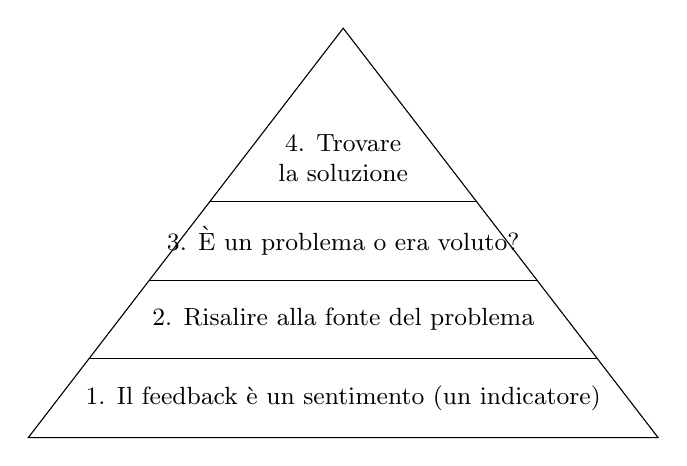
\begin{tikzpicture}[font=\small]
  \draw (0,0) -- (8,0) -- (4,5.2) -- cycle;
  \draw (0.77,1) -- (7.23,1);
  \draw (1.54,2) -- (6.46,2);
  \draw (2.31,3) -- (5.69,3);
  \node at (4,0.5) {1. Il feedback è un sentimento (un indicatore)};
  \node at (4,1.5) {2. Risalire alla fonte del problema};
  \node at (4,2.5) {3. È un problema o era voluto?};
  \node[align=center] at (4,3.55) {4. Trovare\\ la soluzione};
\end{tikzpicture}
\caption{La piramide del feedback come la descrive il relatore: si parte
dalla sensazione riferita da chi dà il feedback e si sale fino alla
soluzione. Ricostruzione schematica; la slide originale non è
disponibile.}
\label{p0:fig:piramide}
\end{figure}

\subsection{I feedback duri}

La piramide è anche un ottimo modo per \textbf{ricevere feedback in modo
professionale}, anche quelli difficili. Il relatore dà spesso feedback
\textbf{duri} ``anche per testarvi'': ``non perché sono stronzo''. Può dire
che una task è ``decente'', e dire anche tutto ciò che è sbagliato;
bisogna ricordarsi di lavorarci sopra e di \textbf{non prenderla sul
personale}. Magari sta testando la reazione, ``perché di fronte al vostro
capo in un'azienda non potete mandarlo a fanculo''.

% ---------------------------------------------------------------------
\section{La tecnica dell'iceberg}
\label{p0:sec:iceberg}

E se il problema è insormontabile? ``Allora, se il problema è
insormontabile, non esiste'', perché il relatore ha imparato la
\textbf{tecnica dell'iceberg} e la racconta ``come mi è stata spiegata''.
Non ha una base scientifica, avverte, ma a livello psicologico lo ha
aiutato molto. È una tecnica di \textbf{categorizzazione dei problemi}: non
è detto che un problema si risolva ``così'', ma la prima cosa da fare quando
lo si affronta è \textbf{descriverlo}, scriverlo in un testo, farne uno
schemino, e cercare di \textbf{classificarlo} in uno di quattro iceberg
(tabella~\ref{p0:tab:iceberg}). Se ne possono anche inventare di nuovi, per
esempio un iceberg ``basso e lungo'', che si estende per molto spazio invece
di essere largo.

\begin{table}[htbp]
\centering
\small
\begin{tabular}{@{}lp{4.4cm}p{5.4cm}@{}}
\toprule
\textbf{Iceberg} & \textbf{Che problema è} & \textbf{Come si affronta} \\
\midrule
\textbf{Alto} & Molto alto, insormontabile se lo si vuole scavalcare. &
Non lo si può prendere di petto: va \textbf{aggirato} in qualche modo. \\
\textbf{Largo} & Semplicemente molto grande, ma poco difficile. & Ci si
mette lì e \textbf{si fa fatica}. \\
\textbf{Nascosto} & Contiene situazioni problematiche, problemi nascosti. &
Obbliga a trovare il \textbf{problema reale} e a risolvere prima quello. \\
\textbf{Mostruoso} & Grande, difficile, complesso. & Richiede un
\textbf{approccio sistematico}, di solito suddividendolo in più parti. \\
\bottomrule
\end{tabular}
\caption{I quattro iceberg della tecnica dell'iceberg, come li presenta il
relatore.}
\label{p0:tab:iceberg}
\end{table}

Perché descrivere un problema con una forma ``geografica'' aiuta? Perché, se
lo si è descritto correttamente, si trova il modo di risolverlo. E, aggiunge
il relatore, la maggior parte delle volte si noterà che
\textbf{suddividere un problema in più parti} è la scelta migliore:
``splittate il problema in più parti, razionalizzate il problema''. Ed è
questo, conclude, il modo per affrontare al meglio il primo anno di AIV, o
tutti e tre.

% ---------------------------------------------------------------------
\section{Le domande finali}
\label{p0:sec:domande}

``Domande? Così recupero.'' E poi, davanti al silenzio: ``Oh, che
cavalcata! No, dai, vi prego, ditemi che avete dei dubbi''.

\subsection{A che cosa serve lo zone out?}

Una studentessa non ha capito il vantaggio dello zone out. Il relatore lo
spiega con la slide di figura~\ref{p0:fig:modi}: lo zone out
\textbf{potenzia la modalità diffusa}, e quindi la possibilità di trovare
soluzioni \emph{out of the box} che non si trovavano perché ci si
focalizzava troppo su un singolo punto. Se la soluzione è ``qui'' e ci si sta
concentrando ``qua'', non ci si arriva; in modalità diffusa il cervello vaga
e a un certo punto impatta nella soluzione. Inoltre rilassa la mente e, così
facendo, attiva il consolidamento, trasformando la working memory in
long-term memory. (Un partecipante commenta che sembra il cervello di un
personaggio di un film d'animazione\footnote{La trascrizione dice ``sembra
il cervello di Infeldo Sghetto 3'': il riferimento non è ricostruibile,
forse \emph{Inside Out}.}; ``vabbè, sì, certo, da qualche parte dovrà pure
venire fuori''.)

\subsection{La soluzione arriva sotto la doccia: e poi?}

Gabriele chiede: se finisco la giornata di lavoro con un problema aperto e
la soluzione mi viene a casa, sotto la doccia, mi rimetto a lavorare o me la
tengo per il giorno dopo? Nessuna delle due: \textbf{ci si prendono degli
appunti}. La tecnica migliore è avere sempre con sé un taccuino o il
cellulare (``non si dovrebbe fare, meglio un taccuino''). Il relatore tiene
il cellulare sul comodino: a volte, di notte, tornando dal bagno, gli viene
in mente qualcosa e se lo segna; a volte, fuori con il cane, si registra
mentre parla, e a volte si sblocca proprio parlando.

Tutto ciò che si è visto oggi, aggiunge, verrà ripreso durante il primo
anno, ma sono concetti che ``precedono il corso stesso'': durante l'anno non
c'è tempo, si fa il proprio corso. Qualcosa di neurocognitività tornerà a
narrative design e, al secondo anno, a game design, perché aiuta moltissimo
a \textbf{mappare il cervello del giocatore}, a capire come stimolarne certe
reazioni. Sarebbe bello approfondire, ma ``un po' rimane anche a voi'':
prendere le slide, approfondirle, leggerle.

\subsection{Arrivare da un'altra accademia}

Gabriele comincia direttamente dal secondo anno, avendo già fatto un anno in
un'altra accademia (``che purtroppo poi si sa com'è andata''); teme di
trovarsi spaesato non tanto per gli argomenti quanto per il metodo. Il
relatore distingue: \textbf{il metodo di studio è dello studente}; è il
\textbf{metodo di insegnamento} a essere diverso, e lo è (``senza nulla
togliere ai colleghi''): c'è un motivo per cui AIV fa nove ore di lezione a
settimana e il resto lo lascia allo studente. I consigli:
\begin{itemize}
  \item affrontare l'anno con \textbf{mentalità aperta}, senza crearsi
        pregiudizi solo perché arrivano cose diverse da quelle a cui si è
        abituati (e vale per tutti);
  \item se qualcosa non torna con l'istruzione precedente, \textbf{fare
        domande}, anche provocatorie: il relatore adora quando uno studente
        gli dice ``prof, questa cosa del viaggio dell'eroe io non la
        condivido, parliamone'' (``non vedo l'ora, davvero''), ``perché si
        apprende meglio''; avrebbe un problema se, da non professionista, si
        rifiutasse di rispondere per paura di come rispondere;
  \item ricordare che non è il metodo di insegnamento a cambiare lo
        studente: è il suo metodo di studio, ed è l'argomento ciò che si
        impara davvero, non il modo (``poi il modo aiuta molto, me ne rendo
        conto'').
\end{itemize}
Il problema vero, prevede il relatore, non sarà il metodo, ma il fatto che i
compagni hanno già un anno alle spalle e hanno affrontato cose che Gabriele
non ha visto, e su cui dovrà aggiornarsi. Il consiglio ``spassionato'':
\textbf{fare amicizia, aprirsi agli altri}. Ci si può far male, ``fa parte
del gioco''; ma essere aperti non vuol dire ``dare la propria password a
tutti'' (``a volte gli studenti mi prendono troppo alla lettera''): vuol
dire \textbf{dialogare}, e dialogare ``batte qualsiasi cosa''. Creare una
buona sinergia con la classe, cercando compromessi se serve.

\subsection{Come accorgersi di stare imparando un metodo sbagliato?}

Federico chiede come ci si accorge di stare imparando un metodo sbagliato,
per evitare il ``polso del chitarrista''. In parte sono i docenti a dirlo,
con i feedback: certe cose lo studente non può capirle da solo. Altre invece
le si nota confrontandosi con i compagni: ``cavolo, ma a me questa cosa
viene difficile, perché?''; ``mi viene, ma la sento macchinosa,
arzigogolata''. È possibile, non certo, che si stia avviando un effetto
Einstellung: si sta forse aprendo la bottiglia con una forza esercitatissima,
quando ne servirebbe molta meno.

\subsection{E all'università?}

Filippo, che frequenta anche l'università, chiede se questi metodi si
applichino a contesti più teorici, con meno possibilità di cambiare medium.
Il relatore premette di parlare ``con le pinze''. Ha fatto l'università e
``se ne pente parzialmente'': secondo lui l'università italiana ha
``tantissime competenze e conoscenze, ma pessime metodologie di
preparazione''; è soprattutto un istituto di ricerca e di studio, tranne le
facoltà pragmatiche (suo fratello è ingegnere elettrotecnico, con dottorato,
e doveva letteralmente fare circuiti; medicina è molto pratica). Ci sono
università di game design in Italia, ma con limiti: il ministero impone
esami come storia del videogioco, ``che è molto utile, ovviamente''.

Lui lavora per lo più con clienti, e al cliente non interessa la teoria né la
storia del videogioco fine a se stessa. La storia è utile \textbf{quando la si
applica}. Esempio, ripreso da ``stamattina'': il fatto che \emph{Pac-Man}
rallenti impercettibilmente mangiando i pallini\footnote{Si veda il
capitolo sul narrative design (sezione~\ref{p3:sec:mindset}). Il dettaglio
storico è che Pac-Man si ferma per un fotogramma a ogni pallino mangiato,
risultando un po' più lento dei fantasmi nei corridoi pieni di pallini.}
serve se un giorno, al lavoro, bisogna far rallentare il personaggio, senza
che il giocatore se ne accorga, quando fa certi passi, per renderlo più
raggiungibile e dargli la sensazione di ``oddio, non ce la faccio!'', magari
in una scena molto tesa di un horror: si prende la soluzione di Pac-Man e la
si adegua al contesto.

È molto importante che esista la ricerca: AIV ha bisogno degli studiosi,
il relatore lavora spesso con consulenti esperti di antropologia o di
storia. Ma non crede che un neolaureato sia pronto per l'industria, perché
molte tecniche della game industry non si insegnano all'università e
viceversa. Cita, senza nominarlo, uno studioso americano diventato un
professore importantissimo, che pubblica saggi di game design: saggi che
mostrano non un'incapacità di comprendere i framework, ma una comprensione
``in una scatola chiusa'', perché non li ha mai visti all'opera in un gioco.
È la differenza fra imparare a riparare un motore e fare davvero il
meccanico, quando le cose non sono uno a uno e vanno adattate.

Filippo precisa che la sua fatica all'università è data proprio dal ciclo
``testo, esame'', senza pratica, discussione e comunicazione. Il relatore
ribadisce che in AIV, in game design, tutte le task sono pratiche: al primo
anno su prodotti pubblicati (l'analisi del \emph{core loop} di un gioco, per
dire). All'università ci sono limiti: l'ultima volta che ha collaborato con
un ateneo gli hanno detto che il ministero impone un tetto del 30\% alle
attività di laboratorio. A lui il ciclo ``studio, studio, esame'' non
piace, perché nella vita reale non funziona così: ``il mio esame è la
pubblicazione'', che arriva dopo tre, quattro, cinque anni. Le conoscenze
generali che dà l'università sono ``imprescindibili ed enormi'', ma si
possono anche recuperare. Fa l'esempio della dizione nel doppiaggio: le
regole si assorbono, e al direttore interessa che la battuta sia detta bene;
e a volte, soprattutto gli americani, chiedono uno slang, e ``prova a
chiedere in università di farti imparare lo slang newyorkese di un
rapper''\footnote{La trascrizione dice ``addizione'' per ``dizione''. Il
passaggio è confuso, ma il senso è che certe competenze professionali si
apprendono sul campo, da altri professionisti, più che in università.}: gli
attori americani si formano facendo esperienza, andando da altri attori.

Non vuole criticare l'università: collabora con università e la rispetta. Ma
non gli piacciono quelli che, finito un corso universitario, pensano di
uscire e andare dritti a fare videogiochi. ``Io l'ho sentito sulla mia
pelle'': uscito dall'università non trovava lavoro e non capiva perché;
dieci anni dopo l'ha capito: quelle cose non le sapeva, e ha dovuto
``abbassare la cresta, fare un lavoro di umiltà e dire: ho studiato
altro''.

\subsection{Anatomia, per chi l'ha già studiata}

Una studentessa ha visto che al primo anno c'è anatomia e, avendo già fatto
tre esami di anatomia, chiede come sarà strutturato il corso. Va chiesto al
direttore di 3D art, nell'incontro dedicato (capitolo~\ref{p6:cap:3d}): il
relatore sa poco di quel corso, se non che al primo anno ci sarà una
collaborazione con i narrative per il \emph{world building} di un
gioco\footnote{Nella trascrizione: ``per il war building del giocato'',
probabilmente ``del giocattolo'': il corso di narrative prevede un modulo
di world building per i giocattoli (si veda il capitolo~\ref{p3:cap:narrative}).};
``vi diremo tutto a tempo debito'', in primavera.

\subsection{Le fiere: chi paga?}

Ultima domanda: se uno degli eventi di settore richiesti per il certificato
di eccellenza (sezione~\ref{p1:sec:eccellenza}) fosse una fiera come la
Gamescom, le spese sarebbero individuali? AIV fornisce \textbf{il biglietto
e l'alloggio} (dopo un'incertezza: ``vitto e alloggio\ldots\ scusatemi,
biglietto. No, alloggio'') ma non il trasporto, per \textbf{una fiera
all'anno}, a chi ha acquistato l'opzione \emph{Experience}; ``c'è scritto
sul sito''. La fiera la decide AIV ogni anno, sulla base di quella più
indicata; al terzo anno è al cento per cento la \textbf{First
Playable}\footnote{La trascrizione dice ``force playable''. La First
Playable è l'evento business dell'industria videoludica italiana che si
tiene a Firenze.}, ``perché alla First Playable bisogna andare''. A volte
le fiere mandano sconti, e la segreteria li comunica su Discord:
``sfruttateli assolutamente''. Ma AIV non ha la forza economica di mandare
tutti in fiera, solo chi ha l'Experience. Il relatore, che è di Milano, alla
Milan Games Week di solito scrive un messaggio per organizzare un
\emph{meet up}. La Gamescom è ``estremamente costosa'' anche da soli: chi
vuole andarci con AIV deve avere l'Experience, altrimenti si paga biglietto
e albergo. E la fiera, ogni anno, cambia.

%    % =====================================================================
%  Professioni 1 — I Dev Days: il metodo di AIV e i Dev Projects
%  Fonte: trascrizione dell'incontro di apertura dei Dev Days (AIV1):
%  un incontro online su Zoom di un'ora, il lunedì mattina della prima
%  settimana del primo anno, tenuto da Daniele Fusetto (direttore del
%  corso di narrative design e brand advisor dell'Accademia Italiana
%  Videogiochi) con Andrea Morini (direttore della didattica). Circa 31
%  partecipanti collegati su un centinaio di iscritti al primo anno;
%  slide condivise, un video di gioco senza audio, domande in chat.
%  Pacchetti richiesti nel preambolo del libro:
%    \usepackage[utf8]{inputenc}, \usepackage{booktabs},
%    \usepackage{tikz} con
%    \usetikzlibrary{arrows.meta,positioning,calc,fit}
%
%  Collocazione nel libro: parte "Alcune Professioni nel Mondo
%  Videoludico", dopo AIV0_mindset_e_best_practice (3.2).
%  Tutte le etichette di questo capitolo hanno il prefisso "p1:".
%  Il capitolo AIV0 (prefisso "p0:") rimanda a questo; questo rimanda ai
%  capitoli delle singole professioni (AIV2-AIV6).
%  La figura è una ricostruzione schematica di quanto il relatore spiega
%  con le slide, non una copia delle slide.
% =====================================================================

\chapter[I Dev Days e il metodo di AIV]{I Dev Days: il metodo di AIV,
la collaborazione fra discipline e i Dev Projects}
\label{p1:cap:devdays}

Ogni anno accademico, all'Accademia Italiana Videogiochi (\textbf{AIV}),
comincia con una settimana di incontri chiamati \textbf{Dev Days}. Lo scopo
è duplice: \textbf{impostare il lavoro} dell'inizio dell'anno e
\textbf{presentare a tutti gli studenti del primo anno che cosa faranno i
colleghi degli altri corsi}, perché, come si sentirà ripetere molte volte,
``la gaming industry è fortemente collaborativa'': i giochi si fanno in team,
e per lavorare bene con un game designer, un narrative designer, un
animatore, un programmatore o un 3D artist bisogna sapere che cosa fanno.
Questo capitolo raccoglie l'\textbf{incontro di apertura}; i capitoli
successivi raccolgono le presentazioni dei singoli corsi, cioè delle singole
professioni: game e level design (capitolo~\ref{p2:cap:gamedesign}),
narrative design (capitolo~\ref{p3:cap:narrative}), character animation
(capitolo~\ref{p4:cap:animation}), programmazione
(capitolo~\ref{p5:cap:programming}) e 3D art (capitolo~\ref{p6:cap:3d}).

A condurre l'incontro è \textbf{Daniele Fusetto}, direttore del corso di
narrative design e \emph{brand advisor} di AIV, che insegna in AIV dal 2019 e
in generale dal 2016; con lui c'è \textbf{Andrea Morini}, \textbf{direttore
della didattica}, che interviene a più riprese. L'incontro si tiene online,
su Zoom, il lunedì mattina, e dura \textbf{un'ora} (``abbiamo un'ora di tempo,
purtroppo''): non si aspetta molto chi è in ritardo, anche perché la
registrazione verrà caricata sulla piattaforma dell'accademia
(\emph{l'hub}). L'incontro non è facoltativo: ``i Dev Days non sono degli
incontri facoltativi'', bisogna almeno vederli in registrazione, ``altrimenti
si rischia di rimanere indietro fin dall'inizio''. Negli anni in cui
Fusetto e Morini hanno insegnato, ``sottovalutare una cosa del genere è di
solito il primo sintomo che qualcosa non va''.

Due avvertenze di lettura. La prima: la trascrizione è automatica e storpia
quasi sempre il nome dell'accademia (``Hive'', ``IVE'', ``Ive'', ``AIB'',
``AB'', ``IV'') e diversi titoli e termini; il capitolo usa sempre
``AIV'' e segnala in nota le ricostruzioni incerte. La seconda: molte
affermazioni riguardano l'organizzazione di AIV (calendari, regole,
certificati, opzioni di iscrizione) e valgono per l'anno a cui l'incontro si
riferisce; sono riportate come le dicono i relatori.

La data, dedotta, è \textbf{lunedì 5 ottobre 2026}\footnote{La data non è
detta. Si ricava da tre indizi: le lezioni dei corsi cominciano
``ufficialmente'' il 19 ottobre, quelle di narrative ``questo venerdì''; nel
capitolo sul narrative design, il giorno dopo, il relatore fissa la prima
lezione di narrative a ``venerdì 9 ottobre''; e nel 2026 il 9 ottobre è
venerdì. È una deduzione.}.

Il percorso del capitolo:
\begin{enumerate}
  \item l'avvio e la politica della webcam (sezione~\ref{p1:sec:avvio});
  \item che cosa sono i Dev Days e il calendario della settimana
        (sezione~\ref{p1:sec:devdays});
  \item il \textbf{metodo di AIV}: che cosa non si tollera e quattro cose da
        fare (sezione~\ref{p1:sec:metodo});
  \item \textbf{best practice} e \textbf{trappole}
        (sezioni~\ref{p1:sec:best} e~\ref{p1:sec:trappole});
  \item gli \textbf{obiettivi} dei corsi: portfolio, lavoro di gruppo,
        competenze trasversali (sezione~\ref{p1:sec:obiettivi});
  \item l'attestato di partecipazione e il \textbf{certificato di
        eccellenza} (sezione~\ref{p1:sec:eccellenza});
  \item i \textbf{Dev Projects} del secondo anno e la pipeline di sviluppo,
        con il caso di \emph{Beat of Rebellion}
        (sezioni~\ref{p1:sec:devprojects}--\ref{p1:sec:beat});
  \item perché parlarne il primo giorno, i falsi miti e le domande finali
        (sezioni~\ref{p1:sec:perche}--\ref{p1:sec:domande}).
\end{enumerate}

% ---------------------------------------------------------------------
\section{L'avvio}
\label{p1:sec:avvio}

Si comincia con qualche minuto di attesa: alcune persone sono in ritardo
``per problemi di hub'' o perché non hanno ancora fatto l'accesso. Il
relatore disabilita la sala d'attesa di Zoom e raccomanda di tenere
d'occhio il \textbf{Discord di AIV} e la propria \textbf{mail}. Poi
condivide le slide e comincia con la parte ``molto introduttiva'', mentre
arrivano gli ultimi.

\subsection{La webcam}

``Possibilmente accendete la webcam'': il relatore vuole vedere facce sveglie
``e anche le vostre camerette''. ``Mamma mia, è lunedì mattina per tutti'':
non c'è una regola che imponga di presentarsi a lezione ``belli e col volto
riposato'', ma la regola è che \textbf{ci si fa vedere}, anche quando si
segue da remoto. Non solo per buona educazione: i docenti devono vedere le
facce, le reazioni, e vogliono conoscere gli studenti anche fisicamente. Già
al tempo del COVID, ricorda, riconoscere dal vivo le persone viste online o
con la mascherina era stato ``un dramma''.

% ---------------------------------------------------------------------
\section{Che cosa sono i Dev Days}
\label{p1:sec:devdays}

L'agenda della mattina: che cosa sono i Dev Days, qual è il \textbf{metodo di
AIV}, e i \textbf{Dev Projects}, ``una cosa che voi vedrete al secondo
anno'', ma di cui i relatori vogliono dare un assaggio fin da oggi ``per
farvi capire che qua non si scherza''\footnote{La trascrizione dice
``farvi la capatanza'' e poi ``capatanta'': il senso è ``farvi fare una
capatina'', dare un assaggio. Il nome dei progetti del secondo anno
oscilla nella trascrizione fra ``Game Dev'', ``Dev Project'' e ``The
Projects''; il capitolo usa ``Dev Projects'' per i progetti e ``Game Dev''
per il percorso del secondo anno in cui si svolgono.}.

\subsection{Un'industria che lavora in team}

I Dev Days sono incontri dedicati, all'inizio del primo anno, a presentare
ciò che faranno gli altri colleghi e a impostare il lavoro. Il motivo è che
l'industria è fortemente collaborativa: \textbf{si sviluppano giochi in
team}, ``dalle 20 persone alle 400 persone''. Ci sono anche team più
piccoli, ma spesso un team di tre, quattro, cinque persone lavora molto con
\textbf{freelancer}. Esempio: si dice che \emph{Clair Obscur: Expedition 33}
sia stato fatto da trenta persone; ``non è vero, se vedete i credit, sono
400''\footnote{La cifra di 400 è del relatore. Il nucleo dello studio
Sandfall Interactive era di circa trenta persone; i titoli di coda includono
però numerosi collaboratori esterni (musica, doppiaggio, animazione,
outsourcing, localizzazione), che è appunto il punto del relatore.}. Fare
un gioco richiede un lavoro di team.

Al primo anno ognuno fa la propria disciplina: chi fa programmazione fa
programmazione, chi fa 3D fa 3D, e così per game design, character
animation, narrative design. Poi, all'inizio del secondo anno, ci si
incontrerà con tutti gli altri ``per fare insieme un videogioco''. Ma fin da
oggi bisogna capire che cosa faranno i colleghi e quali sono le altre
professioni insegnate in AIV, ``per meglio collaborare con gli altri''.

\subsection{Il calendario della settimana}

Per questo la settimana prevede \textbf{cinque incontri}, uno per ciascun
corso di AIV. Vanno seguiti \textbf{tutti}, e non sono solo per gli studenti
del corso presentato: ``sono per tutti gli studenti''. La presentazione di
game design spiega che cosa faranno i game designer durante l'anno, e la
devono seguire tutti, così che l'anno dopo, collaborando con loro, si sappia
più o meno che cosa fanno di solito. Lo stesso per narrative design,
character animation, programmazione e 3D art. L'obiettivo non è spiegare agli
studenti di quel corso che cos'è il corso (lo vedranno durante l'anno), ma
spiegare \textbf{a tutti} che cosa fanno le altre discipline. Tanto che
``probabilmente è meglio se, per esempio, la presentazione del corso di
programming la seguono più attentamente quelli che non faranno
programming''.

In più:
\begin{itemize}
  \item un incontro aggiunto quest'anno, il \textbf{giovedì mattina}, di
        un'ora e mezza, con Fusetto, anch'esso obbligatorio, sulla
        \textbf{comprensione del testo} (capitolo~\ref{pt:cap:comprensione}): ``mi spiace dirlo, ma negli ultimi
        anni ci siamo accorti che è difficile arrivare all'inizio di AIV con
        delle capacità di comprensione del testo ottime''. Non si parla di
        italiano di base né di una disciplina, ma di \textbf{comprendere
        ciò che le persone dicono e vogliono}, rispondere correttamente alle
        richieste dei docenti, evitare incomprensioni; si vedranno anche
        trucchi per comprendere meglio e per segnarsi le cose in modo da
        \textbf{saper porre domande}, ``perché è importantissimo porre
        domande'';
  \item un incontro il \textbf{martedì pomeriggio alle 14:30}, solo per chi
        si è iscritto entro il 31 luglio con la \textbf{Gamer Promo} o la
        \textbf{Dev Promo}: un incontro di \emph{mindset} e \emph{best
        practice} sulle pratiche migliori per imparare e apprendere
        durante l'anno (è il capitolo~\ref{p0:cap:mindset});
  \item per gli stessi studenti, la possibilità di una
        \textbf{mentorship} di un'ora con un tutor o un docente, ``per
        partire al meglio''. ``Sfruttatele, queste ore, perché l'anno scorso
        nessuno l'ha usata e poi dopo saltano fuori i problemi.'' Chi non
        ricorda se ha la promo può chiedere in segreteria.
\end{itemize}

% ---------------------------------------------------------------------
\section{Il metodo di AIV}
\label{p1:sec:metodo}

\subsection{In AIV si boccia}

``In AIV si boccia.'' Non è un'accademia ``dove vieni, paghi e passi
l'anno'': ci sono dei criteri. Il criterio principale è \textbf{non
consegnare le attività}, le cosiddette \textbf{task}, richieste durante
l'anno, perché la valutazione si fa su quelle: se non vengono consegnate, i
docenti non possono valutare.

Ma contano anche le \textbf{soft skill}, ``e se avete frequentato il nostro
open day lo sapete'': per passare l'anno bisogna
\begin{itemize}
  \item \textbf{interagire}: non isolarsi; chi è un po' introverso cerchi di
        uscire, di chiedere, di porre domande;
  \item \textbf{rispettare gli altri};
  \item essere \textbf{proattivi}: se viene in mente oggi che si deve o si
        può fare una cosa, non la si rimanda a domani; se si ha una domanda
        per la prossima lezione e si sa che il docente è raggiungibile per
        mail o per messaggio, non si aspetta la lezione.
\end{itemize}

\subsection{Tolleranza zero: bullismo, pregiudizi, cheating}

Su tre cose non c'è tolleranza.
\begin{description}
  \item[Bullismo.] ``Self-explanatory'', in tutte le sue forme: qualunque
        prevaricazione, anche implicita, ``non esiste''. Massima
        collaborazione e massima gentilezza, sempre.
  \item[Pregiudizi.] Si è in tanti e molto diversi, ognuno con le sue
        opinioni; ``a meno che voi non abbiate problematiche di tipo,
        diciamo, criminale, ma non credo'', bisogna partire dal presupposto
        che la persona che si ha davanti ha una sua storia, mettersi nei
        panni degli altri e \textbf{sospendere il giudizio}.
  \item[Cheating.] Fino a qualche anno fa voleva dire copiare dai compagni,
        avvantaggiarsi, manipolare la classe o i compagni per ottenere
        vantaggi non legati alla performance (``non faccio bene le attività,
        ma sono bravo a manipolare l'ambiente in modo da passare''). Negli
        ultimi due anni si è aggiunto \textbf{l'uso dell'IA}: è cheating
        quando, in un corso, viene detto di non usarla in un certo modo e la
        si usa così. Ogni corso ha il suo approccio (programmazione diverso
        da narrative, da game design, da character animation) e verrà detto
        che cosa si può fare e che cosa no. In narrative design, per
        esempio, è \textbf{severamente vietato scrivere con l'IA} per tutti
        e tre gli anni, ``vietatissimo'', fino a una lezione in cui il
        relatore spiegherà ``qual è l'unico modo, a mio parere'' per farsi
        aiutare dall'IA nell'atto della scrittura.
\end{description}

Ma cheating è anche copiare dai compagni: ``è successo, ce ne accorgiamo''.
I docenti vedono i compiti, notano forme usate nelle attività o
``spennellature, scolpiture nel modello 3D'' troppo simili. ``D'altronde, se
molti critici hanno capito che Palworld aveva copiato da Pokémon anche i
modelli 3D, si può fare''\footnote{È l'opinione del relatore, riportata
com'è. Le somiglianze fra i modelli di \emph{Palworld} e quelli dei Pokémon
sono state sostenute da utenti e commentatori dopo l'uscita del gioco
(2024), ma non sono mai state accertate; la causa intentata da Nintendo e
The Pokémon Company contro lo sviluppatore riguarda la violazione di
brevetti, non la copia dei modelli.}. Nel cheating c'è sempre una vittima,
la persona sfruttata o manipolata; ma soprattutto chi bara \textbf{fa un
danno a se stesso}: ``state pagando per imparare. Imparare voi.'' Chi usa
scorciatoie per passare l'anno e poi si ritrova senza conoscenze ha perso
un'occasione.

\subsection{Inquiry-based learning}

Poi ``quattro cose che dovete fare''. La prima: tutti i corsi di AIV sono
\textbf{inquiry-based}. ``Non esistono domande stupide, soprattutto il primo
anno.'' Molti studenti scrivono ``ho una domanda stupida'': no, non ce ne
sono. Arriva proprio in quel momento una domanda in chat (``scusi, ma i
corsi che ha fatto vedere prima sono online?''), e il relatore la usa come
esempio: ``anche qua, ragazzi, è importantissimo, \textbf{specificate bene
nelle domande}''. Si intende la \emph{lezione}, cioè il singolo incontro, o
il \emph{corso}, cioè tutto il corso? Gli incontri di questa settimana sono
tutti da remoto. Sara ha fatto una domanda ``per niente stupida'', perché
non era chiaro, ``e ha imparato anche qualcosa''\footnote{Nel capitolo sul
narrative design (sezione~\ref{p3:sec:skill}) il relatore torna su questo
episodio per spiegare perché tiene tanto alla precisione dei termini.}.
``Meno domande fate, meno imparate.''

\subsection{Un ambiente simulativo del mondo del lavoro}

La seconda: AIV è un \textbf{ambiente simulativo del mondo del lavoro}.
Tranne game programming, che ha test ed ``esamini'' (e i docenti di quel corso
spiegheranno perché), \textbf{non ci sono sessioni d'esame}, ma valutazioni
verbali tramite \textbf{task}. Durante molte lezioni, non tutte, il docente
dirà: ``voglio che mi consegniate questa task entro questa data''. Se la si
manca, la task è mancata e conta per il non passaggio dell'anno. Le task non
hanno tutte la stessa durata: in alcuni corsi sono molto corpose e
richiedono mesi; in game design e narrative sono più equilibrate, con task
da una o due settimane e altre da mesi. In sintesi: task settimanali,
mensili, trimestrali o annuali.

Bisogna entrare a poco a poco nell'ottica di un \textbf{approccio
professionale} al corso: ``prendetelo un po' come un lavoro''. Ogni giorno
si deve produrre, studiare, apprendere, confrontarsi, fare call, come in
qualsiasi lavoro, non solo nei videogiochi. La puntualità è importante;
tutti gli aspetti professionali ``in senso lato'' non sono semplicemente
graditi, ``sono mandatori''. ``Molto di più di quando i genitori ci dicevano,
alle superiori, devi pensare alla scuola come a un lavoro: questo è molto più
veritiero.'' E come nel lavoro si fanno meeting e incontri, ma si lavora
anche molto da soli: non bisogna sottovalutare il peso delle attività.

Le task sono \textbf{opportunità} per migliorarsi, ottenere più feedback e
\textbf{farsi notare dai docenti}, perché il 99\% dei docenti di AIV sono
lavoratori del settore: Fusetto stesso lavora nell'industria, sta facendo dei
giochi in questo periodo, e alcuni suoi studenti lavorano con lui. ``Non è un
modo per essere assunti'', ma permette di farsi notare per le proprie
capacità.

\subsection{Fail to learn}

La terza: \textbf{fallire}. Una delle cose più importanti da fare al primo
anno è fallire e imparare: non \emph{fail for}, ma \emph{fail to
learn}\footnote{Così nella trascrizione; il senso è ``fallire per
imparare''.}. Se si sbaglia, si ricevono feedback e si trovano soluzioni, e
piano piano si impara a trovare soluzioni ai propri fallimenti; si noterà
``un aumento notevole'' delle proprie capacità. Il consiglio pratico:
prendere una task di settembre, metterla ``in una giara virtuale'' (un
drive), lasciarla lì e a gennaio confrontarla con una task di gennaio. Se le
differenze non si notano, è perché non si è fallito e non si è imparato: ``è
una campanella d'allarme''.

\subsection{Mettere in pratica, ogni giorno}

La quarta: i corsi di AIV richiedono di \textbf{mettere in pratica} ciò che
si apprende. Perché solo \textbf{nove ore di lezione a settimana}, e non
lezioni tutte le mattine come in altre accademie? Perché bisogna avere il
tempo di mettere in pratica teoria e pratica viste a lezione: ``se io non vi
do almeno 20 ore alla settimana per mettere in pratica quello che vi insegno,
è difficile''. Il relatore porta il proprio esempio\footnote{Poco prima il relatore dice ``come diceva Andrea'': nella trascrizione i cambi di voce fra i due relatori non sono segnati, e l'attribuzione di alcuni passaggi è incerta. Qui, dal contesto (``io so programmare un pochettino'', ripetuto anche nel capitolo~\ref{p3:cap:narrative}), parla con ogni probabilità Fusetto.}: pur considerandosi un artista usa spesso Unreal Engine, e nel lavoro si acquisiscono capacità trasversali; sa
programmare ``un pochettino'', ma non ci riuscirebbe se non si mettesse
tutti i giorni quindici minuti a programmare\footnote{La trascrizione dice
``io non saprei programmare se io tutti i giorni mi mettessi lì 15 minuti a
programmare'': manca evidentemente un ``non''.}. Bisogna impegnarsi ogni
giorno nella propria disciplina. Altrimenti ci si sveglia all'ultimo, si
imparano le cose al momento del bisogno (magari anche bene), ma nasce una
sensazione di \emph{burnout}, ``e poi il burnout lo prendete''.

Quindi: mettersi da parte del tempo ogni settimana per applicare ciò che si
vede a lezione, farsi domande, fare domande ai docenti, e
\textbf{impegnarsi al massimo sulle task}. Con alcune regole:
\begin{itemize}
  \item se una task sembra \textbf{semplice}, la si fa \textbf{due volte}:
        forse si sta sopravvalutando se stessi. Se è davvero semplice, si
        chiede al docente se c'è la possibilità di avere qualcosa in più
        (``a me sembrava semplice, secondo te l'ho fatta bene?''), e magari
        arriva qualcosa di extra;
  \item se sembra \textbf{troppo difficile}, la si tenta comunque, perché
        una delle basi dell'apprendimento è l'\textbf{alternanza di
        difficoltà}: alternare task semplici e difficili fa apprendere
        meglio che fare solo le une o solo le altre;
  \item se la si finisce \textbf{in anticipo}, la si approfondisce e la si
        rifà. ``È noioso? Sì. È lungo? Sì. È pesante? Sì. Però è il
        migliore.''
\end{itemize}

\subsection{Consegnare in anticipo per avere un feedback?}

Una domanda in chat: si può consegnare una task in anticipo per ricevere un
feedback e correggere gli errori? Sì, risponde il relatore, ma con due
precisazioni. Di solito i docenti danno tutti i feedback contemporaneamente,
``perché ho bisogno di vedere anche il confronto con la classe''; si può
però mandare una task e fare \textbf{domande specifiche}. E bisogna
aspettarsi che i docenti non rispondano direttamente: a lui capita spesso
che gli chiedano ``Daniele, secondo te questa cosa l'ho spiegata troppo?
l'ho fatta troppo così?'', e lui risponde ``secondo te l'hai fatta
troppo?''. ``Non frustratevi per questo'': deve insegnare in qualche modo ad
andare avanti da soli. Non è detto quindi che si ottenga una risposta, ma si
avranno indicazioni, e chi consegna uno o due giorni prima può ricevere
feedback aggiuntivi. Una condizione: se si consegna in anticipo, deve
essere perché si è dato il massimo, non perché si è ``tirato via'' per
consegnare prima. E non è banale: nella sua carriera, ``ma anche
attualmente'', quasi nessuno riesce a consegnare in anticipo.

% ---------------------------------------------------------------------
\section{Best practice}
\label{p1:sec:best}

Le \textbf{best practice}, ``soprattutto per chi segue in remoto''.

\paragraph{Camera sempre accesa.} Vale per chi segue da remoto, ma anche per
chi segue in presenza e capita di seguire una lezione online. E capiterà:
``in Italia abbiamo una maledizione, si chiamano scioperi''. Spesso il
venerdì ci sono scioperi di mezzi, treni, autostrade, a Roma e a Milano
(``l'anno scorso Milano è stato un delirio''); per non perdere la lezione,
se c'è sciopero e il docente non può venire in presenza, la lezione del
venerdì si trasforma in lezione da remoto. In quei casi la camera va tenuta
accesa: al docente serve per vedere i volti (``vedo il volto di Mattia, di
Gabriele, di Emanuele, di Davide, vedo come sono messi, se stanno capendo
oppure no''), e allo studente è ``una scusa in meno per distrarvi'', perché
``la distrazione è sempre dietro l'angolo''.

\paragraph{Prendere appunti.} Cartacei o digitali, non importa. Non bisogna
fare come i camerieri, che pensano di prendere gli ordini a mente e
puntualmente se li dimenticano; il fenomeno ha anche un nome, l'\textbf{effetto
Zeigarnik}, ``se volete potete andarlo a cercare''\footnote{La trascrizione
dice ``Zygarnik Effect''. L'effetto è ripreso e discusso nel
capitolo~\ref{p0:cap:mindset} (sezione~\ref{p0:sec:memoria}).}.

\paragraph{Interagire con i docenti.} Fare domande durante le lezioni.

\paragraph{Rivedere le registrazioni.} Soprattutto per gli
\textbf{studenti lavoratori}. Ogni settimana ci sono nove ore di lezione; chi
lavora e sa che ne perderà tre a settimana ha il compito ``tassativo'' di
recuperarle nel weekend. Altrimenti la settimana dopo diventano sei, poi
nove, ``e improvvisamente quelle tre ore diventano 18''. ``Io ho studenti che
arrivano a giugno e mi dicono: prof, devo ancora recuperare lezioni di
febbraio. E io non rido'', perché le lezioni sono spesso consequenziali. Il
sistema di registrazione dà pochi problemi: entro 24 ore circa le
registrazioni sono disponibili (``scongiurando bug e problematiche di
cloud''). ``Guardatevele, riguardatevele, mettete il 2x piuttosto.''

\subsection{Quanto restano le registrazioni, e a che cosa servono}

A una domanda in chat uno dei relatori risponde che le registrazioni restano
attive almeno fino all'inizio dell'anno successivo, verso fine settembre,
quando si cominciano a staccare le vecchie per fare spazio al nuovo anno.
Si possono quindi recuperare anche d'estate: chi, per motivi di lavoro, non
ha consegnato abbastanza e ha bisogno di tempo per recuperare, lo ottiene
durante l'estate, con l'accesso alle lezioni.

Le registrazioni, aggiunge Fusetto (richiamando un'osservazione di Morini), servono anche ad altro: ci
saranno cose che non riescono, problemi che non si risolvono, cose non
capite. È vero che i docenti sono facilmente raggiungibili su Discord, ma
quella è \textbf{l'ultima chance}: bisogna imparare a \textbf{risolvere i
problemi da soli}. Se è qualcosa trattato a lezione, si riguarda la
registrazione, si chiede ai colleghi, si guardano gli appunti e le
dispense; si chiede a Google (``non riesco a installare questa cosa''), si
chiede ``alla maledettissima intelligenza artificiale''. Solo se nulla di
tutto questo aiuta, perché il problema è particolarissimo, si va dal
docente. Bisogna sforzarsi di non avere ``la pappa pronta'': fa parte del
\emph{problem solving}. È come con un datore di lavoro: non si va dal capo a
ogni problema, prima si cerca di risolverlo. Al primo anno, precisa
Fusetto, va bene scrivere qualsiasi domanda quando si vuole (e così per gli
altri docenti, secondo le indicazioni che daranno); al secondo anno
comincerà a dire ``guarda che per questa cosa potevi anche non scrivermi'',
perché nel lavoro non si può scrivere al capo ``ogni due per tre''.

Chi ha bisogno di ancora più tempo ha l'opzione \textbf{Companion},
acquistabile anche durante l'anno accademico, che dà accesso alle lezioni
per un altro anno: è pensata per chi ha davvero bisogno di più tempo, e
richiede un processo dedicato (le lezioni vengono spostate su un altro
server), con più tempo, costo e lavoro. ``Non è un obbligo, ovviamente.''

% ---------------------------------------------------------------------
\section{Trappole}
\label{p1:sec:trappole}

Poi le \textbf{trappole}, ``trappoloni''.

\paragraph{``Mi basterà ascoltare?''} Molto spesso no.

\paragraph{``Posso fare altro nel mentre?''} ``Altro trappolone enorme, che
l'anno scorso ha fatto cadere tantissime persone'': ``tanto sono indicazioni
di massima, poi mi rivedo la lezione''. No. Andrea Morini, ``come direttore
didattico, terribile'', avverte che i docenti sanno se, durante una lezione
da remoto, qualcuno guarda una serie TV o gioca; e ci sono stati studenti
che giocavano in aula mentre il docente spiegava. ``Non è ammissibile in
nessun caso, mai'': a quel punto interviene lui, ``io sono quello cattivo''.
Massima attenzione: \textbf{nessuno è multitasking}, ``è falso''. Si segue la
lezione e basta, si spegne il cellulare. Anche perché seguire più cose
contemporaneamente \textbf{affatica}, anche se non sembra.

\paragraph{``Farò due minuti di ritardo, che sarà mai?''} C'è un ritardo
ammesso di 5--10 minuti, ma \textbf{non c'è il quarto d'ora accademico},
a meno che il docente non lo conceda. Se il docente dice ``10:10 in aula'' o
``14:10 in aula'', a seconda dell'orario, o ``questo orario, \emph{sharp}'',
bisogna essere puntuali.

\paragraph{``Sono come tutorial.''} ``Questo è un grande altro tema'': il
trappolone del ``tanto è come un tutorial di YouTube, poi me lo seguo in
registrazione''. No: rispetto a un corso su YouTube, su Udemy o a un corso di
formazione registrato, si ha un vantaggio, \textbf{si può chiedere
direttamente al docente}, che è un esperto del settore (``nel corso di Udemy,
vi posso assicurare, non sapete chi è il docente''). Anche quando una
lezione è un tutorial, ``non è davvero un tutorial'': si può chiedere di
rispiegare. E, ricordando le soft skill (niente pregiudizi, rispetto), se un
collega chiede ``prof, può rispiegare?'' e noi avevamo capito, anche se
pensiamo di annoiarci, conviene pensare ``magari mi sono perso comunque
qualcosa''. ``Non è un errore rispiegare, anzi, molto meglio rispiegare.''

% ---------------------------------------------------------------------
\section{Gli obiettivi dei corsi}
\label{p1:sec:obiettivi}

\subsection{Obiettivi primari: portfolio, problemi reali, lavoro di gruppo}

Il primo obiettivo, tutto l'anno e tutti gli anni, è \textbf{lavorare per
realizzare un portfolio}. Oltre al ``pezzo di carta'', la cosa principale per
entrare nella game industry è il portfolio: i giochi creati, i prodotti
fatti, i modelli 3D per i 3D artist, il software per i programmatori, gli
script per i narrative designer, le task per i game designer, le animazioni
per i character animator.

Attenzione, ``soprattutto programmatori e 3D artist, che di solito
sottovalutano questo punto'': \textbf{i giochi pubblicati sono l'elemento di
portfolio più importante di tutti}, più degli altri giochi fatti e ancora di
più delle task. Quando un selezionatore delle risorse umane, ``ma soprattutto
un lavoratore di un'azienda videoludica'', valuta un portfolio, considera più
importanti i giochi pubblicati su itch.io o su Steam, anche con gli amici
per una jam (non devono essere tripla A, devono essere accessibili), di
qualsiasi elemento legato a giochi mai pubblicati. ``Ho fatto un modello 3D.
È stato pubblicato in un gioco? No? Vale di meno'', e vale ancora meno della
task. Per questo, andando avanti negli anni, bisognerà riuscire sempre di più
a realizzare giochi, e giochi pubblicati; e qui AIV aiuta con i Dev Projects.

Il secondo obiettivo è lavorare su \textbf{problemi e progetti reali}: c'è
``un implicito accordo'' fra docenti e studenti per cui i docenti danno
problemi che davvero si troveranno nell'industria, quelli che si affrontano
tutti i giorni. E il terzo è lavorare \textbf{in gruppo} per potenziare le
soft skill. ``Fondamentale'': bisogna creare fin dai primi mesi un
\textbf{ottimo corpo classe}, una buona sinergia fra studenti. Secondo i
numeri e le analisi di AIV (``e Andrea ve lo può confermare''), le classi
molto unite, con studenti che si supportano, hanno molte più possibilità e
meno problemi di quelle che litigano. ``È banale da dire'', eppure non si sa
quante volte micro faide e micro litigi nati per niente creino problemi
``atroci, enormi''.

Andrea Morini aggiunge che queste cose derivano spesso da una sbagliata
considerazione del proprio \textbf{ego}: ``qui non c'è ego''. Non vuole
vedere nessuno che, per motivi di ego, rallenti o danneggi i colleghi,
anche involontariamente, senza accorgersene e senza malizia, ``ma succede''.
``Qui l'ego lo potete mettere da parte, e allora andiamo tutti d'accordo.''

\subsection{Obiettivi secondari: competenze a T rovesciata}

Fra gli obiettivi secondari ci sono le \textbf{competenze a T
rovesciata}\footnote{La trascrizione dice ``competenze ti è rovesciata'' e
``competenza tirovesciata''. Il riferimento è al modello delle competenze
``a T'' (\emph{T-shaped skills}): una competenza profonda in una
disciplina (l'asta verticale) unita a una conoscenza più ampia delle
discipline vicine (il tratto orizzontale). Il relatore lo chiama ``a T
rovesciata'', con il tratto orizzontale alla base.}. Nell'industria si torna
a parlare del fatto che stanno tornando lentamente i \textbf{generalisti}.
È un ciclo costante dagli anni Settanta, da quando sono nati l'informatica e
il software: le industrie tecnologiche preferiscono, alternativamente,
persone con competenze variegate che sanno lavorare su tutto un prodotto (i
cosiddetti \emph{full stack}: programmatore full stack, game designer full
stack) oppure persone molto specializzate, \textbf{verticali}. Fino a prima
dell'IA era molto importante essere ``terribilmente verticali''; proprio in
questi giorni Fusetto e Morini si sono confrontati sul fatto che molte
aziende cominciano a pensare di tornare indietro e avere generalisti,
perché con l'IA c'è ``questa sorta di verità e illusione'' (``lo sapremo
solo con calma nel tempo'') che una persona con competenze differenti
funzioni di più.

AIV insegna a T rovesciata, e questo mette gli studenti in una sorta di
``bunker protettivo'': i corsi sono verticali, ma dentro la propria
verticalità si vedono tante cose. In game design si è verticali sul game
design, ma si vede Unreal, si programma con i Blueprint, si fa level design,
combat design: ``vedete tutto quello che c'è nel game design''. E nessuno,
nell'industria, chiederà a un game designer di fare modelli 3D: magari
competenze di base per mettere gli asset nell'engine, ``ma non vi potrete
sostituire a un modellatore 3D''. Bisogna quindi essere
\textbf{intraprendenti}: imparare tutte le sfaccettature del proprio lavoro
e, al secondo e terzo anno, nei lavori di team, imparare anche \textbf{per
osmosi} da ciò che fanno i colleghi.

Andrea Morini aggiunge un dettaglio: AIV ``si mette sempre in discussione''.
Un paio di volte l'anno va a vedere ``non so quante'' \emph{job
description}, le posizioni aperte, per verificare quanto sia vero che il
generalista sta tornando di moda: ``poco, poco''. Oggi le posizioni aperte
sono ancora ``estremamente verticali, non se ne esce''; nei piccolissimi
studi di tre o quattro persone un generalista può essere più apprezzato,
altrimenti no. Quindi, all'uscita, ci si propone come \textbf{specialisti
della propria disciplina}, e in azienda scopriranno che si sa fare anche
altro. Spesso si entra con una qualifica e si esce con un'altra (magari si
entra in un ruolo junior di base, ``adesso poi dovremo vedere che cosa
succederà con le posizioni junior''), e nulla vieta di fare carriera
all'interno.

\subsection{Competenze spendibili fuori dal settore}

Le competenze sono importanti anche per l'\textbf{extrasettore}: in tutti i
corsi si imparano cose spendibili anche fuori dalla game industry, e questo
serve per due motivi. Se non si trova lavoro nell'industria, si possono usare
altrove; e se dopo tre anni ci si convince che quello non è il proprio
futuro, idem. Fusetto ha ``moltissimi studenti'' che hanno cambiato carriera
usando le competenze acquisite. Si augura che tutti facciano il lavoro per cui
si sono iscritti, ma ``non abbiamo la palla di cristallo'': meglio prevenire
che curare.

Al terzo anno, inoltre, si fanno molte lezioni, anche con i \textbf{Career
Days}, sulle \textbf{competenze imprenditoriali} e sul
\textbf{freelancing}: non c'è solo l'assunzione in azienda, c'è il freelance
(Fusetto è freelancer) e c'è chi vuole aprire un'azienda. L'Italia, dice,
ha due cose ``fenomenali'': la capacità degli italiani di essere imprenditori
e di sognare in grande, e ``la stragrande capacità del governo italiano di
mettere burocrazia per impedire l'imprenditorialità''. Sulla burocrazia non
si può lavorare, ma si può diventare intraprendenti, evitare errori enormi e
diventare imprenditori migliori, ``per esempio degli americani'': un
americano apre una società in due ore con una carta di credito e al primo
problema si blocca; un italiano dice ``che sarà mai, ho passato ore
chilometriche a fare burocrazia''.

% ---------------------------------------------------------------------
\section{Attestato di partecipazione e certificato di eccellenza}
\label{p1:sec:eccellenza}

La parte sui certificati la presenta Andrea Morini. Da qualche tempo AIV ha
introdotto l'\textbf{attestato di partecipazione}, che attesta che si è
partecipato al corso, cioè che si è fatto ciò che il corso richiede:
\textbf{consegnare le task}. Non basta essere stati presenti (``è implicito
che è importante''); è ancora più importante \textbf{produrre}, così da potersi
confrontare su ciò che si produce.

Accanto c'è il \textbf{certificato di eccellenza}\footnote{La trascrizione
dice ``il CTV Audi Eccellenza'' e ``il certificato di scelta'': si tratta in
entrambi i casi del certificato di eccellenza.}, per chi dà importanza a
tutto ciò che si sta dicendo e applica queste best practice. I requisiti
sono tre:
\begin{enumerate}
  \item \textbf{aver prodotto molto e bene}: essere promossi, aver
        consegnato \textbf{tutte} le task dell'anno (``per alcuni corsi sono
        tante'') e superato gli eventuali test; oppure aver consegnato
        \textbf{almeno l'80\%} delle task, ma con \textbf{metà di questo 80\%
        valutata eccellente}, a discrezione del docente;
  \item \textbf{aver partecipato ai Dev Projects}, collaborando fino al
        \textbf{completamento} del progetto (non necessariamente alla
        pubblicazione); se per qualsiasi motivo non è stato possibile
        (``non perché lavorate, non potete'', ma perché il progetto è stato
        chiuso perché non andava bene, ``mille motivi''), aver partecipato
        almeno a delle \textbf{game jam}: ``è il \emph{second best}'';
  \item aver partecipato \textbf{almeno a un secondo evento di settore}
        ogni anno, oltre alla jam: ``sembra che dobbiamo metterla come un
        premio, e invece dovrebbe essere la prassi''.
\end{enumerate}

Gli eventi di settore sono fondamentali soprattutto per il
\textbf{networking}: crearsi una rete di conoscenze nell'industria che, in
futuro, ``probabilmente mi agevolerà'' nel trovare lavoro. Va fatto da
subito, non alla fine del corso: le game jam sono un modo, gli eventi di
settore (AIV ne indicherà alcuni; sulla slide ce ne sono degli esempi) sono un
altro. ``Dovete farlo''; AIV lo riconosce con il certificato. ``Dovreste
farle a prescindere, però se le fate a noi piace, tra virgolette, premiarvi
con un bollino di eccellenza.''

Il certificato ha un valore anche nel curriculum. Come Morini ha spiegato
``anche ieri all'open day'', quando si selezionano persone per un lavoro si
fa una prima scrematura cercando almeno un certificato di scuola, università
o accademia equiparata (``non importa laurea o non laurea, all'estero''):
l'importante è aver fatto un percorso dopo le superiori. Poi si guarda il
portfolio, ma si guardano anche i \textbf{meriti}. Il certificato di
eccellenza è ``un'ottima occasione per brillare''.

% ---------------------------------------------------------------------
\section{I Dev Projects}
\label{p1:sec:devprojects}

``Cerchiamo di correre verso la fine, abbiamo ancora un quarto d'ora
circa.'' ``Voi siete qua perché volete fare giochi, giusto? Quindi
facciamoli.''

\subsection{Che cosa sono}

Come si fa un gioco? Di solito ci sono tre fasi, mutuate dal cinema:
\textbf{pre-produzione}, \textbf{produzione}, \textbf{post-produzione}. Da
questo metodo AIV prende il modello di sviluppo del secondo anno.
All'inizio del secondo anno, dopo i \emph{pressure test} e i test di inizio
anno, quindi intorno a novembre (quest'anno il \textbf{18 novembre}), gli
studenti del secondo anno vengono divisi in \textbf{gruppi
interdisciplinari}, che devono fare il \textbf{pitch} di un gioco da
sviluppare nei \textbf{due anni} successivi. I migliori vengono pubblicati.

Si chiamano \textbf{Dev Projects} e sono ``sviluppo ludico reale in contesto
didattico'': a AIV non piace chiamarli progetti studenteschi, ``perché non
lo sono''. Sono supervisionati da un comitato di esperti (``una
controlunca'' nella trascrizione), di cui fa parte anche Fusetto, dal
concept alla release. I migliori vengono pubblicati ``live'' su
\textbf{Steam} e su \textbf{Epic Games Store}: dall'anno scorso, dice il
relatore, AIV è diventata una delle tre accademie in Europa, e l'unica in
Italia, a poter pubblicare i giochi degli studenti su Epic\footnote{È
un'affermazione del relatore, non verificata.}.

``Pubblicati'' non vuol dire messi online per amici e parenti: sono
prodotti \textbf{gratuiti} che vengono scaricati \textbf{fra le 60.000 e le
100.000 volte}; \emph{Steam Rush} è stato giocato da 100.000 persone; le
recensioni medie vanno da ``positive'' a ``molto positive''. ``Non stiamo
parlando di piccoli giochi che fate nel giardino di casa'', ma di prodotti
che possono fare la differenza fra essere assunti o no: molti degli autori
di \emph{Steam Rush} sono stati assunti proprio perché l'avevano nel
portfolio.

\subsection{I giochi pubblicati}

Una slide mostra i giochi pubblicati finora (``da aggiornare'').
L'elenco, nella trascrizione, è in buona parte storpiato\footnote{La
trascrizione riporta: ``l'Eder, il Beautiful, il Duality Shift \ldots\ Tito
Rebello e Duality Shift sono già stati pubblicati. Powerful viene
pubblicato a breve. Solarpunk e D'Angelo Augusto avranno una storia un po'
più lunga. Operation Remote, Bolbuletti e Steamrash sono già fuori. Gunpire
e Ancora For Atlanti \ldots''. ``Tito Rebello'' è con ogni probabilità
\emph{Beat of Rebellion}, il gioco mostrato subito dopo; gli altri titoli
non sono ricostruibili con certezza e sono riportati come appaiono.}: fra i
titoli riconoscibili ci sono \emph{Beat of Rebellion}, \emph{Duality
Shift}, \emph{Operation Remote} e \emph{Steam Rush}, già usciti; un altro
uscirà a breve; due progetti ``avranno una storia un po' più lunga''. Due
giochi, \emph{Gunpire} e un altro, sono stati anche \textbf{finalisti al Game
Development World Championship 2025}.

\subsection{Perché sono importanti}

Perché parlarne già adesso, un anno prima? Perché i Dev Projects sono ``la
vostra chance principale per lavorare in questa industria''. ``Voi siete qua
per fare giochi, dimostratelo'': dimostrare di saper lavorare in team, di
superare problemi interpersonali, di capire come lavorano gli altri
dipartimenti, di costruire un portfolio, di lavorare in modo simulativo
del mondo del lavoro.

Alla fine del terzo anno, insieme al certificato di partecipazione, AIV
consegna \textbf{la custodia del gioco} con dentro la scheda SSD o la chiave
USB con la \emph{build} (``non c'è la slide, ma la dovrei mettere''): per far
capire di aver fatto una scuola che ha fatto realizzare un prodotto reale. I
giochi vengono poi pubblicati \textbf{nei 6--8 mesi successivi} al terzo
anno, durante i quali AIV continua a seguire gli studenti
\textbf{gratuitamente}: Fusetto e \textbf{Giacomo Caneschi}, direttore di 3D
art (capitolo~\ref{p6:cap:3d}), seguono i prodotti e lo sviluppo ``perché ci
piace che i nostri studenti pubblichino''.

% ---------------------------------------------------------------------
\section{La pipeline di sviluppo}
\label{p1:sec:pipeline}

Come avviene lo sviluppo? Saperlo serve già al primo anno, perché molti
faranno progetti nella propria classe. La pipeline mostrata è questa
(figura~\ref{p1:fig:pipeline}):
\begin{description}
  \item[Pre-produzione.] Un \textbf{concept}, un \textbf{vision document},
        una fase di \textbf{ricerca}.
  \item[Vertical slice.] ``Un prototipo prototipato''\footnote{Così nella
        trascrizione: il senso è un prototipo rappresentativo del gioco
        finito, completo in una sua piccola porzione.}.
  \item[Produzione.] Design, development, prototipo.
  \item[Release candidate.] Il candidato al rilascio. Un tempo, dice il
        relatore, nell'industria si chiamava \emph{Release to Market},
        perché era la build che si metteva nei CD; oggi che molti giochi
        sono pubblicati in digitale si chiamerebbe \emph{Release to
        Marketing}, la build consegnata al marketing per la
        promozione\footnote{La sigla in uso nell'industria del software è
        RTM, \emph{Release to Manufacturing}: la versione consegnata alla
        produzione fisica dei supporti. ``Release to Market'' e ``Release to
        Marketing'' sono le espansioni date dal relatore; la seconda, in
        particolare, sembra una sua interpretazione.}.
  \item[Polishing, marketing, community management.] Chi segue, come il
        relatore, \emph{Control Resonant} può vedere quanto marketing si
        sta facendo per spingere il gioco: ``tantissimo''.
  \item[Customer care.] Un gioco è un software, e serve assistenza al
        cliente: magari un cliente l'ha comprato ma non riesce a
        scaricarlo.
\end{description}
Un gioco, insomma, non finisce al rilascio: ci sono i DLC, ci sono le patch.
``Il \emph{Control} è già stato patchato tre volte, siamo alla 1.4, è uscito
da una settimana''\footnote{La trascrizione dice ``il controverso è già
stato patchato'': dal contesto è \emph{Control Resonant}, citato poco prima.
I dettagli sulle patch sono quelli riferiti dal relatore.}. ``C'è da
lavorare anche dopo.''

Una precisazione terminologica, valida per tutto l'anno: ``io parlo in
termini tecnici, se non è chiaro, chiedete''. Per \textbf{build} si intende
l'eseguibile del gioco, il file \texttt{.exe} che si può cliccare e lanciare
(per esempio da Steam); più in generale, la build è \textbf{la versione del
gioco su cui si sta lavorando}.

\begin{figure}[htbp]
\centering
\begin{tikzpicture}[
  fase/.style={draw, rounded corners, align=center, font=\footnotesize,
               minimum height=1.25cm, text width=2.05cm},
  >=Stealth, node distance=0.35cm]
  \node[fase] (pre) {\textbf{Pre-produzione}\\ concept, vision,\\ ricerca};
  \node[fase, right=of pre] (vs) {\textbf{Vertical\\ slice}};
  \node[fase, right=of vs] (prod) {\textbf{Produzione}\\ design, sviluppo,\\ prototipo};
  \node[fase, right=of prod] (rc) {\textbf{Release\\ candidate}};
  \node[fase, right=of rc] (post) {\textbf{Post-produzione}\\ polishing, marketing,\\ community, assistenza};
  \draw[->, thick] (pre) -- (vs);
  \draw[->, thick] (vs) -- (prod);
  \draw[->, thick] (prod) -- (rc);
  \draw[->, thick] (rc) -- (post);
  \draw[->, thick, dashed] (post.south) -- ++(0,-0.6) -| node[pos=0.25, below, font=\scriptsize]
       {patch, DLC: il lavoro continua dopo il rilascio} (prod.south);
\end{tikzpicture}
\caption{La pipeline di sviluppo dei Dev Projects come la presenta il
relatore. Ricostruzione schematica.}
\label{p1:fig:pipeline}
\end{figure}

% ---------------------------------------------------------------------
\section{Un caso: l'evoluzione di \emph{Beat of Rebellion}}
\label{p1:sec:beat}

Per far vedere come cambia un gioco lungo la pipeline, il relatore mostra
\emph{Beat of Rebellion}, uno dei giochi pubblicati l'anno precedente.
\begin{itemize}
  \item \textbf{Pre-produzione.} I bozzetti, il \emph{concept document} e
        una ``build ipotetica'', il prototipo realizzato nella fase di
        ricerca\footnote{La trascrizione dice ``la GIM che avevano nella fase
        di ricerca'': la parola non è ricostruibile; dal contesto si tratta
        della build prototipale di quella fase.}.
  \item \textbf{Vertical slice.} Dopo circa sei mesi, da gennaio a giugno,
        la vertical slice. La slide mostra il \emph{level design} visto
        dall'alto: ``non è così il gioco'', che è isometrico e segue il
        personaggio.
  \item \textbf{Produzione.} Il lavoro sul livello: il livello c'era già,
        ma è stato annotato, è stato sviluppato il personaggio e l'aspetto
        grafico. Si vede il livello crescere, e si nota la differenza a
        livello di \textbf{texturing}: un modello 3D senza texture, cioè
        senza quell'aspetto di superficie, e lo stesso modello con la
        texture. ``Queste parole imparatele tutti, non solo i grafici 3D.''
        È stato fatto anche \emph{character development} degli NPC.
  \item \textbf{Release candidate.} Ciò che hanno prodotto alla fine del
        terzo anno, quando i supervisori hanno detto ``potete pubblicarlo
        entro fine anno'': non è la versione pubblicata su Steam, ``che è
        ancora meglio'', e ha ancora qualche piccolo bug. Si vede che lo
        stanno giocando dall'editor di Unreal, perché il personaggio lascia
        delle scie, dei \emph{ghost}, legati ai test in corso. ``Ma guardate
        questa camera che fa vedere il livello'': non sono cose che si vedono
        di solito in un gioco di studenti, ``perché questo non è un gioco di
        studenti''. Fare le camere, le animazioni, capire come fare il salto,
        il doppio salto, il \emph{dash}: tutte cose che si vedranno durante
        gli anni.
  \item \textbf{Post-produzione.} Polishing, marketing, miglioramento della
        pagina del gioco ``a livello di SEO'', fatto con il relatore: per un
        periodo, ``forse anche adesso'', cercando il titolo il gioco usciva
        come primo risultato, ``c'è tutta una tecnica per farlo''. Sono
        state migliorate anche le \textbf{icone} dei poteri dei personaggi,
        che prima erano ``semplicemente abbozzate''.
\end{itemize}
Il video è senza audio (``no, non funziona l'audio''), ``ed è un peccato,
perché è un gioco che si basa sul beat'', sulla musica. ``Cercatelo online,
giocatelo'': è migliorato tantissimo.

% ---------------------------------------------------------------------
\section{Perché parlarne oggi}
\label{p1:sec:perche}

Perché dirlo il primo giorno? Perché si è qui per fare videogiochi, che sia
entrando nell'industria, come sviluppatori indipendenti o come freelance:
se si vogliono fare giochi, i Dev Projects ``sono il vostro futuro''. Di
più: al secondo e al terzo anno Fusetto obbligherà a fare le \textbf{jam},
come la \emph{Fast Starter Jam} di inizio anno\footnote{Nel
capitolo~\ref{p2:cap:gamedesign} la stessa jam è chiamata ``Firestarter''; il
nome esatto non è ricostruibile con certezza.}, ``perché voi dovete fare
giochi'': si deve uscire da AIV con \textbf{almeno due o tre giochi
pubblicati} su itch.io o su Steam.

C'è un anno prima di cominciare i Dev Projects, e in quell'anno si può
perdere entusiasmo. Il relatore vuole far capire \textbf{perché} lo si fa,
così da arrivare al secondo anno con l'entusiasmo di oggi: chi oggi non ha
l'\emph{hype} del ``io voglio farlo, quel videogioco'' non sopravviverà al
secondo anno. Bisogna mantenere l'entusiasmo: ``occhi sulla meta, come si
dice in America''.

Che cosa fare quest'anno per prepararsi al meglio?
\begin{itemize}
  \item \textbf{comprendere meglio la propria disciplina}: il primo anno si
        imparano le basi;
  \item essere \textbf{aperti a punti di vista} diversi;
  \item lavorare sul \textbf{mindset}, soprattutto su come prendere e
        recepire i \textbf{feedback}: introspettarli, farli propri, usarli,
        capirli;
  \item cominciare a \textbf{stringere amicizie} nel settore partecipando
        agli eventi, che di solito vengono comunicati sul Discord di AIV
        (ci sono chat dedicate; spesso AIV stessa viene invitata come
        accademia); ma anche informarsi da soli, scrivere, andare online:
        ``non siate passivi, siate proattivi''.
\end{itemize}

% ---------------------------------------------------------------------
\section{Falsi miti e cose a cui stare attenti}
\label{p1:sec:miti}

Le ultime slide, ``rapide'', elencano alcuni falsi miti.
\begin{description}
  \item[``Non mi serve il Dev Project, ho un portfolio da scrittore o da 3D
        artist.''] \textbf{Il gioco pubblicato batte tutto.} Nazareno
        Urbano, amico del relatore e \emph{principal environment artist} in
        Remedy, ha detto in più interviste: ``la prima cosa che guardo in un
        3D artist è quanti giochi ha pubblicato e quali. Poi il portfolio,
        ma prima guardo i giochi''.
  \item[``Posso ghostare gli altri membri del team, tanto chi se ne
        frega.''] No: si rispetta l'impegno degli altri. Se ci si dà un
        appuntamento con i compagni a una certa ora, ci si va: ``questa non
        è una scuola superiore, questa è un'università''. Si comunica fra di
        sé.
  \item[``Posso operare in autonomia.''] No: si coinvolge il team.
  \item[``Facciamo un open world MMO online multiplayer.''] No: ``fate il
        passo lungo quanto la gamba''. Niente prodotti troppo grandi: ``non
        siete qua per fare il nuovo Pokémon''; per quello servono soldi,
        tempo e persone. Bisogna pensare giochi \textbf{realizzabili in due
        anni}. Vale anche al primo anno, ``perché anche quest'anno farete
        cose''.
  \item[``Non serve la documentazione, non serve tenere traccia delle
        decisioni.''] Vale anche per chi fa progetti al primo anno: ``tanto
        non serve scrivermi come ho fatto''. Serve, ``perché se no fate un
        buco nell'acqua ogni volta''. La documentazione si fa.
  \item[``Lo facciamo quando abbiamo tempo.''] No: bisogna
        \textbf{programmarsi la giornata}, ``programmatevi la vostra
        vita''. La gestione del tempo e delle task è fondamentale e fa
        parte delle soft skill: tutte quelle capacità non tecniche di
        gestione, di \textbf{autogestione}, di rapporti interpersonali.
        ``Anche lavorare su se stessi è fondamentale.''
\end{description}

% ---------------------------------------------------------------------
\section{Chiusura e domande}
\label{p1:sec:domande}

L'ultima slide invita a sfruttare gli \textbf{eventi Growth}\footnote{È il
nome, nella trascrizione, della serie di incontri di inizio anno di cui fanno
parte i Dev Days.} per capire come lavoreranno i colleghi e ragionare sulle
altre discipline: partecipare, o almeno vedere le registrazioni. Oggi sono
collegate \textbf{31 persone su 100}: ``è un terzo, è pochissimo''; l'anno
scorso erano almeno la metà. Il relatore si aspetta di vederne almeno una
cinquantina il giorno dopo, alla presentazione di narrative design. Le slide
verranno mandate il prima possibile, caricate sulla piattaforma o inviate
in altro modo, a volte in PDF su Discord.

\subsection{RAM: 16 o 32 GB?}

Una domanda ``off topic'': uno studente ha un PC con 16 GB di RAM e uno slot
libero; conviene montare un altro banco da 16 per arrivare a 32? ``Che corso
fai?'' Game design. ``Direi di sì.'' Più o meno tutti i corsi usano Unreal
Engine, non nella stessa misura, e Unreal è ``molto pretenzioso, anche
troppo''. Il consiglio è di non stare sotto i 16 GB e di andare sui 32,
``senza fretta, però'', nell'arco dei prossimi mesi; ``c'è Natale'',
scherzano i relatori, e un banco di RAM ``oggigiorno è un ottimo regalo'' (non
è semplice trovarle: ``ormai sono firmate Morellato, le RAM''). Fusetto
aggiunge che 16 GB ancora reggono, ma 32 sono il minimo; lui, per portarsi
avanti, ne ha 64, ``non è obbligatorio, però non si sa mai''.

\subsection{Il colloquio personale e la modalità playtest}

``Potete anche usare il microfono, non è vietato, non abbiate paura.'' Il
\textbf{colloquio personale} si può usare durante l'anno: bisogna scrivere
in segreteria, che metterà in contatto con il docente più adatto al proprio
corso. Il consiglio è di usarlo \textbf{entro gennaio}, perché di solito è
il momento in cui le persone cominciano a capire se il corso fa per loro, o
addirittura se vogliono cambiare corso.

Per chi si è iscritto con la \textbf{modalità playtest}\footnote{Dal
contesto, un'opzione di iscrizione che permette di provare più corsi nelle
prime settimane e di scegliere poi quale tenere (``accendere'') e quale
lasciare (``spegnere'').}, il momento per decidere quale corso tenere è
\textbf{intorno al 30 ottobre}, perché le lezioni cominciano ufficialmente
il \textbf{19 ottobre} (narrative comincia prima, ``questo venerdì: mi
spiace, soffrirete un po' di più degli altri''). È meglio decidere almeno
sette o otto giorni dopo l'inizio delle lezioni, ``tendenzialmente lo
capisci''. Ma se, per esempio, si fa il playtest di game design e
programmazione, e alla prima lezione la matematica ``non va giù'' e la
programmazione non fa per sé, non serve aspettare fine ottobre: il colloquio
può servire anche a questo.

\subsection{Il resto della settimana}

L'appuntamento successivo è \textbf{alle 11:30} di oggi, con l'incontro di
game design (capitolo~\ref{p2:cap:gamedesign}); domani la presentazione di
narrative design con Fusetto (capitolo~\ref{p3:cap:narrative}); giovedì la
comprensione del testo (capitolo~\ref{pt:cap:comprensione}). ``Che sia l'inizio buono di un percorso fichissimo.
Buon inizio settimana, forza e coraggio!''

%    ...
%
%  Tutte le etichette di questo capitolo hanno il prefisso "p0:"
%  (p0:cap:..., p0:sec:..., p0:fig:..., p0:tab:...). Il capitolo
%  contiene alcuni rimandi al capitolo AIV1 (prefisso "p1:"), che
%  racconta l'incontro di apertura della stessa settimana.
%  Le figure sono ricostruzioni schematiche di quanto il relatore spiega
%  a voce e con le slide, non copie delle slide.
% =====================================================================

\chapter[Mindset e best practice]{Mindset e best practice: imparare a
imparare}
\label{p0:cap:mindset}

Questo capitolo raccoglie un incontro che, a rigore, non riguarda nessuna
professione in particolare, ma tutte: è la lezione su \textbf{mindset e best
practice} che l'Accademia Italiana Videogiochi (d'ora in poi \textbf{AIV})
dedica, nella prima settimana del primo anno, al \textbf{metodo di studio}.
Il tema è come si \emph{impara}: la differenza fra studiare e apprendere, i
meccanismi della memoria, le tecniche che aiutano a trasformare ciò che si
ascolta a lezione in conoscenza duratura, e due strumenti di
\textbf{problem solving} (la piramide del feedback e la tecnica
dell'iceberg) che servono tanto a risolvere un compito quanto a gestire un
playtest o un collega. Lo si mette in apertura di questa parte del libro
perché è la base su cui poggia tutto il resto: i capitoli successivi
descrivono che cosa fanno game designer, narrative designer, animatori,
programmatori e 3D artist, questo descrive come si diventa uno di loro.

A tenere l'incontro è \textbf{Daniele Fusetto}, direttore del corso di
narrative design e \emph{brand advisor} di AIV, lo stesso che il lunedì
mattina ha aperto la settimana dei \emph{Dev Days} insieme al direttore
della didattica (capitolo~\ref{p1:cap:devdays}). L'incontro non è per
tutti: è riservato a chi si è iscritto entro il 31 luglio con la
``\emph{Gamer Promo}'' o la ``\emph{Dev Promo}'', e lo si annuncia così fin
dal lunedì\footnote{Nel capitolo~\ref{p1:cap:devdays} il relatore lo
presenta come ``un incontro di mindset best practice dove andiamo a vedere
le pratiche migliori per imparare e per apprendere correttamente durante
l'anno scolastico''. Le stesse promozioni danno diritto anche a un'ora di
\emph{mentorship} individuale con un docente.}. Si svolge \textbf{online},
su Zoom, il martedì pomeriggio: l'inizio era previsto ``più o meno alle due
e mezza'' e la durata è di circa un'ora e mezza (``un'ora e mezza ce la
caviamo''). Il relatore arriva con qualche minuto di ritardo (``devo finire
delle altre attività \ldots\ intanto fatevi un caffè'') e, mentre si
aspettano gli altri, risponde a parecchie domande; la parte frontale
comincia solo dopo.

Tre avvertenze di lettura. La prima: la trascrizione è automatica e, nei
minuti di attesa, registra lunghi brani privi di senso (frasi ripetute
decine di volte, che non hanno nulla a che vedere con l'incontro); il
capitolo li ignora. La seconda: molti nomi propri e termini tecnici sono
storpiati (``Arial Engine'' o ``Arreal'' per Unreal Engine, ``Zygarnik''
per Zeigarnik, ``Ebinghausen'' per Ebbinghaus, ``Aeros Journey'' per
\emph{Hero's Journey}, ``Non H. Takeuchi'' per Nonaka e Takeuchi); dove la
ricostruzione è sicura il capitolo usa la forma corretta, altrimenti lo
segnala in nota. La terza: il relatore dichiara apertamente di non essere
uno scienziato (``non sono uno scienziato neurocognitivo, non ho studiato
medicina, quindi vi insegno delle cose da neofita'') e di basare gran parte
della parte neurocognitiva su un corso online gratuito; dove le sue
affermazioni si discostano dalla letteratura scientifica corrente, il
capitolo lo segnala in nota senza correggere il testo.

Quanto alla data, l'incontro si colloca con ogni probabilità
\textbf{martedì 6 ottobre 2026}\footnote{La data non è mai detta. La si
ricava dagli altri incontri della stessa settimana: il lunedì (``lunedì
mattina'', capitolo~\ref{p1:cap:devdays}) si è tenuta l'apertura; la
mattina stessa (``stamattina'') si è tenuta la presentazione del corso di
narrative design, al termine della quale il relatore dà appuntamento ``oggi
pomeriggio alle due e mezza''; le lezioni di narrative cominciano ``venerdì
9 ottobre'' e quelle degli altri corsi il 19 ottobre. Nel 2026 il 9 ottobre
è un venerdì. È una deduzione, non un'informazione esplicita.}.

Il percorso del capitolo segue quello dell'incontro:
\begin{enumerate}
  \item le domande nell'attesa: computer, schede grafiche, versione di
        Unreal, intelligenza artificiale (sezione~\ref{p0:sec:attesa});
  \item il programma e le fonti (sezione~\ref{p0:sec:programma});
  \item un ripasso del metodo AIV (sezione~\ref{p0:sec:metodo});
  \item la distinzione fra \textbf{studio} e \textbf{apprendimento}
        (sezione~\ref{p0:sec:studio});
  \item le basi dello studio: il paradosso delle fotocopie, i canali di
        apprendimento, dati, informazioni e conoscenza
        (sezioni da~\ref{p0:sec:basi} a~\ref{p0:sec:dati});
  \item tre modelli: la spirale della conoscenza, il ciclo della
        competenza, le curve di apprendimento e di oblio, e un bias,
        l'effetto Dunning-Kruger (sezioni da~\ref{p0:sec:spirale}
        a~\ref{p0:sec:curve});
  \item \textbf{mindset}, \textbf{skill set} e \textbf{tool set}
        (sezione~\ref{p0:sec:set});
  \item cenni di \textbf{neurocognitività}: memoria di lavoro e memoria a
        lungo termine, \emph{chunking}, consolidamento, modalità
        focalizzata e diffusa, limiti della memoria (sezioni
        da~\ref{p0:sec:memoria} a~\ref{p0:sec:limiti});
  \item la piramide della conoscenza e il modo in cui AIV prova a dare
        esperienza (sezione~\ref{p0:sec:piramide});
  \item le \textbf{tecniche di apprendimento}
        (sezione~\ref{p0:sec:tecniche});
  \item il \textbf{problem solving}: piramide del feedback e tecnica
        dell'iceberg (sezioni~\ref{p0:sec:feedback} e~\ref{p0:sec:iceberg});
  \item le domande finali (sezione~\ref{p0:sec:domande}).
\end{enumerate}

% ---------------------------------------------------------------------
\section{Nell'attesa: domande su computer, Unreal e intelligenza
artificiale}
\label{p0:sec:attesa}

Il relatore entra, chiede qualche minuto e invita a scrivere in chat il
corso che si frequenterà, ``mentre aspettiamo''. Arrivano game design
(molti), programming, narrative design, 3D art. Intanto, ``giusto per non
avere questo quart silence'', i partecipanti cominciano a fare domande;
il relatore le accoglie volentieri, ``anche sulla scuola, sull'accademia''.

\subsection{Quanta RAM?}

Uno studente di game programming ha un portatile con \textbf{16 GB di RAM}
e chiede se convenga aggiungerne altri 16. La risposta: sì, è importante,
``magari non subito'', ma la tendenza è andare verso i \textbf{32 GB}. Il
relatore ne ha ``già presi in previsione 64, ma forse 64 è già troppo''.
Se non ci sono i mezzi subito, ``per Natale, magari, o con\ldots\
festività, compleanno''. E soprattutto: \textbf{aspettare l'inizio del
corso} (il 19 ottobre, per programming) e chiedere ai docenti del corso,
che sapranno consigliare meglio; un docente di programmazione, Alessandro
Pregnolato, conosce per esempio servizi, anche gratuiti, per
\textbf{affittare un computer potente in cloud} per un'ora, una soluzione
``che puoi usare nel mentre''. La stessa domanda sulla RAM era emersa anche
il lunedì (capitolo~\ref{p1:cap:devdays}), con la stessa risposta.

\subsection{Il lavoro e l'intelligenza artificiale}

Marco chiede se l'intelligenza artificiale, che ``sta facendo quasi
tutto'' e ``farà sempre meglio'', avrà conseguenze su questo tipo di lavoro.
La risposta del relatore è netta: anzitutto, l'idea che l'IA stia facendo
tutto ``non è reale, almeno nella mia esperienza''. Lui lavora ancora
``senza problemi'', con clienti, e così i programmatori. C'è stata ``fino a
qualche tempo fa una spinta'' a usarla per accelerare e per essere più
\emph{proficient}, ma ``è più complesso di così e le aziende iniziano ad
accorgersene''.

Un segnale lo vede proprio in AIV: quest'anno c'è stata ``una flessione sul
numero di programmatori iscritti'', perché ``tutti dicono: vabbè, ormai ce
li ha'' l'IA. Ma il relatore, che nella vita fa anche siti web, racconta i
``drammi'' che vede in chi programma siti con l'IA: funziona, ``sì, ho
capito, ma ti sei aperto il sito a malware''. Per usare l'IA ``devi sapere
di cosa parli'': quante volte Claude gli restituisce JavaScript, CSS o HTML
``che non ha alcun tipo di senso''. Un conto è usarla per farsi scrivere la
base di qualcosa che si saprebbe fare a mano, dando indicazioni; un altro è
quando si deve ``strutturare altro''. Ultimamente fa meno siti, per scelta
(``non voglio gestire clienti boomer''), ma vede ancora molta gente
convinta che ``con due trick si fa il sito'', che poi torna da lui perché
``non vende niente''.

Questo non vuol dire che l'IA vada ignorata: ``non dovete pensare che\ldots\
non dovete usarla, non dovete esplorarla''. Il rischio vero, come si diceva
anche ``stamattina'', è che alle persone \textbf{venga chiesto di più}: se
l'IA fa la base, si pretenderà che il programmatore faccia ``cose
avanzatissime''. Ma c'è qualcosa che l'IA non potrà mai sostituire:
\textbf{il pensiero}, perché ``il prompt viene dall'umano''. E non vale
l'obiezione ``faccio scrivere il prompt all'IA'': ``non funziona''.

\subsection{Gli iscritti che mancano}

Qualcuno nota che sono pochi: il lunedì si era detto che il primo anno
dovrebbe contare un centinaio di iscritti, mentre ``ieri mattina ce n'erano
30, stamattina ce n'erano 20''. Il relatore conferma, con un certo
disappunto: le classi ci sono, ma le persone non si presentano. Accenna a
``IA, TikTok, i social'' (``io non sono cospirazionista, lo ripeto, ma
abbiamo lasciato la tecnologia troppo in capo alle nostre vite''). Di
solito AIV conta \textbf{tra i 260 e i 300 iscritti totali}, di tutti gli
anni e di tutti i corsi, ``poi dipende da anno ad anno''.

\subsection{Quale scheda grafica per Unreal?}

Uno studente di game design vuole comprare un computer nuovo per dicembre,
``dato che avrò a che fare con Unreal Engine'', e chiede su quali schede
grafiche puntare, dato che sui 32 GB di RAM è ormai chiaro. È un argomento
``molto tricky'', che verrà ripreso nei corsi, ma in generale il relatore
consiglia di \textbf{stare su una serie 40} (di NVIDIA GeForce, si
intende). Il motivo: lui ne ha attualmente una della serie 50, ma ``noi
sviluppiamo giochi ancora oggi per'' schede molto più vecchie\footnote{La
trascrizione dice ``per una serie 10, 80, 20 e qualcosa'': il senso è che
si sviluppa ancora per schede di generazioni precedenti (serie 10, 20 e
simili, come una GTX 1080), non che il relatore ne indichi una precisa.},
perché ci sono persone che non possono permettersi macchine potenti. Non si
è quindi obbligati a prendere ``una di quelle super GeForce'': una serie 30
o una serie 40 ``bella solida'' va ``assolutamente bene''.

Il criterio decisivo è un altro: \textbf{fa fede l'apertura di Unreal
Engine}. Quando cominceranno le lezioni, ci sarà una lezione dedicata (``di
programmazione'') in cui verrà comunicata la versione di Unreal che si
userà, perché ogni anno i docenti si mettono d'accordo, dato che ogni anno
esce una versione nuova. Bisognerà andare sul sito, guardare le specifiche
richieste e verificare che il proprio computer ``apra Unreal''. Chi non
riuscisse a dotarsi di una macchina adeguata chieda ai docenti.

\subsection{Unreal 6, i Blueprint e Verse}

Qualcuno chiede se verrà usato Unreal Engine 6. Il relatore spiega la
politica di AIV: si evita di usare versioni di Unreal ``che non sono
completamente testate, implementate e usate nell'industria''. Secondo il
relatore, a gennaio dovrebbe arrivare Unreal 6, almeno in una versione
iniziale o di fine beta; quest'anno si è usata ancora la 5.8, ``perché era
la più solida''\footnote{Così nella trascrizione. Il relatore cita, come
versioni in uso nei progetti, ``5, 5.4, 5.6 \ldots\ 5.8, Unreal 6'', e dice
di usare personalmente la 5.6. Le informazioni su date e versioni sono
quelle riferite dal relatore nell'autunno 2026 e non sono state
verificate.}. Nell'industria, del resto, i progetti usano la versione di
Unreal disponibile al momento in cui partono e passano a una nuova
\textbf{solo se il passaggio non significa rifare tutto da zero}: ci si deve
aspettare di vedere ancora progetti in Unreal 5, 5.4, 5.6, 5.8 (lui usa la
5.6).

Unreal 6 verrà adottato solo quando ne saranno confermate le specifiche.
Secondo il relatore, l'annuncio ha lasciato ``basiti'' molti sviluppatori
perché Epic avrebbe detto di voler \textbf{discontinuare nel tempo i
Blueprint}, salvo poi correggersi (``non li discontinueremo subito''), e di
voler passare da C++ a \textbf{Verse}, ``un linguaggio abbastanza semplice e
complesso, però un linguaggio diverso''\footnote{È la ricostruzione del
relatore, riportata qui com'è; il capitolo non ha modo di verificare i
dettagli dell'annuncio. Verse è il linguaggio di scripting introdotto da
Epic con l'editor di Fortnite (UEFN).}. AIV lo userà solo quando l'industria
lo implementerà nei suoi giochi; se l'industria deciderà di non usare
Unreal 6, se ne riparlerà l'anno successivo. Per ora, osserva il relatore,
gli unici giochi annunciati con Unreal 6 sono quelli di studi che hanno una
partnership e investimenti legati a Epic, ``giustamente''.

Un altro studente racconta di avere un computer fisso con una scheda serie
40 e di lasciarlo acceso per usarlo a distanza con AnyDesk dal portatile.
``Bravissimo'', commenta il relatore: è un'ottima soluzione, ``soprattutto
se hai una wifi a bassa latenza''.

% ---------------------------------------------------------------------
\section{Il programma e le fonti}
\label{p0:sec:programma}

Dopo qualche problema di condivisione dello schermo (``io vedo tutto
nero''; ``è Zoom'') il relatore presenta il programma:
\begin{enumerate}
  \item un \textbf{recap del metodo di AIV} visto il lunedì mattina;
  \item la distinzione fra \textbf{studio} e \textbf{apprendimento};
  \item \textbf{cenni di neurocognitività};
  \item le \textbf{tecniche di apprendimento};
  \item in fondo, non segnata nell'indice delle slide, una breve parte sul
        \textbf{problem solving}.
\end{enumerate}
Il giovedì mattina, poi, con tutti gli altri colleghi del primo anno, si
farà l'incontro sulla \textbf{comprensione del testo}
(capitolo~\ref{pt:cap:comprensione})\footnote{Nella
trascrizione il relatore dice ``lunedì e giovedì mattina'', ma l'incontro
sulla comprensione del testo, come annunciato il lunedì
(capitolo~\ref{p1:cap:devdays}), è uno solo, il giovedì mattina; il
``lunedì'' si riferisce con ogni probabilità all'apertura della settimana.}.

\subsection{I libri e le playlist}

Una slide mostra i libri su cui si basano le slide, libri che il relatore
ha usato negli anni anche per narrative design, dove sono
``importantissimi''. Non vanno presi né letti tutti subito, ma sono molto
interessanti anche per il game designer: raccontano \textbf{come i
giocatori usano il cervello}, come le persone usano il cervello. Le
neuroscienze sono ``un ambito molto interessante'' per capire che effetti
hanno certe scelte sulla mente del giocatore.

Due link, cliccabili nelle slide, portano a due \textbf{playlist}: una,
\emph{Learning Curve}, fatta dal relatore; l'altra legata a \emph{Learning
How to Learn}, il corso di \textbf{Barbara Oakley e Terrence
Sejnowski}\footnote{La trascrizione storpia il nome in ``Terence
Egnoschi'' e, più avanti, ``Terence Semyoski''.}, i due professori su cui è
basata ``gran parte'' delle slide. Il loro corso \emph{Learning How to
Learn} è su Coursera, ``integralmente gratuito'', e spiega ``molto meglio di
me'' certe cose tecniche di neuroscienze e neurocognitività. Il relatore ci
ha aggiunto ``del suo'': cose che ha visto funzionare, approfondimenti,
ingrandimenti.

\subsection{Una nota sull'ADHD}

Nella sua playlist c'è anche qualcosa sull'\textbf{ADHD}: il relatore si sta
``un po' professionalizzando'' sullo studio con ADHD e autismo, ma in Italia
è difficile trovare corsi di aggiornamento, per cui la sua conoscenza è,
``per il momento'', autodidatta. AIV sta lavorando per offrire agli
studenti un \emph{workshop} sull'ADHD e l'apprendimento, ``che fa comodo
anche per chi non ha ADHD'', e ai docenti un corso di aggiornamento. Non è
semplice: ``non è che ci siano molte persone in Italia'', e a volte chi c'è
``non è molto affidabile''.

% ---------------------------------------------------------------------
\section{Ripasso: il metodo di AIV}
\label{p0:sec:metodo}

Il relatore riprende in breve i punti del lunedì (per i dettagli si veda la
sezione~\ref{p1:sec:metodo}).

\begin{description}
  \item[Inquiry-based learning.] ``Non esistono domande stupide. Chiedete,
        chiedete, chiedete, chiedete.'' Dal secondo anno, però, il relatore
        comincerà a rispondere anche con un ``guarda, questa domanda è
        meglio se la cercavi online, se ti adoperavi tu'': bisogna
        cominciare a ``staccare il cordone ombelicale'' e smettere di
        pensare di avere ``la pappa pronta''. Quando una persona è molto
        disponibile, si tende a chiederle tutto; bisogna invece trovare il
        proprio equilibrio. Ma al primo anno: dubbi? Chiedete. ``Puoi
        rispiegare per favore?''
  \item[Ambiente simulativo.] Non ci sono esami, ci sono \textbf{task}. Le
        task possono avere un carico molto importante, anche più di una
        contemporaneamente: bisogna \textbf{portarsi avanti}. E a volte
        bisogna \textbf{rifare} ciò che le task chiedono: sono opportunità
        per migliorarsi e ricevere più feedback, ma, ``a prescindere dalla
        scuola'', chi vuole imparare un mestiere, almeno all'inizio,
        quando ha investito in un percorso di istruzione e ha tempo, deve
        rifarle.
  \item[Fail to learn.] Fallire oggi per imparare domani. ``Io vi lascio un
        po' macerare'': chi avrà il relatore come docente si aspetti che,
        alla domanda ``secondo te, Daniele, è così o così?'', lui rigiri la
        domanda per saggiare quanto lo studente sa.
  \item[Venti ore a settimana.] Oltre alle ore di lezione, bisogna avere
        ``almeno una ventina di ore a settimana'' per la propria
        disciplina: per leggere, aggiornarsi, esercitarsi. Il metodo
        bisogna trovarlo da sé: se all'università nessuno ti dice di
        studiare, ``e poi addormentarti in sala studenti e non venire
        svegliato per ore'', in AIV ``è ancora peggio'': ``io non mi metto lì
        a dirvi studiate, io mi metto lì a dirvi fate questa task'', e se
        non la consegnate, sono affari vostri\footnote{La trascrizione è
        più colorita: ``e non la consegnate ai cazzi vostri''.}. Bisogna
        impegnarsi al massimo sulle task.
\end{description}

% ---------------------------------------------------------------------
\section{Studio e apprendimento}
\label{p0:sec:studio}

Per il relatore \textbf{studio} e \textbf{apprendimento} sono due fasi
differenti dell'ambito più ampio del \emph{learning} (lo dice in inglese
perché ``apprendimento'', in italiano, sarebbe già una delle due parti):
con \emph{learning} si intende tutta l'attività che una persona svolge per
\textbf{imparare} qualcosa.
\begin{itemize}
  \item Lo \textbf{studio} è \textbf{applicarsi attivamente} a imparare:
        prendere appunti, leggere le dispense, focalizzarsi su un problema,
        trascrivere le lezioni, riascoltarle, eseguire esercizi, ripassare
        \textbf{cambiando il medium} (seguire la lezione e poi rileggerne
        la trascrizione o le slide; perfino passare dallo schermo del
        computer a quello del cellulare può aiutare, ``perché noi abbiamo
        una mente che apprende anche per motivi di layout''), cercare
        online, testare le proprie conoscenze. Anche \textbf{riposare} fa
        parte del processo.
  \item L'\textbf{apprendimento} è il \textbf{processo}, anche mentale, e
        la \textbf{sintesi finale}: è ciò per cui si studia e si seguono le
        lezioni, ``il motivo per cui voi lo fate''.
\end{itemize}

\subsection{Il problema degli esami}

La cosa peggiore che possa capitare, dice il relatore (che ha fatto
l'università, ``purtroppo''), è il problema degli esami: ``faccio l'esame,
chiudo l'esame, non mi ricordo più niente, completamente vuota la mia
mente''. Su un esame che non è importante per noi, poco male; ma se poi
quelle cose vanno replicate nel mondo del lavoro, è un problema.

Molti studenti di narrative arrivano al terzo anno dicendo: ``Daniele, sto
uscendo, ma io non so se riesco a fare un plot intero. Ho paura''. Perché?
Si sono applicati, i feedback (il relatore non dà voti, solo feedback
verbali) sono stati buoni, ``ma l'apprendimento non è stato sufficiente''.
L'apprendimento non elimina la paura o il terrore di non farcela,
\textbf{ma fa agire lo stesso}: chi ha appreso ha almeno ``un bandolo della
matassa'' che gli dice ``non so bene cosa fare, però parto riguardandomi le
slide, parto facendo questa cosa''. È un \emph{kick start}. E
l'apprendimento \textbf{non finisce mai}: il relatore continua ad
apprendere nel lavoro; i problemi che si risolvono nei progetti creano
nuovi \emph{framework} e nuove soluzioni che lui porta a lezione, e
lavorare con gli studenti lo obbliga a spiegarsi e a trovare nuove tecniche
da riportare nel lavoro.

% ---------------------------------------------------------------------
\section{Le basi dello studio}
\label{p0:sec:basi}

\subsection{Il paradosso delle fotocopie e l'IA}

Primo problema: il \textbf{paradosso delle fotocopie} di Umberto Eco. Non si
può prescindere dalla \textbf{lettura}, dalla fruizione dei testi, dallo
studio dei contenuti. Il paradosso è questo: uno studente universitario che
fa una tesi, o uno studente di AIV che fa ricerca per un GDD, va online,
scarica un PDF e pensa ``vabbè, tanto l'ho scaricato, prima o poi lo
leggerò''. Poi non lo legge fino all'ultimo giorno, decide che il tempo non
basta, e non lo legge mai. Eppure gli resta il \emph{bias}: ``vabbè, l'avevo
più o meno visto, più o meno me lo ricordo''. In realtà non l'ha mai visto,
non l'ha mai toccato\footnote{Il riferimento è a un'osservazione di Umberto
Eco in \emph{Come si fa una tesi di laurea} (1977) sull'illusione di
possedere un testo per il solo fatto di averlo fotocopiato. Il relatore
non cita il titolo.}.

Il relatore ammette che per qualche anno vi dava poco peso; con l'IA, però,
è diventato ``il problema peggiore'': l'IA ``vi mangia dei testi, vi ridà
fuori il bigino'', e si studia sul riassunto. Non può controllare la cosa,
ma avverte: \textbf{chi non va alle fonti e non legge le fonti avrà
problemi}.

\subsection{Andare alle fonti, e alle fonti delle fonti}

Il relatore ha letto ``centinaia di saggi'' e ne legge apposta per risolvere
problemi di game design e di narrative design. Davanti a un problema fa una
ricerca su Google Scholar; se un saggio cita una fonte, va a prenderla.
Fa ``almeno un doppio passaggio'': prende il saggio, guarda la fonte del
saggio e la fonte della fonte, o cerca di risalire alla fonte originaria.
``Non avete idea di quante volte'' trova citazioni originarie completamente
diverse dall'interpretazione che se ne dà, o citazioni che non esistono,
``soprattutto se il saggio è post 2023''.

Andare fino in fondo conviene anche per un'altra ragione: la mente umana ``è
stupida ma è interessante, è famelica di curiosità''. Chi fa questo lavoro si
ricorderà molto di più ``quel dettaglio del cavolo di quel saggio'', perché
lo collega a un \textbf{aneddoto} da raccontare. Il relatore ricorda ancora i
saggi letti per la sua tesi di laurea sul cinema cyber\footnote{La
trascrizione dice ``sul cyber cinematografico'': il tema esatto della tesi
non è chiaro.}, proprio perché ricorda dove è andato a prenderli e che cosa
è successo.

\subsection{I canali di apprendimento e la cognizione}

La mente umana, dice il relatore, ha \textbf{funzioni basilari di
apprendimento identiche per tutti}: non ci sono differenze fra le persone a
livello meramente fisico, ``se non una flebile tendenza'' all'acquisizione
di conoscenza in un modo piuttosto che in un altro. Questi modi sono
quattro\footnote{Il relatore presenta i canali come semplici tendenze e
insiste sul fatto che la base dell'apprendimento è uguale per tutti. Va
detto che la teoria degli ``stili di apprendimento'' (visivo, uditivo,
cinestetico, nelle varie versioni), intesa come l'idea che insegnare nello
stile preferito di ciascuno migliori l'apprendimento, è largamente
contestata dalla ricerca in psicologia dell'educazione.}:
\begin{description}
  \item[visivo:] si apprende soprattutto guardando immagini e ricordandole;
  \item[uditivo:] si apprende soprattutto ascoltando; il relatore, alle
        superiori, era ``un grande apprenditore uditivo'': ascoltava le
        lezioni di storia e di filosofia e ricordava parecchio;
  \item[grafico:] si apprende trascrivendo; negli anni il relatore è
        diventato ``più grafico che visivo'': a ogni riunione ha con sé un
        taccuino per prendere appunti;
  \item[cinestetico:] si apprende facendo.
\end{description}

Se la base è identica, la \textbf{cognizione} può cambiare, soprattutto in
chi ha ADHD o problemi cognitivi di base. ``Cognitivo'' vuol dire il modo in
cui interpretiamo il mondo, e questo influisce su ciò che si apprende. La
cognizione è anche psicosomatica: il classico ``ho un professore che mi sta
sulle palle, quella materia non mi entra in testa'' è un problema cognitivo.
(A questo punto entra Sara: ``Ciao, benvenuta, siamo alla slide numero 10,
ma in realtà le prime erano un ripasso''.)

Certi approcci funzionano meglio di altri a seconda della fase. In fase di
\textbf{apprendimento}, cioè quando si devono immagazzinare, introiettare e
fare propri dei concetti, è dimostrato, dice il relatore, che funziona
meglio l'approccio \textbf{cinestetico}: il \emph{learn by doing}. Esempio:
molti designer, e anche i programmatori, dovranno fare \emph{flowchart}. Se
non entrano in testa, è inutile continuare a studiare come si fa un
flowchart: ``ne fate 300'', si chiede a un compagno o a un docente un parere
su quelli di cui si è meno sicuri, si continua a farli e li si confronta con
flowchart corretti.

% ---------------------------------------------------------------------
\section{Dati, informazioni e conoscenza}
\label{p0:sec:dati}

Perché distinguere studio e apprendimento? Perché quando si \textbf{studia}
si immagazzinano \textbf{dati} e, con una buona capacità cognitiva e
qualcuno che spiega bene, \textbf{informazioni}; ma la \textbf{conoscenza}
non si può studiare: \textbf{si apprende nel tempo}. Il relatore distingue
così:
\begin{description}
  \item[Dati.] Sono fatti, fenomeni: esistono. ``In via Calcestruzzo 27 c'è
        un buco nell'asfalto'' è un dato.
  \item[Informazioni.] Sono costruzioni di dati: dati organizzati da un
        intermediario, che hanno già un livello di lavorazione. ``Lavori
        per la metro, crollo dell'asfalto in via Calcestruzzo'' è
        un'informazione, perché ci dice anche \emph{perché} il crollo è
        avvenuto.
  \item[Conoscenza.] È l'informazione completa. Il relatore aggiunge,
        ``nella mia idea'', che deve anche essere \textbf{veritiera}: chi non
        è giornalista può credere che la conoscenza sia opinabile, ma
        l'informazione si può manipolare. ``Abbasso il comune, le nuove
        leggi comunali provocano la buca in via Calcestruzzo'' è una
        manipolazione; lo è anche il contrario, ``la nuova denuncia del
        comune contro gli operai di via Calcestruzzo''. La conoscenza
        dovrebbe essere vera, completa: un insieme di informazioni ben
        organizzate, ``finite, lavorate e certificate''.
\end{description}

Seguendo le lezioni e studiando da soli si arriva a dati e informazioni; è
nell'\textbf{apprendimento} che dati e informazioni ottenuti a lezione
diventano \textbf{conoscenza}. ``A quel momento lì state davvero
apprendendo e state trasformando la vostra mente.'' Ci vuole tempo: non è
semplice imparare i comandi di un software o certi framework di design.

% ---------------------------------------------------------------------
\section{La spirale della conoscenza}
\label{p0:sec:spirale}

La conoscenza, inoltre, ``va convertita'', sia dentro lo studente sia fra
studenti. Il relatore lo mostra con la \textbf{spirale della conoscenza} di
\textbf{Ikujiro Nonaka e Hirotaka Takeuchi}\footnote{La trascrizione dice
``Non H. Takeuchi''. Il modello, noto come SECI, è esposto in
\emph{The Knowledge-Creating Company} (1995), testo di riferimento negli
studi di management; il relatore dice che il modello è stato ``creato nel
1995, in realtà scoperto''.}, studiata anche nel business. In
un'organizzazione la conoscenza circola in senso orario fra \textbf{tacita}
ed \textbf{esplicita}, passando per quattro fasi
(figura~\ref{p0:fig:seci}):
\begin{description}
  \item[Socializzazione (da tacita a tacita).] Una conoscenza tacita viene
        condivisa con altri, ma resta tacita: due persone alla macchinetta
        del caffè si scambiano un'informazione che solo loro conoscono.
  \item[Esternalizzazione (da tacita a esplicita).] Quella cosa detta alla
        macchinetta va resa esplicita per altri: va \textbf{trascritta in
        un documento}. Per questo, a ogni incontro di lavoro (da freelance
        come da dipendenti), bisogna scriversi gli appunti, avere un proprio
        verbale\footnote{La trascrizione dice ``abbiate una vostra
        miniata'': il senso è chiaramente quello di un verbale, una
        \emph{minuta} della riunione.}, trascrivere ciò che viene detto.
  \item[Combinazione (da esplicita a esplicita).] Due conoscenze esplicite
        si mettono insieme; secondo il relatore si dovrebbe parlare più in
        generale di \textbf{manipolazione}: mettere due conoscenze l'una
        accanto all'altra, o l'una contro l'altra. È ciò che lo studente
        dovrebbe fare: \textbf{confrontare}, trovare collegamenti o
        romperli.
  \item[Internalizzazione (da esplicita a tacita).] La conoscenza
        esplicita appresa a lezione diventa propria, prendendo appunti che
        siano anche \textbf{considerazioni personali}: dubbi, riflessioni,
        collegamenti che altri non hanno fatto. Chi lo fa ``studierà molto
        meglio'' e sarà avvantaggiato rispetto agli altri.
\end{description}

\begin{figure}[htbp]
\centering
\begin{tikzpicture}[
  quad/.style={draw, rounded corners, minimum width=4.6cm, minimum height=2cm,
               align=center, font=\small},
  >=Stealth]
  \node[quad] (S) at (0,2.4) {\textbf{Socializzazione}\\ tacita $\to$ tacita\\
        \footnotesize (alla macchinetta del caffè)};
  \node[quad] (E) at (5.2,2.4) {\textbf{Esternalizzazione}\\ tacita $\to$ esplicita\\
        \footnotesize (gli appunti, il verbale)};
  \node[quad] (C) at (5.2,0) {\textbf{Combinazione}\\ esplicita $\to$ esplicita\\
        \footnotesize (confrontare, collegare)};
  \node[quad] (I) at (0,0) {\textbf{Internalizzazione}\\ esplicita $\to$ tacita\\
        \footnotesize (farla propria)};
  \draw[->, thick] (S.east) -- (E.west);
  \draw[->, thick] (E.south) -- (C.north);
  \draw[->, thick] (C.west) -- (I.east);
  \draw[->, thick] (I.north) -- (S.south);
\end{tikzpicture}
\caption{La spirale della conoscenza (modello SECI) di Nonaka e Takeuchi,
come la presenta il relatore: la conoscenza circola in senso orario fra
tacita ed esplicita. Ricostruzione schematica.}
\label{p0:fig:seci}
\end{figure}

% ---------------------------------------------------------------------
\section{Il ciclo della competenza e il maestro}
\label{p0:sec:competenza}

Un altro ciclo è quello della \textbf{trasformazione della competenza}: da
incompetente a competente. Si parte dall'\emph{unconscious incompetence}
(non si sa di non sapere); gli studenti del primo anno sono in questa fase,
``incompetenti inconsciamente o consciamente''. Il modo migliore per
arrivare dall'altra parte è avere dei \textbf{mentor}, che sono in realtà i
docenti: è il motivo per cui AIV cerca di avere il più possibile docenti
che lavorano nel settore, capaci di dare \emph{insight} dal mondo del lavoro
e di far capire quando certe conoscenze sono importanti. Poi è la
\textbf{pratica} a rendere maestri; e il \emph{continuous learning} permette
di restare fra mentor e maestro\footnote{Il modello a cui il relatore si
riferisce è quello dei ``quattro stadi della competenza''
(incompetenza inconsapevole, incompetenza consapevole, competenza
consapevole, competenza inconsapevole); la slide vi aggiunge il ruolo del
mentore, della pratica e dell'apprendimento continuo.}.

Il \textbf{maestro} è chi ha una \textbf{competenza inconscia}. La parola,
oggi usata in generale, viene dalla bottega medievale, dove i maestri
insegnavano agli allievi ``senza dire loro niente'': gli allievi dovevano
copiare i movimenti, anche perché a volte i maestri non avevano modo di
spiegare ciò che facevano. Capita anche al relatore: certi argomenti di
design sono ``talmente difficili da spiegare'' che si mette lì e fa esempi
per far capire più o meno ciò che ha in testa.

Bisogna stare attenti alla \textbf{regressione}: avviene quando passa troppo
tempo fra una sessione di studio e l'altra, quando si fa uno iato molto
lungo, quando non ci si applica.

% ---------------------------------------------------------------------
\section{Learning curve, forgetting curve e Dunning-Kruger}
\label{p0:sec:curve}

\subsection{Le due curve}

La \textbf{learning curve} è la correlazione fra la performance di chi
impara e il numero di tentativi (o il tempo) dedicato a un'attività. Il
relatore la attribuisce a \textbf{Hermann Ebbinghaus}, che nel 1885
sviluppò anche la teoria della \textbf{forgetting curve}\footnote{La
trascrizione dice ``Ebinghausen''. Ebbinghaus descrisse sia la curva
dell'oblio sia quella dell'apprendimento in \emph{Über das Gedächtnis}
(1885).}. Le due curve sono interessanti anche per il game design e il game
development: servono quando bisogna istruire il giocatore, attraverso il
\textbf{tutorial}, su come si gioca.
\begin{itemize}
  \item La \textbf{forgetting curve} dice che più tempo passa senza fare
        una cosa, più la si dimentica. Fanno eccezione le attività
        \textbf{cinestetiche}: per questo è raro dimenticarsi come si va in
        bicicletta.
  \item La \textbf{learning curve} è performance contro tempo. Gli
        studenti cominceranno con un \emph{fast learning}, arriveranno a un
        \textbf{plateau} in cui sembrerà di non avanzare più di tanto, e
        poi, verso la fine del terzo anno e all'inizio della carriera,
        troveranno ancora \emph{experience gained}, perché usciti da AIV
        dovranno comunque fare ``un pochettino di gavetta''.
\end{itemize}

\subsection{L'effetto Dunning-Kruger}

Molto importante anche il \textbf{Dunning-Kruger}, un \textbf{bias
cognitivo}: un pregiudizio sistematico con cui la mente ci inganna, che
convince le persone di essere più competenti di quanto siano,
\textbf{scambiando la sicurezza per competenza} (\emph{confidence} per
\emph{competence}). Chi è poco competente ma ha appena cominciato ha una
fiducia altissima: ``io adesso so già tutto, sono espertissimo''. Poi,
lentamente: ``no, no, non so niente''\footnote{Nella trascrizione: ``non so
niente, non so niente, non so un cazzo''.}. Finché, piano piano, si diventa
esperti e si comincia a dire: ``inizio a capirla meglio, questa cosa''.
``Ci passerete anche voi.''

% ---------------------------------------------------------------------
\section{Mindset, skill set e tool set}
\label{p0:sec:set}

Un'altra distinzione importante per lo studio è quella fra tre cose
``completamente diverse'':
\begin{description}
  \item[Mindset.] Le \textbf{credenze}, le \textbf{attitudini}, i
        \textbf{processi mentali} del proprio lavoro. È ``la cosa che l'IA
        non potrà mai copiarvi'': il mindset lo crea ciascuno, e un esperto
        riconosce che qualcuno ha un mindset di un certo tipo dalla
        capacità di focalizzarsi su certi argomenti, dalle credenze, dai
        pensieri, dalle percezioni, dalle attitudini.
  \item[Skill set.] Le \textbf{abilità tecniche e performative}. Lo skill
        set è qualcosa che \textbf{si ha}: se la persona non c'è, nessun
        altro può fare quella cosa, a meno di essere stato addestrato allo
        stesso modo.
  \item[Tool set.] Gli \textbf{strumenti}: framework, gadget, sistemi,
        metodologie. Uno strumento che tutti possono usare. Nel game design,
        per esempio, il \textbf{framework MDA} (\emph{Mechanics, Dynamics,
        Aesthetics}) sta nel tool set: si usa per analizzare un gioco o per
        far sì che il gioco arrivi alle giuste estetiche, dove
        ``estetica'' non è l'aspetto grafico ma \textbf{l'aspetto emotivo}
        del gioco.
\end{description}

AIV cerca di spingere verso una \textbf{tool set mentality}: tutto ciò che
si imparerà sono strumenti di cui si deve imparare l'uso. Poi, verso il
terzo anno, si potranno \textbf{creare i propri strumenti}: unire due
framework, trovare nuove metodologie, nuovi gadget. Il relatore ha creato
framework propri, alcuni dei quali insegna perché ``molto utili'' e con
``basi scientifiche'' (cercando sempre di restare fedele alle basi da cui
partono); ma insegna centinaia di strumenti che non ha inventato lui, come
il \textbf{viaggio dell'eroe} (\emph{Hero's Journey}), che secondo lui ``non
è neanche stata inventata, è stata scoperta''. E che non va messo dappertutto,
``come il prezzemolo'': la storia che c'è determina il framework e la
struttura narrativa che si usano. Al terzo anno bisogna saper tirare fuori
gli argomenti studiati ``dalla cassetta degli attrezzi'' quando servono. AIV
insegnerà anche qualcosa in più di ciò che servirà ``là fuori'', perché non
si sa mai, sempre con l'idea di insegnare cose utili.

% ---------------------------------------------------------------------
\section{Cenni di neurocognitività: le due memorie}
\label{p0:sec:memoria}

Il relatore premette ancora una volta di non essere un neuroscienziato e di
aver imparato queste cose da \emph{Learning How to Learn} (``andatevelo a
fare, è in inglese, ma un inglese comprensibile''); dice ``quello che secondo
me è importante, il succo del discorso''.

\subsection{Memoria di lavoro e memoria a lungo termine}

Fra le tante cose che il cervello fa, ``e ce ne sono ancora molte che non
sappiamo'', ci interessano due tipi di memoria: la \textbf{working memory} e
la \textbf{long-term memory}. La working memory viene a volte chiamata
\emph{short-term memory}; le due sono ``lievemente differenti'', ma per
semplificare il relatore le tratta come la stessa cosa.

Nella working memory immagazziniamo concetti in \emph{cluster} di
informazioni chiamati \textbf{chunk}, e la mente ne può contenere
\textbf{circa quattro}. Un tempo si credeva, sulla base di studi poi
``completamente distrutti'', che si potessero ricordare solo sette cose alla
volta\footnote{Il riferimento è al celebre articolo di George A. Miller,
\emph{The Magical Number Seven, Plus or Minus Two} (1956); la stima di
circa quattro elementi è associata soprattutto ai lavori di Nelson Cowan
(2001). ``Completamente distrutti'' è l'espressione del relatore: più
precisamente, la stima di Miller è stata rivista al ribasso.}, e a scuola
si faceva un trucco interessantissimo, che il relatore ha visto fare: una
persona alla lavagna doveva ricordare dei numeri dettati uno alla volta, e
dopo ogni numero si girava e la classe ripeteva la serie: 2; 2, 8; 2, 8, 7;
2, 8, 7, 5; e così via. Fra la quinta e la settima cifra, di solito alla
sesta, invece di dire ``2, 8, 7, 5, 3, 9'' si cominciava a dire ``28, 75,
39'': improvvisamente le unità diventavano numeri a due cifre, perché la
mente ``non è stupida'' e sa che ricordare tre numeri costa meno che
ricordare sei o sette cifre. Si sa oggi che i chunk sono ``attorno ai
quattro'' e cambiano da persona a persona.

\subsection{Quando si svuota la memoria di lavoro: l'effetto Zeigarnik}

La working memory si libera in due momenti:
\begin{enumerate}
  \item \textbf{al termine di un'attività};
  \item quando \textbf{riposiamo}: in questo caso ciò che vi era
        immagazzinato viene trasformato in long-term memory.
\end{enumerate}
Il primo caso è quello dell'\textbf{effetto Zeigarnik}, ``quello che
succede ai camerieri'': prendono l'ordine, lo tengono a mente, vanno in
cucina, lo dicono, escono; se si chiede loro qual era l'ultimo ordine, non
se lo ricordano. Per risparmiare informazioni, tempo, memoria ed energia,
la mente dice: ``quell'attività l'hai finita, svuotati di quelle
informazioni''\footnote{La trascrizione dice ``Zygarnik''. A rigore,
l'effetto Zeigarnik (dalla psicologa Bljuma Zeigarnik, anni Venti, a partire
proprio dall'osservazione dei camerieri) è la migliore memoria per i
compiti \emph{interrotti} o non conclusi rispetto a quelli conclusi; ciò che
il relatore descrive, cioè l'oblio dopo la conclusione, ne è il rovescio.
Lo stesso esempio era stato usato il lunedì per raccomandare di prendere
appunti (capitolo~\ref{p1:cap:devdays}).}.

Quando invece vogliamo trasformare la working memory in long-term memory
abbiamo bisogno di \textbf{tempo per consolidare}: il cervello deve aver
immagazzinato abbastanza chunk e poterli trasformare, facendo
\textbf{attività diverse dal semplice studiare}. ``Ingozzarvi di
informazioni, non imparerete mai'': bisogna fare esercizi, alternare modi
diversi di apprendere, o anche \textbf{riposare}. ``Quindi non andate in
burnout, perché se no non imparate niente.''

Lo schema della slide è questo: da un'informazione sensoriale si forma la
memoria di lavoro (o a breve termine), che si consolida nella memoria a
lungo termine attraverso il \emph{rehearsal}, la ripetizione; è così che
si costruiscono i circuiti di sinapsi e neuroni che formano i chunk.

\subsection{La pratica e l'automatismo}

La \textbf{pratica} fissa le memorie nel cervello più efficacemente di
qualunque altra cosa; e più si fa pratica, più i processi si automatizzano
e diventano \textbf{subconsci}. È il motivo per cui AIV è una scuola
teorico-pratica: la teoria c'è, ma si cerca sempre di trasformarla in
pratica. Ed è il motivo per cui, ``fino a qualche tempo fa, adesso c'è l'IA
e non lo si fa più'', i programmatori imparavano a memoria le
\textbf{scorciatoie da tastiera}: più scorciatoie si conoscevano, più la
mente andava veloce. Il relatore stesso, ora che sviluppa per il web, ha
processi mentali che applica automaticamente, perché sa che certe cose si
fanno in un certo modo.

% ---------------------------------------------------------------------
\section{Il chunking e il consolidamento}
\label{p0:sec:chunking}

\subsection{Il chunking}

Il \textbf{chunking} è una tecnica per creare \textbf{macro chunk} o
\emph{super chunk} a comando: modi per liberare spazio nella memoria, usati
anche dai campioni di memoria. Il relatore cita il campione italiano
\textbf{Andrea Muzii}\footnote{La trascrizione dice ``Andrea Muzzi''; la
grafia esatta del nome non è certa.}, che fa attività di chunking e la
insegna sul suo canale YouTube e in un corso. Con la pratica, il chunking
permette di costruire strategie più complesse. Non è ``il concetto del
palazzo della memoria'', avverte il relatore, che dichiara di non essere
competente in quelle tecniche; sono tecniche che aiutano a memorizzare più
cose contemporaneamente.

Lo si vede in azione, dice, in una finale di \textbf{StarCraft}, di cui
mostra un video (senza audio)\footnote{La trascrizione riporta ``Raynor vs.\
Dark'' e poi ``Rainbow vs Dark'': i nomi dei due giocatori non sono
ricostruibili con certezza.}. Il relatore ha smesso di giocare a StarCraft
``quando i coreani sono entrati nei server'', perché quando un gioco diventa
questione di millisecondi per lui ``è sport''. Si noti quanto sono veloci
quei giocatori: sono giovanissimi, anzitutto, ``perché più giovani si è,
più veloci si va''; e conoscono tutti i comandi da tastiera, prendono tutte
le decisioni in millisecondi. ``Io ho 156, 180 minerali, nemmeno dopo sette
minuti di StarCraft li riesco a tirar fuori.'' Hanno una serie di
\emph{super chunk} immagazzinati, combinazioni di tecniche e di cose da
fare, e vanno ``come se fossero automatizzati''. Lo stesso succede negli
scacchi.

\subsection{Come si fa \emph{active chunking}}

Per fare chunking in modo attivo:
\begin{enumerate}
  \item ci si \textbf{focalizza su un topic}: non su una materia, su un
        argomento preciso;
  \item lo si \textbf{comprende} e si fa \emph{review} del materiale;
  \item si \textbf{mappa il contesto}: si capisce soprattutto
        \emph{quando} e \emph{dove} un'informazione, un contenuto, viene
        usato;
  \item lo si \textbf{pratica} più volte.
\end{enumerate}
In pratica, per chi non vuole imparare tecniche specifiche: \textbf{imparare
ogni giorno un poco} è meglio. Più si alternano sessioni di studio brevi,
magari di difficoltà diversa (venti minuti su una cosa semplice, pausa,
venti minuti su una cosa complessa), più si impara, perché il cervello è
costretto a fare chunking, a dividere le informazioni e a immagazzinarle
meglio.

\subsection{Consolidamento, riattivazione, riconsolidamento}

Poi c'è la fase di \textbf{consolidamento}: spostare le informazioni dalla
working memory alla long-term memory. Si consolida con lo studio, ma non
solo: \textbf{dormire} aiuta, così come andare a correre o farsi una
doccia. Lo studio aiuta se è \textbf{variato}: chi ha seguito la lezione
non ha bisogno di tornare a casa e rivederla; gli serve rivedere le slide,
prendere appunti, studiarle, fare esercizi, alternare le attività.

Infine c'è la fase, ``importantissima'', di \textbf{riattivazione e
riconsolidamento}. Si noterà che informazioni del primo anno serviranno al
secondo e al terzo; se non sono state apprese bene, le informazioni più
complesse costruite su di esse saranno difficili da imparare e da
applicare. Bisogna quindi \textbf{riattivare} ciò che si è immagazzinato con
l'esercizio: dopo tre o quattro mesi che non si fa un certo esercizio, lo si
rifà, ``è un quarto d'ora che rifaccio'' (e intanto il relatore saluta un
Lorenzo che lascia la chiamata). Lo schema della slide: il consolidamento
crea \emph{stored memories}; la riattivazione le rende di nuovo
\textbf{instabili}; il riconsolidamento le rende ancora più stabili, perché
sono memorie \textbf{alterate}. Alterando le memorie si creano informazioni
sempre più precise.

% ---------------------------------------------------------------------
\section{Modalità focalizzata e modalità diffusa}
\label{p0:sec:modi}

Il chunking, ammette il relatore, ``non è semplice'': secondo lui le
tecniche di memoria servono davvero quando si fa medicina, per dire. Molto
più semplice, e utile anche nel problem solving, è \textbf{alternare i modi
del cervello}:
\begin{description}
  \item[Focus mode.] La \textbf{modalità focalizzata}: ci si concentra su
        una singola cosa e la si segue con precisione. Serve quando si deve
        risolvere un problema preciso e specifico.
  \item[Diffuse mode.] La \textbf{modalità diffusa}: si impegna il corpo in
        un'attività che non richiede una concentrazione reale e, nel
        frattempo, si tiene ``dietro nella testa'' il problema da
        risolvere. Si attiva quando il corpo è impegnato in qualcosa di
        diverso dalla mente: correre, farsi una doccia, dormire, fare un
        pisolino, giocare a un videogioco che non impegna la mente (``che
        non vi distrae'', perché il problema deve restare sullo sfondo).
        Si può imparare: andando a dormire si pensa a ``quella cosa che non
        vi torna'', e il giorno dopo arriva l'illuminazione.
\end{description}

\subsection{Zone in e zone out}

Alternare i due modi vuol dire anche imparare a fare \textbf{zone in} e
\textbf{zone out}. Chi ha ADHD, ``come purtroppo il sottoscritto'', sa che
cosa vuol dire \emph{zone in}: prendersi talmente bene con qualcosa da
accorgersi all'improvviso che sono le sette e si doveva andare a pranzo,
``cioè a cena''. Essere così concentrati che nessuno può disturbare. Si può
allenare: con il \emph{training autogeno}, con la tecnica del pomodoro, per
focalizzarsi al cento per cento su qualcosa.

Lo \emph{zone out}, invece, ``tutti noi lo sappiamo fare'': fissare il
soffitto e dire ``non risolverò mai questa cosa''. Nei documentari sui
\emph{mangaka} giapponesi li si vede spesso con la sigaretta in mano,
davanti alle tavole, a dirsi ``questa tavola è una merda, io sono un
coglione, non dovevo mai fare queste cose'': è un modo di fare zone out, che
il relatore non consiglia (``a meno che non siate masochisti''), ma che
evita che il cervello si focalizzi su qualcosa di specifico, e a volte
funziona. È per questo che \textbf{le soluzioni migliori arrivano alle tre
di notte}, ed è per questo che sotto la doccia si risolve all'improvviso un
problema che non si ricordava più di dover risolvere: ci si è entrati con il
problema ancora ``nel retro della testa''. Oakley e Sejnowski, conclude, lo
spiegano perfettamente.

Alla fine, rispondendo a una domanda (sezione~\ref{p0:sec:domande}), il
relatore preciserà il \textbf{vantaggio dello zone out}: potenzia la modalità
diffusa e quindi la possibilità di trovare soluzioni \emph{out of the box}
che non si trovavano perché si era focalizzati su un solo punto; inoltre
rilassa la mente e, così facendo, attiva il consolidamento
(figura~\ref{p0:fig:modi}).

\begin{figure}[htbp]
\centering
\begin{tikzpicture}[>=Stealth, font=\small]
  % focalizzata
  \begin{scope}
    \draw[rounded corners] (0,0) rectangle (5,3.2);
    \node[anchor=north] at (2.5,3.15) {\textbf{Modalità focalizzata}};
    \foreach \x/\y in {1/1.2,1.3/1.4,1.1/1.6,1.4/1.1,1.2/0.9}
      \fill (\x,\y) circle (1.5pt);
    \draw[thick] (1,1.2) -- (1.3,1.4) -- (1.1,1.6) -- (1.4,1.1) -- (1.2,0.9) -- (1,1.2);
    \draw[thick, red] (4.2,2.2) circle (5pt);
    \node[anchor=west, font=\scriptsize] at (3.4,2.65) {soluzione};
  \end{scope}
  % diffusa
  \begin{scope}[xshift=6cm]
    \draw[rounded corners] (0,0) rectangle (5,3.2);
    \node[anchor=north] at (2.5,3.15) {\textbf{Modalità diffusa}};
    \draw[thick] plot[smooth, tension=0.7] coordinates
      {(1,1.2) (1.9,0.6) (2.9,1.3) (2.4,2.1) (3.4,2.5) (4.2,2.2)};
    \fill (1,1.2) circle (1.5pt);
    \draw[thick, red] (4.2,2.2) circle (5pt);
    \node[anchor=west, font=\scriptsize] at (3.4,2.65) {soluzione};
  \end{scope}
\end{tikzpicture}
\caption{Perché la modalità diffusa aiuta: nella modalità focalizzata il
pensiero gira in uno spazio ristretto e non raggiunge una soluzione
lontana; nella modalità diffusa il cervello ``vaga'' e a un certo punto vi
``impatta''. Ricostruzione schematica della slide mostrata dal relatore,
derivata da \emph{Learning How to Learn}.}
\label{p0:fig:modi}
\end{figure}

% ---------------------------------------------------------------------
\section{I limiti della memoria}
\label{p0:sec:limiti}

``Attenzione, attenzione'': i limiti della memoria. Il relatore ne elenca
tre, ``due in realtà, perché quello della memoria a memoria lo sapete
già''.

\subsection{Imparare a memoria}

Imparare \textbf{a memoria} può aiutare ad \textbf{estendere la working
memory}: non è sbagliato, in prima elementare, imparare filastrocche per
allenare la quantità di memoria di lavoro. Ma imparare a memoria gli step
del viaggio dell'eroe non rende scrittori migliori, ``anzi'', se poi non lo
si sa applicare. Imparare a memoria è utile solo quando il lavoro ha a che
fare con l'\textbf{adrenalina}, che aiuta la working memory: per esempio per
gli artisti che fanno performance. Il relatore, chitarrista, racconta che da
giovane, ai concerti, gli capitava di non ricordare una canzone, poi saliva
sul palco, ``adrenalina, boom, mi ricordavo tutto''. ``Non basatevi su
questo.''

\subsection{L'overlearning}

Il secondo limite è l'\textbf{overlearning}: concentrarsi troppo su un
argomento, andare in \emph{burnout} di memoria, non prendersi pause,
continuare a dirsi ``no, devo continuare''.

\subsection{L'effetto Einstellung e il polso del chitarrista}

Il terzo, ``il problema principale per tutti noi che facciamo lavori
artistici o teorico-pratici'', è l'\textbf{effetto Einstellung}
(\emph{Einstellung} è una parola tedesca; ``in psicologia mi sembra che
viene chiamato \emph{behavior}, ma non sono sicuro''). Viene da un
esperimento di inizio Novecento sul problem solving, ed è ciò che il
relatore chiamava ``il paradosso del polso del chitarrista''. Sulle date il
relatore è incerto: apre la pagina Wikipedia (``ovviamente in tedesco'') e
parla prima di un esperimento ``nel 1920 circa'', poi di studi del 1947,
invitando a leggersi la storia.

L'esperimento, come lo racconta lui: si immagini una lunga fila di
bottiglie con il tappo avvitato, ordinate dalla più stretta a quella con il
tappo solo appoggiato, o viceversa. Centinaia di persone, messe ad aprirle,
se la prima bottiglia era stretta e quindi richiedeva un certo gesto,
ripetevano lo stesso gesto fino all'ultima, anche se le bottiglie si
allentavano via via; e lo stesso al contrario. Il cervello, per risparmiare
energia, \textbf{risolve i problemi con il metodo imparato per più tempo},
quello che si è solidificato nella testa\footnote{Il relatore ricostruisce
l'esperimento a memoria e lo dichiara. L'esperimento classico sull'effetto
Einstellung è quello delle brocche d'acqua di Abraham Luchins (1942):
dopo aver risolto una serie di problemi con una procedura complicata, i
soggetti continuavano ad applicarla anche a problemi che ammettevano una
soluzione molto più semplice. L'esperimento delle bottiglie descritto dal
relatore non corrisponde a quello di Luchins e non è stato possibile
identificarlo; il principio illustrato è comunque lo stesso.}.

Da qui il polso del chitarrista: quando insegnava chitarra, il relatore
vedeva chitarristi ai primi anni con il polso sempre indolenzito, perché
avevano imparato a suonare male, e correggere il problema era difficile.
\textbf{Reimparare una cosa è più difficile che impararla}, perché nel
cervello si sono già formati dei chunk che spingono in quella direzione. È
il motivo per cui, passando da Windows a Mac, si fa fatica con le
scorciatoie: il cervello sa che non va premuto Ctrl+F ma Command+F, ma il
tasto Command sta in un altro punto. Se all'inizio si imparano male le
cose, si continuerà ad applicarle male: bisogna cercare di evitarlo, e
``non è semplice''.

% ---------------------------------------------------------------------
\section{La piramide della conoscenza e l'esperienza}
\label{p0:sec:piramide}

Il relatore introduce poi ``qualcosa del corso di AIV'' con la
\textbf{piramide della conoscenza}, simile a quanto visto prima: dal basso
verso l'alto, \textbf{dati}, \textbf{informazione}, \textbf{conoscenza},
\textbf{saggezza} (\emph{wisdom}). I termini accanto, sulla slide, vanno
ignorati: la versione mostrata viene dal mondo militare. ``Molte delle cose
che noi facciamo vengono dal mondo militare senza saperlo'': il relatore
ricorda che \emph{Dungeons \& Dragons} è ``parzialmente basato sugli
esperimenti di role playing dei militari americani''\footnote{L'affermazione
è imprecisa. \emph{Dungeons \& Dragons} (1974) deriva dai \emph{wargame} da
tavolo, in particolare da \emph{Chainmail}; la tradizione dei wargame ha
radici militari (il \emph{Kriegsspiel} prussiano dell'Ottocento), ma non
risulta un legame diretto con ``esperimenti di role playing'' dell'esercito
statunitense.}.

Secondo la piramide la conoscenza si costruisce partendo dalla
\textbf{scienza} e dai \textbf{sistemi}, salendo verso il \textbf{know-how}
(l'arte, la \emph{leadership} appresa sul campo) e arrivando al
\textbf{know-why}, il perché, che viene dall'\textbf{esperienza} vera e
propria e dal continuare ad apprendere. Il vero maestro, il vero esperto,
``è quello che continua ad apprendere, è quello che non si ferma''.

Recentemente, racconta, un amico scrittore, in un momento di pressione, gli
diceva che la scrittura è finita, che è tutto scritto, che non c'è nulla di
nuovo da imparare; e lui pensava che non è così. ``Niente nella vita
dell'essere umano è risolto.'' Ogni volta che qualcuno dice ``il 3D art è
risolto, ormai non c'è più niente'', c'è sempre qualcosa da aggiungere: del
resto, dice il relatore, ogni anno Google segnala che una quota consistente
delle ricerche (lui dice il 30\%) non era mai stata fatta
prima\footnote{Il dato che Google cita abitualmente è che circa il 15\%
delle ricerche quotidiane non era mai stato fatto prima; il 30\% è la cifra
del relatore.}.

\subsection{Come AIV prova a dare esperienza}

Come si traduce questo in AIV? \textbf{Dati e informazioni} vengono dallo
studio e dal metodo di studio; il \textbf{know-how} viene dalle task e dalle
sperimentazioni che si fanno nelle task. Ma come si dà l'\textbf{esperienza}?
All'inizio del secondo anno il relatore dice spesso agli studenti: ``quando
farete videogame avrete problemi, avrete questi tipi di problemi, A, B, C,
D''. E ogni anno gli rispondono ``ma Daniele, figurati''. A fine anno: ``ma
Daniele, avevi ragione''. Non perché lui avesse ragione, ma perché al
secondo anno gli studenti fanno un videogioco (nei \emph{Dev Projects},
sezione~\ref{p1:sec:devprojects}), e allora non serve più dire ``guardate
che avrete problemi di pipeline, di overscope, che a un certo punto vi
chiederete qual è la \emph{player fantasy} e vi renderete conto di non
averla mai considerata'': lo si scopre facendo giochi, scontrandosi con il
doverli fare insieme mentre si studia.

\subsection{Feedback, assessment, confronto dei risultati}

Il relatore salta una slide, poi ci ripensa: per apprendere ancora meglio,
oltre alle \emph{teaching activities} e alle \emph{learning activities},
servono tre cose.
\begin{description}
  \item[Feedback dai docenti.] Per questo, almeno nei corsi del relatore
        (``sono sicuro in game design e in narrative, ma anche negli
        altri''), \textbf{non ci sono voti}: ci sono ``votazioni segrete
        grossolane'', ma il vero voto è il \textbf{feedback verbale}, ciò
        che il docente dice sulla task, e ciò che dice è \textbf{come
        migliorarsi}. Potrà dire che si sta andando peggio o meglio, ma
        ``non focalizzatevi sul voto, per favore''.
  \item[Assessment del metodo.] Se il proprio metodo non funziona,
        \textbf{cambiarlo prima, non dopo}.
  \item[Confronto degli outcome.] È il consiglio del lunedì: mettere le
        prime task ``in una giara virtuale'', confrontarle dopo tre mesi
        con quelle nuove; rifare la prima task dopo sei mesi e vedere quanto
        si è migliorati. E se non si è migliorati, c'è un problema: o i
        docenti non hanno insegnato bene, e allora va detto (``secondo me
        non ci è stato insegnato bene''), o non si è appreso bene. ``Come
        vedete, sono molto trasparente. A volte si sbaglia, tutti siamo
        umani.''
\end{description}

Due regole operative. Primo, lo \textbf{standard learning}: prima di rifare
una task a modo proprio, \textbf{farla una volta come viene chiesto}. ``Non
inventate.'' Se il docente chiede un concept fatto in un certo modo, lo si
fa in quel modo; dopo i primi feedback ci si aggiorna, si prova in un altro
modo, si sperimenta. Secondo: \textbf{i feedback battono le valutazioni}, e
c'è l'\emph{hindsight failing}: fallire sapendo che si fallirà e che si
dovranno rifare le cose. Un'ultima slide di questa parte viene saltata
(``non è importante'').

% ---------------------------------------------------------------------
\section{Le tecniche di apprendimento}
\label{p0:sec:tecniche}

Le \textbf{tecniche di apprendimento} non servono tanto a studiare quanto a
\textbf{elaborare le informazioni studiate}. Il relatore va un po' più
veloce, perché le slide si possono leggere.

\subsection{Il metodo PACRAR}

Il primo è il metodo \textbf{PACRAR}, ``inventato, secondo me scoperto'', da
Alessandro De Concini: un metodo in sei fasi basato sulla tecnica di
Feynman (che invece è molto complessa: ``Feynman probabilmente la faceva
perché era un genio, eh? Tanto rispetto per Feynman''). Le sei fasi
(tabella~\ref{p0:tab:pacrar}):

\begin{table}[htbp]
\centering
\small
\begin{tabular}{@{}lp{9.5cm}@{}}
\toprule
\textbf{Fase} & \textbf{Che cosa si fa} \\
\midrule
\textbf{P}ianificazione & Quando arriva una task, si pianifica quando
farla: prima la si fa, meglio è. \\
\textbf{A}cquisizione & Si acquisiscono tutte le informazioni: leggere,
ascoltare, prendere appunti. \\
\textbf{C}omprensione & Si comprendono le parole, ci si fanno domande, si
prendono altri appunti. \\
\textbf{R}ielaborazione & Si prende il materiale e lo si riconfigura: il
relatore si riscriveva gli appunti in un altro ordine, cambiava l'ordine dei
paragrafi. \\
\textbf{A}pplicazione & ``Fondamentale'': si applica ciò che si impara,
anche fallendo, aprendosi al fallimento. \\
\textbf{R}icordo & Si testano le proprie conoscenze: ``mi ricordo ancora la
prima lezione?''; la si va a rivedere, ci si fa dei test da soli. \\
\bottomrule
\end{tabular}
\caption{Il metodo PACRAR come lo presenta il relatore. Nella trascrizione
la quarta fase è chiamata una volta ``riabilitazione'', ma la descrizione è
quella della rielaborazione.}
\label{p0:tab:pacrar}
\end{table}

Lo schema riassuntivo della slide è \textbf{studio, apprendimento,
interiorizzazione}, dove apprendimento e interiorizzazione sono ``due facce
della stessa medaglia''.

\subsection{Prendere appunti}

\textbf{Prendere appunti} è un altro metodo importante per apprendere. Non
esiste un modo migliore in assoluto, ma ci sono trucchi, e bisogna fare
prove per capire il proprio: colori, schemi, orientamento orizzontale o
verticale. Il relatore ultimamente si trova bene con i quaderni A4 in
orizzontale; un tempo con gli A5; ``cambia di volta in volta''.

L'idea è adeguare la propria comprensione sapendo dove si usano i propri
termini e i termini tecnici: prendendo appunti conviene \textbf{tradurre}
ciò che viene spiegato in termini che si conoscono. È la \textbf{tecnica
dei sinonimi}, comoda anche per le lingue: invece di tradurre un termine
inglese, ci si scrivono accanto dei sinonimi. Con le proprie discipline
funziona allo stesso modo: a volte si scopre che i termini che si usavano
erano usati male; altre volte che termini che si credevano scorretti sono
invece giusti. E poi si fanno molti \textbf{collegamenti}; gli appunti vanno
\textbf{riletti e aggiornati}.

Abituarsi a prendere appunti aiuterà moltissimo nel lavoro, perché sono
\textbf{la prima difesa} contro il ``ma in realtà lui aveva detto
diversamente''. ``No, io ho preso appunti.'' ``Vabbè, ma gli appunti
possono mentire.'' ``Li ho presi nel momento della riunione: perché avrei
dovuto prenderli diversamente? All'epoca non sapevo che avrei dovuto
difendermi da queste accuse.'' ``Fidatevi, aiuta parecchio.''

\subsection{La tecnica di Feynman}

La \textbf{tecnica di Feynman} è, come dice la slide, \textbf{lentissima}:
si sceglie l'argomento, si cerca di insegnarlo a qualcuno, non ci si
riesce; si colmano le lacune, si rivedono i materiali, si riprova a
insegnarlo, si rivedono le lacune, e così via finché non si capisce
completamente ciò che si deve dire. Funziona molto bene se si deve fare una
presentazione ``e ne va la vostra intera carriera'', perché ci si prepara
per mesi; ma servono mesi.

\subsection{Richiamo, ripetizione dilazionata, interleaving}

Molto meglio \textbf{stimolare la mente} con tecniche basate su teorie vere
e proprie:
\begin{description}
  \item[Richiamo a stretto giro.] Il relatore lo chiama \emph{close
        recalling}\footnote{Il termine corrente in letteratura è
        \emph{active recall} o \emph{retrieval practice}; ``close
        recalling'' è con ogni probabilità una resa della trascrizione o
        del relatore.}: provare a richiamare le informazioni a memoria, a
        stretto giro e poi a intervalli sempre maggiori. Oggi si fa una
        task, domani si prova a ricordare ciò che si è fatto, fra una
        settimana ci si riprova, e così via, spesso.
  \item[Spaced repetition.] La \textbf{ripetizione dilazionata}: spazi ben
        calibrati fra una ripetizione e l'altra. Le due tecniche sono a
        volte criticate, ma ``hanno una validità scientifica veramente
        profonda'': sono state fatte ricerche. La spaced repetition in
        particolare aiuta la memorizzazione e \textbf{riduce la forgetting
        curve}; e funziona benissimo anche nei videogiochi, nei
        \textbf{tutorial}.
  \item[Interleaving.] \textbf{Alternare} argomenti, discipline o
        metodologie: scrivere, leggere qualcosa di un'altra disciplina,
        scrivere di una terza, passare dall'una all'altra; alternare le
        difficoltà, fare una cosa semplice, poi una complessissima, poi
        tornare alla semplice.
\end{description}

\subsection{Active learning e tecnica del pomodoro}

L'\textbf{active learning} costituisce ``gran parte'' dell'apprendimento: le
lezioni frontali, le slide, sono ``soltanto il 5\% di una
lezione''\footnote{La percentuale ricorda la cosiddetta ``piramide
dell'apprendimento'' (5\% per la lezione frontale, percentuali crescenti
per discussione, pratica, insegnamento ad altri), molto diffusa ma priva di
un fondamento empirico solido. Il principio, cioè che l'apprendimento
attivo conti molto più dell'ascolto, è invece ben sostenuto.}. ``Vi prego,
non fermatevi alle slide.''

Chi ha difficoltà a studiare provi la \textbf{tecnica del pomodoro}:
\emph{sprint} di 15--30 minuti, 5 minuti di pausa, un altro sprint, 5
minuti di pausa, e così via, magari con una pausa di 30 minuti ogni 2--3
sprint\footnote{Sono i tempi indicati dal relatore. Nella formulazione
originale di Francesco Cirillo il ``pomodoro'' dura 25 minuti, seguito da
5 minuti di pausa, con una pausa più lunga ogni quattro pomodori.}. Aiuta
moltissimo, soprattutto a chi ha problemi di attenzione.

\subsection{Reinterpretazione e pratica deliberata}

Infine due tecniche di \textbf{interiorizzazione}:
\begin{description}
  \item[Reinterpretazione.] Provare a rispiegare a se stessi un concetto
        con la propria terminologia, senza usare quella dei docenti: ``una
        sorta di Feynman più piccolo, più gestibile''.
  \item[Pratica deliberata.] Quella già vista: alternare esercizi facili e
        difficili\footnote{Nella letteratura (Anders Ericsson) la
        ``pratica deliberata'' indica un esercizio mirato, appena oltre
        il proprio livello e accompagnato da feedback; l'alternanza di
        esercizi facili e difficili è il senso particolare in cui la usa
        il relatore.}. Si può fare solo quando si sa di avere esercizi
        facili e difficili: in matematica e in fisica funziona; in
        letteratura ``fino a un certo punto''. In game design e narrative
        design ci sono argomenti che si prestano; in 3D ancora di più; in
        programmazione ancora di più. In 3D si può tentare un modello
        complessissimo, non riuscirci, tornare a un modello semplice e
        dire ``wow, sembra una passeggiata'': il cervello si convince che la
        cosa è più semplice di quanto sia davvero.
\end{description}

% ---------------------------------------------------------------------
\section{Problem solving: la piramide del feedback}
\label{p0:sec:feedback}

``Siamo verso la fine, ragazzi. Ancora dieci minuti, e poi facciamo
domande.'' L'ultima parte è sul \textbf{problem solving}, con due
strumenti: la \textbf{piramide del feedback} e la \textbf{metafora
dell'iceberg}. Perché metterli in una lezione sul metodo di studio? Perché
la piramide del feedback funziona molto bene quando si ha un problema da
risolvere \textbf{che qualcuno ci ha segnalato}: nei playtest, nel confronto
con qualcuno, nello studio, e anche nelle \textbf{relazioni
interpersonali}. È uno strumento ``molto, molto, molto comodo'', composto
da più teorie, che permette di non ``saltare addosso alle persone al primo
problema''. Serve in tre casi:
\begin{enumerate}
  \item quando si devono \textbf{ricevere} feedback (da docenti, colleghi);
  \item quando si devono \textbf{dare} feedback;
  \item quando si deve \textbf{risolvere un problema} e la persona che ha
        dato il feedback non è più davanti: ha già detto ``la task che hai
        fatto fa schifo, devi sistemare x, y e z'', e due giorni dopo,
        lavorandoci, non ci si ricorda più che cosa si doveva sistemare, o
        si rilegge la task e si pensa ``mi ha detto A, però qua sembra
        B''.
\end{enumerate}

I passi della piramide sono quattro (figura~\ref{p0:fig:piramide}).

\paragraph{1. Il feedback è un sentimento.} La maggior parte delle persone
fornisce feedback sulla base di \textbf{sentimenti}, cioè di
\textbf{sensazioni} che prova davanti alla task o al gioco\footnote{La
trascrizione dice ``sulla base di sentimenti, non feelings. Sentimenti, c'è
una grossa differenza'': il passaggio è confuso. Il senso, chiarito subito
dopo, è che il feedback esprime una sensazione percepita, non una diagnosi
della causa.}. Esempio, ``con i giochi mi viene meglio'': si fa il playtest
di un gioco da tavolo in cui c'è una pedina, il \emph{brigante} (o
predone), e più persone al tavolo dicono che si muove troppo lentamente. La
tentazione è velocizzarla: si muoveva di due caselle a turno, la si fa
muovere di tre. Si ritesta, e il gioco non funziona comunque: ``no, adesso è
troppo veloce''. ``Ma come? L'ho aumentato di un passo.'' Si torna indietro
a metà: due caselle nei turni pari, tre nei dispari. E il problema persiste.
Perché? Perché \textbf{le persone criticano ciò che percepiscono, non la
fonte}.

\paragraph{2. Trovare la fonte.} Hanno detto che la pedina del brigante
\emph{sembra} troppo lenta, ma non è detto che il problema sia la pedina:
magari sono le caselle, magari è il meccanismo che governa come si muove il
brigante. Dal sentimento, che di solito è per lo più onesto, si deve
\textbf{risalire alla fonte del problema}. ``Il feedback è un sentimento, un
potenziale indicatore. Il vostro lavoro è trovare la fonte.'' Altro
esempio: se il relatore dice che una task risulta ``troppo scolastica'', ci
si può chiedere che cosa intendesse; si cerca ``scolastico'' e si scopre che
più o meno vuol dire che il compitino è fatto bene, ma è proprio un
compitino, fatto seguendo le regole in modo troppo rigido. Ma forse lui l'ha
sentita scolastica perché non ha capito che cosa gli si voleva dire: allora
la fonte non è l'aver fatto la task in modo scolastico, è un errore in un
altro punto.

\paragraph{3. È un problema, o era voluto?} Nelle task questo passo non
funziona, ma nei giochi sì: a volte giocatori terribilmente frustrati dicono
``no, il brigante è troppo veloce, mi ha messo paura, non riuscivo a
giocare'', e il designer, dietro, pensa ``che bello'', perché era proprio
l'emozione che voleva suscitare. ``Nice, obiettivo raggiunto.'' A volte il
problema non c'è.

\paragraph{4. Trovare la soluzione.} Se il problema c'è, si lavora a una
soluzione, e bisogna imparare a farlo \textbf{velocissimamente}: prendere un
proprio elaborato, valutarlo molto rapidamente e arrivare a una soluzione.
La soluzione può venire per \textbf{trial and error}; raramente da una
\textbf{mappa di visualizzazione} (disegnare dove sta il problema e che cosa
si può fare, raccogliendo dati); molto spesso dalla \textbf{modalità
diffusa}: si pensa alla task (``che cosa posso fare? che cosa vorrà
dire?''), si va a fare una corsa, e tornando viene in mente.

\begin{figure}[htbp]
\centering
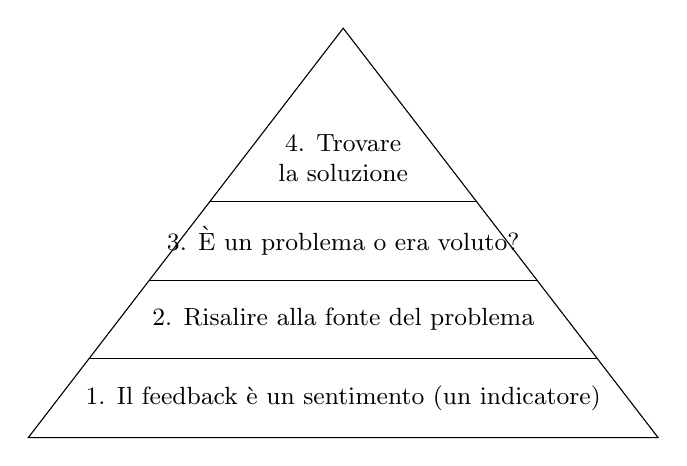
\begin{tikzpicture}[font=\small]
  \draw (0,0) -- (8,0) -- (4,5.2) -- cycle;
  \draw (0.77,1) -- (7.23,1);
  \draw (1.54,2) -- (6.46,2);
  \draw (2.31,3) -- (5.69,3);
  \node at (4,0.5) {1. Il feedback è un sentimento (un indicatore)};
  \node at (4,1.5) {2. Risalire alla fonte del problema};
  \node at (4,2.5) {3. È un problema o era voluto?};
  \node[align=center] at (4,3.55) {4. Trovare\\ la soluzione};
\end{tikzpicture}
\caption{La piramide del feedback come la descrive il relatore: si parte
dalla sensazione riferita da chi dà il feedback e si sale fino alla
soluzione. Ricostruzione schematica; la slide originale non è
disponibile.}
\label{p0:fig:piramide}
\end{figure}

\subsection{I feedback duri}

La piramide è anche un ottimo modo per \textbf{ricevere feedback in modo
professionale}, anche quelli difficili. Il relatore dà spesso feedback
\textbf{duri} ``anche per testarvi'': ``non perché sono stronzo''. Può dire
che una task è ``decente'', e dire anche tutto ciò che è sbagliato;
bisogna ricordarsi di lavorarci sopra e di \textbf{non prenderla sul
personale}. Magari sta testando la reazione, ``perché di fronte al vostro
capo in un'azienda non potete mandarlo a fanculo''.

% ---------------------------------------------------------------------
\section{La tecnica dell'iceberg}
\label{p0:sec:iceberg}

E se il problema è insormontabile? ``Allora, se il problema è
insormontabile, non esiste'', perché il relatore ha imparato la
\textbf{tecnica dell'iceberg} e la racconta ``come mi è stata spiegata''.
Non ha una base scientifica, avverte, ma a livello psicologico lo ha
aiutato molto. È una tecnica di \textbf{categorizzazione dei problemi}: non
è detto che un problema si risolva ``così'', ma la prima cosa da fare quando
lo si affronta è \textbf{descriverlo}, scriverlo in un testo, farne uno
schemino, e cercare di \textbf{classificarlo} in uno di quattro iceberg
(tabella~\ref{p0:tab:iceberg}). Se ne possono anche inventare di nuovi, per
esempio un iceberg ``basso e lungo'', che si estende per molto spazio invece
di essere largo.

\begin{table}[htbp]
\centering
\small
\begin{tabular}{@{}lp{4.4cm}p{5.4cm}@{}}
\toprule
\textbf{Iceberg} & \textbf{Che problema è} & \textbf{Come si affronta} \\
\midrule
\textbf{Alto} & Molto alto, insormontabile se lo si vuole scavalcare. &
Non lo si può prendere di petto: va \textbf{aggirato} in qualche modo. \\
\textbf{Largo} & Semplicemente molto grande, ma poco difficile. & Ci si
mette lì e \textbf{si fa fatica}. \\
\textbf{Nascosto} & Contiene situazioni problematiche, problemi nascosti. &
Obbliga a trovare il \textbf{problema reale} e a risolvere prima quello. \\
\textbf{Mostruoso} & Grande, difficile, complesso. & Richiede un
\textbf{approccio sistematico}, di solito suddividendolo in più parti. \\
\bottomrule
\end{tabular}
\caption{I quattro iceberg della tecnica dell'iceberg, come li presenta il
relatore.}
\label{p0:tab:iceberg}
\end{table}

Perché descrivere un problema con una forma ``geografica'' aiuta? Perché, se
lo si è descritto correttamente, si trova il modo di risolverlo. E, aggiunge
il relatore, la maggior parte delle volte si noterà che
\textbf{suddividere un problema in più parti} è la scelta migliore:
``splittate il problema in più parti, razionalizzate il problema''. Ed è
questo, conclude, il modo per affrontare al meglio il primo anno di AIV, o
tutti e tre.

% ---------------------------------------------------------------------
\section{Le domande finali}
\label{p0:sec:domande}

``Domande? Così recupero.'' E poi, davanti al silenzio: ``Oh, che
cavalcata! No, dai, vi prego, ditemi che avete dei dubbi''.

\subsection{A che cosa serve lo zone out?}

Una studentessa non ha capito il vantaggio dello zone out. Il relatore lo
spiega con la slide di figura~\ref{p0:fig:modi}: lo zone out
\textbf{potenzia la modalità diffusa}, e quindi la possibilità di trovare
soluzioni \emph{out of the box} che non si trovavano perché ci si
focalizzava troppo su un singolo punto. Se la soluzione è ``qui'' e ci si sta
concentrando ``qua'', non ci si arriva; in modalità diffusa il cervello vaga
e a un certo punto impatta nella soluzione. Inoltre rilassa la mente e, così
facendo, attiva il consolidamento, trasformando la working memory in
long-term memory. (Un partecipante commenta che sembra il cervello di un
personaggio di un film d'animazione\footnote{La trascrizione dice ``sembra
il cervello di Infeldo Sghetto 3'': il riferimento non è ricostruibile,
forse \emph{Inside Out}.}; ``vabbè, sì, certo, da qualche parte dovrà pure
venire fuori''.)

\subsection{La soluzione arriva sotto la doccia: e poi?}

Gabriele chiede: se finisco la giornata di lavoro con un problema aperto e
la soluzione mi viene a casa, sotto la doccia, mi rimetto a lavorare o me la
tengo per il giorno dopo? Nessuna delle due: \textbf{ci si prendono degli
appunti}. La tecnica migliore è avere sempre con sé un taccuino o il
cellulare (``non si dovrebbe fare, meglio un taccuino''). Il relatore tiene
il cellulare sul comodino: a volte, di notte, tornando dal bagno, gli viene
in mente qualcosa e se lo segna; a volte, fuori con il cane, si registra
mentre parla, e a volte si sblocca proprio parlando.

Tutto ciò che si è visto oggi, aggiunge, verrà ripreso durante il primo
anno, ma sono concetti che ``precedono il corso stesso'': durante l'anno non
c'è tempo, si fa il proprio corso. Qualcosa di neurocognitività tornerà a
narrative design e, al secondo anno, a game design, perché aiuta moltissimo
a \textbf{mappare il cervello del giocatore}, a capire come stimolarne certe
reazioni. Sarebbe bello approfondire, ma ``un po' rimane anche a voi'':
prendere le slide, approfondirle, leggerle.

\subsection{Arrivare da un'altra accademia}

Gabriele comincia direttamente dal secondo anno, avendo già fatto un anno in
un'altra accademia (``che purtroppo poi si sa com'è andata''); teme di
trovarsi spaesato non tanto per gli argomenti quanto per il metodo. Il
relatore distingue: \textbf{il metodo di studio è dello studente}; è il
\textbf{metodo di insegnamento} a essere diverso, e lo è (``senza nulla
togliere ai colleghi''): c'è un motivo per cui AIV fa nove ore di lezione a
settimana e il resto lo lascia allo studente. I consigli:
\begin{itemize}
  \item affrontare l'anno con \textbf{mentalità aperta}, senza crearsi
        pregiudizi solo perché arrivano cose diverse da quelle a cui si è
        abituati (e vale per tutti);
  \item se qualcosa non torna con l'istruzione precedente, \textbf{fare
        domande}, anche provocatorie: il relatore adora quando uno studente
        gli dice ``prof, questa cosa del viaggio dell'eroe io non la
        condivido, parliamone'' (``non vedo l'ora, davvero''), ``perché si
        apprende meglio''; avrebbe un problema se, da non professionista, si
        rifiutasse di rispondere per paura di come rispondere;
  \item ricordare che non è il metodo di insegnamento a cambiare lo
        studente: è il suo metodo di studio, ed è l'argomento ciò che si
        impara davvero, non il modo (``poi il modo aiuta molto, me ne rendo
        conto'').
\end{itemize}
Il problema vero, prevede il relatore, non sarà il metodo, ma il fatto che i
compagni hanno già un anno alle spalle e hanno affrontato cose che Gabriele
non ha visto, e su cui dovrà aggiornarsi. Il consiglio ``spassionato'':
\textbf{fare amicizia, aprirsi agli altri}. Ci si può far male, ``fa parte
del gioco''; ma essere aperti non vuol dire ``dare la propria password a
tutti'' (``a volte gli studenti mi prendono troppo alla lettera''): vuol
dire \textbf{dialogare}, e dialogare ``batte qualsiasi cosa''. Creare una
buona sinergia con la classe, cercando compromessi se serve.

\subsection{Come accorgersi di stare imparando un metodo sbagliato?}

Federico chiede come ci si accorge di stare imparando un metodo sbagliato,
per evitare il ``polso del chitarrista''. In parte sono i docenti a dirlo,
con i feedback: certe cose lo studente non può capirle da solo. Altre invece
le si nota confrontandosi con i compagni: ``cavolo, ma a me questa cosa
viene difficile, perché?''; ``mi viene, ma la sento macchinosa,
arzigogolata''. È possibile, non certo, che si stia avviando un effetto
Einstellung: si sta forse aprendo la bottiglia con una forza esercitatissima,
quando ne servirebbe molta meno.

\subsection{E all'università?}

Filippo, che frequenta anche l'università, chiede se questi metodi si
applichino a contesti più teorici, con meno possibilità di cambiare medium.
Il relatore premette di parlare ``con le pinze''. Ha fatto l'università e
``se ne pente parzialmente'': secondo lui l'università italiana ha
``tantissime competenze e conoscenze, ma pessime metodologie di
preparazione''; è soprattutto un istituto di ricerca e di studio, tranne le
facoltà pragmatiche (suo fratello è ingegnere elettrotecnico, con dottorato,
e doveva letteralmente fare circuiti; medicina è molto pratica). Ci sono
università di game design in Italia, ma con limiti: il ministero impone
esami come storia del videogioco, ``che è molto utile, ovviamente''.

Lui lavora per lo più con clienti, e al cliente non interessa la teoria né la
storia del videogioco fine a se stessa. La storia è utile \textbf{quando la si
applica}. Esempio, ripreso da ``stamattina'': il fatto che \emph{Pac-Man}
rallenti impercettibilmente mangiando i pallini\footnote{Si veda il
capitolo sul narrative design (sezione~\ref{p3:sec:mindset}). Il dettaglio
storico è che Pac-Man si ferma per un fotogramma a ogni pallino mangiato,
risultando un po' più lento dei fantasmi nei corridoi pieni di pallini.}
serve se un giorno, al lavoro, bisogna far rallentare il personaggio, senza
che il giocatore se ne accorga, quando fa certi passi, per renderlo più
raggiungibile e dargli la sensazione di ``oddio, non ce la faccio!'', magari
in una scena molto tesa di un horror: si prende la soluzione di Pac-Man e la
si adegua al contesto.

È molto importante che esista la ricerca: AIV ha bisogno degli studiosi,
il relatore lavora spesso con consulenti esperti di antropologia o di
storia. Ma non crede che un neolaureato sia pronto per l'industria, perché
molte tecniche della game industry non si insegnano all'università e
viceversa. Cita, senza nominarlo, uno studioso americano diventato un
professore importantissimo, che pubblica saggi di game design: saggi che
mostrano non un'incapacità di comprendere i framework, ma una comprensione
``in una scatola chiusa'', perché non li ha mai visti all'opera in un gioco.
È la differenza fra imparare a riparare un motore e fare davvero il
meccanico, quando le cose non sono uno a uno e vanno adattate.

Filippo precisa che la sua fatica all'università è data proprio dal ciclo
``testo, esame'', senza pratica, discussione e comunicazione. Il relatore
ribadisce che in AIV, in game design, tutte le task sono pratiche: al primo
anno su prodotti pubblicati (l'analisi del \emph{core loop} di un gioco, per
dire). All'università ci sono limiti: l'ultima volta che ha collaborato con
un ateneo gli hanno detto che il ministero impone un tetto del 30\% alle
attività di laboratorio. A lui il ciclo ``studio, studio, esame'' non
piace, perché nella vita reale non funziona così: ``il mio esame è la
pubblicazione'', che arriva dopo tre, quattro, cinque anni. Le conoscenze
generali che dà l'università sono ``imprescindibili ed enormi'', ma si
possono anche recuperare. Fa l'esempio della dizione nel doppiaggio: le
regole si assorbono, e al direttore interessa che la battuta sia detta bene;
e a volte, soprattutto gli americani, chiedono uno slang, e ``prova a
chiedere in università di farti imparare lo slang newyorkese di un
rapper''\footnote{La trascrizione dice ``addizione'' per ``dizione''. Il
passaggio è confuso, ma il senso è che certe competenze professionali si
apprendono sul campo, da altri professionisti, più che in università.}: gli
attori americani si formano facendo esperienza, andando da altri attori.

Non vuole criticare l'università: collabora con università e la rispetta. Ma
non gli piacciono quelli che, finito un corso universitario, pensano di
uscire e andare dritti a fare videogiochi. ``Io l'ho sentito sulla mia
pelle'': uscito dall'università non trovava lavoro e non capiva perché;
dieci anni dopo l'ha capito: quelle cose non le sapeva, e ha dovuto
``abbassare la cresta, fare un lavoro di umiltà e dire: ho studiato
altro''.

\subsection{Anatomia, per chi l'ha già studiata}

Una studentessa ha visto che al primo anno c'è anatomia e, avendo già fatto
tre esami di anatomia, chiede come sarà strutturato il corso. Va chiesto al
direttore di 3D art, nell'incontro dedicato (capitolo~\ref{p6:cap:3d}): il
relatore sa poco di quel corso, se non che al primo anno ci sarà una
collaborazione con i narrative per il \emph{world building} di un
gioco\footnote{Nella trascrizione: ``per il war building del giocato'',
probabilmente ``del giocattolo'': il corso di narrative prevede un modulo
di world building per i giocattoli (si veda il capitolo~\ref{p3:cap:narrative}).};
``vi diremo tutto a tempo debito'', in primavera.

\subsection{Le fiere: chi paga?}

Ultima domanda: se uno degli eventi di settore richiesti per il certificato
di eccellenza (sezione~\ref{p1:sec:eccellenza}) fosse una fiera come la
Gamescom, le spese sarebbero individuali? AIV fornisce \textbf{il biglietto
e l'alloggio} (dopo un'incertezza: ``vitto e alloggio\ldots\ scusatemi,
biglietto. No, alloggio'') ma non il trasporto, per \textbf{una fiera
all'anno}, a chi ha acquistato l'opzione \emph{Experience}; ``c'è scritto
sul sito''. La fiera la decide AIV ogni anno, sulla base di quella più
indicata; al terzo anno è al cento per cento la \textbf{First
Playable}\footnote{La trascrizione dice ``force playable''. La First
Playable è l'evento business dell'industria videoludica italiana che si
tiene a Firenze.}, ``perché alla First Playable bisogna andare''. A volte
le fiere mandano sconti, e la segreteria li comunica su Discord:
``sfruttateli assolutamente''. Ma AIV non ha la forza economica di mandare
tutti in fiera, solo chi ha l'Experience. Il relatore, che è di Milano, alla
Milan Games Week di solito scrive un messaggio per organizzare un
\emph{meet up}. La Gamescom è ``estremamente costosa'' anche da soli: chi
vuole andarci con AIV deve avere l'Experience, altrimenti si paga biglietto
e albergo. E la fiera, ogni anno, cambia.

%    % =====================================================================
%  Professioni 1 — I Dev Days: il metodo di AIV e i Dev Projects
%  Fonte: trascrizione dell'incontro di apertura dei Dev Days (AIV1):
%  un incontro online su Zoom di un'ora, il lunedì mattina della prima
%  settimana del primo anno, tenuto da Daniele Fusetto (direttore del
%  corso di narrative design e brand advisor dell'Accademia Italiana
%  Videogiochi) con Andrea Morini (direttore della didattica). Circa 31
%  partecipanti collegati su un centinaio di iscritti al primo anno;
%  slide condivise, un video di gioco senza audio, domande in chat.
%  Pacchetti richiesti nel preambolo del libro:
%    \usepackage[utf8]{inputenc}, \usepackage{booktabs},
%    \usepackage{tikz} con
%    \usetikzlibrary{arrows.meta,positioning,calc,fit}
%
%  Collocazione nel libro: parte "Alcune Professioni nel Mondo
%  Videoludico", dopo AIV0_mindset_e_best_practice (3.2).
%  Tutte le etichette di questo capitolo hanno il prefisso "p1:".
%  Il capitolo AIV0 (prefisso "p0:") rimanda a questo; questo rimanda ai
%  capitoli delle singole professioni (AIV2-AIV6).
%  La figura è una ricostruzione schematica di quanto il relatore spiega
%  con le slide, non una copia delle slide.
% =====================================================================

\chapter[I Dev Days e il metodo di AIV]{I Dev Days: il metodo di AIV,
la collaborazione fra discipline e i Dev Projects}
\label{p1:cap:devdays}

Ogni anno accademico, all'Accademia Italiana Videogiochi (\textbf{AIV}),
comincia con una settimana di incontri chiamati \textbf{Dev Days}. Lo scopo
è duplice: \textbf{impostare il lavoro} dell'inizio dell'anno e
\textbf{presentare a tutti gli studenti del primo anno che cosa faranno i
colleghi degli altri corsi}, perché, come si sentirà ripetere molte volte,
``la gaming industry è fortemente collaborativa'': i giochi si fanno in team,
e per lavorare bene con un game designer, un narrative designer, un
animatore, un programmatore o un 3D artist bisogna sapere che cosa fanno.
Questo capitolo raccoglie l'\textbf{incontro di apertura}; i capitoli
successivi raccolgono le presentazioni dei singoli corsi, cioè delle singole
professioni: game e level design (capitolo~\ref{p2:cap:gamedesign}),
narrative design (capitolo~\ref{p3:cap:narrative}), character animation
(capitolo~\ref{p4:cap:animation}), programmazione
(capitolo~\ref{p5:cap:programming}) e 3D art (capitolo~\ref{p6:cap:3d}).

A condurre l'incontro è \textbf{Daniele Fusetto}, direttore del corso di
narrative design e \emph{brand advisor} di AIV, che insegna in AIV dal 2019 e
in generale dal 2016; con lui c'è \textbf{Andrea Morini}, \textbf{direttore
della didattica}, che interviene a più riprese. L'incontro si tiene online,
su Zoom, il lunedì mattina, e dura \textbf{un'ora} (``abbiamo un'ora di tempo,
purtroppo''): non si aspetta molto chi è in ritardo, anche perché la
registrazione verrà caricata sulla piattaforma dell'accademia
(\emph{l'hub}). L'incontro non è facoltativo: ``i Dev Days non sono degli
incontri facoltativi'', bisogna almeno vederli in registrazione, ``altrimenti
si rischia di rimanere indietro fin dall'inizio''. Negli anni in cui
Fusetto e Morini hanno insegnato, ``sottovalutare una cosa del genere è di
solito il primo sintomo che qualcosa non va''.

Due avvertenze di lettura. La prima: la trascrizione è automatica e storpia
quasi sempre il nome dell'accademia (``Hive'', ``IVE'', ``Ive'', ``AIB'',
``AB'', ``IV'') e diversi titoli e termini; il capitolo usa sempre
``AIV'' e segnala in nota le ricostruzioni incerte. La seconda: molte
affermazioni riguardano l'organizzazione di AIV (calendari, regole,
certificati, opzioni di iscrizione) e valgono per l'anno a cui l'incontro si
riferisce; sono riportate come le dicono i relatori.

La data, dedotta, è \textbf{lunedì 5 ottobre 2026}\footnote{La data non è
detta. Si ricava da tre indizi: le lezioni dei corsi cominciano
``ufficialmente'' il 19 ottobre, quelle di narrative ``questo venerdì''; nel
capitolo sul narrative design, il giorno dopo, il relatore fissa la prima
lezione di narrative a ``venerdì 9 ottobre''; e nel 2026 il 9 ottobre è
venerdì. È una deduzione.}.

Il percorso del capitolo:
\begin{enumerate}
  \item l'avvio e la politica della webcam (sezione~\ref{p1:sec:avvio});
  \item che cosa sono i Dev Days e il calendario della settimana
        (sezione~\ref{p1:sec:devdays});
  \item il \textbf{metodo di AIV}: che cosa non si tollera e quattro cose da
        fare (sezione~\ref{p1:sec:metodo});
  \item \textbf{best practice} e \textbf{trappole}
        (sezioni~\ref{p1:sec:best} e~\ref{p1:sec:trappole});
  \item gli \textbf{obiettivi} dei corsi: portfolio, lavoro di gruppo,
        competenze trasversali (sezione~\ref{p1:sec:obiettivi});
  \item l'attestato di partecipazione e il \textbf{certificato di
        eccellenza} (sezione~\ref{p1:sec:eccellenza});
  \item i \textbf{Dev Projects} del secondo anno e la pipeline di sviluppo,
        con il caso di \emph{Beat of Rebellion}
        (sezioni~\ref{p1:sec:devprojects}--\ref{p1:sec:beat});
  \item perché parlarne il primo giorno, i falsi miti e le domande finali
        (sezioni~\ref{p1:sec:perche}--\ref{p1:sec:domande}).
\end{enumerate}

% ---------------------------------------------------------------------
\section{L'avvio}
\label{p1:sec:avvio}

Si comincia con qualche minuto di attesa: alcune persone sono in ritardo
``per problemi di hub'' o perché non hanno ancora fatto l'accesso. Il
relatore disabilita la sala d'attesa di Zoom e raccomanda di tenere
d'occhio il \textbf{Discord di AIV} e la propria \textbf{mail}. Poi
condivide le slide e comincia con la parte ``molto introduttiva'', mentre
arrivano gli ultimi.

\subsection{La webcam}

``Possibilmente accendete la webcam'': il relatore vuole vedere facce sveglie
``e anche le vostre camerette''. ``Mamma mia, è lunedì mattina per tutti'':
non c'è una regola che imponga di presentarsi a lezione ``belli e col volto
riposato'', ma la regola è che \textbf{ci si fa vedere}, anche quando si
segue da remoto. Non solo per buona educazione: i docenti devono vedere le
facce, le reazioni, e vogliono conoscere gli studenti anche fisicamente. Già
al tempo del COVID, ricorda, riconoscere dal vivo le persone viste online o
con la mascherina era stato ``un dramma''.

% ---------------------------------------------------------------------
\section{Che cosa sono i Dev Days}
\label{p1:sec:devdays}

L'agenda della mattina: che cosa sono i Dev Days, qual è il \textbf{metodo di
AIV}, e i \textbf{Dev Projects}, ``una cosa che voi vedrete al secondo
anno'', ma di cui i relatori vogliono dare un assaggio fin da oggi ``per
farvi capire che qua non si scherza''\footnote{La trascrizione dice
``farvi la capatanza'' e poi ``capatanta'': il senso è ``farvi fare una
capatina'', dare un assaggio. Il nome dei progetti del secondo anno
oscilla nella trascrizione fra ``Game Dev'', ``Dev Project'' e ``The
Projects''; il capitolo usa ``Dev Projects'' per i progetti e ``Game Dev''
per il percorso del secondo anno in cui si svolgono.}.

\subsection{Un'industria che lavora in team}

I Dev Days sono incontri dedicati, all'inizio del primo anno, a presentare
ciò che faranno gli altri colleghi e a impostare il lavoro. Il motivo è che
l'industria è fortemente collaborativa: \textbf{si sviluppano giochi in
team}, ``dalle 20 persone alle 400 persone''. Ci sono anche team più
piccoli, ma spesso un team di tre, quattro, cinque persone lavora molto con
\textbf{freelancer}. Esempio: si dice che \emph{Clair Obscur: Expedition 33}
sia stato fatto da trenta persone; ``non è vero, se vedete i credit, sono
400''\footnote{La cifra di 400 è del relatore. Il nucleo dello studio
Sandfall Interactive era di circa trenta persone; i titoli di coda includono
però numerosi collaboratori esterni (musica, doppiaggio, animazione,
outsourcing, localizzazione), che è appunto il punto del relatore.}. Fare
un gioco richiede un lavoro di team.

Al primo anno ognuno fa la propria disciplina: chi fa programmazione fa
programmazione, chi fa 3D fa 3D, e così per game design, character
animation, narrative design. Poi, all'inizio del secondo anno, ci si
incontrerà con tutti gli altri ``per fare insieme un videogioco''. Ma fin da
oggi bisogna capire che cosa faranno i colleghi e quali sono le altre
professioni insegnate in AIV, ``per meglio collaborare con gli altri''.

\subsection{Il calendario della settimana}

Per questo la settimana prevede \textbf{cinque incontri}, uno per ciascun
corso di AIV. Vanno seguiti \textbf{tutti}, e non sono solo per gli studenti
del corso presentato: ``sono per tutti gli studenti''. La presentazione di
game design spiega che cosa faranno i game designer durante l'anno, e la
devono seguire tutti, così che l'anno dopo, collaborando con loro, si sappia
più o meno che cosa fanno di solito. Lo stesso per narrative design,
character animation, programmazione e 3D art. L'obiettivo non è spiegare agli
studenti di quel corso che cos'è il corso (lo vedranno durante l'anno), ma
spiegare \textbf{a tutti} che cosa fanno le altre discipline. Tanto che
``probabilmente è meglio se, per esempio, la presentazione del corso di
programming la seguono più attentamente quelli che non faranno
programming''.

In più:
\begin{itemize}
  \item un incontro aggiunto quest'anno, il \textbf{giovedì mattina}, di
        un'ora e mezza, con Fusetto, anch'esso obbligatorio, sulla
        \textbf{comprensione del testo} (capitolo~\ref{pt:cap:comprensione}): ``mi spiace dirlo, ma negli ultimi
        anni ci siamo accorti che è difficile arrivare all'inizio di AIV con
        delle capacità di comprensione del testo ottime''. Non si parla di
        italiano di base né di una disciplina, ma di \textbf{comprendere
        ciò che le persone dicono e vogliono}, rispondere correttamente alle
        richieste dei docenti, evitare incomprensioni; si vedranno anche
        trucchi per comprendere meglio e per segnarsi le cose in modo da
        \textbf{saper porre domande}, ``perché è importantissimo porre
        domande'';
  \item un incontro il \textbf{martedì pomeriggio alle 14:30}, solo per chi
        si è iscritto entro il 31 luglio con la \textbf{Gamer Promo} o la
        \textbf{Dev Promo}: un incontro di \emph{mindset} e \emph{best
        practice} sulle pratiche migliori per imparare e apprendere
        durante l'anno (è il capitolo~\ref{p0:cap:mindset});
  \item per gli stessi studenti, la possibilità di una
        \textbf{mentorship} di un'ora con un tutor o un docente, ``per
        partire al meglio''. ``Sfruttatele, queste ore, perché l'anno scorso
        nessuno l'ha usata e poi dopo saltano fuori i problemi.'' Chi non
        ricorda se ha la promo può chiedere in segreteria.
\end{itemize}

% ---------------------------------------------------------------------
\section{Il metodo di AIV}
\label{p1:sec:metodo}

\subsection{In AIV si boccia}

``In AIV si boccia.'' Non è un'accademia ``dove vieni, paghi e passi
l'anno'': ci sono dei criteri. Il criterio principale è \textbf{non
consegnare le attività}, le cosiddette \textbf{task}, richieste durante
l'anno, perché la valutazione si fa su quelle: se non vengono consegnate, i
docenti non possono valutare.

Ma contano anche le \textbf{soft skill}, ``e se avete frequentato il nostro
open day lo sapete'': per passare l'anno bisogna
\begin{itemize}
  \item \textbf{interagire}: non isolarsi; chi è un po' introverso cerchi di
        uscire, di chiedere, di porre domande;
  \item \textbf{rispettare gli altri};
  \item essere \textbf{proattivi}: se viene in mente oggi che si deve o si
        può fare una cosa, non la si rimanda a domani; se si ha una domanda
        per la prossima lezione e si sa che il docente è raggiungibile per
        mail o per messaggio, non si aspetta la lezione.
\end{itemize}

\subsection{Tolleranza zero: bullismo, pregiudizi, cheating}

Su tre cose non c'è tolleranza.
\begin{description}
  \item[Bullismo.] ``Self-explanatory'', in tutte le sue forme: qualunque
        prevaricazione, anche implicita, ``non esiste''. Massima
        collaborazione e massima gentilezza, sempre.
  \item[Pregiudizi.] Si è in tanti e molto diversi, ognuno con le sue
        opinioni; ``a meno che voi non abbiate problematiche di tipo,
        diciamo, criminale, ma non credo'', bisogna partire dal presupposto
        che la persona che si ha davanti ha una sua storia, mettersi nei
        panni degli altri e \textbf{sospendere il giudizio}.
  \item[Cheating.] Fino a qualche anno fa voleva dire copiare dai compagni,
        avvantaggiarsi, manipolare la classe o i compagni per ottenere
        vantaggi non legati alla performance (``non faccio bene le attività,
        ma sono bravo a manipolare l'ambiente in modo da passare''). Negli
        ultimi due anni si è aggiunto \textbf{l'uso dell'IA}: è cheating
        quando, in un corso, viene detto di non usarla in un certo modo e la
        si usa così. Ogni corso ha il suo approccio (programmazione diverso
        da narrative, da game design, da character animation) e verrà detto
        che cosa si può fare e che cosa no. In narrative design, per
        esempio, è \textbf{severamente vietato scrivere con l'IA} per tutti
        e tre gli anni, ``vietatissimo'', fino a una lezione in cui il
        relatore spiegherà ``qual è l'unico modo, a mio parere'' per farsi
        aiutare dall'IA nell'atto della scrittura.
\end{description}

Ma cheating è anche copiare dai compagni: ``è successo, ce ne accorgiamo''.
I docenti vedono i compiti, notano forme usate nelle attività o
``spennellature, scolpiture nel modello 3D'' troppo simili. ``D'altronde, se
molti critici hanno capito che Palworld aveva copiato da Pokémon anche i
modelli 3D, si può fare''\footnote{È l'opinione del relatore, riportata
com'è. Le somiglianze fra i modelli di \emph{Palworld} e quelli dei Pokémon
sono state sostenute da utenti e commentatori dopo l'uscita del gioco
(2024), ma non sono mai state accertate; la causa intentata da Nintendo e
The Pokémon Company contro lo sviluppatore riguarda la violazione di
brevetti, non la copia dei modelli.}. Nel cheating c'è sempre una vittima,
la persona sfruttata o manipolata; ma soprattutto chi bara \textbf{fa un
danno a se stesso}: ``state pagando per imparare. Imparare voi.'' Chi usa
scorciatoie per passare l'anno e poi si ritrova senza conoscenze ha perso
un'occasione.

\subsection{Inquiry-based learning}

Poi ``quattro cose che dovete fare''. La prima: tutti i corsi di AIV sono
\textbf{inquiry-based}. ``Non esistono domande stupide, soprattutto il primo
anno.'' Molti studenti scrivono ``ho una domanda stupida'': no, non ce ne
sono. Arriva proprio in quel momento una domanda in chat (``scusi, ma i
corsi che ha fatto vedere prima sono online?''), e il relatore la usa come
esempio: ``anche qua, ragazzi, è importantissimo, \textbf{specificate bene
nelle domande}''. Si intende la \emph{lezione}, cioè il singolo incontro, o
il \emph{corso}, cioè tutto il corso? Gli incontri di questa settimana sono
tutti da remoto. Sara ha fatto una domanda ``per niente stupida'', perché
non era chiaro, ``e ha imparato anche qualcosa''\footnote{Nel capitolo sul
narrative design (sezione~\ref{p3:sec:skill}) il relatore torna su questo
episodio per spiegare perché tiene tanto alla precisione dei termini.}.
``Meno domande fate, meno imparate.''

\subsection{Un ambiente simulativo del mondo del lavoro}

La seconda: AIV è un \textbf{ambiente simulativo del mondo del lavoro}.
Tranne game programming, che ha test ed ``esamini'' (e i docenti di quel corso
spiegheranno perché), \textbf{non ci sono sessioni d'esame}, ma valutazioni
verbali tramite \textbf{task}. Durante molte lezioni, non tutte, il docente
dirà: ``voglio che mi consegniate questa task entro questa data''. Se la si
manca, la task è mancata e conta per il non passaggio dell'anno. Le task non
hanno tutte la stessa durata: in alcuni corsi sono molto corpose e
richiedono mesi; in game design e narrative sono più equilibrate, con task
da una o due settimane e altre da mesi. In sintesi: task settimanali,
mensili, trimestrali o annuali.

Bisogna entrare a poco a poco nell'ottica di un \textbf{approccio
professionale} al corso: ``prendetelo un po' come un lavoro''. Ogni giorno
si deve produrre, studiare, apprendere, confrontarsi, fare call, come in
qualsiasi lavoro, non solo nei videogiochi. La puntualità è importante;
tutti gli aspetti professionali ``in senso lato'' non sono semplicemente
graditi, ``sono mandatori''. ``Molto di più di quando i genitori ci dicevano,
alle superiori, devi pensare alla scuola come a un lavoro: questo è molto più
veritiero.'' E come nel lavoro si fanno meeting e incontri, ma si lavora
anche molto da soli: non bisogna sottovalutare il peso delle attività.

Le task sono \textbf{opportunità} per migliorarsi, ottenere più feedback e
\textbf{farsi notare dai docenti}, perché il 99\% dei docenti di AIV sono
lavoratori del settore: Fusetto stesso lavora nell'industria, sta facendo dei
giochi in questo periodo, e alcuni suoi studenti lavorano con lui. ``Non è un
modo per essere assunti'', ma permette di farsi notare per le proprie
capacità.

\subsection{Fail to learn}

La terza: \textbf{fallire}. Una delle cose più importanti da fare al primo
anno è fallire e imparare: non \emph{fail for}, ma \emph{fail to
learn}\footnote{Così nella trascrizione; il senso è ``fallire per
imparare''.}. Se si sbaglia, si ricevono feedback e si trovano soluzioni, e
piano piano si impara a trovare soluzioni ai propri fallimenti; si noterà
``un aumento notevole'' delle proprie capacità. Il consiglio pratico:
prendere una task di settembre, metterla ``in una giara virtuale'' (un
drive), lasciarla lì e a gennaio confrontarla con una task di gennaio. Se le
differenze non si notano, è perché non si è fallito e non si è imparato: ``è
una campanella d'allarme''.

\subsection{Mettere in pratica, ogni giorno}

La quarta: i corsi di AIV richiedono di \textbf{mettere in pratica} ciò che
si apprende. Perché solo \textbf{nove ore di lezione a settimana}, e non
lezioni tutte le mattine come in altre accademie? Perché bisogna avere il
tempo di mettere in pratica teoria e pratica viste a lezione: ``se io non vi
do almeno 20 ore alla settimana per mettere in pratica quello che vi insegno,
è difficile''. Il relatore porta il proprio esempio\footnote{Poco prima il relatore dice ``come diceva Andrea'': nella trascrizione i cambi di voce fra i due relatori non sono segnati, e l'attribuzione di alcuni passaggi è incerta. Qui, dal contesto (``io so programmare un pochettino'', ripetuto anche nel capitolo~\ref{p3:cap:narrative}), parla con ogni probabilità Fusetto.}: pur considerandosi un artista usa spesso Unreal Engine, e nel lavoro si acquisiscono capacità trasversali; sa
programmare ``un pochettino'', ma non ci riuscirebbe se non si mettesse
tutti i giorni quindici minuti a programmare\footnote{La trascrizione dice
``io non saprei programmare se io tutti i giorni mi mettessi lì 15 minuti a
programmare'': manca evidentemente un ``non''.}. Bisogna impegnarsi ogni
giorno nella propria disciplina. Altrimenti ci si sveglia all'ultimo, si
imparano le cose al momento del bisogno (magari anche bene), ma nasce una
sensazione di \emph{burnout}, ``e poi il burnout lo prendete''.

Quindi: mettersi da parte del tempo ogni settimana per applicare ciò che si
vede a lezione, farsi domande, fare domande ai docenti, e
\textbf{impegnarsi al massimo sulle task}. Con alcune regole:
\begin{itemize}
  \item se una task sembra \textbf{semplice}, la si fa \textbf{due volte}:
        forse si sta sopravvalutando se stessi. Se è davvero semplice, si
        chiede al docente se c'è la possibilità di avere qualcosa in più
        (``a me sembrava semplice, secondo te l'ho fatta bene?''), e magari
        arriva qualcosa di extra;
  \item se sembra \textbf{troppo difficile}, la si tenta comunque, perché
        una delle basi dell'apprendimento è l'\textbf{alternanza di
        difficoltà}: alternare task semplici e difficili fa apprendere
        meglio che fare solo le une o solo le altre;
  \item se la si finisce \textbf{in anticipo}, la si approfondisce e la si
        rifà. ``È noioso? Sì. È lungo? Sì. È pesante? Sì. Però è il
        migliore.''
\end{itemize}

\subsection{Consegnare in anticipo per avere un feedback?}

Una domanda in chat: si può consegnare una task in anticipo per ricevere un
feedback e correggere gli errori? Sì, risponde il relatore, ma con due
precisazioni. Di solito i docenti danno tutti i feedback contemporaneamente,
``perché ho bisogno di vedere anche il confronto con la classe''; si può
però mandare una task e fare \textbf{domande specifiche}. E bisogna
aspettarsi che i docenti non rispondano direttamente: a lui capita spesso
che gli chiedano ``Daniele, secondo te questa cosa l'ho spiegata troppo?
l'ho fatta troppo così?'', e lui risponde ``secondo te l'hai fatta
troppo?''. ``Non frustratevi per questo'': deve insegnare in qualche modo ad
andare avanti da soli. Non è detto quindi che si ottenga una risposta, ma si
avranno indicazioni, e chi consegna uno o due giorni prima può ricevere
feedback aggiuntivi. Una condizione: se si consegna in anticipo, deve
essere perché si è dato il massimo, non perché si è ``tirato via'' per
consegnare prima. E non è banale: nella sua carriera, ``ma anche
attualmente'', quasi nessuno riesce a consegnare in anticipo.

% ---------------------------------------------------------------------
\section{Best practice}
\label{p1:sec:best}

Le \textbf{best practice}, ``soprattutto per chi segue in remoto''.

\paragraph{Camera sempre accesa.} Vale per chi segue da remoto, ma anche per
chi segue in presenza e capita di seguire una lezione online. E capiterà:
``in Italia abbiamo una maledizione, si chiamano scioperi''. Spesso il
venerdì ci sono scioperi di mezzi, treni, autostrade, a Roma e a Milano
(``l'anno scorso Milano è stato un delirio''); per non perdere la lezione,
se c'è sciopero e il docente non può venire in presenza, la lezione del
venerdì si trasforma in lezione da remoto. In quei casi la camera va tenuta
accesa: al docente serve per vedere i volti (``vedo il volto di Mattia, di
Gabriele, di Emanuele, di Davide, vedo come sono messi, se stanno capendo
oppure no''), e allo studente è ``una scusa in meno per distrarvi'', perché
``la distrazione è sempre dietro l'angolo''.

\paragraph{Prendere appunti.} Cartacei o digitali, non importa. Non bisogna
fare come i camerieri, che pensano di prendere gli ordini a mente e
puntualmente se li dimenticano; il fenomeno ha anche un nome, l'\textbf{effetto
Zeigarnik}, ``se volete potete andarlo a cercare''\footnote{La trascrizione
dice ``Zygarnik Effect''. L'effetto è ripreso e discusso nel
capitolo~\ref{p0:cap:mindset} (sezione~\ref{p0:sec:memoria}).}.

\paragraph{Interagire con i docenti.} Fare domande durante le lezioni.

\paragraph{Rivedere le registrazioni.} Soprattutto per gli
\textbf{studenti lavoratori}. Ogni settimana ci sono nove ore di lezione; chi
lavora e sa che ne perderà tre a settimana ha il compito ``tassativo'' di
recuperarle nel weekend. Altrimenti la settimana dopo diventano sei, poi
nove, ``e improvvisamente quelle tre ore diventano 18''. ``Io ho studenti che
arrivano a giugno e mi dicono: prof, devo ancora recuperare lezioni di
febbraio. E io non rido'', perché le lezioni sono spesso consequenziali. Il
sistema di registrazione dà pochi problemi: entro 24 ore circa le
registrazioni sono disponibili (``scongiurando bug e problematiche di
cloud''). ``Guardatevele, riguardatevele, mettete il 2x piuttosto.''

\subsection{Quanto restano le registrazioni, e a che cosa servono}

A una domanda in chat uno dei relatori risponde che le registrazioni restano
attive almeno fino all'inizio dell'anno successivo, verso fine settembre,
quando si cominciano a staccare le vecchie per fare spazio al nuovo anno.
Si possono quindi recuperare anche d'estate: chi, per motivi di lavoro, non
ha consegnato abbastanza e ha bisogno di tempo per recuperare, lo ottiene
durante l'estate, con l'accesso alle lezioni.

Le registrazioni, aggiunge Fusetto (richiamando un'osservazione di Morini), servono anche ad altro: ci
saranno cose che non riescono, problemi che non si risolvono, cose non
capite. È vero che i docenti sono facilmente raggiungibili su Discord, ma
quella è \textbf{l'ultima chance}: bisogna imparare a \textbf{risolvere i
problemi da soli}. Se è qualcosa trattato a lezione, si riguarda la
registrazione, si chiede ai colleghi, si guardano gli appunti e le
dispense; si chiede a Google (``non riesco a installare questa cosa''), si
chiede ``alla maledettissima intelligenza artificiale''. Solo se nulla di
tutto questo aiuta, perché il problema è particolarissimo, si va dal
docente. Bisogna sforzarsi di non avere ``la pappa pronta'': fa parte del
\emph{problem solving}. È come con un datore di lavoro: non si va dal capo a
ogni problema, prima si cerca di risolverlo. Al primo anno, precisa
Fusetto, va bene scrivere qualsiasi domanda quando si vuole (e così per gli
altri docenti, secondo le indicazioni che daranno); al secondo anno
comincerà a dire ``guarda che per questa cosa potevi anche non scrivermi'',
perché nel lavoro non si può scrivere al capo ``ogni due per tre''.

Chi ha bisogno di ancora più tempo ha l'opzione \textbf{Companion},
acquistabile anche durante l'anno accademico, che dà accesso alle lezioni
per un altro anno: è pensata per chi ha davvero bisogno di più tempo, e
richiede un processo dedicato (le lezioni vengono spostate su un altro
server), con più tempo, costo e lavoro. ``Non è un obbligo, ovviamente.''

% ---------------------------------------------------------------------
\section{Trappole}
\label{p1:sec:trappole}

Poi le \textbf{trappole}, ``trappoloni''.

\paragraph{``Mi basterà ascoltare?''} Molto spesso no.

\paragraph{``Posso fare altro nel mentre?''} ``Altro trappolone enorme, che
l'anno scorso ha fatto cadere tantissime persone'': ``tanto sono indicazioni
di massima, poi mi rivedo la lezione''. No. Andrea Morini, ``come direttore
didattico, terribile'', avverte che i docenti sanno se, durante una lezione
da remoto, qualcuno guarda una serie TV o gioca; e ci sono stati studenti
che giocavano in aula mentre il docente spiegava. ``Non è ammissibile in
nessun caso, mai'': a quel punto interviene lui, ``io sono quello cattivo''.
Massima attenzione: \textbf{nessuno è multitasking}, ``è falso''. Si segue la
lezione e basta, si spegne il cellulare. Anche perché seguire più cose
contemporaneamente \textbf{affatica}, anche se non sembra.

\paragraph{``Farò due minuti di ritardo, che sarà mai?''} C'è un ritardo
ammesso di 5--10 minuti, ma \textbf{non c'è il quarto d'ora accademico},
a meno che il docente non lo conceda. Se il docente dice ``10:10 in aula'' o
``14:10 in aula'', a seconda dell'orario, o ``questo orario, \emph{sharp}'',
bisogna essere puntuali.

\paragraph{``Sono come tutorial.''} ``Questo è un grande altro tema'': il
trappolone del ``tanto è come un tutorial di YouTube, poi me lo seguo in
registrazione''. No: rispetto a un corso su YouTube, su Udemy o a un corso di
formazione registrato, si ha un vantaggio, \textbf{si può chiedere
direttamente al docente}, che è un esperto del settore (``nel corso di Udemy,
vi posso assicurare, non sapete chi è il docente''). Anche quando una
lezione è un tutorial, ``non è davvero un tutorial'': si può chiedere di
rispiegare. E, ricordando le soft skill (niente pregiudizi, rispetto), se un
collega chiede ``prof, può rispiegare?'' e noi avevamo capito, anche se
pensiamo di annoiarci, conviene pensare ``magari mi sono perso comunque
qualcosa''. ``Non è un errore rispiegare, anzi, molto meglio rispiegare.''

% ---------------------------------------------------------------------
\section{Gli obiettivi dei corsi}
\label{p1:sec:obiettivi}

\subsection{Obiettivi primari: portfolio, problemi reali, lavoro di gruppo}

Il primo obiettivo, tutto l'anno e tutti gli anni, è \textbf{lavorare per
realizzare un portfolio}. Oltre al ``pezzo di carta'', la cosa principale per
entrare nella game industry è il portfolio: i giochi creati, i prodotti
fatti, i modelli 3D per i 3D artist, il software per i programmatori, gli
script per i narrative designer, le task per i game designer, le animazioni
per i character animator.

Attenzione, ``soprattutto programmatori e 3D artist, che di solito
sottovalutano questo punto'': \textbf{i giochi pubblicati sono l'elemento di
portfolio più importante di tutti}, più degli altri giochi fatti e ancora di
più delle task. Quando un selezionatore delle risorse umane, ``ma soprattutto
un lavoratore di un'azienda videoludica'', valuta un portfolio, considera più
importanti i giochi pubblicati su itch.io o su Steam, anche con gli amici
per una jam (non devono essere tripla A, devono essere accessibili), di
qualsiasi elemento legato a giochi mai pubblicati. ``Ho fatto un modello 3D.
È stato pubblicato in un gioco? No? Vale di meno'', e vale ancora meno della
task. Per questo, andando avanti negli anni, bisognerà riuscire sempre di più
a realizzare giochi, e giochi pubblicati; e qui AIV aiuta con i Dev Projects.

Il secondo obiettivo è lavorare su \textbf{problemi e progetti reali}: c'è
``un implicito accordo'' fra docenti e studenti per cui i docenti danno
problemi che davvero si troveranno nell'industria, quelli che si affrontano
tutti i giorni. E il terzo è lavorare \textbf{in gruppo} per potenziare le
soft skill. ``Fondamentale'': bisogna creare fin dai primi mesi un
\textbf{ottimo corpo classe}, una buona sinergia fra studenti. Secondo i
numeri e le analisi di AIV (``e Andrea ve lo può confermare''), le classi
molto unite, con studenti che si supportano, hanno molte più possibilità e
meno problemi di quelle che litigano. ``È banale da dire'', eppure non si sa
quante volte micro faide e micro litigi nati per niente creino problemi
``atroci, enormi''.

Andrea Morini aggiunge che queste cose derivano spesso da una sbagliata
considerazione del proprio \textbf{ego}: ``qui non c'è ego''. Non vuole
vedere nessuno che, per motivi di ego, rallenti o danneggi i colleghi,
anche involontariamente, senza accorgersene e senza malizia, ``ma succede''.
``Qui l'ego lo potete mettere da parte, e allora andiamo tutti d'accordo.''

\subsection{Obiettivi secondari: competenze a T rovesciata}

Fra gli obiettivi secondari ci sono le \textbf{competenze a T
rovesciata}\footnote{La trascrizione dice ``competenze ti è rovesciata'' e
``competenza tirovesciata''. Il riferimento è al modello delle competenze
``a T'' (\emph{T-shaped skills}): una competenza profonda in una
disciplina (l'asta verticale) unita a una conoscenza più ampia delle
discipline vicine (il tratto orizzontale). Il relatore lo chiama ``a T
rovesciata'', con il tratto orizzontale alla base.}. Nell'industria si torna
a parlare del fatto che stanno tornando lentamente i \textbf{generalisti}.
È un ciclo costante dagli anni Settanta, da quando sono nati l'informatica e
il software: le industrie tecnologiche preferiscono, alternativamente,
persone con competenze variegate che sanno lavorare su tutto un prodotto (i
cosiddetti \emph{full stack}: programmatore full stack, game designer full
stack) oppure persone molto specializzate, \textbf{verticali}. Fino a prima
dell'IA era molto importante essere ``terribilmente verticali''; proprio in
questi giorni Fusetto e Morini si sono confrontati sul fatto che molte
aziende cominciano a pensare di tornare indietro e avere generalisti,
perché con l'IA c'è ``questa sorta di verità e illusione'' (``lo sapremo
solo con calma nel tempo'') che una persona con competenze differenti
funzioni di più.

AIV insegna a T rovesciata, e questo mette gli studenti in una sorta di
``bunker protettivo'': i corsi sono verticali, ma dentro la propria
verticalità si vedono tante cose. In game design si è verticali sul game
design, ma si vede Unreal, si programma con i Blueprint, si fa level design,
combat design: ``vedete tutto quello che c'è nel game design''. E nessuno,
nell'industria, chiederà a un game designer di fare modelli 3D: magari
competenze di base per mettere gli asset nell'engine, ``ma non vi potrete
sostituire a un modellatore 3D''. Bisogna quindi essere
\textbf{intraprendenti}: imparare tutte le sfaccettature del proprio lavoro
e, al secondo e terzo anno, nei lavori di team, imparare anche \textbf{per
osmosi} da ciò che fanno i colleghi.

Andrea Morini aggiunge un dettaglio: AIV ``si mette sempre in discussione''.
Un paio di volte l'anno va a vedere ``non so quante'' \emph{job
description}, le posizioni aperte, per verificare quanto sia vero che il
generalista sta tornando di moda: ``poco, poco''. Oggi le posizioni aperte
sono ancora ``estremamente verticali, non se ne esce''; nei piccolissimi
studi di tre o quattro persone un generalista può essere più apprezzato,
altrimenti no. Quindi, all'uscita, ci si propone come \textbf{specialisti
della propria disciplina}, e in azienda scopriranno che si sa fare anche
altro. Spesso si entra con una qualifica e si esce con un'altra (magari si
entra in un ruolo junior di base, ``adesso poi dovremo vedere che cosa
succederà con le posizioni junior''), e nulla vieta di fare carriera
all'interno.

\subsection{Competenze spendibili fuori dal settore}

Le competenze sono importanti anche per l'\textbf{extrasettore}: in tutti i
corsi si imparano cose spendibili anche fuori dalla game industry, e questo
serve per due motivi. Se non si trova lavoro nell'industria, si possono usare
altrove; e se dopo tre anni ci si convince che quello non è il proprio
futuro, idem. Fusetto ha ``moltissimi studenti'' che hanno cambiato carriera
usando le competenze acquisite. Si augura che tutti facciano il lavoro per cui
si sono iscritti, ma ``non abbiamo la palla di cristallo'': meglio prevenire
che curare.

Al terzo anno, inoltre, si fanno molte lezioni, anche con i \textbf{Career
Days}, sulle \textbf{competenze imprenditoriali} e sul
\textbf{freelancing}: non c'è solo l'assunzione in azienda, c'è il freelance
(Fusetto è freelancer) e c'è chi vuole aprire un'azienda. L'Italia, dice,
ha due cose ``fenomenali'': la capacità degli italiani di essere imprenditori
e di sognare in grande, e ``la stragrande capacità del governo italiano di
mettere burocrazia per impedire l'imprenditorialità''. Sulla burocrazia non
si può lavorare, ma si può diventare intraprendenti, evitare errori enormi e
diventare imprenditori migliori, ``per esempio degli americani'': un
americano apre una società in due ore con una carta di credito e al primo
problema si blocca; un italiano dice ``che sarà mai, ho passato ore
chilometriche a fare burocrazia''.

% ---------------------------------------------------------------------
\section{Attestato di partecipazione e certificato di eccellenza}
\label{p1:sec:eccellenza}

La parte sui certificati la presenta Andrea Morini. Da qualche tempo AIV ha
introdotto l'\textbf{attestato di partecipazione}, che attesta che si è
partecipato al corso, cioè che si è fatto ciò che il corso richiede:
\textbf{consegnare le task}. Non basta essere stati presenti (``è implicito
che è importante''); è ancora più importante \textbf{produrre}, così da potersi
confrontare su ciò che si produce.

Accanto c'è il \textbf{certificato di eccellenza}\footnote{La trascrizione
dice ``il CTV Audi Eccellenza'' e ``il certificato di scelta'': si tratta in
entrambi i casi del certificato di eccellenza.}, per chi dà importanza a
tutto ciò che si sta dicendo e applica queste best practice. I requisiti
sono tre:
\begin{enumerate}
  \item \textbf{aver prodotto molto e bene}: essere promossi, aver
        consegnato \textbf{tutte} le task dell'anno (``per alcuni corsi sono
        tante'') e superato gli eventuali test; oppure aver consegnato
        \textbf{almeno l'80\%} delle task, ma con \textbf{metà di questo 80\%
        valutata eccellente}, a discrezione del docente;
  \item \textbf{aver partecipato ai Dev Projects}, collaborando fino al
        \textbf{completamento} del progetto (non necessariamente alla
        pubblicazione); se per qualsiasi motivo non è stato possibile
        (``non perché lavorate, non potete'', ma perché il progetto è stato
        chiuso perché non andava bene, ``mille motivi''), aver partecipato
        almeno a delle \textbf{game jam}: ``è il \emph{second best}'';
  \item aver partecipato \textbf{almeno a un secondo evento di settore}
        ogni anno, oltre alla jam: ``sembra che dobbiamo metterla come un
        premio, e invece dovrebbe essere la prassi''.
\end{enumerate}

Gli eventi di settore sono fondamentali soprattutto per il
\textbf{networking}: crearsi una rete di conoscenze nell'industria che, in
futuro, ``probabilmente mi agevolerà'' nel trovare lavoro. Va fatto da
subito, non alla fine del corso: le game jam sono un modo, gli eventi di
settore (AIV ne indicherà alcuni; sulla slide ce ne sono degli esempi) sono un
altro. ``Dovete farlo''; AIV lo riconosce con il certificato. ``Dovreste
farle a prescindere, però se le fate a noi piace, tra virgolette, premiarvi
con un bollino di eccellenza.''

Il certificato ha un valore anche nel curriculum. Come Morini ha spiegato
``anche ieri all'open day'', quando si selezionano persone per un lavoro si
fa una prima scrematura cercando almeno un certificato di scuola, università
o accademia equiparata (``non importa laurea o non laurea, all'estero''):
l'importante è aver fatto un percorso dopo le superiori. Poi si guarda il
portfolio, ma si guardano anche i \textbf{meriti}. Il certificato di
eccellenza è ``un'ottima occasione per brillare''.

% ---------------------------------------------------------------------
\section{I Dev Projects}
\label{p1:sec:devprojects}

``Cerchiamo di correre verso la fine, abbiamo ancora un quarto d'ora
circa.'' ``Voi siete qua perché volete fare giochi, giusto? Quindi
facciamoli.''

\subsection{Che cosa sono}

Come si fa un gioco? Di solito ci sono tre fasi, mutuate dal cinema:
\textbf{pre-produzione}, \textbf{produzione}, \textbf{post-produzione}. Da
questo metodo AIV prende il modello di sviluppo del secondo anno.
All'inizio del secondo anno, dopo i \emph{pressure test} e i test di inizio
anno, quindi intorno a novembre (quest'anno il \textbf{18 novembre}), gli
studenti del secondo anno vengono divisi in \textbf{gruppi
interdisciplinari}, che devono fare il \textbf{pitch} di un gioco da
sviluppare nei \textbf{due anni} successivi. I migliori vengono pubblicati.

Si chiamano \textbf{Dev Projects} e sono ``sviluppo ludico reale in contesto
didattico'': a AIV non piace chiamarli progetti studenteschi, ``perché non
lo sono''. Sono supervisionati da un comitato di esperti (``una
controlunca'' nella trascrizione), di cui fa parte anche Fusetto, dal
concept alla release. I migliori vengono pubblicati ``live'' su
\textbf{Steam} e su \textbf{Epic Games Store}: dall'anno scorso, dice il
relatore, AIV è diventata una delle tre accademie in Europa, e l'unica in
Italia, a poter pubblicare i giochi degli studenti su Epic\footnote{È
un'affermazione del relatore, non verificata.}.

``Pubblicati'' non vuol dire messi online per amici e parenti: sono
prodotti \textbf{gratuiti} che vengono scaricati \textbf{fra le 60.000 e le
100.000 volte}; \emph{Steam Rush} è stato giocato da 100.000 persone; le
recensioni medie vanno da ``positive'' a ``molto positive''. ``Non stiamo
parlando di piccoli giochi che fate nel giardino di casa'', ma di prodotti
che possono fare la differenza fra essere assunti o no: molti degli autori
di \emph{Steam Rush} sono stati assunti proprio perché l'avevano nel
portfolio.

\subsection{I giochi pubblicati}

Una slide mostra i giochi pubblicati finora (``da aggiornare'').
L'elenco, nella trascrizione, è in buona parte storpiato\footnote{La
trascrizione riporta: ``l'Eder, il Beautiful, il Duality Shift \ldots\ Tito
Rebello e Duality Shift sono già stati pubblicati. Powerful viene
pubblicato a breve. Solarpunk e D'Angelo Augusto avranno una storia un po'
più lunga. Operation Remote, Bolbuletti e Steamrash sono già fuori. Gunpire
e Ancora For Atlanti \ldots''. ``Tito Rebello'' è con ogni probabilità
\emph{Beat of Rebellion}, il gioco mostrato subito dopo; gli altri titoli
non sono ricostruibili con certezza e sono riportati come appaiono.}: fra i
titoli riconoscibili ci sono \emph{Beat of Rebellion}, \emph{Duality
Shift}, \emph{Operation Remote} e \emph{Steam Rush}, già usciti; un altro
uscirà a breve; due progetti ``avranno una storia un po' più lunga''. Due
giochi, \emph{Gunpire} e un altro, sono stati anche \textbf{finalisti al Game
Development World Championship 2025}.

\subsection{Perché sono importanti}

Perché parlarne già adesso, un anno prima? Perché i Dev Projects sono ``la
vostra chance principale per lavorare in questa industria''. ``Voi siete qua
per fare giochi, dimostratelo'': dimostrare di saper lavorare in team, di
superare problemi interpersonali, di capire come lavorano gli altri
dipartimenti, di costruire un portfolio, di lavorare in modo simulativo
del mondo del lavoro.

Alla fine del terzo anno, insieme al certificato di partecipazione, AIV
consegna \textbf{la custodia del gioco} con dentro la scheda SSD o la chiave
USB con la \emph{build} (``non c'è la slide, ma la dovrei mettere''): per far
capire di aver fatto una scuola che ha fatto realizzare un prodotto reale. I
giochi vengono poi pubblicati \textbf{nei 6--8 mesi successivi} al terzo
anno, durante i quali AIV continua a seguire gli studenti
\textbf{gratuitamente}: Fusetto e \textbf{Giacomo Caneschi}, direttore di 3D
art (capitolo~\ref{p6:cap:3d}), seguono i prodotti e lo sviluppo ``perché ci
piace che i nostri studenti pubblichino''.

% ---------------------------------------------------------------------
\section{La pipeline di sviluppo}
\label{p1:sec:pipeline}

Come avviene lo sviluppo? Saperlo serve già al primo anno, perché molti
faranno progetti nella propria classe. La pipeline mostrata è questa
(figura~\ref{p1:fig:pipeline}):
\begin{description}
  \item[Pre-produzione.] Un \textbf{concept}, un \textbf{vision document},
        una fase di \textbf{ricerca}.
  \item[Vertical slice.] ``Un prototipo prototipato''\footnote{Così nella
        trascrizione: il senso è un prototipo rappresentativo del gioco
        finito, completo in una sua piccola porzione.}.
  \item[Produzione.] Design, development, prototipo.
  \item[Release candidate.] Il candidato al rilascio. Un tempo, dice il
        relatore, nell'industria si chiamava \emph{Release to Market},
        perché era la build che si metteva nei CD; oggi che molti giochi
        sono pubblicati in digitale si chiamerebbe \emph{Release to
        Marketing}, la build consegnata al marketing per la
        promozione\footnote{La sigla in uso nell'industria del software è
        RTM, \emph{Release to Manufacturing}: la versione consegnata alla
        produzione fisica dei supporti. ``Release to Market'' e ``Release to
        Marketing'' sono le espansioni date dal relatore; la seconda, in
        particolare, sembra una sua interpretazione.}.
  \item[Polishing, marketing, community management.] Chi segue, come il
        relatore, \emph{Control Resonant} può vedere quanto marketing si
        sta facendo per spingere il gioco: ``tantissimo''.
  \item[Customer care.] Un gioco è un software, e serve assistenza al
        cliente: magari un cliente l'ha comprato ma non riesce a
        scaricarlo.
\end{description}
Un gioco, insomma, non finisce al rilascio: ci sono i DLC, ci sono le patch.
``Il \emph{Control} è già stato patchato tre volte, siamo alla 1.4, è uscito
da una settimana''\footnote{La trascrizione dice ``il controverso è già
stato patchato'': dal contesto è \emph{Control Resonant}, citato poco prima.
I dettagli sulle patch sono quelli riferiti dal relatore.}. ``C'è da
lavorare anche dopo.''

Una precisazione terminologica, valida per tutto l'anno: ``io parlo in
termini tecnici, se non è chiaro, chiedete''. Per \textbf{build} si intende
l'eseguibile del gioco, il file \texttt{.exe} che si può cliccare e lanciare
(per esempio da Steam); più in generale, la build è \textbf{la versione del
gioco su cui si sta lavorando}.

\begin{figure}[htbp]
\centering
\begin{tikzpicture}[
  fase/.style={draw, rounded corners, align=center, font=\footnotesize,
               minimum height=1.25cm, text width=2.05cm},
  >=Stealth, node distance=0.35cm]
  \node[fase] (pre) {\textbf{Pre-produzione}\\ concept, vision,\\ ricerca};
  \node[fase, right=of pre] (vs) {\textbf{Vertical\\ slice}};
  \node[fase, right=of vs] (prod) {\textbf{Produzione}\\ design, sviluppo,\\ prototipo};
  \node[fase, right=of prod] (rc) {\textbf{Release\\ candidate}};
  \node[fase, right=of rc] (post) {\textbf{Post-produzione}\\ polishing, marketing,\\ community, assistenza};
  \draw[->, thick] (pre) -- (vs);
  \draw[->, thick] (vs) -- (prod);
  \draw[->, thick] (prod) -- (rc);
  \draw[->, thick] (rc) -- (post);
  \draw[->, thick, dashed] (post.south) -- ++(0,-0.6) -| node[pos=0.25, below, font=\scriptsize]
       {patch, DLC: il lavoro continua dopo il rilascio} (prod.south);
\end{tikzpicture}
\caption{La pipeline di sviluppo dei Dev Projects come la presenta il
relatore. Ricostruzione schematica.}
\label{p1:fig:pipeline}
\end{figure}

% ---------------------------------------------------------------------
\section{Un caso: l'evoluzione di \emph{Beat of Rebellion}}
\label{p1:sec:beat}

Per far vedere come cambia un gioco lungo la pipeline, il relatore mostra
\emph{Beat of Rebellion}, uno dei giochi pubblicati l'anno precedente.
\begin{itemize}
  \item \textbf{Pre-produzione.} I bozzetti, il \emph{concept document} e
        una ``build ipotetica'', il prototipo realizzato nella fase di
        ricerca\footnote{La trascrizione dice ``la GIM che avevano nella fase
        di ricerca'': la parola non è ricostruibile; dal contesto si tratta
        della build prototipale di quella fase.}.
  \item \textbf{Vertical slice.} Dopo circa sei mesi, da gennaio a giugno,
        la vertical slice. La slide mostra il \emph{level design} visto
        dall'alto: ``non è così il gioco'', che è isometrico e segue il
        personaggio.
  \item \textbf{Produzione.} Il lavoro sul livello: il livello c'era già,
        ma è stato annotato, è stato sviluppato il personaggio e l'aspetto
        grafico. Si vede il livello crescere, e si nota la differenza a
        livello di \textbf{texturing}: un modello 3D senza texture, cioè
        senza quell'aspetto di superficie, e lo stesso modello con la
        texture. ``Queste parole imparatele tutti, non solo i grafici 3D.''
        È stato fatto anche \emph{character development} degli NPC.
  \item \textbf{Release candidate.} Ciò che hanno prodotto alla fine del
        terzo anno, quando i supervisori hanno detto ``potete pubblicarlo
        entro fine anno'': non è la versione pubblicata su Steam, ``che è
        ancora meglio'', e ha ancora qualche piccolo bug. Si vede che lo
        stanno giocando dall'editor di Unreal, perché il personaggio lascia
        delle scie, dei \emph{ghost}, legati ai test in corso. ``Ma guardate
        questa camera che fa vedere il livello'': non sono cose che si vedono
        di solito in un gioco di studenti, ``perché questo non è un gioco di
        studenti''. Fare le camere, le animazioni, capire come fare il salto,
        il doppio salto, il \emph{dash}: tutte cose che si vedranno durante
        gli anni.
  \item \textbf{Post-produzione.} Polishing, marketing, miglioramento della
        pagina del gioco ``a livello di SEO'', fatto con il relatore: per un
        periodo, ``forse anche adesso'', cercando il titolo il gioco usciva
        come primo risultato, ``c'è tutta una tecnica per farlo''. Sono
        state migliorate anche le \textbf{icone} dei poteri dei personaggi,
        che prima erano ``semplicemente abbozzate''.
\end{itemize}
Il video è senza audio (``no, non funziona l'audio''), ``ed è un peccato,
perché è un gioco che si basa sul beat'', sulla musica. ``Cercatelo online,
giocatelo'': è migliorato tantissimo.

% ---------------------------------------------------------------------
\section{Perché parlarne oggi}
\label{p1:sec:perche}

Perché dirlo il primo giorno? Perché si è qui per fare videogiochi, che sia
entrando nell'industria, come sviluppatori indipendenti o come freelance:
se si vogliono fare giochi, i Dev Projects ``sono il vostro futuro''. Di
più: al secondo e al terzo anno Fusetto obbligherà a fare le \textbf{jam},
come la \emph{Fast Starter Jam} di inizio anno\footnote{Nel
capitolo~\ref{p2:cap:gamedesign} la stessa jam è chiamata ``Firestarter''; il
nome esatto non è ricostruibile con certezza.}, ``perché voi dovete fare
giochi'': si deve uscire da AIV con \textbf{almeno due o tre giochi
pubblicati} su itch.io o su Steam.

C'è un anno prima di cominciare i Dev Projects, e in quell'anno si può
perdere entusiasmo. Il relatore vuole far capire \textbf{perché} lo si fa,
così da arrivare al secondo anno con l'entusiasmo di oggi: chi oggi non ha
l'\emph{hype} del ``io voglio farlo, quel videogioco'' non sopravviverà al
secondo anno. Bisogna mantenere l'entusiasmo: ``occhi sulla meta, come si
dice in America''.

Che cosa fare quest'anno per prepararsi al meglio?
\begin{itemize}
  \item \textbf{comprendere meglio la propria disciplina}: il primo anno si
        imparano le basi;
  \item essere \textbf{aperti a punti di vista} diversi;
  \item lavorare sul \textbf{mindset}, soprattutto su come prendere e
        recepire i \textbf{feedback}: introspettarli, farli propri, usarli,
        capirli;
  \item cominciare a \textbf{stringere amicizie} nel settore partecipando
        agli eventi, che di solito vengono comunicati sul Discord di AIV
        (ci sono chat dedicate; spesso AIV stessa viene invitata come
        accademia); ma anche informarsi da soli, scrivere, andare online:
        ``non siate passivi, siate proattivi''.
\end{itemize}

% ---------------------------------------------------------------------
\section{Falsi miti e cose a cui stare attenti}
\label{p1:sec:miti}

Le ultime slide, ``rapide'', elencano alcuni falsi miti.
\begin{description}
  \item[``Non mi serve il Dev Project, ho un portfolio da scrittore o da 3D
        artist.''] \textbf{Il gioco pubblicato batte tutto.} Nazareno
        Urbano, amico del relatore e \emph{principal environment artist} in
        Remedy, ha detto in più interviste: ``la prima cosa che guardo in un
        3D artist è quanti giochi ha pubblicato e quali. Poi il portfolio,
        ma prima guardo i giochi''.
  \item[``Posso ghostare gli altri membri del team, tanto chi se ne
        frega.''] No: si rispetta l'impegno degli altri. Se ci si dà un
        appuntamento con i compagni a una certa ora, ci si va: ``questa non
        è una scuola superiore, questa è un'università''. Si comunica fra di
        sé.
  \item[``Posso operare in autonomia.''] No: si coinvolge il team.
  \item[``Facciamo un open world MMO online multiplayer.''] No: ``fate il
        passo lungo quanto la gamba''. Niente prodotti troppo grandi: ``non
        siete qua per fare il nuovo Pokémon''; per quello servono soldi,
        tempo e persone. Bisogna pensare giochi \textbf{realizzabili in due
        anni}. Vale anche al primo anno, ``perché anche quest'anno farete
        cose''.
  \item[``Non serve la documentazione, non serve tenere traccia delle
        decisioni.''] Vale anche per chi fa progetti al primo anno: ``tanto
        non serve scrivermi come ho fatto''. Serve, ``perché se no fate un
        buco nell'acqua ogni volta''. La documentazione si fa.
  \item[``Lo facciamo quando abbiamo tempo.''] No: bisogna
        \textbf{programmarsi la giornata}, ``programmatevi la vostra
        vita''. La gestione del tempo e delle task è fondamentale e fa
        parte delle soft skill: tutte quelle capacità non tecniche di
        gestione, di \textbf{autogestione}, di rapporti interpersonali.
        ``Anche lavorare su se stessi è fondamentale.''
\end{description}

% ---------------------------------------------------------------------
\section{Chiusura e domande}
\label{p1:sec:domande}

L'ultima slide invita a sfruttare gli \textbf{eventi Growth}\footnote{È il
nome, nella trascrizione, della serie di incontri di inizio anno di cui fanno
parte i Dev Days.} per capire come lavoreranno i colleghi e ragionare sulle
altre discipline: partecipare, o almeno vedere le registrazioni. Oggi sono
collegate \textbf{31 persone su 100}: ``è un terzo, è pochissimo''; l'anno
scorso erano almeno la metà. Il relatore si aspetta di vederne almeno una
cinquantina il giorno dopo, alla presentazione di narrative design. Le slide
verranno mandate il prima possibile, caricate sulla piattaforma o inviate
in altro modo, a volte in PDF su Discord.

\subsection{RAM: 16 o 32 GB?}

Una domanda ``off topic'': uno studente ha un PC con 16 GB di RAM e uno slot
libero; conviene montare un altro banco da 16 per arrivare a 32? ``Che corso
fai?'' Game design. ``Direi di sì.'' Più o meno tutti i corsi usano Unreal
Engine, non nella stessa misura, e Unreal è ``molto pretenzioso, anche
troppo''. Il consiglio è di non stare sotto i 16 GB e di andare sui 32,
``senza fretta, però'', nell'arco dei prossimi mesi; ``c'è Natale'',
scherzano i relatori, e un banco di RAM ``oggigiorno è un ottimo regalo'' (non
è semplice trovarle: ``ormai sono firmate Morellato, le RAM''). Fusetto
aggiunge che 16 GB ancora reggono, ma 32 sono il minimo; lui, per portarsi
avanti, ne ha 64, ``non è obbligatorio, però non si sa mai''.

\subsection{Il colloquio personale e la modalità playtest}

``Potete anche usare il microfono, non è vietato, non abbiate paura.'' Il
\textbf{colloquio personale} si può usare durante l'anno: bisogna scrivere
in segreteria, che metterà in contatto con il docente più adatto al proprio
corso. Il consiglio è di usarlo \textbf{entro gennaio}, perché di solito è
il momento in cui le persone cominciano a capire se il corso fa per loro, o
addirittura se vogliono cambiare corso.

Per chi si è iscritto con la \textbf{modalità playtest}\footnote{Dal
contesto, un'opzione di iscrizione che permette di provare più corsi nelle
prime settimane e di scegliere poi quale tenere (``accendere'') e quale
lasciare (``spegnere'').}, il momento per decidere quale corso tenere è
\textbf{intorno al 30 ottobre}, perché le lezioni cominciano ufficialmente
il \textbf{19 ottobre} (narrative comincia prima, ``questo venerdì: mi
spiace, soffrirete un po' di più degli altri''). È meglio decidere almeno
sette o otto giorni dopo l'inizio delle lezioni, ``tendenzialmente lo
capisci''. Ma se, per esempio, si fa il playtest di game design e
programmazione, e alla prima lezione la matematica ``non va giù'' e la
programmazione non fa per sé, non serve aspettare fine ottobre: il colloquio
può servire anche a questo.

\subsection{Il resto della settimana}

L'appuntamento successivo è \textbf{alle 11:30} di oggi, con l'incontro di
game design (capitolo~\ref{p2:cap:gamedesign}); domani la presentazione di
narrative design con Fusetto (capitolo~\ref{p3:cap:narrative}); giovedì la
comprensione del testo (capitolo~\ref{pt:cap:comprensione}). ``Che sia l'inizio buono di un percorso fichissimo.
Buon inizio settimana, forza e coraggio!''

%    ...
%
%  Tutte le etichette di questo capitolo hanno il prefisso "p0:"
%  (p0:cap:..., p0:sec:..., p0:fig:..., p0:tab:...). Il capitolo
%  contiene alcuni rimandi al capitolo AIV1 (prefisso "p1:"), che
%  racconta l'incontro di apertura della stessa settimana.
%  Le figure sono ricostruzioni schematiche di quanto il relatore spiega
%  a voce e con le slide, non copie delle slide.
% =====================================================================

\chapter[Mindset e best practice]{Mindset e best practice: imparare a
imparare}
\label{p0:cap:mindset}

Questo capitolo raccoglie un incontro che, a rigore, non riguarda nessuna
professione in particolare, ma tutte: è la lezione su \textbf{mindset e best
practice} che l'Accademia Italiana Videogiochi (d'ora in poi \textbf{AIV})
dedica, nella prima settimana del primo anno, al \textbf{metodo di studio}.
Il tema è come si \emph{impara}: la differenza fra studiare e apprendere, i
meccanismi della memoria, le tecniche che aiutano a trasformare ciò che si
ascolta a lezione in conoscenza duratura, e due strumenti di
\textbf{problem solving} (la piramide del feedback e la tecnica
dell'iceberg) che servono tanto a risolvere un compito quanto a gestire un
playtest o un collega. Lo si mette in apertura di questa parte del libro
perché è la base su cui poggia tutto il resto: i capitoli successivi
descrivono che cosa fanno game designer, narrative designer, animatori,
programmatori e 3D artist, questo descrive come si diventa uno di loro.

A tenere l'incontro è \textbf{Daniele Fusetto}, direttore del corso di
narrative design e \emph{brand advisor} di AIV, lo stesso che il lunedì
mattina ha aperto la settimana dei \emph{Dev Days} insieme al direttore
della didattica (capitolo~\ref{p1:cap:devdays}). L'incontro non è per
tutti: è riservato a chi si è iscritto entro il 31 luglio con la
``\emph{Gamer Promo}'' o la ``\emph{Dev Promo}'', e lo si annuncia così fin
dal lunedì\footnote{Nel capitolo~\ref{p1:cap:devdays} il relatore lo
presenta come ``un incontro di mindset best practice dove andiamo a vedere
le pratiche migliori per imparare e per apprendere correttamente durante
l'anno scolastico''. Le stesse promozioni danno diritto anche a un'ora di
\emph{mentorship} individuale con un docente.}. Si svolge \textbf{online},
su Zoom, il martedì pomeriggio: l'inizio era previsto ``più o meno alle due
e mezza'' e la durata è di circa un'ora e mezza (``un'ora e mezza ce la
caviamo''). Il relatore arriva con qualche minuto di ritardo (``devo finire
delle altre attività \ldots\ intanto fatevi un caffè'') e, mentre si
aspettano gli altri, risponde a parecchie domande; la parte frontale
comincia solo dopo.

Tre avvertenze di lettura. La prima: la trascrizione è automatica e, nei
minuti di attesa, registra lunghi brani privi di senso (frasi ripetute
decine di volte, che non hanno nulla a che vedere con l'incontro); il
capitolo li ignora. La seconda: molti nomi propri e termini tecnici sono
storpiati (``Arial Engine'' o ``Arreal'' per Unreal Engine, ``Zygarnik''
per Zeigarnik, ``Ebinghausen'' per Ebbinghaus, ``Aeros Journey'' per
\emph{Hero's Journey}, ``Non H. Takeuchi'' per Nonaka e Takeuchi); dove la
ricostruzione è sicura il capitolo usa la forma corretta, altrimenti lo
segnala in nota. La terza: il relatore dichiara apertamente di non essere
uno scienziato (``non sono uno scienziato neurocognitivo, non ho studiato
medicina, quindi vi insegno delle cose da neofita'') e di basare gran parte
della parte neurocognitiva su un corso online gratuito; dove le sue
affermazioni si discostano dalla letteratura scientifica corrente, il
capitolo lo segnala in nota senza correggere il testo.

Quanto alla data, l'incontro si colloca con ogni probabilità
\textbf{martedì 6 ottobre 2026}\footnote{La data non è mai detta. La si
ricava dagli altri incontri della stessa settimana: il lunedì (``lunedì
mattina'', capitolo~\ref{p1:cap:devdays}) si è tenuta l'apertura; la
mattina stessa (``stamattina'') si è tenuta la presentazione del corso di
narrative design, al termine della quale il relatore dà appuntamento ``oggi
pomeriggio alle due e mezza''; le lezioni di narrative cominciano ``venerdì
9 ottobre'' e quelle degli altri corsi il 19 ottobre. Nel 2026 il 9 ottobre
è un venerdì. È una deduzione, non un'informazione esplicita.}.

Il percorso del capitolo segue quello dell'incontro:
\begin{enumerate}
  \item le domande nell'attesa: computer, schede grafiche, versione di
        Unreal, intelligenza artificiale (sezione~\ref{p0:sec:attesa});
  \item il programma e le fonti (sezione~\ref{p0:sec:programma});
  \item un ripasso del metodo AIV (sezione~\ref{p0:sec:metodo});
  \item la distinzione fra \textbf{studio} e \textbf{apprendimento}
        (sezione~\ref{p0:sec:studio});
  \item le basi dello studio: il paradosso delle fotocopie, i canali di
        apprendimento, dati, informazioni e conoscenza
        (sezioni da~\ref{p0:sec:basi} a~\ref{p0:sec:dati});
  \item tre modelli: la spirale della conoscenza, il ciclo della
        competenza, le curve di apprendimento e di oblio, e un bias,
        l'effetto Dunning-Kruger (sezioni da~\ref{p0:sec:spirale}
        a~\ref{p0:sec:curve});
  \item \textbf{mindset}, \textbf{skill set} e \textbf{tool set}
        (sezione~\ref{p0:sec:set});
  \item cenni di \textbf{neurocognitività}: memoria di lavoro e memoria a
        lungo termine, \emph{chunking}, consolidamento, modalità
        focalizzata e diffusa, limiti della memoria (sezioni
        da~\ref{p0:sec:memoria} a~\ref{p0:sec:limiti});
  \item la piramide della conoscenza e il modo in cui AIV prova a dare
        esperienza (sezione~\ref{p0:sec:piramide});
  \item le \textbf{tecniche di apprendimento}
        (sezione~\ref{p0:sec:tecniche});
  \item il \textbf{problem solving}: piramide del feedback e tecnica
        dell'iceberg (sezioni~\ref{p0:sec:feedback} e~\ref{p0:sec:iceberg});
  \item le domande finali (sezione~\ref{p0:sec:domande}).
\end{enumerate}

% ---------------------------------------------------------------------
\section{Nell'attesa: domande su computer, Unreal e intelligenza
artificiale}
\label{p0:sec:attesa}

Il relatore entra, chiede qualche minuto e invita a scrivere in chat il
corso che si frequenterà, ``mentre aspettiamo''. Arrivano game design
(molti), programming, narrative design, 3D art. Intanto, ``giusto per non
avere questo quart silence'', i partecipanti cominciano a fare domande;
il relatore le accoglie volentieri, ``anche sulla scuola, sull'accademia''.

\subsection{Quanta RAM?}

Uno studente di game programming ha un portatile con \textbf{16 GB di RAM}
e chiede se convenga aggiungerne altri 16. La risposta: sì, è importante,
``magari non subito'', ma la tendenza è andare verso i \textbf{32 GB}. Il
relatore ne ha ``già presi in previsione 64, ma forse 64 è già troppo''.
Se non ci sono i mezzi subito, ``per Natale, magari, o con\ldots\
festività, compleanno''. E soprattutto: \textbf{aspettare l'inizio del
corso} (il 19 ottobre, per programming) e chiedere ai docenti del corso,
che sapranno consigliare meglio; un docente di programmazione, Alessandro
Pregnolato, conosce per esempio servizi, anche gratuiti, per
\textbf{affittare un computer potente in cloud} per un'ora, una soluzione
``che puoi usare nel mentre''. La stessa domanda sulla RAM era emersa anche
il lunedì (capitolo~\ref{p1:cap:devdays}), con la stessa risposta.

\subsection{Il lavoro e l'intelligenza artificiale}

Marco chiede se l'intelligenza artificiale, che ``sta facendo quasi
tutto'' e ``farà sempre meglio'', avrà conseguenze su questo tipo di lavoro.
La risposta del relatore è netta: anzitutto, l'idea che l'IA stia facendo
tutto ``non è reale, almeno nella mia esperienza''. Lui lavora ancora
``senza problemi'', con clienti, e così i programmatori. C'è stata ``fino a
qualche tempo fa una spinta'' a usarla per accelerare e per essere più
\emph{proficient}, ma ``è più complesso di così e le aziende iniziano ad
accorgersene''.

Un segnale lo vede proprio in AIV: quest'anno c'è stata ``una flessione sul
numero di programmatori iscritti'', perché ``tutti dicono: vabbè, ormai ce
li ha'' l'IA. Ma il relatore, che nella vita fa anche siti web, racconta i
``drammi'' che vede in chi programma siti con l'IA: funziona, ``sì, ho
capito, ma ti sei aperto il sito a malware''. Per usare l'IA ``devi sapere
di cosa parli'': quante volte Claude gli restituisce JavaScript, CSS o HTML
``che non ha alcun tipo di senso''. Un conto è usarla per farsi scrivere la
base di qualcosa che si saprebbe fare a mano, dando indicazioni; un altro è
quando si deve ``strutturare altro''. Ultimamente fa meno siti, per scelta
(``non voglio gestire clienti boomer''), ma vede ancora molta gente
convinta che ``con due trick si fa il sito'', che poi torna da lui perché
``non vende niente''.

Questo non vuol dire che l'IA vada ignorata: ``non dovete pensare che\ldots\
non dovete usarla, non dovete esplorarla''. Il rischio vero, come si diceva
anche ``stamattina'', è che alle persone \textbf{venga chiesto di più}: se
l'IA fa la base, si pretenderà che il programmatore faccia ``cose
avanzatissime''. Ma c'è qualcosa che l'IA non potrà mai sostituire:
\textbf{il pensiero}, perché ``il prompt viene dall'umano''. E non vale
l'obiezione ``faccio scrivere il prompt all'IA'': ``non funziona''.

\subsection{Gli iscritti che mancano}

Qualcuno nota che sono pochi: il lunedì si era detto che il primo anno
dovrebbe contare un centinaio di iscritti, mentre ``ieri mattina ce n'erano
30, stamattina ce n'erano 20''. Il relatore conferma, con un certo
disappunto: le classi ci sono, ma le persone non si presentano. Accenna a
``IA, TikTok, i social'' (``io non sono cospirazionista, lo ripeto, ma
abbiamo lasciato la tecnologia troppo in capo alle nostre vite''). Di
solito AIV conta \textbf{tra i 260 e i 300 iscritti totali}, di tutti gli
anni e di tutti i corsi, ``poi dipende da anno ad anno''.

\subsection{Quale scheda grafica per Unreal?}

Uno studente di game design vuole comprare un computer nuovo per dicembre,
``dato che avrò a che fare con Unreal Engine'', e chiede su quali schede
grafiche puntare, dato che sui 32 GB di RAM è ormai chiaro. È un argomento
``molto tricky'', che verrà ripreso nei corsi, ma in generale il relatore
consiglia di \textbf{stare su una serie 40} (di NVIDIA GeForce, si
intende). Il motivo: lui ne ha attualmente una della serie 50, ma ``noi
sviluppiamo giochi ancora oggi per'' schede molto più vecchie\footnote{La
trascrizione dice ``per una serie 10, 80, 20 e qualcosa'': il senso è che
si sviluppa ancora per schede di generazioni precedenti (serie 10, 20 e
simili, come una GTX 1080), non che il relatore ne indichi una precisa.},
perché ci sono persone che non possono permettersi macchine potenti. Non si
è quindi obbligati a prendere ``una di quelle super GeForce'': una serie 30
o una serie 40 ``bella solida'' va ``assolutamente bene''.

Il criterio decisivo è un altro: \textbf{fa fede l'apertura di Unreal
Engine}. Quando cominceranno le lezioni, ci sarà una lezione dedicata (``di
programmazione'') in cui verrà comunicata la versione di Unreal che si
userà, perché ogni anno i docenti si mettono d'accordo, dato che ogni anno
esce una versione nuova. Bisognerà andare sul sito, guardare le specifiche
richieste e verificare che il proprio computer ``apra Unreal''. Chi non
riuscisse a dotarsi di una macchina adeguata chieda ai docenti.

\subsection{Unreal 6, i Blueprint e Verse}

Qualcuno chiede se verrà usato Unreal Engine 6. Il relatore spiega la
politica di AIV: si evita di usare versioni di Unreal ``che non sono
completamente testate, implementate e usate nell'industria''. Secondo il
relatore, a gennaio dovrebbe arrivare Unreal 6, almeno in una versione
iniziale o di fine beta; quest'anno si è usata ancora la 5.8, ``perché era
la più solida''\footnote{Così nella trascrizione. Il relatore cita, come
versioni in uso nei progetti, ``5, 5.4, 5.6 \ldots\ 5.8, Unreal 6'', e dice
di usare personalmente la 5.6. Le informazioni su date e versioni sono
quelle riferite dal relatore nell'autunno 2026 e non sono state
verificate.}. Nell'industria, del resto, i progetti usano la versione di
Unreal disponibile al momento in cui partono e passano a una nuova
\textbf{solo se il passaggio non significa rifare tutto da zero}: ci si deve
aspettare di vedere ancora progetti in Unreal 5, 5.4, 5.6, 5.8 (lui usa la
5.6).

Unreal 6 verrà adottato solo quando ne saranno confermate le specifiche.
Secondo il relatore, l'annuncio ha lasciato ``basiti'' molti sviluppatori
perché Epic avrebbe detto di voler \textbf{discontinuare nel tempo i
Blueprint}, salvo poi correggersi (``non li discontinueremo subito''), e di
voler passare da C++ a \textbf{Verse}, ``un linguaggio abbastanza semplice e
complesso, però un linguaggio diverso''\footnote{È la ricostruzione del
relatore, riportata qui com'è; il capitolo non ha modo di verificare i
dettagli dell'annuncio. Verse è il linguaggio di scripting introdotto da
Epic con l'editor di Fortnite (UEFN).}. AIV lo userà solo quando l'industria
lo implementerà nei suoi giochi; se l'industria deciderà di non usare
Unreal 6, se ne riparlerà l'anno successivo. Per ora, osserva il relatore,
gli unici giochi annunciati con Unreal 6 sono quelli di studi che hanno una
partnership e investimenti legati a Epic, ``giustamente''.

Un altro studente racconta di avere un computer fisso con una scheda serie
40 e di lasciarlo acceso per usarlo a distanza con AnyDesk dal portatile.
``Bravissimo'', commenta il relatore: è un'ottima soluzione, ``soprattutto
se hai una wifi a bassa latenza''.

% ---------------------------------------------------------------------
\section{Il programma e le fonti}
\label{p0:sec:programma}

Dopo qualche problema di condivisione dello schermo (``io vedo tutto
nero''; ``è Zoom'') il relatore presenta il programma:
\begin{enumerate}
  \item un \textbf{recap del metodo di AIV} visto il lunedì mattina;
  \item la distinzione fra \textbf{studio} e \textbf{apprendimento};
  \item \textbf{cenni di neurocognitività};
  \item le \textbf{tecniche di apprendimento};
  \item in fondo, non segnata nell'indice delle slide, una breve parte sul
        \textbf{problem solving}.
\end{enumerate}
Il giovedì mattina, poi, con tutti gli altri colleghi del primo anno, si
farà l'incontro sulla \textbf{comprensione del testo}
(capitolo~\ref{pt:cap:comprensione})\footnote{Nella
trascrizione il relatore dice ``lunedì e giovedì mattina'', ma l'incontro
sulla comprensione del testo, come annunciato il lunedì
(capitolo~\ref{p1:cap:devdays}), è uno solo, il giovedì mattina; il
``lunedì'' si riferisce con ogni probabilità all'apertura della settimana.}.

\subsection{I libri e le playlist}

Una slide mostra i libri su cui si basano le slide, libri che il relatore
ha usato negli anni anche per narrative design, dove sono
``importantissimi''. Non vanno presi né letti tutti subito, ma sono molto
interessanti anche per il game designer: raccontano \textbf{come i
giocatori usano il cervello}, come le persone usano il cervello. Le
neuroscienze sono ``un ambito molto interessante'' per capire che effetti
hanno certe scelte sulla mente del giocatore.

Due link, cliccabili nelle slide, portano a due \textbf{playlist}: una,
\emph{Learning Curve}, fatta dal relatore; l'altra legata a \emph{Learning
How to Learn}, il corso di \textbf{Barbara Oakley e Terrence
Sejnowski}\footnote{La trascrizione storpia il nome in ``Terence
Egnoschi'' e, più avanti, ``Terence Semyoski''.}, i due professori su cui è
basata ``gran parte'' delle slide. Il loro corso \emph{Learning How to
Learn} è su Coursera, ``integralmente gratuito'', e spiega ``molto meglio di
me'' certe cose tecniche di neuroscienze e neurocognitività. Il relatore ci
ha aggiunto ``del suo'': cose che ha visto funzionare, approfondimenti,
ingrandimenti.

\subsection{Una nota sull'ADHD}

Nella sua playlist c'è anche qualcosa sull'\textbf{ADHD}: il relatore si sta
``un po' professionalizzando'' sullo studio con ADHD e autismo, ma in Italia
è difficile trovare corsi di aggiornamento, per cui la sua conoscenza è,
``per il momento'', autodidatta. AIV sta lavorando per offrire agli
studenti un \emph{workshop} sull'ADHD e l'apprendimento, ``che fa comodo
anche per chi non ha ADHD'', e ai docenti un corso di aggiornamento. Non è
semplice: ``non è che ci siano molte persone in Italia'', e a volte chi c'è
``non è molto affidabile''.

% ---------------------------------------------------------------------
\section{Ripasso: il metodo di AIV}
\label{p0:sec:metodo}

Il relatore riprende in breve i punti del lunedì (per i dettagli si veda la
sezione~\ref{p1:sec:metodo}).

\begin{description}
  \item[Inquiry-based learning.] ``Non esistono domande stupide. Chiedete,
        chiedete, chiedete, chiedete.'' Dal secondo anno, però, il relatore
        comincerà a rispondere anche con un ``guarda, questa domanda è
        meglio se la cercavi online, se ti adoperavi tu'': bisogna
        cominciare a ``staccare il cordone ombelicale'' e smettere di
        pensare di avere ``la pappa pronta''. Quando una persona è molto
        disponibile, si tende a chiederle tutto; bisogna invece trovare il
        proprio equilibrio. Ma al primo anno: dubbi? Chiedete. ``Puoi
        rispiegare per favore?''
  \item[Ambiente simulativo.] Non ci sono esami, ci sono \textbf{task}. Le
        task possono avere un carico molto importante, anche più di una
        contemporaneamente: bisogna \textbf{portarsi avanti}. E a volte
        bisogna \textbf{rifare} ciò che le task chiedono: sono opportunità
        per migliorarsi e ricevere più feedback, ma, ``a prescindere dalla
        scuola'', chi vuole imparare un mestiere, almeno all'inizio,
        quando ha investito in un percorso di istruzione e ha tempo, deve
        rifarle.
  \item[Fail to learn.] Fallire oggi per imparare domani. ``Io vi lascio un
        po' macerare'': chi avrà il relatore come docente si aspetti che,
        alla domanda ``secondo te, Daniele, è così o così?'', lui rigiri la
        domanda per saggiare quanto lo studente sa.
  \item[Venti ore a settimana.] Oltre alle ore di lezione, bisogna avere
        ``almeno una ventina di ore a settimana'' per la propria
        disciplina: per leggere, aggiornarsi, esercitarsi. Il metodo
        bisogna trovarlo da sé: se all'università nessuno ti dice di
        studiare, ``e poi addormentarti in sala studenti e non venire
        svegliato per ore'', in AIV ``è ancora peggio'': ``io non mi metto lì
        a dirvi studiate, io mi metto lì a dirvi fate questa task'', e se
        non la consegnate, sono affari vostri\footnote{La trascrizione è
        più colorita: ``e non la consegnate ai cazzi vostri''.}. Bisogna
        impegnarsi al massimo sulle task.
\end{description}

% ---------------------------------------------------------------------
\section{Studio e apprendimento}
\label{p0:sec:studio}

Per il relatore \textbf{studio} e \textbf{apprendimento} sono due fasi
differenti dell'ambito più ampio del \emph{learning} (lo dice in inglese
perché ``apprendimento'', in italiano, sarebbe già una delle due parti):
con \emph{learning} si intende tutta l'attività che una persona svolge per
\textbf{imparare} qualcosa.
\begin{itemize}
  \item Lo \textbf{studio} è \textbf{applicarsi attivamente} a imparare:
        prendere appunti, leggere le dispense, focalizzarsi su un problema,
        trascrivere le lezioni, riascoltarle, eseguire esercizi, ripassare
        \textbf{cambiando il medium} (seguire la lezione e poi rileggerne
        la trascrizione o le slide; perfino passare dallo schermo del
        computer a quello del cellulare può aiutare, ``perché noi abbiamo
        una mente che apprende anche per motivi di layout''), cercare
        online, testare le proprie conoscenze. Anche \textbf{riposare} fa
        parte del processo.
  \item L'\textbf{apprendimento} è il \textbf{processo}, anche mentale, e
        la \textbf{sintesi finale}: è ciò per cui si studia e si seguono le
        lezioni, ``il motivo per cui voi lo fate''.
\end{itemize}

\subsection{Il problema degli esami}

La cosa peggiore che possa capitare, dice il relatore (che ha fatto
l'università, ``purtroppo''), è il problema degli esami: ``faccio l'esame,
chiudo l'esame, non mi ricordo più niente, completamente vuota la mia
mente''. Su un esame che non è importante per noi, poco male; ma se poi
quelle cose vanno replicate nel mondo del lavoro, è un problema.

Molti studenti di narrative arrivano al terzo anno dicendo: ``Daniele, sto
uscendo, ma io non so se riesco a fare un plot intero. Ho paura''. Perché?
Si sono applicati, i feedback (il relatore non dà voti, solo feedback
verbali) sono stati buoni, ``ma l'apprendimento non è stato sufficiente''.
L'apprendimento non elimina la paura o il terrore di non farcela,
\textbf{ma fa agire lo stesso}: chi ha appreso ha almeno ``un bandolo della
matassa'' che gli dice ``non so bene cosa fare, però parto riguardandomi le
slide, parto facendo questa cosa''. È un \emph{kick start}. E
l'apprendimento \textbf{non finisce mai}: il relatore continua ad
apprendere nel lavoro; i problemi che si risolvono nei progetti creano
nuovi \emph{framework} e nuove soluzioni che lui porta a lezione, e
lavorare con gli studenti lo obbliga a spiegarsi e a trovare nuove tecniche
da riportare nel lavoro.

% ---------------------------------------------------------------------
\section{Le basi dello studio}
\label{p0:sec:basi}

\subsection{Il paradosso delle fotocopie e l'IA}

Primo problema: il \textbf{paradosso delle fotocopie} di Umberto Eco. Non si
può prescindere dalla \textbf{lettura}, dalla fruizione dei testi, dallo
studio dei contenuti. Il paradosso è questo: uno studente universitario che
fa una tesi, o uno studente di AIV che fa ricerca per un GDD, va online,
scarica un PDF e pensa ``vabbè, tanto l'ho scaricato, prima o poi lo
leggerò''. Poi non lo legge fino all'ultimo giorno, decide che il tempo non
basta, e non lo legge mai. Eppure gli resta il \emph{bias}: ``vabbè, l'avevo
più o meno visto, più o meno me lo ricordo''. In realtà non l'ha mai visto,
non l'ha mai toccato\footnote{Il riferimento è a un'osservazione di Umberto
Eco in \emph{Come si fa una tesi di laurea} (1977) sull'illusione di
possedere un testo per il solo fatto di averlo fotocopiato. Il relatore
non cita il titolo.}.

Il relatore ammette che per qualche anno vi dava poco peso; con l'IA, però,
è diventato ``il problema peggiore'': l'IA ``vi mangia dei testi, vi ridà
fuori il bigino'', e si studia sul riassunto. Non può controllare la cosa,
ma avverte: \textbf{chi non va alle fonti e non legge le fonti avrà
problemi}.

\subsection{Andare alle fonti, e alle fonti delle fonti}

Il relatore ha letto ``centinaia di saggi'' e ne legge apposta per risolvere
problemi di game design e di narrative design. Davanti a un problema fa una
ricerca su Google Scholar; se un saggio cita una fonte, va a prenderla.
Fa ``almeno un doppio passaggio'': prende il saggio, guarda la fonte del
saggio e la fonte della fonte, o cerca di risalire alla fonte originaria.
``Non avete idea di quante volte'' trova citazioni originarie completamente
diverse dall'interpretazione che se ne dà, o citazioni che non esistono,
``soprattutto se il saggio è post 2023''.

Andare fino in fondo conviene anche per un'altra ragione: la mente umana ``è
stupida ma è interessante, è famelica di curiosità''. Chi fa questo lavoro si
ricorderà molto di più ``quel dettaglio del cavolo di quel saggio'', perché
lo collega a un \textbf{aneddoto} da raccontare. Il relatore ricorda ancora i
saggi letti per la sua tesi di laurea sul cinema cyber\footnote{La
trascrizione dice ``sul cyber cinematografico'': il tema esatto della tesi
non è chiaro.}, proprio perché ricorda dove è andato a prenderli e che cosa
è successo.

\subsection{I canali di apprendimento e la cognizione}

La mente umana, dice il relatore, ha \textbf{funzioni basilari di
apprendimento identiche per tutti}: non ci sono differenze fra le persone a
livello meramente fisico, ``se non una flebile tendenza'' all'acquisizione
di conoscenza in un modo piuttosto che in un altro. Questi modi sono
quattro\footnote{Il relatore presenta i canali come semplici tendenze e
insiste sul fatto che la base dell'apprendimento è uguale per tutti. Va
detto che la teoria degli ``stili di apprendimento'' (visivo, uditivo,
cinestetico, nelle varie versioni), intesa come l'idea che insegnare nello
stile preferito di ciascuno migliori l'apprendimento, è largamente
contestata dalla ricerca in psicologia dell'educazione.}:
\begin{description}
  \item[visivo:] si apprende soprattutto guardando immagini e ricordandole;
  \item[uditivo:] si apprende soprattutto ascoltando; il relatore, alle
        superiori, era ``un grande apprenditore uditivo'': ascoltava le
        lezioni di storia e di filosofia e ricordava parecchio;
  \item[grafico:] si apprende trascrivendo; negli anni il relatore è
        diventato ``più grafico che visivo'': a ogni riunione ha con sé un
        taccuino per prendere appunti;
  \item[cinestetico:] si apprende facendo.
\end{description}

Se la base è identica, la \textbf{cognizione} può cambiare, soprattutto in
chi ha ADHD o problemi cognitivi di base. ``Cognitivo'' vuol dire il modo in
cui interpretiamo il mondo, e questo influisce su ciò che si apprende. La
cognizione è anche psicosomatica: il classico ``ho un professore che mi sta
sulle palle, quella materia non mi entra in testa'' è un problema cognitivo.
(A questo punto entra Sara: ``Ciao, benvenuta, siamo alla slide numero 10,
ma in realtà le prime erano un ripasso''.)

Certi approcci funzionano meglio di altri a seconda della fase. In fase di
\textbf{apprendimento}, cioè quando si devono immagazzinare, introiettare e
fare propri dei concetti, è dimostrato, dice il relatore, che funziona
meglio l'approccio \textbf{cinestetico}: il \emph{learn by doing}. Esempio:
molti designer, e anche i programmatori, dovranno fare \emph{flowchart}. Se
non entrano in testa, è inutile continuare a studiare come si fa un
flowchart: ``ne fate 300'', si chiede a un compagno o a un docente un parere
su quelli di cui si è meno sicuri, si continua a farli e li si confronta con
flowchart corretti.

% ---------------------------------------------------------------------
\section{Dati, informazioni e conoscenza}
\label{p0:sec:dati}

Perché distinguere studio e apprendimento? Perché quando si \textbf{studia}
si immagazzinano \textbf{dati} e, con una buona capacità cognitiva e
qualcuno che spiega bene, \textbf{informazioni}; ma la \textbf{conoscenza}
non si può studiare: \textbf{si apprende nel tempo}. Il relatore distingue
così:
\begin{description}
  \item[Dati.] Sono fatti, fenomeni: esistono. ``In via Calcestruzzo 27 c'è
        un buco nell'asfalto'' è un dato.
  \item[Informazioni.] Sono costruzioni di dati: dati organizzati da un
        intermediario, che hanno già un livello di lavorazione. ``Lavori
        per la metro, crollo dell'asfalto in via Calcestruzzo'' è
        un'informazione, perché ci dice anche \emph{perché} il crollo è
        avvenuto.
  \item[Conoscenza.] È l'informazione completa. Il relatore aggiunge,
        ``nella mia idea'', che deve anche essere \textbf{veritiera}: chi non
        è giornalista può credere che la conoscenza sia opinabile, ma
        l'informazione si può manipolare. ``Abbasso il comune, le nuove
        leggi comunali provocano la buca in via Calcestruzzo'' è una
        manipolazione; lo è anche il contrario, ``la nuova denuncia del
        comune contro gli operai di via Calcestruzzo''. La conoscenza
        dovrebbe essere vera, completa: un insieme di informazioni ben
        organizzate, ``finite, lavorate e certificate''.
\end{description}

Seguendo le lezioni e studiando da soli si arriva a dati e informazioni; è
nell'\textbf{apprendimento} che dati e informazioni ottenuti a lezione
diventano \textbf{conoscenza}. ``A quel momento lì state davvero
apprendendo e state trasformando la vostra mente.'' Ci vuole tempo: non è
semplice imparare i comandi di un software o certi framework di design.

% ---------------------------------------------------------------------
\section{La spirale della conoscenza}
\label{p0:sec:spirale}

La conoscenza, inoltre, ``va convertita'', sia dentro lo studente sia fra
studenti. Il relatore lo mostra con la \textbf{spirale della conoscenza} di
\textbf{Ikujiro Nonaka e Hirotaka Takeuchi}\footnote{La trascrizione dice
``Non H. Takeuchi''. Il modello, noto come SECI, è esposto in
\emph{The Knowledge-Creating Company} (1995), testo di riferimento negli
studi di management; il relatore dice che il modello è stato ``creato nel
1995, in realtà scoperto''.}, studiata anche nel business. In
un'organizzazione la conoscenza circola in senso orario fra \textbf{tacita}
ed \textbf{esplicita}, passando per quattro fasi
(figura~\ref{p0:fig:seci}):
\begin{description}
  \item[Socializzazione (da tacita a tacita).] Una conoscenza tacita viene
        condivisa con altri, ma resta tacita: due persone alla macchinetta
        del caffè si scambiano un'informazione che solo loro conoscono.
  \item[Esternalizzazione (da tacita a esplicita).] Quella cosa detta alla
        macchinetta va resa esplicita per altri: va \textbf{trascritta in
        un documento}. Per questo, a ogni incontro di lavoro (da freelance
        come da dipendenti), bisogna scriversi gli appunti, avere un proprio
        verbale\footnote{La trascrizione dice ``abbiate una vostra
        miniata'': il senso è chiaramente quello di un verbale, una
        \emph{minuta} della riunione.}, trascrivere ciò che viene detto.
  \item[Combinazione (da esplicita a esplicita).] Due conoscenze esplicite
        si mettono insieme; secondo il relatore si dovrebbe parlare più in
        generale di \textbf{manipolazione}: mettere due conoscenze l'una
        accanto all'altra, o l'una contro l'altra. È ciò che lo studente
        dovrebbe fare: \textbf{confrontare}, trovare collegamenti o
        romperli.
  \item[Internalizzazione (da esplicita a tacita).] La conoscenza
        esplicita appresa a lezione diventa propria, prendendo appunti che
        siano anche \textbf{considerazioni personali}: dubbi, riflessioni,
        collegamenti che altri non hanno fatto. Chi lo fa ``studierà molto
        meglio'' e sarà avvantaggiato rispetto agli altri.
\end{description}

\begin{figure}[htbp]
\centering
\begin{tikzpicture}[
  quad/.style={draw, rounded corners, minimum width=4.6cm, minimum height=2cm,
               align=center, font=\small},
  >=Stealth]
  \node[quad] (S) at (0,2.4) {\textbf{Socializzazione}\\ tacita $\to$ tacita\\
        \footnotesize (alla macchinetta del caffè)};
  \node[quad] (E) at (5.2,2.4) {\textbf{Esternalizzazione}\\ tacita $\to$ esplicita\\
        \footnotesize (gli appunti, il verbale)};
  \node[quad] (C) at (5.2,0) {\textbf{Combinazione}\\ esplicita $\to$ esplicita\\
        \footnotesize (confrontare, collegare)};
  \node[quad] (I) at (0,0) {\textbf{Internalizzazione}\\ esplicita $\to$ tacita\\
        \footnotesize (farla propria)};
  \draw[->, thick] (S.east) -- (E.west);
  \draw[->, thick] (E.south) -- (C.north);
  \draw[->, thick] (C.west) -- (I.east);
  \draw[->, thick] (I.north) -- (S.south);
\end{tikzpicture}
\caption{La spirale della conoscenza (modello SECI) di Nonaka e Takeuchi,
come la presenta il relatore: la conoscenza circola in senso orario fra
tacita ed esplicita. Ricostruzione schematica.}
\label{p0:fig:seci}
\end{figure}

% ---------------------------------------------------------------------
\section{Il ciclo della competenza e il maestro}
\label{p0:sec:competenza}

Un altro ciclo è quello della \textbf{trasformazione della competenza}: da
incompetente a competente. Si parte dall'\emph{unconscious incompetence}
(non si sa di non sapere); gli studenti del primo anno sono in questa fase,
``incompetenti inconsciamente o consciamente''. Il modo migliore per
arrivare dall'altra parte è avere dei \textbf{mentor}, che sono in realtà i
docenti: è il motivo per cui AIV cerca di avere il più possibile docenti
che lavorano nel settore, capaci di dare \emph{insight} dal mondo del lavoro
e di far capire quando certe conoscenze sono importanti. Poi è la
\textbf{pratica} a rendere maestri; e il \emph{continuous learning} permette
di restare fra mentor e maestro\footnote{Il modello a cui il relatore si
riferisce è quello dei ``quattro stadi della competenza''
(incompetenza inconsapevole, incompetenza consapevole, competenza
consapevole, competenza inconsapevole); la slide vi aggiunge il ruolo del
mentore, della pratica e dell'apprendimento continuo.}.

Il \textbf{maestro} è chi ha una \textbf{competenza inconscia}. La parola,
oggi usata in generale, viene dalla bottega medievale, dove i maestri
insegnavano agli allievi ``senza dire loro niente'': gli allievi dovevano
copiare i movimenti, anche perché a volte i maestri non avevano modo di
spiegare ciò che facevano. Capita anche al relatore: certi argomenti di
design sono ``talmente difficili da spiegare'' che si mette lì e fa esempi
per far capire più o meno ciò che ha in testa.

Bisogna stare attenti alla \textbf{regressione}: avviene quando passa troppo
tempo fra una sessione di studio e l'altra, quando si fa uno iato molto
lungo, quando non ci si applica.

% ---------------------------------------------------------------------
\section{Learning curve, forgetting curve e Dunning-Kruger}
\label{p0:sec:curve}

\subsection{Le due curve}

La \textbf{learning curve} è la correlazione fra la performance di chi
impara e il numero di tentativi (o il tempo) dedicato a un'attività. Il
relatore la attribuisce a \textbf{Hermann Ebbinghaus}, che nel 1885
sviluppò anche la teoria della \textbf{forgetting curve}\footnote{La
trascrizione dice ``Ebinghausen''. Ebbinghaus descrisse sia la curva
dell'oblio sia quella dell'apprendimento in \emph{Über das Gedächtnis}
(1885).}. Le due curve sono interessanti anche per il game design e il game
development: servono quando bisogna istruire il giocatore, attraverso il
\textbf{tutorial}, su come si gioca.
\begin{itemize}
  \item La \textbf{forgetting curve} dice che più tempo passa senza fare
        una cosa, più la si dimentica. Fanno eccezione le attività
        \textbf{cinestetiche}: per questo è raro dimenticarsi come si va in
        bicicletta.
  \item La \textbf{learning curve} è performance contro tempo. Gli
        studenti cominceranno con un \emph{fast learning}, arriveranno a un
        \textbf{plateau} in cui sembrerà di non avanzare più di tanto, e
        poi, verso la fine del terzo anno e all'inizio della carriera,
        troveranno ancora \emph{experience gained}, perché usciti da AIV
        dovranno comunque fare ``un pochettino di gavetta''.
\end{itemize}

\subsection{L'effetto Dunning-Kruger}

Molto importante anche il \textbf{Dunning-Kruger}, un \textbf{bias
cognitivo}: un pregiudizio sistematico con cui la mente ci inganna, che
convince le persone di essere più competenti di quanto siano,
\textbf{scambiando la sicurezza per competenza} (\emph{confidence} per
\emph{competence}). Chi è poco competente ma ha appena cominciato ha una
fiducia altissima: ``io adesso so già tutto, sono espertissimo''. Poi,
lentamente: ``no, no, non so niente''\footnote{Nella trascrizione: ``non so
niente, non so niente, non so un cazzo''.}. Finché, piano piano, si diventa
esperti e si comincia a dire: ``inizio a capirla meglio, questa cosa''.
``Ci passerete anche voi.''

% ---------------------------------------------------------------------
\section{Mindset, skill set e tool set}
\label{p0:sec:set}

Un'altra distinzione importante per lo studio è quella fra tre cose
``completamente diverse'':
\begin{description}
  \item[Mindset.] Le \textbf{credenze}, le \textbf{attitudini}, i
        \textbf{processi mentali} del proprio lavoro. È ``la cosa che l'IA
        non potrà mai copiarvi'': il mindset lo crea ciascuno, e un esperto
        riconosce che qualcuno ha un mindset di un certo tipo dalla
        capacità di focalizzarsi su certi argomenti, dalle credenze, dai
        pensieri, dalle percezioni, dalle attitudini.
  \item[Skill set.] Le \textbf{abilità tecniche e performative}. Lo skill
        set è qualcosa che \textbf{si ha}: se la persona non c'è, nessun
        altro può fare quella cosa, a meno di essere stato addestrato allo
        stesso modo.
  \item[Tool set.] Gli \textbf{strumenti}: framework, gadget, sistemi,
        metodologie. Uno strumento che tutti possono usare. Nel game design,
        per esempio, il \textbf{framework MDA} (\emph{Mechanics, Dynamics,
        Aesthetics}) sta nel tool set: si usa per analizzare un gioco o per
        far sì che il gioco arrivi alle giuste estetiche, dove
        ``estetica'' non è l'aspetto grafico ma \textbf{l'aspetto emotivo}
        del gioco.
\end{description}

AIV cerca di spingere verso una \textbf{tool set mentality}: tutto ciò che
si imparerà sono strumenti di cui si deve imparare l'uso. Poi, verso il
terzo anno, si potranno \textbf{creare i propri strumenti}: unire due
framework, trovare nuove metodologie, nuovi gadget. Il relatore ha creato
framework propri, alcuni dei quali insegna perché ``molto utili'' e con
``basi scientifiche'' (cercando sempre di restare fedele alle basi da cui
partono); ma insegna centinaia di strumenti che non ha inventato lui, come
il \textbf{viaggio dell'eroe} (\emph{Hero's Journey}), che secondo lui ``non
è neanche stata inventata, è stata scoperta''. E che non va messo dappertutto,
``come il prezzemolo'': la storia che c'è determina il framework e la
struttura narrativa che si usano. Al terzo anno bisogna saper tirare fuori
gli argomenti studiati ``dalla cassetta degli attrezzi'' quando servono. AIV
insegnerà anche qualcosa in più di ciò che servirà ``là fuori'', perché non
si sa mai, sempre con l'idea di insegnare cose utili.

% ---------------------------------------------------------------------
\section{Cenni di neurocognitività: le due memorie}
\label{p0:sec:memoria}

Il relatore premette ancora una volta di non essere un neuroscienziato e di
aver imparato queste cose da \emph{Learning How to Learn} (``andatevelo a
fare, è in inglese, ma un inglese comprensibile''); dice ``quello che secondo
me è importante, il succo del discorso''.

\subsection{Memoria di lavoro e memoria a lungo termine}

Fra le tante cose che il cervello fa, ``e ce ne sono ancora molte che non
sappiamo'', ci interessano due tipi di memoria: la \textbf{working memory} e
la \textbf{long-term memory}. La working memory viene a volte chiamata
\emph{short-term memory}; le due sono ``lievemente differenti'', ma per
semplificare il relatore le tratta come la stessa cosa.

Nella working memory immagazziniamo concetti in \emph{cluster} di
informazioni chiamati \textbf{chunk}, e la mente ne può contenere
\textbf{circa quattro}. Un tempo si credeva, sulla base di studi poi
``completamente distrutti'', che si potessero ricordare solo sette cose alla
volta\footnote{Il riferimento è al celebre articolo di George A. Miller,
\emph{The Magical Number Seven, Plus or Minus Two} (1956); la stima di
circa quattro elementi è associata soprattutto ai lavori di Nelson Cowan
(2001). ``Completamente distrutti'' è l'espressione del relatore: più
precisamente, la stima di Miller è stata rivista al ribasso.}, e a scuola
si faceva un trucco interessantissimo, che il relatore ha visto fare: una
persona alla lavagna doveva ricordare dei numeri dettati uno alla volta, e
dopo ogni numero si girava e la classe ripeteva la serie: 2; 2, 8; 2, 8, 7;
2, 8, 7, 5; e così via. Fra la quinta e la settima cifra, di solito alla
sesta, invece di dire ``2, 8, 7, 5, 3, 9'' si cominciava a dire ``28, 75,
39'': improvvisamente le unità diventavano numeri a due cifre, perché la
mente ``non è stupida'' e sa che ricordare tre numeri costa meno che
ricordare sei o sette cifre. Si sa oggi che i chunk sono ``attorno ai
quattro'' e cambiano da persona a persona.

\subsection{Quando si svuota la memoria di lavoro: l'effetto Zeigarnik}

La working memory si libera in due momenti:
\begin{enumerate}
  \item \textbf{al termine di un'attività};
  \item quando \textbf{riposiamo}: in questo caso ciò che vi era
        immagazzinato viene trasformato in long-term memory.
\end{enumerate}
Il primo caso è quello dell'\textbf{effetto Zeigarnik}, ``quello che
succede ai camerieri'': prendono l'ordine, lo tengono a mente, vanno in
cucina, lo dicono, escono; se si chiede loro qual era l'ultimo ordine, non
se lo ricordano. Per risparmiare informazioni, tempo, memoria ed energia,
la mente dice: ``quell'attività l'hai finita, svuotati di quelle
informazioni''\footnote{La trascrizione dice ``Zygarnik''. A rigore,
l'effetto Zeigarnik (dalla psicologa Bljuma Zeigarnik, anni Venti, a partire
proprio dall'osservazione dei camerieri) è la migliore memoria per i
compiti \emph{interrotti} o non conclusi rispetto a quelli conclusi; ciò che
il relatore descrive, cioè l'oblio dopo la conclusione, ne è il rovescio.
Lo stesso esempio era stato usato il lunedì per raccomandare di prendere
appunti (capitolo~\ref{p1:cap:devdays}).}.

Quando invece vogliamo trasformare la working memory in long-term memory
abbiamo bisogno di \textbf{tempo per consolidare}: il cervello deve aver
immagazzinato abbastanza chunk e poterli trasformare, facendo
\textbf{attività diverse dal semplice studiare}. ``Ingozzarvi di
informazioni, non imparerete mai'': bisogna fare esercizi, alternare modi
diversi di apprendere, o anche \textbf{riposare}. ``Quindi non andate in
burnout, perché se no non imparate niente.''

Lo schema della slide è questo: da un'informazione sensoriale si forma la
memoria di lavoro (o a breve termine), che si consolida nella memoria a
lungo termine attraverso il \emph{rehearsal}, la ripetizione; è così che
si costruiscono i circuiti di sinapsi e neuroni che formano i chunk.

\subsection{La pratica e l'automatismo}

La \textbf{pratica} fissa le memorie nel cervello più efficacemente di
qualunque altra cosa; e più si fa pratica, più i processi si automatizzano
e diventano \textbf{subconsci}. È il motivo per cui AIV è una scuola
teorico-pratica: la teoria c'è, ma si cerca sempre di trasformarla in
pratica. Ed è il motivo per cui, ``fino a qualche tempo fa, adesso c'è l'IA
e non lo si fa più'', i programmatori imparavano a memoria le
\textbf{scorciatoie da tastiera}: più scorciatoie si conoscevano, più la
mente andava veloce. Il relatore stesso, ora che sviluppa per il web, ha
processi mentali che applica automaticamente, perché sa che certe cose si
fanno in un certo modo.

% ---------------------------------------------------------------------
\section{Il chunking e il consolidamento}
\label{p0:sec:chunking}

\subsection{Il chunking}

Il \textbf{chunking} è una tecnica per creare \textbf{macro chunk} o
\emph{super chunk} a comando: modi per liberare spazio nella memoria, usati
anche dai campioni di memoria. Il relatore cita il campione italiano
\textbf{Andrea Muzii}\footnote{La trascrizione dice ``Andrea Muzzi''; la
grafia esatta del nome non è certa.}, che fa attività di chunking e la
insegna sul suo canale YouTube e in un corso. Con la pratica, il chunking
permette di costruire strategie più complesse. Non è ``il concetto del
palazzo della memoria'', avverte il relatore, che dichiara di non essere
competente in quelle tecniche; sono tecniche che aiutano a memorizzare più
cose contemporaneamente.

Lo si vede in azione, dice, in una finale di \textbf{StarCraft}, di cui
mostra un video (senza audio)\footnote{La trascrizione riporta ``Raynor vs.\
Dark'' e poi ``Rainbow vs Dark'': i nomi dei due giocatori non sono
ricostruibili con certezza.}. Il relatore ha smesso di giocare a StarCraft
``quando i coreani sono entrati nei server'', perché quando un gioco diventa
questione di millisecondi per lui ``è sport''. Si noti quanto sono veloci
quei giocatori: sono giovanissimi, anzitutto, ``perché più giovani si è,
più veloci si va''; e conoscono tutti i comandi da tastiera, prendono tutte
le decisioni in millisecondi. ``Io ho 156, 180 minerali, nemmeno dopo sette
minuti di StarCraft li riesco a tirar fuori.'' Hanno una serie di
\emph{super chunk} immagazzinati, combinazioni di tecniche e di cose da
fare, e vanno ``come se fossero automatizzati''. Lo stesso succede negli
scacchi.

\subsection{Come si fa \emph{active chunking}}

Per fare chunking in modo attivo:
\begin{enumerate}
  \item ci si \textbf{focalizza su un topic}: non su una materia, su un
        argomento preciso;
  \item lo si \textbf{comprende} e si fa \emph{review} del materiale;
  \item si \textbf{mappa il contesto}: si capisce soprattutto
        \emph{quando} e \emph{dove} un'informazione, un contenuto, viene
        usato;
  \item lo si \textbf{pratica} più volte.
\end{enumerate}
In pratica, per chi non vuole imparare tecniche specifiche: \textbf{imparare
ogni giorno un poco} è meglio. Più si alternano sessioni di studio brevi,
magari di difficoltà diversa (venti minuti su una cosa semplice, pausa,
venti minuti su una cosa complessa), più si impara, perché il cervello è
costretto a fare chunking, a dividere le informazioni e a immagazzinarle
meglio.

\subsection{Consolidamento, riattivazione, riconsolidamento}

Poi c'è la fase di \textbf{consolidamento}: spostare le informazioni dalla
working memory alla long-term memory. Si consolida con lo studio, ma non
solo: \textbf{dormire} aiuta, così come andare a correre o farsi una
doccia. Lo studio aiuta se è \textbf{variato}: chi ha seguito la lezione
non ha bisogno di tornare a casa e rivederla; gli serve rivedere le slide,
prendere appunti, studiarle, fare esercizi, alternare le attività.

Infine c'è la fase, ``importantissima'', di \textbf{riattivazione e
riconsolidamento}. Si noterà che informazioni del primo anno serviranno al
secondo e al terzo; se non sono state apprese bene, le informazioni più
complesse costruite su di esse saranno difficili da imparare e da
applicare. Bisogna quindi \textbf{riattivare} ciò che si è immagazzinato con
l'esercizio: dopo tre o quattro mesi che non si fa un certo esercizio, lo si
rifà, ``è un quarto d'ora che rifaccio'' (e intanto il relatore saluta un
Lorenzo che lascia la chiamata). Lo schema della slide: il consolidamento
crea \emph{stored memories}; la riattivazione le rende di nuovo
\textbf{instabili}; il riconsolidamento le rende ancora più stabili, perché
sono memorie \textbf{alterate}. Alterando le memorie si creano informazioni
sempre più precise.

% ---------------------------------------------------------------------
\section{Modalità focalizzata e modalità diffusa}
\label{p0:sec:modi}

Il chunking, ammette il relatore, ``non è semplice'': secondo lui le
tecniche di memoria servono davvero quando si fa medicina, per dire. Molto
più semplice, e utile anche nel problem solving, è \textbf{alternare i modi
del cervello}:
\begin{description}
  \item[Focus mode.] La \textbf{modalità focalizzata}: ci si concentra su
        una singola cosa e la si segue con precisione. Serve quando si deve
        risolvere un problema preciso e specifico.
  \item[Diffuse mode.] La \textbf{modalità diffusa}: si impegna il corpo in
        un'attività che non richiede una concentrazione reale e, nel
        frattempo, si tiene ``dietro nella testa'' il problema da
        risolvere. Si attiva quando il corpo è impegnato in qualcosa di
        diverso dalla mente: correre, farsi una doccia, dormire, fare un
        pisolino, giocare a un videogioco che non impegna la mente (``che
        non vi distrae'', perché il problema deve restare sullo sfondo).
        Si può imparare: andando a dormire si pensa a ``quella cosa che non
        vi torna'', e il giorno dopo arriva l'illuminazione.
\end{description}

\subsection{Zone in e zone out}

Alternare i due modi vuol dire anche imparare a fare \textbf{zone in} e
\textbf{zone out}. Chi ha ADHD, ``come purtroppo il sottoscritto'', sa che
cosa vuol dire \emph{zone in}: prendersi talmente bene con qualcosa da
accorgersi all'improvviso che sono le sette e si doveva andare a pranzo,
``cioè a cena''. Essere così concentrati che nessuno può disturbare. Si può
allenare: con il \emph{training autogeno}, con la tecnica del pomodoro, per
focalizzarsi al cento per cento su qualcosa.

Lo \emph{zone out}, invece, ``tutti noi lo sappiamo fare'': fissare il
soffitto e dire ``non risolverò mai questa cosa''. Nei documentari sui
\emph{mangaka} giapponesi li si vede spesso con la sigaretta in mano,
davanti alle tavole, a dirsi ``questa tavola è una merda, io sono un
coglione, non dovevo mai fare queste cose'': è un modo di fare zone out, che
il relatore non consiglia (``a meno che non siate masochisti''), ma che
evita che il cervello si focalizzi su qualcosa di specifico, e a volte
funziona. È per questo che \textbf{le soluzioni migliori arrivano alle tre
di notte}, ed è per questo che sotto la doccia si risolve all'improvviso un
problema che non si ricordava più di dover risolvere: ci si è entrati con il
problema ancora ``nel retro della testa''. Oakley e Sejnowski, conclude, lo
spiegano perfettamente.

Alla fine, rispondendo a una domanda (sezione~\ref{p0:sec:domande}), il
relatore preciserà il \textbf{vantaggio dello zone out}: potenzia la modalità
diffusa e quindi la possibilità di trovare soluzioni \emph{out of the box}
che non si trovavano perché si era focalizzati su un solo punto; inoltre
rilassa la mente e, così facendo, attiva il consolidamento
(figura~\ref{p0:fig:modi}).

\begin{figure}[htbp]
\centering
\begin{tikzpicture}[>=Stealth, font=\small]
  % focalizzata
  \begin{scope}
    \draw[rounded corners] (0,0) rectangle (5,3.2);
    \node[anchor=north] at (2.5,3.15) {\textbf{Modalità focalizzata}};
    \foreach \x/\y in {1/1.2,1.3/1.4,1.1/1.6,1.4/1.1,1.2/0.9}
      \fill (\x,\y) circle (1.5pt);
    \draw[thick] (1,1.2) -- (1.3,1.4) -- (1.1,1.6) -- (1.4,1.1) -- (1.2,0.9) -- (1,1.2);
    \draw[thick, red] (4.2,2.2) circle (5pt);
    \node[anchor=west, font=\scriptsize] at (3.4,2.65) {soluzione};
  \end{scope}
  % diffusa
  \begin{scope}[xshift=6cm]
    \draw[rounded corners] (0,0) rectangle (5,3.2);
    \node[anchor=north] at (2.5,3.15) {\textbf{Modalità diffusa}};
    \draw[thick] plot[smooth, tension=0.7] coordinates
      {(1,1.2) (1.9,0.6) (2.9,1.3) (2.4,2.1) (3.4,2.5) (4.2,2.2)};
    \fill (1,1.2) circle (1.5pt);
    \draw[thick, red] (4.2,2.2) circle (5pt);
    \node[anchor=west, font=\scriptsize] at (3.4,2.65) {soluzione};
  \end{scope}
\end{tikzpicture}
\caption{Perché la modalità diffusa aiuta: nella modalità focalizzata il
pensiero gira in uno spazio ristretto e non raggiunge una soluzione
lontana; nella modalità diffusa il cervello ``vaga'' e a un certo punto vi
``impatta''. Ricostruzione schematica della slide mostrata dal relatore,
derivata da \emph{Learning How to Learn}.}
\label{p0:fig:modi}
\end{figure}

% ---------------------------------------------------------------------
\section{I limiti della memoria}
\label{p0:sec:limiti}

``Attenzione, attenzione'': i limiti della memoria. Il relatore ne elenca
tre, ``due in realtà, perché quello della memoria a memoria lo sapete
già''.

\subsection{Imparare a memoria}

Imparare \textbf{a memoria} può aiutare ad \textbf{estendere la working
memory}: non è sbagliato, in prima elementare, imparare filastrocche per
allenare la quantità di memoria di lavoro. Ma imparare a memoria gli step
del viaggio dell'eroe non rende scrittori migliori, ``anzi'', se poi non lo
si sa applicare. Imparare a memoria è utile solo quando il lavoro ha a che
fare con l'\textbf{adrenalina}, che aiuta la working memory: per esempio per
gli artisti che fanno performance. Il relatore, chitarrista, racconta che da
giovane, ai concerti, gli capitava di non ricordare una canzone, poi saliva
sul palco, ``adrenalina, boom, mi ricordavo tutto''. ``Non basatevi su
questo.''

\subsection{L'overlearning}

Il secondo limite è l'\textbf{overlearning}: concentrarsi troppo su un
argomento, andare in \emph{burnout} di memoria, non prendersi pause,
continuare a dirsi ``no, devo continuare''.

\subsection{L'effetto Einstellung e il polso del chitarrista}

Il terzo, ``il problema principale per tutti noi che facciamo lavori
artistici o teorico-pratici'', è l'\textbf{effetto Einstellung}
(\emph{Einstellung} è una parola tedesca; ``in psicologia mi sembra che
viene chiamato \emph{behavior}, ma non sono sicuro''). Viene da un
esperimento di inizio Novecento sul problem solving, ed è ciò che il
relatore chiamava ``il paradosso del polso del chitarrista''. Sulle date il
relatore è incerto: apre la pagina Wikipedia (``ovviamente in tedesco'') e
parla prima di un esperimento ``nel 1920 circa'', poi di studi del 1947,
invitando a leggersi la storia.

L'esperimento, come lo racconta lui: si immagini una lunga fila di
bottiglie con il tappo avvitato, ordinate dalla più stretta a quella con il
tappo solo appoggiato, o viceversa. Centinaia di persone, messe ad aprirle,
se la prima bottiglia era stretta e quindi richiedeva un certo gesto,
ripetevano lo stesso gesto fino all'ultima, anche se le bottiglie si
allentavano via via; e lo stesso al contrario. Il cervello, per risparmiare
energia, \textbf{risolve i problemi con il metodo imparato per più tempo},
quello che si è solidificato nella testa\footnote{Il relatore ricostruisce
l'esperimento a memoria e lo dichiara. L'esperimento classico sull'effetto
Einstellung è quello delle brocche d'acqua di Abraham Luchins (1942):
dopo aver risolto una serie di problemi con una procedura complicata, i
soggetti continuavano ad applicarla anche a problemi che ammettevano una
soluzione molto più semplice. L'esperimento delle bottiglie descritto dal
relatore non corrisponde a quello di Luchins e non è stato possibile
identificarlo; il principio illustrato è comunque lo stesso.}.

Da qui il polso del chitarrista: quando insegnava chitarra, il relatore
vedeva chitarristi ai primi anni con il polso sempre indolenzito, perché
avevano imparato a suonare male, e correggere il problema era difficile.
\textbf{Reimparare una cosa è più difficile che impararla}, perché nel
cervello si sono già formati dei chunk che spingono in quella direzione. È
il motivo per cui, passando da Windows a Mac, si fa fatica con le
scorciatoie: il cervello sa che non va premuto Ctrl+F ma Command+F, ma il
tasto Command sta in un altro punto. Se all'inizio si imparano male le
cose, si continuerà ad applicarle male: bisogna cercare di evitarlo, e
``non è semplice''.

% ---------------------------------------------------------------------
\section{La piramide della conoscenza e l'esperienza}
\label{p0:sec:piramide}

Il relatore introduce poi ``qualcosa del corso di AIV'' con la
\textbf{piramide della conoscenza}, simile a quanto visto prima: dal basso
verso l'alto, \textbf{dati}, \textbf{informazione}, \textbf{conoscenza},
\textbf{saggezza} (\emph{wisdom}). I termini accanto, sulla slide, vanno
ignorati: la versione mostrata viene dal mondo militare. ``Molte delle cose
che noi facciamo vengono dal mondo militare senza saperlo'': il relatore
ricorda che \emph{Dungeons \& Dragons} è ``parzialmente basato sugli
esperimenti di role playing dei militari americani''\footnote{L'affermazione
è imprecisa. \emph{Dungeons \& Dragons} (1974) deriva dai \emph{wargame} da
tavolo, in particolare da \emph{Chainmail}; la tradizione dei wargame ha
radici militari (il \emph{Kriegsspiel} prussiano dell'Ottocento), ma non
risulta un legame diretto con ``esperimenti di role playing'' dell'esercito
statunitense.}.

Secondo la piramide la conoscenza si costruisce partendo dalla
\textbf{scienza} e dai \textbf{sistemi}, salendo verso il \textbf{know-how}
(l'arte, la \emph{leadership} appresa sul campo) e arrivando al
\textbf{know-why}, il perché, che viene dall'\textbf{esperienza} vera e
propria e dal continuare ad apprendere. Il vero maestro, il vero esperto,
``è quello che continua ad apprendere, è quello che non si ferma''.

Recentemente, racconta, un amico scrittore, in un momento di pressione, gli
diceva che la scrittura è finita, che è tutto scritto, che non c'è nulla di
nuovo da imparare; e lui pensava che non è così. ``Niente nella vita
dell'essere umano è risolto.'' Ogni volta che qualcuno dice ``il 3D art è
risolto, ormai non c'è più niente'', c'è sempre qualcosa da aggiungere: del
resto, dice il relatore, ogni anno Google segnala che una quota consistente
delle ricerche (lui dice il 30\%) non era mai stata fatta
prima\footnote{Il dato che Google cita abitualmente è che circa il 15\%
delle ricerche quotidiane non era mai stato fatto prima; il 30\% è la cifra
del relatore.}.

\subsection{Come AIV prova a dare esperienza}

Come si traduce questo in AIV? \textbf{Dati e informazioni} vengono dallo
studio e dal metodo di studio; il \textbf{know-how} viene dalle task e dalle
sperimentazioni che si fanno nelle task. Ma come si dà l'\textbf{esperienza}?
All'inizio del secondo anno il relatore dice spesso agli studenti: ``quando
farete videogame avrete problemi, avrete questi tipi di problemi, A, B, C,
D''. E ogni anno gli rispondono ``ma Daniele, figurati''. A fine anno: ``ma
Daniele, avevi ragione''. Non perché lui avesse ragione, ma perché al
secondo anno gli studenti fanno un videogioco (nei \emph{Dev Projects},
sezione~\ref{p1:sec:devprojects}), e allora non serve più dire ``guardate
che avrete problemi di pipeline, di overscope, che a un certo punto vi
chiederete qual è la \emph{player fantasy} e vi renderete conto di non
averla mai considerata'': lo si scopre facendo giochi, scontrandosi con il
doverli fare insieme mentre si studia.

\subsection{Feedback, assessment, confronto dei risultati}

Il relatore salta una slide, poi ci ripensa: per apprendere ancora meglio,
oltre alle \emph{teaching activities} e alle \emph{learning activities},
servono tre cose.
\begin{description}
  \item[Feedback dai docenti.] Per questo, almeno nei corsi del relatore
        (``sono sicuro in game design e in narrative, ma anche negli
        altri''), \textbf{non ci sono voti}: ci sono ``votazioni segrete
        grossolane'', ma il vero voto è il \textbf{feedback verbale}, ciò
        che il docente dice sulla task, e ciò che dice è \textbf{come
        migliorarsi}. Potrà dire che si sta andando peggio o meglio, ma
        ``non focalizzatevi sul voto, per favore''.
  \item[Assessment del metodo.] Se il proprio metodo non funziona,
        \textbf{cambiarlo prima, non dopo}.
  \item[Confronto degli outcome.] È il consiglio del lunedì: mettere le
        prime task ``in una giara virtuale'', confrontarle dopo tre mesi
        con quelle nuove; rifare la prima task dopo sei mesi e vedere quanto
        si è migliorati. E se non si è migliorati, c'è un problema: o i
        docenti non hanno insegnato bene, e allora va detto (``secondo me
        non ci è stato insegnato bene''), o non si è appreso bene. ``Come
        vedete, sono molto trasparente. A volte si sbaglia, tutti siamo
        umani.''
\end{description}

Due regole operative. Primo, lo \textbf{standard learning}: prima di rifare
una task a modo proprio, \textbf{farla una volta come viene chiesto}. ``Non
inventate.'' Se il docente chiede un concept fatto in un certo modo, lo si
fa in quel modo; dopo i primi feedback ci si aggiorna, si prova in un altro
modo, si sperimenta. Secondo: \textbf{i feedback battono le valutazioni}, e
c'è l'\emph{hindsight failing}: fallire sapendo che si fallirà e che si
dovranno rifare le cose. Un'ultima slide di questa parte viene saltata
(``non è importante'').

% ---------------------------------------------------------------------
\section{Le tecniche di apprendimento}
\label{p0:sec:tecniche}

Le \textbf{tecniche di apprendimento} non servono tanto a studiare quanto a
\textbf{elaborare le informazioni studiate}. Il relatore va un po' più
veloce, perché le slide si possono leggere.

\subsection{Il metodo PACRAR}

Il primo è il metodo \textbf{PACRAR}, ``inventato, secondo me scoperto'', da
Alessandro De Concini: un metodo in sei fasi basato sulla tecnica di
Feynman (che invece è molto complessa: ``Feynman probabilmente la faceva
perché era un genio, eh? Tanto rispetto per Feynman''). Le sei fasi
(tabella~\ref{p0:tab:pacrar}):

\begin{table}[htbp]
\centering
\small
\begin{tabular}{@{}lp{9.5cm}@{}}
\toprule
\textbf{Fase} & \textbf{Che cosa si fa} \\
\midrule
\textbf{P}ianificazione & Quando arriva una task, si pianifica quando
farla: prima la si fa, meglio è. \\
\textbf{A}cquisizione & Si acquisiscono tutte le informazioni: leggere,
ascoltare, prendere appunti. \\
\textbf{C}omprensione & Si comprendono le parole, ci si fanno domande, si
prendono altri appunti. \\
\textbf{R}ielaborazione & Si prende il materiale e lo si riconfigura: il
relatore si riscriveva gli appunti in un altro ordine, cambiava l'ordine dei
paragrafi. \\
\textbf{A}pplicazione & ``Fondamentale'': si applica ciò che si impara,
anche fallendo, aprendosi al fallimento. \\
\textbf{R}icordo & Si testano le proprie conoscenze: ``mi ricordo ancora la
prima lezione?''; la si va a rivedere, ci si fa dei test da soli. \\
\bottomrule
\end{tabular}
\caption{Il metodo PACRAR come lo presenta il relatore. Nella trascrizione
la quarta fase è chiamata una volta ``riabilitazione'', ma la descrizione è
quella della rielaborazione.}
\label{p0:tab:pacrar}
\end{table}

Lo schema riassuntivo della slide è \textbf{studio, apprendimento,
interiorizzazione}, dove apprendimento e interiorizzazione sono ``due facce
della stessa medaglia''.

\subsection{Prendere appunti}

\textbf{Prendere appunti} è un altro metodo importante per apprendere. Non
esiste un modo migliore in assoluto, ma ci sono trucchi, e bisogna fare
prove per capire il proprio: colori, schemi, orientamento orizzontale o
verticale. Il relatore ultimamente si trova bene con i quaderni A4 in
orizzontale; un tempo con gli A5; ``cambia di volta in volta''.

L'idea è adeguare la propria comprensione sapendo dove si usano i propri
termini e i termini tecnici: prendendo appunti conviene \textbf{tradurre}
ciò che viene spiegato in termini che si conoscono. È la \textbf{tecnica
dei sinonimi}, comoda anche per le lingue: invece di tradurre un termine
inglese, ci si scrivono accanto dei sinonimi. Con le proprie discipline
funziona allo stesso modo: a volte si scopre che i termini che si usavano
erano usati male; altre volte che termini che si credevano scorretti sono
invece giusti. E poi si fanno molti \textbf{collegamenti}; gli appunti vanno
\textbf{riletti e aggiornati}.

Abituarsi a prendere appunti aiuterà moltissimo nel lavoro, perché sono
\textbf{la prima difesa} contro il ``ma in realtà lui aveva detto
diversamente''. ``No, io ho preso appunti.'' ``Vabbè, ma gli appunti
possono mentire.'' ``Li ho presi nel momento della riunione: perché avrei
dovuto prenderli diversamente? All'epoca non sapevo che avrei dovuto
difendermi da queste accuse.'' ``Fidatevi, aiuta parecchio.''

\subsection{La tecnica di Feynman}

La \textbf{tecnica di Feynman} è, come dice la slide, \textbf{lentissima}:
si sceglie l'argomento, si cerca di insegnarlo a qualcuno, non ci si
riesce; si colmano le lacune, si rivedono i materiali, si riprova a
insegnarlo, si rivedono le lacune, e così via finché non si capisce
completamente ciò che si deve dire. Funziona molto bene se si deve fare una
presentazione ``e ne va la vostra intera carriera'', perché ci si prepara
per mesi; ma servono mesi.

\subsection{Richiamo, ripetizione dilazionata, interleaving}

Molto meglio \textbf{stimolare la mente} con tecniche basate su teorie vere
e proprie:
\begin{description}
  \item[Richiamo a stretto giro.] Il relatore lo chiama \emph{close
        recalling}\footnote{Il termine corrente in letteratura è
        \emph{active recall} o \emph{retrieval practice}; ``close
        recalling'' è con ogni probabilità una resa della trascrizione o
        del relatore.}: provare a richiamare le informazioni a memoria, a
        stretto giro e poi a intervalli sempre maggiori. Oggi si fa una
        task, domani si prova a ricordare ciò che si è fatto, fra una
        settimana ci si riprova, e così via, spesso.
  \item[Spaced repetition.] La \textbf{ripetizione dilazionata}: spazi ben
        calibrati fra una ripetizione e l'altra. Le due tecniche sono a
        volte criticate, ma ``hanno una validità scientifica veramente
        profonda'': sono state fatte ricerche. La spaced repetition in
        particolare aiuta la memorizzazione e \textbf{riduce la forgetting
        curve}; e funziona benissimo anche nei videogiochi, nei
        \textbf{tutorial}.
  \item[Interleaving.] \textbf{Alternare} argomenti, discipline o
        metodologie: scrivere, leggere qualcosa di un'altra disciplina,
        scrivere di una terza, passare dall'una all'altra; alternare le
        difficoltà, fare una cosa semplice, poi una complessissima, poi
        tornare alla semplice.
\end{description}

\subsection{Active learning e tecnica del pomodoro}

L'\textbf{active learning} costituisce ``gran parte'' dell'apprendimento: le
lezioni frontali, le slide, sono ``soltanto il 5\% di una
lezione''\footnote{La percentuale ricorda la cosiddetta ``piramide
dell'apprendimento'' (5\% per la lezione frontale, percentuali crescenti
per discussione, pratica, insegnamento ad altri), molto diffusa ma priva di
un fondamento empirico solido. Il principio, cioè che l'apprendimento
attivo conti molto più dell'ascolto, è invece ben sostenuto.}. ``Vi prego,
non fermatevi alle slide.''

Chi ha difficoltà a studiare provi la \textbf{tecnica del pomodoro}:
\emph{sprint} di 15--30 minuti, 5 minuti di pausa, un altro sprint, 5
minuti di pausa, e così via, magari con una pausa di 30 minuti ogni 2--3
sprint\footnote{Sono i tempi indicati dal relatore. Nella formulazione
originale di Francesco Cirillo il ``pomodoro'' dura 25 minuti, seguito da
5 minuti di pausa, con una pausa più lunga ogni quattro pomodori.}. Aiuta
moltissimo, soprattutto a chi ha problemi di attenzione.

\subsection{Reinterpretazione e pratica deliberata}

Infine due tecniche di \textbf{interiorizzazione}:
\begin{description}
  \item[Reinterpretazione.] Provare a rispiegare a se stessi un concetto
        con la propria terminologia, senza usare quella dei docenti: ``una
        sorta di Feynman più piccolo, più gestibile''.
  \item[Pratica deliberata.] Quella già vista: alternare esercizi facili e
        difficili\footnote{Nella letteratura (Anders Ericsson) la
        ``pratica deliberata'' indica un esercizio mirato, appena oltre
        il proprio livello e accompagnato da feedback; l'alternanza di
        esercizi facili e difficili è il senso particolare in cui la usa
        il relatore.}. Si può fare solo quando si sa di avere esercizi
        facili e difficili: in matematica e in fisica funziona; in
        letteratura ``fino a un certo punto''. In game design e narrative
        design ci sono argomenti che si prestano; in 3D ancora di più; in
        programmazione ancora di più. In 3D si può tentare un modello
        complessissimo, non riuscirci, tornare a un modello semplice e
        dire ``wow, sembra una passeggiata'': il cervello si convince che la
        cosa è più semplice di quanto sia davvero.
\end{description}

% ---------------------------------------------------------------------
\section{Problem solving: la piramide del feedback}
\label{p0:sec:feedback}

``Siamo verso la fine, ragazzi. Ancora dieci minuti, e poi facciamo
domande.'' L'ultima parte è sul \textbf{problem solving}, con due
strumenti: la \textbf{piramide del feedback} e la \textbf{metafora
dell'iceberg}. Perché metterli in una lezione sul metodo di studio? Perché
la piramide del feedback funziona molto bene quando si ha un problema da
risolvere \textbf{che qualcuno ci ha segnalato}: nei playtest, nel confronto
con qualcuno, nello studio, e anche nelle \textbf{relazioni
interpersonali}. È uno strumento ``molto, molto, molto comodo'', composto
da più teorie, che permette di non ``saltare addosso alle persone al primo
problema''. Serve in tre casi:
\begin{enumerate}
  \item quando si devono \textbf{ricevere} feedback (da docenti, colleghi);
  \item quando si devono \textbf{dare} feedback;
  \item quando si deve \textbf{risolvere un problema} e la persona che ha
        dato il feedback non è più davanti: ha già detto ``la task che hai
        fatto fa schifo, devi sistemare x, y e z'', e due giorni dopo,
        lavorandoci, non ci si ricorda più che cosa si doveva sistemare, o
        si rilegge la task e si pensa ``mi ha detto A, però qua sembra
        B''.
\end{enumerate}

I passi della piramide sono quattro (figura~\ref{p0:fig:piramide}).

\paragraph{1. Il feedback è un sentimento.} La maggior parte delle persone
fornisce feedback sulla base di \textbf{sentimenti}, cioè di
\textbf{sensazioni} che prova davanti alla task o al gioco\footnote{La
trascrizione dice ``sulla base di sentimenti, non feelings. Sentimenti, c'è
una grossa differenza'': il passaggio è confuso. Il senso, chiarito subito
dopo, è che il feedback esprime una sensazione percepita, non una diagnosi
della causa.}. Esempio, ``con i giochi mi viene meglio'': si fa il playtest
di un gioco da tavolo in cui c'è una pedina, il \emph{brigante} (o
predone), e più persone al tavolo dicono che si muove troppo lentamente. La
tentazione è velocizzarla: si muoveva di due caselle a turno, la si fa
muovere di tre. Si ritesta, e il gioco non funziona comunque: ``no, adesso è
troppo veloce''. ``Ma come? L'ho aumentato di un passo.'' Si torna indietro
a metà: due caselle nei turni pari, tre nei dispari. E il problema persiste.
Perché? Perché \textbf{le persone criticano ciò che percepiscono, non la
fonte}.

\paragraph{2. Trovare la fonte.} Hanno detto che la pedina del brigante
\emph{sembra} troppo lenta, ma non è detto che il problema sia la pedina:
magari sono le caselle, magari è il meccanismo che governa come si muove il
brigante. Dal sentimento, che di solito è per lo più onesto, si deve
\textbf{risalire alla fonte del problema}. ``Il feedback è un sentimento, un
potenziale indicatore. Il vostro lavoro è trovare la fonte.'' Altro
esempio: se il relatore dice che una task risulta ``troppo scolastica'', ci
si può chiedere che cosa intendesse; si cerca ``scolastico'' e si scopre che
più o meno vuol dire che il compitino è fatto bene, ma è proprio un
compitino, fatto seguendo le regole in modo troppo rigido. Ma forse lui l'ha
sentita scolastica perché non ha capito che cosa gli si voleva dire: allora
la fonte non è l'aver fatto la task in modo scolastico, è un errore in un
altro punto.

\paragraph{3. È un problema, o era voluto?} Nelle task questo passo non
funziona, ma nei giochi sì: a volte giocatori terribilmente frustrati dicono
``no, il brigante è troppo veloce, mi ha messo paura, non riuscivo a
giocare'', e il designer, dietro, pensa ``che bello'', perché era proprio
l'emozione che voleva suscitare. ``Nice, obiettivo raggiunto.'' A volte il
problema non c'è.

\paragraph{4. Trovare la soluzione.} Se il problema c'è, si lavora a una
soluzione, e bisogna imparare a farlo \textbf{velocissimamente}: prendere un
proprio elaborato, valutarlo molto rapidamente e arrivare a una soluzione.
La soluzione può venire per \textbf{trial and error}; raramente da una
\textbf{mappa di visualizzazione} (disegnare dove sta il problema e che cosa
si può fare, raccogliendo dati); molto spesso dalla \textbf{modalità
diffusa}: si pensa alla task (``che cosa posso fare? che cosa vorrà
dire?''), si va a fare una corsa, e tornando viene in mente.

\begin{figure}[htbp]
\centering
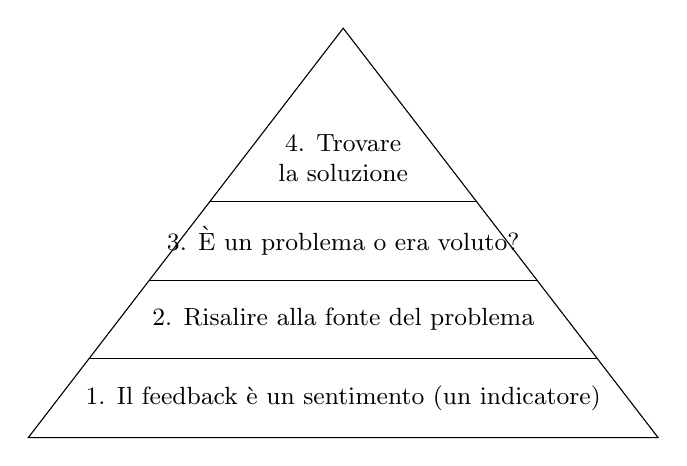
\begin{tikzpicture}[font=\small]
  \draw (0,0) -- (8,0) -- (4,5.2) -- cycle;
  \draw (0.77,1) -- (7.23,1);
  \draw (1.54,2) -- (6.46,2);
  \draw (2.31,3) -- (5.69,3);
  \node at (4,0.5) {1. Il feedback è un sentimento (un indicatore)};
  \node at (4,1.5) {2. Risalire alla fonte del problema};
  \node at (4,2.5) {3. È un problema o era voluto?};
  \node[align=center] at (4,3.55) {4. Trovare\\ la soluzione};
\end{tikzpicture}
\caption{La piramide del feedback come la descrive il relatore: si parte
dalla sensazione riferita da chi dà il feedback e si sale fino alla
soluzione. Ricostruzione schematica; la slide originale non è
disponibile.}
\label{p0:fig:piramide}
\end{figure}

\subsection{I feedback duri}

La piramide è anche un ottimo modo per \textbf{ricevere feedback in modo
professionale}, anche quelli difficili. Il relatore dà spesso feedback
\textbf{duri} ``anche per testarvi'': ``non perché sono stronzo''. Può dire
che una task è ``decente'', e dire anche tutto ciò che è sbagliato;
bisogna ricordarsi di lavorarci sopra e di \textbf{non prenderla sul
personale}. Magari sta testando la reazione, ``perché di fronte al vostro
capo in un'azienda non potete mandarlo a fanculo''.

% ---------------------------------------------------------------------
\section{La tecnica dell'iceberg}
\label{p0:sec:iceberg}

E se il problema è insormontabile? ``Allora, se il problema è
insormontabile, non esiste'', perché il relatore ha imparato la
\textbf{tecnica dell'iceberg} e la racconta ``come mi è stata spiegata''.
Non ha una base scientifica, avverte, ma a livello psicologico lo ha
aiutato molto. È una tecnica di \textbf{categorizzazione dei problemi}: non
è detto che un problema si risolva ``così'', ma la prima cosa da fare quando
lo si affronta è \textbf{descriverlo}, scriverlo in un testo, farne uno
schemino, e cercare di \textbf{classificarlo} in uno di quattro iceberg
(tabella~\ref{p0:tab:iceberg}). Se ne possono anche inventare di nuovi, per
esempio un iceberg ``basso e lungo'', che si estende per molto spazio invece
di essere largo.

\begin{table}[htbp]
\centering
\small
\begin{tabular}{@{}lp{4.4cm}p{5.4cm}@{}}
\toprule
\textbf{Iceberg} & \textbf{Che problema è} & \textbf{Come si affronta} \\
\midrule
\textbf{Alto} & Molto alto, insormontabile se lo si vuole scavalcare. &
Non lo si può prendere di petto: va \textbf{aggirato} in qualche modo. \\
\textbf{Largo} & Semplicemente molto grande, ma poco difficile. & Ci si
mette lì e \textbf{si fa fatica}. \\
\textbf{Nascosto} & Contiene situazioni problematiche, problemi nascosti. &
Obbliga a trovare il \textbf{problema reale} e a risolvere prima quello. \\
\textbf{Mostruoso} & Grande, difficile, complesso. & Richiede un
\textbf{approccio sistematico}, di solito suddividendolo in più parti. \\
\bottomrule
\end{tabular}
\caption{I quattro iceberg della tecnica dell'iceberg, come li presenta il
relatore.}
\label{p0:tab:iceberg}
\end{table}

Perché descrivere un problema con una forma ``geografica'' aiuta? Perché, se
lo si è descritto correttamente, si trova il modo di risolverlo. E, aggiunge
il relatore, la maggior parte delle volte si noterà che
\textbf{suddividere un problema in più parti} è la scelta migliore:
``splittate il problema in più parti, razionalizzate il problema''. Ed è
questo, conclude, il modo per affrontare al meglio il primo anno di AIV, o
tutti e tre.

% ---------------------------------------------------------------------
\section{Le domande finali}
\label{p0:sec:domande}

``Domande? Così recupero.'' E poi, davanti al silenzio: ``Oh, che
cavalcata! No, dai, vi prego, ditemi che avete dei dubbi''.

\subsection{A che cosa serve lo zone out?}

Una studentessa non ha capito il vantaggio dello zone out. Il relatore lo
spiega con la slide di figura~\ref{p0:fig:modi}: lo zone out
\textbf{potenzia la modalità diffusa}, e quindi la possibilità di trovare
soluzioni \emph{out of the box} che non si trovavano perché ci si
focalizzava troppo su un singolo punto. Se la soluzione è ``qui'' e ci si sta
concentrando ``qua'', non ci si arriva; in modalità diffusa il cervello vaga
e a un certo punto impatta nella soluzione. Inoltre rilassa la mente e, così
facendo, attiva il consolidamento, trasformando la working memory in
long-term memory. (Un partecipante commenta che sembra il cervello di un
personaggio di un film d'animazione\footnote{La trascrizione dice ``sembra
il cervello di Infeldo Sghetto 3'': il riferimento non è ricostruibile,
forse \emph{Inside Out}.}; ``vabbè, sì, certo, da qualche parte dovrà pure
venire fuori''.)

\subsection{La soluzione arriva sotto la doccia: e poi?}

Gabriele chiede: se finisco la giornata di lavoro con un problema aperto e
la soluzione mi viene a casa, sotto la doccia, mi rimetto a lavorare o me la
tengo per il giorno dopo? Nessuna delle due: \textbf{ci si prendono degli
appunti}. La tecnica migliore è avere sempre con sé un taccuino o il
cellulare (``non si dovrebbe fare, meglio un taccuino''). Il relatore tiene
il cellulare sul comodino: a volte, di notte, tornando dal bagno, gli viene
in mente qualcosa e se lo segna; a volte, fuori con il cane, si registra
mentre parla, e a volte si sblocca proprio parlando.

Tutto ciò che si è visto oggi, aggiunge, verrà ripreso durante il primo
anno, ma sono concetti che ``precedono il corso stesso'': durante l'anno non
c'è tempo, si fa il proprio corso. Qualcosa di neurocognitività tornerà a
narrative design e, al secondo anno, a game design, perché aiuta moltissimo
a \textbf{mappare il cervello del giocatore}, a capire come stimolarne certe
reazioni. Sarebbe bello approfondire, ma ``un po' rimane anche a voi'':
prendere le slide, approfondirle, leggerle.

\subsection{Arrivare da un'altra accademia}

Gabriele comincia direttamente dal secondo anno, avendo già fatto un anno in
un'altra accademia (``che purtroppo poi si sa com'è andata''); teme di
trovarsi spaesato non tanto per gli argomenti quanto per il metodo. Il
relatore distingue: \textbf{il metodo di studio è dello studente}; è il
\textbf{metodo di insegnamento} a essere diverso, e lo è (``senza nulla
togliere ai colleghi''): c'è un motivo per cui AIV fa nove ore di lezione a
settimana e il resto lo lascia allo studente. I consigli:
\begin{itemize}
  \item affrontare l'anno con \textbf{mentalità aperta}, senza crearsi
        pregiudizi solo perché arrivano cose diverse da quelle a cui si è
        abituati (e vale per tutti);
  \item se qualcosa non torna con l'istruzione precedente, \textbf{fare
        domande}, anche provocatorie: il relatore adora quando uno studente
        gli dice ``prof, questa cosa del viaggio dell'eroe io non la
        condivido, parliamone'' (``non vedo l'ora, davvero''), ``perché si
        apprende meglio''; avrebbe un problema se, da non professionista, si
        rifiutasse di rispondere per paura di come rispondere;
  \item ricordare che non è il metodo di insegnamento a cambiare lo
        studente: è il suo metodo di studio, ed è l'argomento ciò che si
        impara davvero, non il modo (``poi il modo aiuta molto, me ne rendo
        conto'').
\end{itemize}
Il problema vero, prevede il relatore, non sarà il metodo, ma il fatto che i
compagni hanno già un anno alle spalle e hanno affrontato cose che Gabriele
non ha visto, e su cui dovrà aggiornarsi. Il consiglio ``spassionato'':
\textbf{fare amicizia, aprirsi agli altri}. Ci si può far male, ``fa parte
del gioco''; ma essere aperti non vuol dire ``dare la propria password a
tutti'' (``a volte gli studenti mi prendono troppo alla lettera''): vuol
dire \textbf{dialogare}, e dialogare ``batte qualsiasi cosa''. Creare una
buona sinergia con la classe, cercando compromessi se serve.

\subsection{Come accorgersi di stare imparando un metodo sbagliato?}

Federico chiede come ci si accorge di stare imparando un metodo sbagliato,
per evitare il ``polso del chitarrista''. In parte sono i docenti a dirlo,
con i feedback: certe cose lo studente non può capirle da solo. Altre invece
le si nota confrontandosi con i compagni: ``cavolo, ma a me questa cosa
viene difficile, perché?''; ``mi viene, ma la sento macchinosa,
arzigogolata''. È possibile, non certo, che si stia avviando un effetto
Einstellung: si sta forse aprendo la bottiglia con una forza esercitatissima,
quando ne servirebbe molta meno.

\subsection{E all'università?}

Filippo, che frequenta anche l'università, chiede se questi metodi si
applichino a contesti più teorici, con meno possibilità di cambiare medium.
Il relatore premette di parlare ``con le pinze''. Ha fatto l'università e
``se ne pente parzialmente'': secondo lui l'università italiana ha
``tantissime competenze e conoscenze, ma pessime metodologie di
preparazione''; è soprattutto un istituto di ricerca e di studio, tranne le
facoltà pragmatiche (suo fratello è ingegnere elettrotecnico, con dottorato,
e doveva letteralmente fare circuiti; medicina è molto pratica). Ci sono
università di game design in Italia, ma con limiti: il ministero impone
esami come storia del videogioco, ``che è molto utile, ovviamente''.

Lui lavora per lo più con clienti, e al cliente non interessa la teoria né la
storia del videogioco fine a se stessa. La storia è utile \textbf{quando la si
applica}. Esempio, ripreso da ``stamattina'': il fatto che \emph{Pac-Man}
rallenti impercettibilmente mangiando i pallini\footnote{Si veda il
capitolo sul narrative design (sezione~\ref{p3:sec:mindset}). Il dettaglio
storico è che Pac-Man si ferma per un fotogramma a ogni pallino mangiato,
risultando un po' più lento dei fantasmi nei corridoi pieni di pallini.}
serve se un giorno, al lavoro, bisogna far rallentare il personaggio, senza
che il giocatore se ne accorga, quando fa certi passi, per renderlo più
raggiungibile e dargli la sensazione di ``oddio, non ce la faccio!'', magari
in una scena molto tesa di un horror: si prende la soluzione di Pac-Man e la
si adegua al contesto.

È molto importante che esista la ricerca: AIV ha bisogno degli studiosi,
il relatore lavora spesso con consulenti esperti di antropologia o di
storia. Ma non crede che un neolaureato sia pronto per l'industria, perché
molte tecniche della game industry non si insegnano all'università e
viceversa. Cita, senza nominarlo, uno studioso americano diventato un
professore importantissimo, che pubblica saggi di game design: saggi che
mostrano non un'incapacità di comprendere i framework, ma una comprensione
``in una scatola chiusa'', perché non li ha mai visti all'opera in un gioco.
È la differenza fra imparare a riparare un motore e fare davvero il
meccanico, quando le cose non sono uno a uno e vanno adattate.

Filippo precisa che la sua fatica all'università è data proprio dal ciclo
``testo, esame'', senza pratica, discussione e comunicazione. Il relatore
ribadisce che in AIV, in game design, tutte le task sono pratiche: al primo
anno su prodotti pubblicati (l'analisi del \emph{core loop} di un gioco, per
dire). All'università ci sono limiti: l'ultima volta che ha collaborato con
un ateneo gli hanno detto che il ministero impone un tetto del 30\% alle
attività di laboratorio. A lui il ciclo ``studio, studio, esame'' non
piace, perché nella vita reale non funziona così: ``il mio esame è la
pubblicazione'', che arriva dopo tre, quattro, cinque anni. Le conoscenze
generali che dà l'università sono ``imprescindibili ed enormi'', ma si
possono anche recuperare. Fa l'esempio della dizione nel doppiaggio: le
regole si assorbono, e al direttore interessa che la battuta sia detta bene;
e a volte, soprattutto gli americani, chiedono uno slang, e ``prova a
chiedere in università di farti imparare lo slang newyorkese di un
rapper''\footnote{La trascrizione dice ``addizione'' per ``dizione''. Il
passaggio è confuso, ma il senso è che certe competenze professionali si
apprendono sul campo, da altri professionisti, più che in università.}: gli
attori americani si formano facendo esperienza, andando da altri attori.

Non vuole criticare l'università: collabora con università e la rispetta. Ma
non gli piacciono quelli che, finito un corso universitario, pensano di
uscire e andare dritti a fare videogiochi. ``Io l'ho sentito sulla mia
pelle'': uscito dall'università non trovava lavoro e non capiva perché;
dieci anni dopo l'ha capito: quelle cose non le sapeva, e ha dovuto
``abbassare la cresta, fare un lavoro di umiltà e dire: ho studiato
altro''.

\subsection{Anatomia, per chi l'ha già studiata}

Una studentessa ha visto che al primo anno c'è anatomia e, avendo già fatto
tre esami di anatomia, chiede come sarà strutturato il corso. Va chiesto al
direttore di 3D art, nell'incontro dedicato (capitolo~\ref{p6:cap:3d}): il
relatore sa poco di quel corso, se non che al primo anno ci sarà una
collaborazione con i narrative per il \emph{world building} di un
gioco\footnote{Nella trascrizione: ``per il war building del giocato'',
probabilmente ``del giocattolo'': il corso di narrative prevede un modulo
di world building per i giocattoli (si veda il capitolo~\ref{p3:cap:narrative}).};
``vi diremo tutto a tempo debito'', in primavera.

\subsection{Le fiere: chi paga?}

Ultima domanda: se uno degli eventi di settore richiesti per il certificato
di eccellenza (sezione~\ref{p1:sec:eccellenza}) fosse una fiera come la
Gamescom, le spese sarebbero individuali? AIV fornisce \textbf{il biglietto
e l'alloggio} (dopo un'incertezza: ``vitto e alloggio\ldots\ scusatemi,
biglietto. No, alloggio'') ma non il trasporto, per \textbf{una fiera
all'anno}, a chi ha acquistato l'opzione \emph{Experience}; ``c'è scritto
sul sito''. La fiera la decide AIV ogni anno, sulla base di quella più
indicata; al terzo anno è al cento per cento la \textbf{First
Playable}\footnote{La trascrizione dice ``force playable''. La First
Playable è l'evento business dell'industria videoludica italiana che si
tiene a Firenze.}, ``perché alla First Playable bisogna andare''. A volte
le fiere mandano sconti, e la segreteria li comunica su Discord:
``sfruttateli assolutamente''. Ma AIV non ha la forza economica di mandare
tutti in fiera, solo chi ha l'Experience. Il relatore, che è di Milano, alla
Milan Games Week di solito scrive un messaggio per organizzare un
\emph{meet up}. La Gamescom è ``estremamente costosa'' anche da soli: chi
vuole andarci con AIV deve avere l'Experience, altrimenti si paga biglietto
e albergo. E la fiera, ogni anno, cambia.

%    % =====================================================================
%  Professioni 1 — I Dev Days: il metodo di AIV e i Dev Projects
%  Fonte: trascrizione dell'incontro di apertura dei Dev Days (AIV1):
%  un incontro online su Zoom di un'ora, il lunedì mattina della prima
%  settimana del primo anno, tenuto da Daniele Fusetto (direttore del
%  corso di narrative design e brand advisor dell'Accademia Italiana
%  Videogiochi) con Andrea Morini (direttore della didattica). Circa 31
%  partecipanti collegati su un centinaio di iscritti al primo anno;
%  slide condivise, un video di gioco senza audio, domande in chat.
%  Pacchetti richiesti nel preambolo del libro:
%    \usepackage[utf8]{inputenc}, \usepackage{booktabs},
%    \usepackage{tikz} con
%    \usetikzlibrary{arrows.meta,positioning,calc,fit}
%
%  Collocazione nel libro: parte "Alcune Professioni nel Mondo
%  Videoludico", dopo AIV0_mindset_e_best_practice (3.2).
%  Tutte le etichette di questo capitolo hanno il prefisso "p1:".
%  Il capitolo AIV0 (prefisso "p0:") rimanda a questo; questo rimanda ai
%  capitoli delle singole professioni (AIV2-AIV6).
%  La figura è una ricostruzione schematica di quanto il relatore spiega
%  con le slide, non una copia delle slide.
% =====================================================================

\chapter[I Dev Days e il metodo di AIV]{I Dev Days: il metodo di AIV,
la collaborazione fra discipline e i Dev Projects}
\label{p1:cap:devdays}

Ogni anno accademico, all'Accademia Italiana Videogiochi (\textbf{AIV}),
comincia con una settimana di incontri chiamati \textbf{Dev Days}. Lo scopo
è duplice: \textbf{impostare il lavoro} dell'inizio dell'anno e
\textbf{presentare a tutti gli studenti del primo anno che cosa faranno i
colleghi degli altri corsi}, perché, come si sentirà ripetere molte volte,
``la gaming industry è fortemente collaborativa'': i giochi si fanno in team,
e per lavorare bene con un game designer, un narrative designer, un
animatore, un programmatore o un 3D artist bisogna sapere che cosa fanno.
Questo capitolo raccoglie l'\textbf{incontro di apertura}; i capitoli
successivi raccolgono le presentazioni dei singoli corsi, cioè delle singole
professioni: game e level design (capitolo~\ref{p2:cap:gamedesign}),
narrative design (capitolo~\ref{p3:cap:narrative}), character animation
(capitolo~\ref{p4:cap:animation}), programmazione
(capitolo~\ref{p5:cap:programming}) e 3D art (capitolo~\ref{p6:cap:3d}).

A condurre l'incontro è \textbf{Daniele Fusetto}, direttore del corso di
narrative design e \emph{brand advisor} di AIV, che insegna in AIV dal 2019 e
in generale dal 2016; con lui c'è \textbf{Andrea Morini}, \textbf{direttore
della didattica}, che interviene a più riprese. L'incontro si tiene online,
su Zoom, il lunedì mattina, e dura \textbf{un'ora} (``abbiamo un'ora di tempo,
purtroppo''): non si aspetta molto chi è in ritardo, anche perché la
registrazione verrà caricata sulla piattaforma dell'accademia
(\emph{l'hub}). L'incontro non è facoltativo: ``i Dev Days non sono degli
incontri facoltativi'', bisogna almeno vederli in registrazione, ``altrimenti
si rischia di rimanere indietro fin dall'inizio''. Negli anni in cui
Fusetto e Morini hanno insegnato, ``sottovalutare una cosa del genere è di
solito il primo sintomo che qualcosa non va''.

Due avvertenze di lettura. La prima: la trascrizione è automatica e storpia
quasi sempre il nome dell'accademia (``Hive'', ``IVE'', ``Ive'', ``AIB'',
``AB'', ``IV'') e diversi titoli e termini; il capitolo usa sempre
``AIV'' e segnala in nota le ricostruzioni incerte. La seconda: molte
affermazioni riguardano l'organizzazione di AIV (calendari, regole,
certificati, opzioni di iscrizione) e valgono per l'anno a cui l'incontro si
riferisce; sono riportate come le dicono i relatori.

La data, dedotta, è \textbf{lunedì 5 ottobre 2026}\footnote{La data non è
detta. Si ricava da tre indizi: le lezioni dei corsi cominciano
``ufficialmente'' il 19 ottobre, quelle di narrative ``questo venerdì''; nel
capitolo sul narrative design, il giorno dopo, il relatore fissa la prima
lezione di narrative a ``venerdì 9 ottobre''; e nel 2026 il 9 ottobre è
venerdì. È una deduzione.}.

Il percorso del capitolo:
\begin{enumerate}
  \item l'avvio e la politica della webcam (sezione~\ref{p1:sec:avvio});
  \item che cosa sono i Dev Days e il calendario della settimana
        (sezione~\ref{p1:sec:devdays});
  \item il \textbf{metodo di AIV}: che cosa non si tollera e quattro cose da
        fare (sezione~\ref{p1:sec:metodo});
  \item \textbf{best practice} e \textbf{trappole}
        (sezioni~\ref{p1:sec:best} e~\ref{p1:sec:trappole});
  \item gli \textbf{obiettivi} dei corsi: portfolio, lavoro di gruppo,
        competenze trasversali (sezione~\ref{p1:sec:obiettivi});
  \item l'attestato di partecipazione e il \textbf{certificato di
        eccellenza} (sezione~\ref{p1:sec:eccellenza});
  \item i \textbf{Dev Projects} del secondo anno e la pipeline di sviluppo,
        con il caso di \emph{Beat of Rebellion}
        (sezioni~\ref{p1:sec:devprojects}--\ref{p1:sec:beat});
  \item perché parlarne il primo giorno, i falsi miti e le domande finali
        (sezioni~\ref{p1:sec:perche}--\ref{p1:sec:domande}).
\end{enumerate}

% ---------------------------------------------------------------------
\section{L'avvio}
\label{p1:sec:avvio}

Si comincia con qualche minuto di attesa: alcune persone sono in ritardo
``per problemi di hub'' o perché non hanno ancora fatto l'accesso. Il
relatore disabilita la sala d'attesa di Zoom e raccomanda di tenere
d'occhio il \textbf{Discord di AIV} e la propria \textbf{mail}. Poi
condivide le slide e comincia con la parte ``molto introduttiva'', mentre
arrivano gli ultimi.

\subsection{La webcam}

``Possibilmente accendete la webcam'': il relatore vuole vedere facce sveglie
``e anche le vostre camerette''. ``Mamma mia, è lunedì mattina per tutti'':
non c'è una regola che imponga di presentarsi a lezione ``belli e col volto
riposato'', ma la regola è che \textbf{ci si fa vedere}, anche quando si
segue da remoto. Non solo per buona educazione: i docenti devono vedere le
facce, le reazioni, e vogliono conoscere gli studenti anche fisicamente. Già
al tempo del COVID, ricorda, riconoscere dal vivo le persone viste online o
con la mascherina era stato ``un dramma''.

% ---------------------------------------------------------------------
\section{Che cosa sono i Dev Days}
\label{p1:sec:devdays}

L'agenda della mattina: che cosa sono i Dev Days, qual è il \textbf{metodo di
AIV}, e i \textbf{Dev Projects}, ``una cosa che voi vedrete al secondo
anno'', ma di cui i relatori vogliono dare un assaggio fin da oggi ``per
farvi capire che qua non si scherza''\footnote{La trascrizione dice
``farvi la capatanza'' e poi ``capatanta'': il senso è ``farvi fare una
capatina'', dare un assaggio. Il nome dei progetti del secondo anno
oscilla nella trascrizione fra ``Game Dev'', ``Dev Project'' e ``The
Projects''; il capitolo usa ``Dev Projects'' per i progetti e ``Game Dev''
per il percorso del secondo anno in cui si svolgono.}.

\subsection{Un'industria che lavora in team}

I Dev Days sono incontri dedicati, all'inizio del primo anno, a presentare
ciò che faranno gli altri colleghi e a impostare il lavoro. Il motivo è che
l'industria è fortemente collaborativa: \textbf{si sviluppano giochi in
team}, ``dalle 20 persone alle 400 persone''. Ci sono anche team più
piccoli, ma spesso un team di tre, quattro, cinque persone lavora molto con
\textbf{freelancer}. Esempio: si dice che \emph{Clair Obscur: Expedition 33}
sia stato fatto da trenta persone; ``non è vero, se vedete i credit, sono
400''\footnote{La cifra di 400 è del relatore. Il nucleo dello studio
Sandfall Interactive era di circa trenta persone; i titoli di coda includono
però numerosi collaboratori esterni (musica, doppiaggio, animazione,
outsourcing, localizzazione), che è appunto il punto del relatore.}. Fare
un gioco richiede un lavoro di team.

Al primo anno ognuno fa la propria disciplina: chi fa programmazione fa
programmazione, chi fa 3D fa 3D, e così per game design, character
animation, narrative design. Poi, all'inizio del secondo anno, ci si
incontrerà con tutti gli altri ``per fare insieme un videogioco''. Ma fin da
oggi bisogna capire che cosa faranno i colleghi e quali sono le altre
professioni insegnate in AIV, ``per meglio collaborare con gli altri''.

\subsection{Il calendario della settimana}

Per questo la settimana prevede \textbf{cinque incontri}, uno per ciascun
corso di AIV. Vanno seguiti \textbf{tutti}, e non sono solo per gli studenti
del corso presentato: ``sono per tutti gli studenti''. La presentazione di
game design spiega che cosa faranno i game designer durante l'anno, e la
devono seguire tutti, così che l'anno dopo, collaborando con loro, si sappia
più o meno che cosa fanno di solito. Lo stesso per narrative design,
character animation, programmazione e 3D art. L'obiettivo non è spiegare agli
studenti di quel corso che cos'è il corso (lo vedranno durante l'anno), ma
spiegare \textbf{a tutti} che cosa fanno le altre discipline. Tanto che
``probabilmente è meglio se, per esempio, la presentazione del corso di
programming la seguono più attentamente quelli che non faranno
programming''.

In più:
\begin{itemize}
  \item un incontro aggiunto quest'anno, il \textbf{giovedì mattina}, di
        un'ora e mezza, con Fusetto, anch'esso obbligatorio, sulla
        \textbf{comprensione del testo} (capitolo~\ref{pt:cap:comprensione}): ``mi spiace dirlo, ma negli ultimi
        anni ci siamo accorti che è difficile arrivare all'inizio di AIV con
        delle capacità di comprensione del testo ottime''. Non si parla di
        italiano di base né di una disciplina, ma di \textbf{comprendere
        ciò che le persone dicono e vogliono}, rispondere correttamente alle
        richieste dei docenti, evitare incomprensioni; si vedranno anche
        trucchi per comprendere meglio e per segnarsi le cose in modo da
        \textbf{saper porre domande}, ``perché è importantissimo porre
        domande'';
  \item un incontro il \textbf{martedì pomeriggio alle 14:30}, solo per chi
        si è iscritto entro il 31 luglio con la \textbf{Gamer Promo} o la
        \textbf{Dev Promo}: un incontro di \emph{mindset} e \emph{best
        practice} sulle pratiche migliori per imparare e apprendere
        durante l'anno (è il capitolo~\ref{p0:cap:mindset});
  \item per gli stessi studenti, la possibilità di una
        \textbf{mentorship} di un'ora con un tutor o un docente, ``per
        partire al meglio''. ``Sfruttatele, queste ore, perché l'anno scorso
        nessuno l'ha usata e poi dopo saltano fuori i problemi.'' Chi non
        ricorda se ha la promo può chiedere in segreteria.
\end{itemize}

% ---------------------------------------------------------------------
\section{Il metodo di AIV}
\label{p1:sec:metodo}

\subsection{In AIV si boccia}

``In AIV si boccia.'' Non è un'accademia ``dove vieni, paghi e passi
l'anno'': ci sono dei criteri. Il criterio principale è \textbf{non
consegnare le attività}, le cosiddette \textbf{task}, richieste durante
l'anno, perché la valutazione si fa su quelle: se non vengono consegnate, i
docenti non possono valutare.

Ma contano anche le \textbf{soft skill}, ``e se avete frequentato il nostro
open day lo sapete'': per passare l'anno bisogna
\begin{itemize}
  \item \textbf{interagire}: non isolarsi; chi è un po' introverso cerchi di
        uscire, di chiedere, di porre domande;
  \item \textbf{rispettare gli altri};
  \item essere \textbf{proattivi}: se viene in mente oggi che si deve o si
        può fare una cosa, non la si rimanda a domani; se si ha una domanda
        per la prossima lezione e si sa che il docente è raggiungibile per
        mail o per messaggio, non si aspetta la lezione.
\end{itemize}

\subsection{Tolleranza zero: bullismo, pregiudizi, cheating}

Su tre cose non c'è tolleranza.
\begin{description}
  \item[Bullismo.] ``Self-explanatory'', in tutte le sue forme: qualunque
        prevaricazione, anche implicita, ``non esiste''. Massima
        collaborazione e massima gentilezza, sempre.
  \item[Pregiudizi.] Si è in tanti e molto diversi, ognuno con le sue
        opinioni; ``a meno che voi non abbiate problematiche di tipo,
        diciamo, criminale, ma non credo'', bisogna partire dal presupposto
        che la persona che si ha davanti ha una sua storia, mettersi nei
        panni degli altri e \textbf{sospendere il giudizio}.
  \item[Cheating.] Fino a qualche anno fa voleva dire copiare dai compagni,
        avvantaggiarsi, manipolare la classe o i compagni per ottenere
        vantaggi non legati alla performance (``non faccio bene le attività,
        ma sono bravo a manipolare l'ambiente in modo da passare''). Negli
        ultimi due anni si è aggiunto \textbf{l'uso dell'IA}: è cheating
        quando, in un corso, viene detto di non usarla in un certo modo e la
        si usa così. Ogni corso ha il suo approccio (programmazione diverso
        da narrative, da game design, da character animation) e verrà detto
        che cosa si può fare e che cosa no. In narrative design, per
        esempio, è \textbf{severamente vietato scrivere con l'IA} per tutti
        e tre gli anni, ``vietatissimo'', fino a una lezione in cui il
        relatore spiegherà ``qual è l'unico modo, a mio parere'' per farsi
        aiutare dall'IA nell'atto della scrittura.
\end{description}

Ma cheating è anche copiare dai compagni: ``è successo, ce ne accorgiamo''.
I docenti vedono i compiti, notano forme usate nelle attività o
``spennellature, scolpiture nel modello 3D'' troppo simili. ``D'altronde, se
molti critici hanno capito che Palworld aveva copiato da Pokémon anche i
modelli 3D, si può fare''\footnote{È l'opinione del relatore, riportata
com'è. Le somiglianze fra i modelli di \emph{Palworld} e quelli dei Pokémon
sono state sostenute da utenti e commentatori dopo l'uscita del gioco
(2024), ma non sono mai state accertate; la causa intentata da Nintendo e
The Pokémon Company contro lo sviluppatore riguarda la violazione di
brevetti, non la copia dei modelli.}. Nel cheating c'è sempre una vittima,
la persona sfruttata o manipolata; ma soprattutto chi bara \textbf{fa un
danno a se stesso}: ``state pagando per imparare. Imparare voi.'' Chi usa
scorciatoie per passare l'anno e poi si ritrova senza conoscenze ha perso
un'occasione.

\subsection{Inquiry-based learning}

Poi ``quattro cose che dovete fare''. La prima: tutti i corsi di AIV sono
\textbf{inquiry-based}. ``Non esistono domande stupide, soprattutto il primo
anno.'' Molti studenti scrivono ``ho una domanda stupida'': no, non ce ne
sono. Arriva proprio in quel momento una domanda in chat (``scusi, ma i
corsi che ha fatto vedere prima sono online?''), e il relatore la usa come
esempio: ``anche qua, ragazzi, è importantissimo, \textbf{specificate bene
nelle domande}''. Si intende la \emph{lezione}, cioè il singolo incontro, o
il \emph{corso}, cioè tutto il corso? Gli incontri di questa settimana sono
tutti da remoto. Sara ha fatto una domanda ``per niente stupida'', perché
non era chiaro, ``e ha imparato anche qualcosa''\footnote{Nel capitolo sul
narrative design (sezione~\ref{p3:sec:skill}) il relatore torna su questo
episodio per spiegare perché tiene tanto alla precisione dei termini.}.
``Meno domande fate, meno imparate.''

\subsection{Un ambiente simulativo del mondo del lavoro}

La seconda: AIV è un \textbf{ambiente simulativo del mondo del lavoro}.
Tranne game programming, che ha test ed ``esamini'' (e i docenti di quel corso
spiegheranno perché), \textbf{non ci sono sessioni d'esame}, ma valutazioni
verbali tramite \textbf{task}. Durante molte lezioni, non tutte, il docente
dirà: ``voglio che mi consegniate questa task entro questa data''. Se la si
manca, la task è mancata e conta per il non passaggio dell'anno. Le task non
hanno tutte la stessa durata: in alcuni corsi sono molto corpose e
richiedono mesi; in game design e narrative sono più equilibrate, con task
da una o due settimane e altre da mesi. In sintesi: task settimanali,
mensili, trimestrali o annuali.

Bisogna entrare a poco a poco nell'ottica di un \textbf{approccio
professionale} al corso: ``prendetelo un po' come un lavoro''. Ogni giorno
si deve produrre, studiare, apprendere, confrontarsi, fare call, come in
qualsiasi lavoro, non solo nei videogiochi. La puntualità è importante;
tutti gli aspetti professionali ``in senso lato'' non sono semplicemente
graditi, ``sono mandatori''. ``Molto di più di quando i genitori ci dicevano,
alle superiori, devi pensare alla scuola come a un lavoro: questo è molto più
veritiero.'' E come nel lavoro si fanno meeting e incontri, ma si lavora
anche molto da soli: non bisogna sottovalutare il peso delle attività.

Le task sono \textbf{opportunità} per migliorarsi, ottenere più feedback e
\textbf{farsi notare dai docenti}, perché il 99\% dei docenti di AIV sono
lavoratori del settore: Fusetto stesso lavora nell'industria, sta facendo dei
giochi in questo periodo, e alcuni suoi studenti lavorano con lui. ``Non è un
modo per essere assunti'', ma permette di farsi notare per le proprie
capacità.

\subsection{Fail to learn}

La terza: \textbf{fallire}. Una delle cose più importanti da fare al primo
anno è fallire e imparare: non \emph{fail for}, ma \emph{fail to
learn}\footnote{Così nella trascrizione; il senso è ``fallire per
imparare''.}. Se si sbaglia, si ricevono feedback e si trovano soluzioni, e
piano piano si impara a trovare soluzioni ai propri fallimenti; si noterà
``un aumento notevole'' delle proprie capacità. Il consiglio pratico:
prendere una task di settembre, metterla ``in una giara virtuale'' (un
drive), lasciarla lì e a gennaio confrontarla con una task di gennaio. Se le
differenze non si notano, è perché non si è fallito e non si è imparato: ``è
una campanella d'allarme''.

\subsection{Mettere in pratica, ogni giorno}

La quarta: i corsi di AIV richiedono di \textbf{mettere in pratica} ciò che
si apprende. Perché solo \textbf{nove ore di lezione a settimana}, e non
lezioni tutte le mattine come in altre accademie? Perché bisogna avere il
tempo di mettere in pratica teoria e pratica viste a lezione: ``se io non vi
do almeno 20 ore alla settimana per mettere in pratica quello che vi insegno,
è difficile''. Il relatore porta il proprio esempio\footnote{Poco prima il relatore dice ``come diceva Andrea'': nella trascrizione i cambi di voce fra i due relatori non sono segnati, e l'attribuzione di alcuni passaggi è incerta. Qui, dal contesto (``io so programmare un pochettino'', ripetuto anche nel capitolo~\ref{p3:cap:narrative}), parla con ogni probabilità Fusetto.}: pur considerandosi un artista usa spesso Unreal Engine, e nel lavoro si acquisiscono capacità trasversali; sa
programmare ``un pochettino'', ma non ci riuscirebbe se non si mettesse
tutti i giorni quindici minuti a programmare\footnote{La trascrizione dice
``io non saprei programmare se io tutti i giorni mi mettessi lì 15 minuti a
programmare'': manca evidentemente un ``non''.}. Bisogna impegnarsi ogni
giorno nella propria disciplina. Altrimenti ci si sveglia all'ultimo, si
imparano le cose al momento del bisogno (magari anche bene), ma nasce una
sensazione di \emph{burnout}, ``e poi il burnout lo prendete''.

Quindi: mettersi da parte del tempo ogni settimana per applicare ciò che si
vede a lezione, farsi domande, fare domande ai docenti, e
\textbf{impegnarsi al massimo sulle task}. Con alcune regole:
\begin{itemize}
  \item se una task sembra \textbf{semplice}, la si fa \textbf{due volte}:
        forse si sta sopravvalutando se stessi. Se è davvero semplice, si
        chiede al docente se c'è la possibilità di avere qualcosa in più
        (``a me sembrava semplice, secondo te l'ho fatta bene?''), e magari
        arriva qualcosa di extra;
  \item se sembra \textbf{troppo difficile}, la si tenta comunque, perché
        una delle basi dell'apprendimento è l'\textbf{alternanza di
        difficoltà}: alternare task semplici e difficili fa apprendere
        meglio che fare solo le une o solo le altre;
  \item se la si finisce \textbf{in anticipo}, la si approfondisce e la si
        rifà. ``È noioso? Sì. È lungo? Sì. È pesante? Sì. Però è il
        migliore.''
\end{itemize}

\subsection{Consegnare in anticipo per avere un feedback?}

Una domanda in chat: si può consegnare una task in anticipo per ricevere un
feedback e correggere gli errori? Sì, risponde il relatore, ma con due
precisazioni. Di solito i docenti danno tutti i feedback contemporaneamente,
``perché ho bisogno di vedere anche il confronto con la classe''; si può
però mandare una task e fare \textbf{domande specifiche}. E bisogna
aspettarsi che i docenti non rispondano direttamente: a lui capita spesso
che gli chiedano ``Daniele, secondo te questa cosa l'ho spiegata troppo?
l'ho fatta troppo così?'', e lui risponde ``secondo te l'hai fatta
troppo?''. ``Non frustratevi per questo'': deve insegnare in qualche modo ad
andare avanti da soli. Non è detto quindi che si ottenga una risposta, ma si
avranno indicazioni, e chi consegna uno o due giorni prima può ricevere
feedback aggiuntivi. Una condizione: se si consegna in anticipo, deve
essere perché si è dato il massimo, non perché si è ``tirato via'' per
consegnare prima. E non è banale: nella sua carriera, ``ma anche
attualmente'', quasi nessuno riesce a consegnare in anticipo.

% ---------------------------------------------------------------------
\section{Best practice}
\label{p1:sec:best}

Le \textbf{best practice}, ``soprattutto per chi segue in remoto''.

\paragraph{Camera sempre accesa.} Vale per chi segue da remoto, ma anche per
chi segue in presenza e capita di seguire una lezione online. E capiterà:
``in Italia abbiamo una maledizione, si chiamano scioperi''. Spesso il
venerdì ci sono scioperi di mezzi, treni, autostrade, a Roma e a Milano
(``l'anno scorso Milano è stato un delirio''); per non perdere la lezione,
se c'è sciopero e il docente non può venire in presenza, la lezione del
venerdì si trasforma in lezione da remoto. In quei casi la camera va tenuta
accesa: al docente serve per vedere i volti (``vedo il volto di Mattia, di
Gabriele, di Emanuele, di Davide, vedo come sono messi, se stanno capendo
oppure no''), e allo studente è ``una scusa in meno per distrarvi'', perché
``la distrazione è sempre dietro l'angolo''.

\paragraph{Prendere appunti.} Cartacei o digitali, non importa. Non bisogna
fare come i camerieri, che pensano di prendere gli ordini a mente e
puntualmente se li dimenticano; il fenomeno ha anche un nome, l'\textbf{effetto
Zeigarnik}, ``se volete potete andarlo a cercare''\footnote{La trascrizione
dice ``Zygarnik Effect''. L'effetto è ripreso e discusso nel
capitolo~\ref{p0:cap:mindset} (sezione~\ref{p0:sec:memoria}).}.

\paragraph{Interagire con i docenti.} Fare domande durante le lezioni.

\paragraph{Rivedere le registrazioni.} Soprattutto per gli
\textbf{studenti lavoratori}. Ogni settimana ci sono nove ore di lezione; chi
lavora e sa che ne perderà tre a settimana ha il compito ``tassativo'' di
recuperarle nel weekend. Altrimenti la settimana dopo diventano sei, poi
nove, ``e improvvisamente quelle tre ore diventano 18''. ``Io ho studenti che
arrivano a giugno e mi dicono: prof, devo ancora recuperare lezioni di
febbraio. E io non rido'', perché le lezioni sono spesso consequenziali. Il
sistema di registrazione dà pochi problemi: entro 24 ore circa le
registrazioni sono disponibili (``scongiurando bug e problematiche di
cloud''). ``Guardatevele, riguardatevele, mettete il 2x piuttosto.''

\subsection{Quanto restano le registrazioni, e a che cosa servono}

A una domanda in chat uno dei relatori risponde che le registrazioni restano
attive almeno fino all'inizio dell'anno successivo, verso fine settembre,
quando si cominciano a staccare le vecchie per fare spazio al nuovo anno.
Si possono quindi recuperare anche d'estate: chi, per motivi di lavoro, non
ha consegnato abbastanza e ha bisogno di tempo per recuperare, lo ottiene
durante l'estate, con l'accesso alle lezioni.

Le registrazioni, aggiunge Fusetto (richiamando un'osservazione di Morini), servono anche ad altro: ci
saranno cose che non riescono, problemi che non si risolvono, cose non
capite. È vero che i docenti sono facilmente raggiungibili su Discord, ma
quella è \textbf{l'ultima chance}: bisogna imparare a \textbf{risolvere i
problemi da soli}. Se è qualcosa trattato a lezione, si riguarda la
registrazione, si chiede ai colleghi, si guardano gli appunti e le
dispense; si chiede a Google (``non riesco a installare questa cosa''), si
chiede ``alla maledettissima intelligenza artificiale''. Solo se nulla di
tutto questo aiuta, perché il problema è particolarissimo, si va dal
docente. Bisogna sforzarsi di non avere ``la pappa pronta'': fa parte del
\emph{problem solving}. È come con un datore di lavoro: non si va dal capo a
ogni problema, prima si cerca di risolverlo. Al primo anno, precisa
Fusetto, va bene scrivere qualsiasi domanda quando si vuole (e così per gli
altri docenti, secondo le indicazioni che daranno); al secondo anno
comincerà a dire ``guarda che per questa cosa potevi anche non scrivermi'',
perché nel lavoro non si può scrivere al capo ``ogni due per tre''.

Chi ha bisogno di ancora più tempo ha l'opzione \textbf{Companion},
acquistabile anche durante l'anno accademico, che dà accesso alle lezioni
per un altro anno: è pensata per chi ha davvero bisogno di più tempo, e
richiede un processo dedicato (le lezioni vengono spostate su un altro
server), con più tempo, costo e lavoro. ``Non è un obbligo, ovviamente.''

% ---------------------------------------------------------------------
\section{Trappole}
\label{p1:sec:trappole}

Poi le \textbf{trappole}, ``trappoloni''.

\paragraph{``Mi basterà ascoltare?''} Molto spesso no.

\paragraph{``Posso fare altro nel mentre?''} ``Altro trappolone enorme, che
l'anno scorso ha fatto cadere tantissime persone'': ``tanto sono indicazioni
di massima, poi mi rivedo la lezione''. No. Andrea Morini, ``come direttore
didattico, terribile'', avverte che i docenti sanno se, durante una lezione
da remoto, qualcuno guarda una serie TV o gioca; e ci sono stati studenti
che giocavano in aula mentre il docente spiegava. ``Non è ammissibile in
nessun caso, mai'': a quel punto interviene lui, ``io sono quello cattivo''.
Massima attenzione: \textbf{nessuno è multitasking}, ``è falso''. Si segue la
lezione e basta, si spegne il cellulare. Anche perché seguire più cose
contemporaneamente \textbf{affatica}, anche se non sembra.

\paragraph{``Farò due minuti di ritardo, che sarà mai?''} C'è un ritardo
ammesso di 5--10 minuti, ma \textbf{non c'è il quarto d'ora accademico},
a meno che il docente non lo conceda. Se il docente dice ``10:10 in aula'' o
``14:10 in aula'', a seconda dell'orario, o ``questo orario, \emph{sharp}'',
bisogna essere puntuali.

\paragraph{``Sono come tutorial.''} ``Questo è un grande altro tema'': il
trappolone del ``tanto è come un tutorial di YouTube, poi me lo seguo in
registrazione''. No: rispetto a un corso su YouTube, su Udemy o a un corso di
formazione registrato, si ha un vantaggio, \textbf{si può chiedere
direttamente al docente}, che è un esperto del settore (``nel corso di Udemy,
vi posso assicurare, non sapete chi è il docente''). Anche quando una
lezione è un tutorial, ``non è davvero un tutorial'': si può chiedere di
rispiegare. E, ricordando le soft skill (niente pregiudizi, rispetto), se un
collega chiede ``prof, può rispiegare?'' e noi avevamo capito, anche se
pensiamo di annoiarci, conviene pensare ``magari mi sono perso comunque
qualcosa''. ``Non è un errore rispiegare, anzi, molto meglio rispiegare.''

% ---------------------------------------------------------------------
\section{Gli obiettivi dei corsi}
\label{p1:sec:obiettivi}

\subsection{Obiettivi primari: portfolio, problemi reali, lavoro di gruppo}

Il primo obiettivo, tutto l'anno e tutti gli anni, è \textbf{lavorare per
realizzare un portfolio}. Oltre al ``pezzo di carta'', la cosa principale per
entrare nella game industry è il portfolio: i giochi creati, i prodotti
fatti, i modelli 3D per i 3D artist, il software per i programmatori, gli
script per i narrative designer, le task per i game designer, le animazioni
per i character animator.

Attenzione, ``soprattutto programmatori e 3D artist, che di solito
sottovalutano questo punto'': \textbf{i giochi pubblicati sono l'elemento di
portfolio più importante di tutti}, più degli altri giochi fatti e ancora di
più delle task. Quando un selezionatore delle risorse umane, ``ma soprattutto
un lavoratore di un'azienda videoludica'', valuta un portfolio, considera più
importanti i giochi pubblicati su itch.io o su Steam, anche con gli amici
per una jam (non devono essere tripla A, devono essere accessibili), di
qualsiasi elemento legato a giochi mai pubblicati. ``Ho fatto un modello 3D.
È stato pubblicato in un gioco? No? Vale di meno'', e vale ancora meno della
task. Per questo, andando avanti negli anni, bisognerà riuscire sempre di più
a realizzare giochi, e giochi pubblicati; e qui AIV aiuta con i Dev Projects.

Il secondo obiettivo è lavorare su \textbf{problemi e progetti reali}: c'è
``un implicito accordo'' fra docenti e studenti per cui i docenti danno
problemi che davvero si troveranno nell'industria, quelli che si affrontano
tutti i giorni. E il terzo è lavorare \textbf{in gruppo} per potenziare le
soft skill. ``Fondamentale'': bisogna creare fin dai primi mesi un
\textbf{ottimo corpo classe}, una buona sinergia fra studenti. Secondo i
numeri e le analisi di AIV (``e Andrea ve lo può confermare''), le classi
molto unite, con studenti che si supportano, hanno molte più possibilità e
meno problemi di quelle che litigano. ``È banale da dire'', eppure non si sa
quante volte micro faide e micro litigi nati per niente creino problemi
``atroci, enormi''.

Andrea Morini aggiunge che queste cose derivano spesso da una sbagliata
considerazione del proprio \textbf{ego}: ``qui non c'è ego''. Non vuole
vedere nessuno che, per motivi di ego, rallenti o danneggi i colleghi,
anche involontariamente, senza accorgersene e senza malizia, ``ma succede''.
``Qui l'ego lo potete mettere da parte, e allora andiamo tutti d'accordo.''

\subsection{Obiettivi secondari: competenze a T rovesciata}

Fra gli obiettivi secondari ci sono le \textbf{competenze a T
rovesciata}\footnote{La trascrizione dice ``competenze ti è rovesciata'' e
``competenza tirovesciata''. Il riferimento è al modello delle competenze
``a T'' (\emph{T-shaped skills}): una competenza profonda in una
disciplina (l'asta verticale) unita a una conoscenza più ampia delle
discipline vicine (il tratto orizzontale). Il relatore lo chiama ``a T
rovesciata'', con il tratto orizzontale alla base.}. Nell'industria si torna
a parlare del fatto che stanno tornando lentamente i \textbf{generalisti}.
È un ciclo costante dagli anni Settanta, da quando sono nati l'informatica e
il software: le industrie tecnologiche preferiscono, alternativamente,
persone con competenze variegate che sanno lavorare su tutto un prodotto (i
cosiddetti \emph{full stack}: programmatore full stack, game designer full
stack) oppure persone molto specializzate, \textbf{verticali}. Fino a prima
dell'IA era molto importante essere ``terribilmente verticali''; proprio in
questi giorni Fusetto e Morini si sono confrontati sul fatto che molte
aziende cominciano a pensare di tornare indietro e avere generalisti,
perché con l'IA c'è ``questa sorta di verità e illusione'' (``lo sapremo
solo con calma nel tempo'') che una persona con competenze differenti
funzioni di più.

AIV insegna a T rovesciata, e questo mette gli studenti in una sorta di
``bunker protettivo'': i corsi sono verticali, ma dentro la propria
verticalità si vedono tante cose. In game design si è verticali sul game
design, ma si vede Unreal, si programma con i Blueprint, si fa level design,
combat design: ``vedete tutto quello che c'è nel game design''. E nessuno,
nell'industria, chiederà a un game designer di fare modelli 3D: magari
competenze di base per mettere gli asset nell'engine, ``ma non vi potrete
sostituire a un modellatore 3D''. Bisogna quindi essere
\textbf{intraprendenti}: imparare tutte le sfaccettature del proprio lavoro
e, al secondo e terzo anno, nei lavori di team, imparare anche \textbf{per
osmosi} da ciò che fanno i colleghi.

Andrea Morini aggiunge un dettaglio: AIV ``si mette sempre in discussione''.
Un paio di volte l'anno va a vedere ``non so quante'' \emph{job
description}, le posizioni aperte, per verificare quanto sia vero che il
generalista sta tornando di moda: ``poco, poco''. Oggi le posizioni aperte
sono ancora ``estremamente verticali, non se ne esce''; nei piccolissimi
studi di tre o quattro persone un generalista può essere più apprezzato,
altrimenti no. Quindi, all'uscita, ci si propone come \textbf{specialisti
della propria disciplina}, e in azienda scopriranno che si sa fare anche
altro. Spesso si entra con una qualifica e si esce con un'altra (magari si
entra in un ruolo junior di base, ``adesso poi dovremo vedere che cosa
succederà con le posizioni junior''), e nulla vieta di fare carriera
all'interno.

\subsection{Competenze spendibili fuori dal settore}

Le competenze sono importanti anche per l'\textbf{extrasettore}: in tutti i
corsi si imparano cose spendibili anche fuori dalla game industry, e questo
serve per due motivi. Se non si trova lavoro nell'industria, si possono usare
altrove; e se dopo tre anni ci si convince che quello non è il proprio
futuro, idem. Fusetto ha ``moltissimi studenti'' che hanno cambiato carriera
usando le competenze acquisite. Si augura che tutti facciano il lavoro per cui
si sono iscritti, ma ``non abbiamo la palla di cristallo'': meglio prevenire
che curare.

Al terzo anno, inoltre, si fanno molte lezioni, anche con i \textbf{Career
Days}, sulle \textbf{competenze imprenditoriali} e sul
\textbf{freelancing}: non c'è solo l'assunzione in azienda, c'è il freelance
(Fusetto è freelancer) e c'è chi vuole aprire un'azienda. L'Italia, dice,
ha due cose ``fenomenali'': la capacità degli italiani di essere imprenditori
e di sognare in grande, e ``la stragrande capacità del governo italiano di
mettere burocrazia per impedire l'imprenditorialità''. Sulla burocrazia non
si può lavorare, ma si può diventare intraprendenti, evitare errori enormi e
diventare imprenditori migliori, ``per esempio degli americani'': un
americano apre una società in due ore con una carta di credito e al primo
problema si blocca; un italiano dice ``che sarà mai, ho passato ore
chilometriche a fare burocrazia''.

% ---------------------------------------------------------------------
\section{Attestato di partecipazione e certificato di eccellenza}
\label{p1:sec:eccellenza}

La parte sui certificati la presenta Andrea Morini. Da qualche tempo AIV ha
introdotto l'\textbf{attestato di partecipazione}, che attesta che si è
partecipato al corso, cioè che si è fatto ciò che il corso richiede:
\textbf{consegnare le task}. Non basta essere stati presenti (``è implicito
che è importante''); è ancora più importante \textbf{produrre}, così da potersi
confrontare su ciò che si produce.

Accanto c'è il \textbf{certificato di eccellenza}\footnote{La trascrizione
dice ``il CTV Audi Eccellenza'' e ``il certificato di scelta'': si tratta in
entrambi i casi del certificato di eccellenza.}, per chi dà importanza a
tutto ciò che si sta dicendo e applica queste best practice. I requisiti
sono tre:
\begin{enumerate}
  \item \textbf{aver prodotto molto e bene}: essere promossi, aver
        consegnato \textbf{tutte} le task dell'anno (``per alcuni corsi sono
        tante'') e superato gli eventuali test; oppure aver consegnato
        \textbf{almeno l'80\%} delle task, ma con \textbf{metà di questo 80\%
        valutata eccellente}, a discrezione del docente;
  \item \textbf{aver partecipato ai Dev Projects}, collaborando fino al
        \textbf{completamento} del progetto (non necessariamente alla
        pubblicazione); se per qualsiasi motivo non è stato possibile
        (``non perché lavorate, non potete'', ma perché il progetto è stato
        chiuso perché non andava bene, ``mille motivi''), aver partecipato
        almeno a delle \textbf{game jam}: ``è il \emph{second best}'';
  \item aver partecipato \textbf{almeno a un secondo evento di settore}
        ogni anno, oltre alla jam: ``sembra che dobbiamo metterla come un
        premio, e invece dovrebbe essere la prassi''.
\end{enumerate}

Gli eventi di settore sono fondamentali soprattutto per il
\textbf{networking}: crearsi una rete di conoscenze nell'industria che, in
futuro, ``probabilmente mi agevolerà'' nel trovare lavoro. Va fatto da
subito, non alla fine del corso: le game jam sono un modo, gli eventi di
settore (AIV ne indicherà alcuni; sulla slide ce ne sono degli esempi) sono un
altro. ``Dovete farlo''; AIV lo riconosce con il certificato. ``Dovreste
farle a prescindere, però se le fate a noi piace, tra virgolette, premiarvi
con un bollino di eccellenza.''

Il certificato ha un valore anche nel curriculum. Come Morini ha spiegato
``anche ieri all'open day'', quando si selezionano persone per un lavoro si
fa una prima scrematura cercando almeno un certificato di scuola, università
o accademia equiparata (``non importa laurea o non laurea, all'estero''):
l'importante è aver fatto un percorso dopo le superiori. Poi si guarda il
portfolio, ma si guardano anche i \textbf{meriti}. Il certificato di
eccellenza è ``un'ottima occasione per brillare''.

% ---------------------------------------------------------------------
\section{I Dev Projects}
\label{p1:sec:devprojects}

``Cerchiamo di correre verso la fine, abbiamo ancora un quarto d'ora
circa.'' ``Voi siete qua perché volete fare giochi, giusto? Quindi
facciamoli.''

\subsection{Che cosa sono}

Come si fa un gioco? Di solito ci sono tre fasi, mutuate dal cinema:
\textbf{pre-produzione}, \textbf{produzione}, \textbf{post-produzione}. Da
questo metodo AIV prende il modello di sviluppo del secondo anno.
All'inizio del secondo anno, dopo i \emph{pressure test} e i test di inizio
anno, quindi intorno a novembre (quest'anno il \textbf{18 novembre}), gli
studenti del secondo anno vengono divisi in \textbf{gruppi
interdisciplinari}, che devono fare il \textbf{pitch} di un gioco da
sviluppare nei \textbf{due anni} successivi. I migliori vengono pubblicati.

Si chiamano \textbf{Dev Projects} e sono ``sviluppo ludico reale in contesto
didattico'': a AIV non piace chiamarli progetti studenteschi, ``perché non
lo sono''. Sono supervisionati da un comitato di esperti (``una
controlunca'' nella trascrizione), di cui fa parte anche Fusetto, dal
concept alla release. I migliori vengono pubblicati ``live'' su
\textbf{Steam} e su \textbf{Epic Games Store}: dall'anno scorso, dice il
relatore, AIV è diventata una delle tre accademie in Europa, e l'unica in
Italia, a poter pubblicare i giochi degli studenti su Epic\footnote{È
un'affermazione del relatore, non verificata.}.

``Pubblicati'' non vuol dire messi online per amici e parenti: sono
prodotti \textbf{gratuiti} che vengono scaricati \textbf{fra le 60.000 e le
100.000 volte}; \emph{Steam Rush} è stato giocato da 100.000 persone; le
recensioni medie vanno da ``positive'' a ``molto positive''. ``Non stiamo
parlando di piccoli giochi che fate nel giardino di casa'', ma di prodotti
che possono fare la differenza fra essere assunti o no: molti degli autori
di \emph{Steam Rush} sono stati assunti proprio perché l'avevano nel
portfolio.

\subsection{I giochi pubblicati}

Una slide mostra i giochi pubblicati finora (``da aggiornare'').
L'elenco, nella trascrizione, è in buona parte storpiato\footnote{La
trascrizione riporta: ``l'Eder, il Beautiful, il Duality Shift \ldots\ Tito
Rebello e Duality Shift sono già stati pubblicati. Powerful viene
pubblicato a breve. Solarpunk e D'Angelo Augusto avranno una storia un po'
più lunga. Operation Remote, Bolbuletti e Steamrash sono già fuori. Gunpire
e Ancora For Atlanti \ldots''. ``Tito Rebello'' è con ogni probabilità
\emph{Beat of Rebellion}, il gioco mostrato subito dopo; gli altri titoli
non sono ricostruibili con certezza e sono riportati come appaiono.}: fra i
titoli riconoscibili ci sono \emph{Beat of Rebellion}, \emph{Duality
Shift}, \emph{Operation Remote} e \emph{Steam Rush}, già usciti; un altro
uscirà a breve; due progetti ``avranno una storia un po' più lunga''. Due
giochi, \emph{Gunpire} e un altro, sono stati anche \textbf{finalisti al Game
Development World Championship 2025}.

\subsection{Perché sono importanti}

Perché parlarne già adesso, un anno prima? Perché i Dev Projects sono ``la
vostra chance principale per lavorare in questa industria''. ``Voi siete qua
per fare giochi, dimostratelo'': dimostrare di saper lavorare in team, di
superare problemi interpersonali, di capire come lavorano gli altri
dipartimenti, di costruire un portfolio, di lavorare in modo simulativo
del mondo del lavoro.

Alla fine del terzo anno, insieme al certificato di partecipazione, AIV
consegna \textbf{la custodia del gioco} con dentro la scheda SSD o la chiave
USB con la \emph{build} (``non c'è la slide, ma la dovrei mettere''): per far
capire di aver fatto una scuola che ha fatto realizzare un prodotto reale. I
giochi vengono poi pubblicati \textbf{nei 6--8 mesi successivi} al terzo
anno, durante i quali AIV continua a seguire gli studenti
\textbf{gratuitamente}: Fusetto e \textbf{Giacomo Caneschi}, direttore di 3D
art (capitolo~\ref{p6:cap:3d}), seguono i prodotti e lo sviluppo ``perché ci
piace che i nostri studenti pubblichino''.

% ---------------------------------------------------------------------
\section{La pipeline di sviluppo}
\label{p1:sec:pipeline}

Come avviene lo sviluppo? Saperlo serve già al primo anno, perché molti
faranno progetti nella propria classe. La pipeline mostrata è questa
(figura~\ref{p1:fig:pipeline}):
\begin{description}
  \item[Pre-produzione.] Un \textbf{concept}, un \textbf{vision document},
        una fase di \textbf{ricerca}.
  \item[Vertical slice.] ``Un prototipo prototipato''\footnote{Così nella
        trascrizione: il senso è un prototipo rappresentativo del gioco
        finito, completo in una sua piccola porzione.}.
  \item[Produzione.] Design, development, prototipo.
  \item[Release candidate.] Il candidato al rilascio. Un tempo, dice il
        relatore, nell'industria si chiamava \emph{Release to Market},
        perché era la build che si metteva nei CD; oggi che molti giochi
        sono pubblicati in digitale si chiamerebbe \emph{Release to
        Marketing}, la build consegnata al marketing per la
        promozione\footnote{La sigla in uso nell'industria del software è
        RTM, \emph{Release to Manufacturing}: la versione consegnata alla
        produzione fisica dei supporti. ``Release to Market'' e ``Release to
        Marketing'' sono le espansioni date dal relatore; la seconda, in
        particolare, sembra una sua interpretazione.}.
  \item[Polishing, marketing, community management.] Chi segue, come il
        relatore, \emph{Control Resonant} può vedere quanto marketing si
        sta facendo per spingere il gioco: ``tantissimo''.
  \item[Customer care.] Un gioco è un software, e serve assistenza al
        cliente: magari un cliente l'ha comprato ma non riesce a
        scaricarlo.
\end{description}
Un gioco, insomma, non finisce al rilascio: ci sono i DLC, ci sono le patch.
``Il \emph{Control} è già stato patchato tre volte, siamo alla 1.4, è uscito
da una settimana''\footnote{La trascrizione dice ``il controverso è già
stato patchato'': dal contesto è \emph{Control Resonant}, citato poco prima.
I dettagli sulle patch sono quelli riferiti dal relatore.}. ``C'è da
lavorare anche dopo.''

Una precisazione terminologica, valida per tutto l'anno: ``io parlo in
termini tecnici, se non è chiaro, chiedete''. Per \textbf{build} si intende
l'eseguibile del gioco, il file \texttt{.exe} che si può cliccare e lanciare
(per esempio da Steam); più in generale, la build è \textbf{la versione del
gioco su cui si sta lavorando}.

\begin{figure}[htbp]
\centering
\begin{tikzpicture}[
  fase/.style={draw, rounded corners, align=center, font=\footnotesize,
               minimum height=1.25cm, text width=2.05cm},
  >=Stealth, node distance=0.35cm]
  \node[fase] (pre) {\textbf{Pre-produzione}\\ concept, vision,\\ ricerca};
  \node[fase, right=of pre] (vs) {\textbf{Vertical\\ slice}};
  \node[fase, right=of vs] (prod) {\textbf{Produzione}\\ design, sviluppo,\\ prototipo};
  \node[fase, right=of prod] (rc) {\textbf{Release\\ candidate}};
  \node[fase, right=of rc] (post) {\textbf{Post-produzione}\\ polishing, marketing,\\ community, assistenza};
  \draw[->, thick] (pre) -- (vs);
  \draw[->, thick] (vs) -- (prod);
  \draw[->, thick] (prod) -- (rc);
  \draw[->, thick] (rc) -- (post);
  \draw[->, thick, dashed] (post.south) -- ++(0,-0.6) -| node[pos=0.25, below, font=\scriptsize]
       {patch, DLC: il lavoro continua dopo il rilascio} (prod.south);
\end{tikzpicture}
\caption{La pipeline di sviluppo dei Dev Projects come la presenta il
relatore. Ricostruzione schematica.}
\label{p1:fig:pipeline}
\end{figure}

% ---------------------------------------------------------------------
\section{Un caso: l'evoluzione di \emph{Beat of Rebellion}}
\label{p1:sec:beat}

Per far vedere come cambia un gioco lungo la pipeline, il relatore mostra
\emph{Beat of Rebellion}, uno dei giochi pubblicati l'anno precedente.
\begin{itemize}
  \item \textbf{Pre-produzione.} I bozzetti, il \emph{concept document} e
        una ``build ipotetica'', il prototipo realizzato nella fase di
        ricerca\footnote{La trascrizione dice ``la GIM che avevano nella fase
        di ricerca'': la parola non è ricostruibile; dal contesto si tratta
        della build prototipale di quella fase.}.
  \item \textbf{Vertical slice.} Dopo circa sei mesi, da gennaio a giugno,
        la vertical slice. La slide mostra il \emph{level design} visto
        dall'alto: ``non è così il gioco'', che è isometrico e segue il
        personaggio.
  \item \textbf{Produzione.} Il lavoro sul livello: il livello c'era già,
        ma è stato annotato, è stato sviluppato il personaggio e l'aspetto
        grafico. Si vede il livello crescere, e si nota la differenza a
        livello di \textbf{texturing}: un modello 3D senza texture, cioè
        senza quell'aspetto di superficie, e lo stesso modello con la
        texture. ``Queste parole imparatele tutti, non solo i grafici 3D.''
        È stato fatto anche \emph{character development} degli NPC.
  \item \textbf{Release candidate.} Ciò che hanno prodotto alla fine del
        terzo anno, quando i supervisori hanno detto ``potete pubblicarlo
        entro fine anno'': non è la versione pubblicata su Steam, ``che è
        ancora meglio'', e ha ancora qualche piccolo bug. Si vede che lo
        stanno giocando dall'editor di Unreal, perché il personaggio lascia
        delle scie, dei \emph{ghost}, legati ai test in corso. ``Ma guardate
        questa camera che fa vedere il livello'': non sono cose che si vedono
        di solito in un gioco di studenti, ``perché questo non è un gioco di
        studenti''. Fare le camere, le animazioni, capire come fare il salto,
        il doppio salto, il \emph{dash}: tutte cose che si vedranno durante
        gli anni.
  \item \textbf{Post-produzione.} Polishing, marketing, miglioramento della
        pagina del gioco ``a livello di SEO'', fatto con il relatore: per un
        periodo, ``forse anche adesso'', cercando il titolo il gioco usciva
        come primo risultato, ``c'è tutta una tecnica per farlo''. Sono
        state migliorate anche le \textbf{icone} dei poteri dei personaggi,
        che prima erano ``semplicemente abbozzate''.
\end{itemize}
Il video è senza audio (``no, non funziona l'audio''), ``ed è un peccato,
perché è un gioco che si basa sul beat'', sulla musica. ``Cercatelo online,
giocatelo'': è migliorato tantissimo.

% ---------------------------------------------------------------------
\section{Perché parlarne oggi}
\label{p1:sec:perche}

Perché dirlo il primo giorno? Perché si è qui per fare videogiochi, che sia
entrando nell'industria, come sviluppatori indipendenti o come freelance:
se si vogliono fare giochi, i Dev Projects ``sono il vostro futuro''. Di
più: al secondo e al terzo anno Fusetto obbligherà a fare le \textbf{jam},
come la \emph{Fast Starter Jam} di inizio anno\footnote{Nel
capitolo~\ref{p2:cap:gamedesign} la stessa jam è chiamata ``Firestarter''; il
nome esatto non è ricostruibile con certezza.}, ``perché voi dovete fare
giochi'': si deve uscire da AIV con \textbf{almeno due o tre giochi
pubblicati} su itch.io o su Steam.

C'è un anno prima di cominciare i Dev Projects, e in quell'anno si può
perdere entusiasmo. Il relatore vuole far capire \textbf{perché} lo si fa,
così da arrivare al secondo anno con l'entusiasmo di oggi: chi oggi non ha
l'\emph{hype} del ``io voglio farlo, quel videogioco'' non sopravviverà al
secondo anno. Bisogna mantenere l'entusiasmo: ``occhi sulla meta, come si
dice in America''.

Che cosa fare quest'anno per prepararsi al meglio?
\begin{itemize}
  \item \textbf{comprendere meglio la propria disciplina}: il primo anno si
        imparano le basi;
  \item essere \textbf{aperti a punti di vista} diversi;
  \item lavorare sul \textbf{mindset}, soprattutto su come prendere e
        recepire i \textbf{feedback}: introspettarli, farli propri, usarli,
        capirli;
  \item cominciare a \textbf{stringere amicizie} nel settore partecipando
        agli eventi, che di solito vengono comunicati sul Discord di AIV
        (ci sono chat dedicate; spesso AIV stessa viene invitata come
        accademia); ma anche informarsi da soli, scrivere, andare online:
        ``non siate passivi, siate proattivi''.
\end{itemize}

% ---------------------------------------------------------------------
\section{Falsi miti e cose a cui stare attenti}
\label{p1:sec:miti}

Le ultime slide, ``rapide'', elencano alcuni falsi miti.
\begin{description}
  \item[``Non mi serve il Dev Project, ho un portfolio da scrittore o da 3D
        artist.''] \textbf{Il gioco pubblicato batte tutto.} Nazareno
        Urbano, amico del relatore e \emph{principal environment artist} in
        Remedy, ha detto in più interviste: ``la prima cosa che guardo in un
        3D artist è quanti giochi ha pubblicato e quali. Poi il portfolio,
        ma prima guardo i giochi''.
  \item[``Posso ghostare gli altri membri del team, tanto chi se ne
        frega.''] No: si rispetta l'impegno degli altri. Se ci si dà un
        appuntamento con i compagni a una certa ora, ci si va: ``questa non
        è una scuola superiore, questa è un'università''. Si comunica fra di
        sé.
  \item[``Posso operare in autonomia.''] No: si coinvolge il team.
  \item[``Facciamo un open world MMO online multiplayer.''] No: ``fate il
        passo lungo quanto la gamba''. Niente prodotti troppo grandi: ``non
        siete qua per fare il nuovo Pokémon''; per quello servono soldi,
        tempo e persone. Bisogna pensare giochi \textbf{realizzabili in due
        anni}. Vale anche al primo anno, ``perché anche quest'anno farete
        cose''.
  \item[``Non serve la documentazione, non serve tenere traccia delle
        decisioni.''] Vale anche per chi fa progetti al primo anno: ``tanto
        non serve scrivermi come ho fatto''. Serve, ``perché se no fate un
        buco nell'acqua ogni volta''. La documentazione si fa.
  \item[``Lo facciamo quando abbiamo tempo.''] No: bisogna
        \textbf{programmarsi la giornata}, ``programmatevi la vostra
        vita''. La gestione del tempo e delle task è fondamentale e fa
        parte delle soft skill: tutte quelle capacità non tecniche di
        gestione, di \textbf{autogestione}, di rapporti interpersonali.
        ``Anche lavorare su se stessi è fondamentale.''
\end{description}

% ---------------------------------------------------------------------
\section{Chiusura e domande}
\label{p1:sec:domande}

L'ultima slide invita a sfruttare gli \textbf{eventi Growth}\footnote{È il
nome, nella trascrizione, della serie di incontri di inizio anno di cui fanno
parte i Dev Days.} per capire come lavoreranno i colleghi e ragionare sulle
altre discipline: partecipare, o almeno vedere le registrazioni. Oggi sono
collegate \textbf{31 persone su 100}: ``è un terzo, è pochissimo''; l'anno
scorso erano almeno la metà. Il relatore si aspetta di vederne almeno una
cinquantina il giorno dopo, alla presentazione di narrative design. Le slide
verranno mandate il prima possibile, caricate sulla piattaforma o inviate
in altro modo, a volte in PDF su Discord.

\subsection{RAM: 16 o 32 GB?}

Una domanda ``off topic'': uno studente ha un PC con 16 GB di RAM e uno slot
libero; conviene montare un altro banco da 16 per arrivare a 32? ``Che corso
fai?'' Game design. ``Direi di sì.'' Più o meno tutti i corsi usano Unreal
Engine, non nella stessa misura, e Unreal è ``molto pretenzioso, anche
troppo''. Il consiglio è di non stare sotto i 16 GB e di andare sui 32,
``senza fretta, però'', nell'arco dei prossimi mesi; ``c'è Natale'',
scherzano i relatori, e un banco di RAM ``oggigiorno è un ottimo regalo'' (non
è semplice trovarle: ``ormai sono firmate Morellato, le RAM''). Fusetto
aggiunge che 16 GB ancora reggono, ma 32 sono il minimo; lui, per portarsi
avanti, ne ha 64, ``non è obbligatorio, però non si sa mai''.

\subsection{Il colloquio personale e la modalità playtest}

``Potete anche usare il microfono, non è vietato, non abbiate paura.'' Il
\textbf{colloquio personale} si può usare durante l'anno: bisogna scrivere
in segreteria, che metterà in contatto con il docente più adatto al proprio
corso. Il consiglio è di usarlo \textbf{entro gennaio}, perché di solito è
il momento in cui le persone cominciano a capire se il corso fa per loro, o
addirittura se vogliono cambiare corso.

Per chi si è iscritto con la \textbf{modalità playtest}\footnote{Dal
contesto, un'opzione di iscrizione che permette di provare più corsi nelle
prime settimane e di scegliere poi quale tenere (``accendere'') e quale
lasciare (``spegnere'').}, il momento per decidere quale corso tenere è
\textbf{intorno al 30 ottobre}, perché le lezioni cominciano ufficialmente
il \textbf{19 ottobre} (narrative comincia prima, ``questo venerdì: mi
spiace, soffrirete un po' di più degli altri''). È meglio decidere almeno
sette o otto giorni dopo l'inizio delle lezioni, ``tendenzialmente lo
capisci''. Ma se, per esempio, si fa il playtest di game design e
programmazione, e alla prima lezione la matematica ``non va giù'' e la
programmazione non fa per sé, non serve aspettare fine ottobre: il colloquio
può servire anche a questo.

\subsection{Il resto della settimana}

L'appuntamento successivo è \textbf{alle 11:30} di oggi, con l'incontro di
game design (capitolo~\ref{p2:cap:gamedesign}); domani la presentazione di
narrative design con Fusetto (capitolo~\ref{p3:cap:narrative}); giovedì la
comprensione del testo (capitolo~\ref{pt:cap:comprensione}). ``Che sia l'inizio buono di un percorso fichissimo.
Buon inizio settimana, forza e coraggio!''

%    ...
%
%  Tutte le etichette di questo capitolo hanno il prefisso "p0:"
%  (p0:cap:..., p0:sec:..., p0:fig:..., p0:tab:...). Il capitolo
%  contiene alcuni rimandi al capitolo AIV1 (prefisso "p1:"), che
%  racconta l'incontro di apertura della stessa settimana.
%  Le figure sono ricostruzioni schematiche di quanto il relatore spiega
%  a voce e con le slide, non copie delle slide.
% =====================================================================

\chapter[Mindset e best practice]{Mindset e best practice: imparare a
imparare}
\label{p0:cap:mindset}

Questo capitolo raccoglie un incontro che, a rigore, non riguarda nessuna
professione in particolare, ma tutte: è la lezione su \textbf{mindset e best
practice} che l'Accademia Italiana Videogiochi (d'ora in poi \textbf{AIV})
dedica, nella prima settimana del primo anno, al \textbf{metodo di studio}.
Il tema è come si \emph{impara}: la differenza fra studiare e apprendere, i
meccanismi della memoria, le tecniche che aiutano a trasformare ciò che si
ascolta a lezione in conoscenza duratura, e due strumenti di
\textbf{problem solving} (la piramide del feedback e la tecnica
dell'iceberg) che servono tanto a risolvere un compito quanto a gestire un
playtest o un collega. Lo si mette in apertura di questa parte del libro
perché è la base su cui poggia tutto il resto: i capitoli successivi
descrivono che cosa fanno game designer, narrative designer, animatori,
programmatori e 3D artist, questo descrive come si diventa uno di loro.

A tenere l'incontro è \textbf{Daniele Fusetto}, direttore del corso di
narrative design e \emph{brand advisor} di AIV, lo stesso che il lunedì
mattina ha aperto la settimana dei \emph{Dev Days} insieme al direttore
della didattica (capitolo~\ref{p1:cap:devdays}). L'incontro non è per
tutti: è riservato a chi si è iscritto entro il 31 luglio con la
``\emph{Gamer Promo}'' o la ``\emph{Dev Promo}'', e lo si annuncia così fin
dal lunedì\footnote{Nel capitolo~\ref{p1:cap:devdays} il relatore lo
presenta come ``un incontro di mindset best practice dove andiamo a vedere
le pratiche migliori per imparare e per apprendere correttamente durante
l'anno scolastico''. Le stesse promozioni danno diritto anche a un'ora di
\emph{mentorship} individuale con un docente.}. Si svolge \textbf{online},
su Zoom, il martedì pomeriggio: l'inizio era previsto ``più o meno alle due
e mezza'' e la durata è di circa un'ora e mezza (``un'ora e mezza ce la
caviamo''). Il relatore arriva con qualche minuto di ritardo (``devo finire
delle altre attività \ldots\ intanto fatevi un caffè'') e, mentre si
aspettano gli altri, risponde a parecchie domande; la parte frontale
comincia solo dopo.

Tre avvertenze di lettura. La prima: la trascrizione è automatica e, nei
minuti di attesa, registra lunghi brani privi di senso (frasi ripetute
decine di volte, che non hanno nulla a che vedere con l'incontro); il
capitolo li ignora. La seconda: molti nomi propri e termini tecnici sono
storpiati (``Arial Engine'' o ``Arreal'' per Unreal Engine, ``Zygarnik''
per Zeigarnik, ``Ebinghausen'' per Ebbinghaus, ``Aeros Journey'' per
\emph{Hero's Journey}, ``Non H. Takeuchi'' per Nonaka e Takeuchi); dove la
ricostruzione è sicura il capitolo usa la forma corretta, altrimenti lo
segnala in nota. La terza: il relatore dichiara apertamente di non essere
uno scienziato (``non sono uno scienziato neurocognitivo, non ho studiato
medicina, quindi vi insegno delle cose da neofita'') e di basare gran parte
della parte neurocognitiva su un corso online gratuito; dove le sue
affermazioni si discostano dalla letteratura scientifica corrente, il
capitolo lo segnala in nota senza correggere il testo.

Quanto alla data, l'incontro si colloca con ogni probabilità
\textbf{martedì 6 ottobre 2026}\footnote{La data non è mai detta. La si
ricava dagli altri incontri della stessa settimana: il lunedì (``lunedì
mattina'', capitolo~\ref{p1:cap:devdays}) si è tenuta l'apertura; la
mattina stessa (``stamattina'') si è tenuta la presentazione del corso di
narrative design, al termine della quale il relatore dà appuntamento ``oggi
pomeriggio alle due e mezza''; le lezioni di narrative cominciano ``venerdì
9 ottobre'' e quelle degli altri corsi il 19 ottobre. Nel 2026 il 9 ottobre
è un venerdì. È una deduzione, non un'informazione esplicita.}.

Il percorso del capitolo segue quello dell'incontro:
\begin{enumerate}
  \item le domande nell'attesa: computer, schede grafiche, versione di
        Unreal, intelligenza artificiale (sezione~\ref{p0:sec:attesa});
  \item il programma e le fonti (sezione~\ref{p0:sec:programma});
  \item un ripasso del metodo AIV (sezione~\ref{p0:sec:metodo});
  \item la distinzione fra \textbf{studio} e \textbf{apprendimento}
        (sezione~\ref{p0:sec:studio});
  \item le basi dello studio: il paradosso delle fotocopie, i canali di
        apprendimento, dati, informazioni e conoscenza
        (sezioni da~\ref{p0:sec:basi} a~\ref{p0:sec:dati});
  \item tre modelli: la spirale della conoscenza, il ciclo della
        competenza, le curve di apprendimento e di oblio, e un bias,
        l'effetto Dunning-Kruger (sezioni da~\ref{p0:sec:spirale}
        a~\ref{p0:sec:curve});
  \item \textbf{mindset}, \textbf{skill set} e \textbf{tool set}
        (sezione~\ref{p0:sec:set});
  \item cenni di \textbf{neurocognitività}: memoria di lavoro e memoria a
        lungo termine, \emph{chunking}, consolidamento, modalità
        focalizzata e diffusa, limiti della memoria (sezioni
        da~\ref{p0:sec:memoria} a~\ref{p0:sec:limiti});
  \item la piramide della conoscenza e il modo in cui AIV prova a dare
        esperienza (sezione~\ref{p0:sec:piramide});
  \item le \textbf{tecniche di apprendimento}
        (sezione~\ref{p0:sec:tecniche});
  \item il \textbf{problem solving}: piramide del feedback e tecnica
        dell'iceberg (sezioni~\ref{p0:sec:feedback} e~\ref{p0:sec:iceberg});
  \item le domande finali (sezione~\ref{p0:sec:domande}).
\end{enumerate}

% ---------------------------------------------------------------------
\section{Nell'attesa: domande su computer, Unreal e intelligenza
artificiale}
\label{p0:sec:attesa}

Il relatore entra, chiede qualche minuto e invita a scrivere in chat il
corso che si frequenterà, ``mentre aspettiamo''. Arrivano game design
(molti), programming, narrative design, 3D art. Intanto, ``giusto per non
avere questo quart silence'', i partecipanti cominciano a fare domande;
il relatore le accoglie volentieri, ``anche sulla scuola, sull'accademia''.

\subsection{Quanta RAM?}

Uno studente di game programming ha un portatile con \textbf{16 GB di RAM}
e chiede se convenga aggiungerne altri 16. La risposta: sì, è importante,
``magari non subito'', ma la tendenza è andare verso i \textbf{32 GB}. Il
relatore ne ha ``già presi in previsione 64, ma forse 64 è già troppo''.
Se non ci sono i mezzi subito, ``per Natale, magari, o con\ldots\
festività, compleanno''. E soprattutto: \textbf{aspettare l'inizio del
corso} (il 19 ottobre, per programming) e chiedere ai docenti del corso,
che sapranno consigliare meglio; un docente di programmazione, Alessandro
Pregnolato, conosce per esempio servizi, anche gratuiti, per
\textbf{affittare un computer potente in cloud} per un'ora, una soluzione
``che puoi usare nel mentre''. La stessa domanda sulla RAM era emersa anche
il lunedì (capitolo~\ref{p1:cap:devdays}), con la stessa risposta.

\subsection{Il lavoro e l'intelligenza artificiale}

Marco chiede se l'intelligenza artificiale, che ``sta facendo quasi
tutto'' e ``farà sempre meglio'', avrà conseguenze su questo tipo di lavoro.
La risposta del relatore è netta: anzitutto, l'idea che l'IA stia facendo
tutto ``non è reale, almeno nella mia esperienza''. Lui lavora ancora
``senza problemi'', con clienti, e così i programmatori. C'è stata ``fino a
qualche tempo fa una spinta'' a usarla per accelerare e per essere più
\emph{proficient}, ma ``è più complesso di così e le aziende iniziano ad
accorgersene''.

Un segnale lo vede proprio in AIV: quest'anno c'è stata ``una flessione sul
numero di programmatori iscritti'', perché ``tutti dicono: vabbè, ormai ce
li ha'' l'IA. Ma il relatore, che nella vita fa anche siti web, racconta i
``drammi'' che vede in chi programma siti con l'IA: funziona, ``sì, ho
capito, ma ti sei aperto il sito a malware''. Per usare l'IA ``devi sapere
di cosa parli'': quante volte Claude gli restituisce JavaScript, CSS o HTML
``che non ha alcun tipo di senso''. Un conto è usarla per farsi scrivere la
base di qualcosa che si saprebbe fare a mano, dando indicazioni; un altro è
quando si deve ``strutturare altro''. Ultimamente fa meno siti, per scelta
(``non voglio gestire clienti boomer''), ma vede ancora molta gente
convinta che ``con due trick si fa il sito'', che poi torna da lui perché
``non vende niente''.

Questo non vuol dire che l'IA vada ignorata: ``non dovete pensare che\ldots\
non dovete usarla, non dovete esplorarla''. Il rischio vero, come si diceva
anche ``stamattina'', è che alle persone \textbf{venga chiesto di più}: se
l'IA fa la base, si pretenderà che il programmatore faccia ``cose
avanzatissime''. Ma c'è qualcosa che l'IA non potrà mai sostituire:
\textbf{il pensiero}, perché ``il prompt viene dall'umano''. E non vale
l'obiezione ``faccio scrivere il prompt all'IA'': ``non funziona''.

\subsection{Gli iscritti che mancano}

Qualcuno nota che sono pochi: il lunedì si era detto che il primo anno
dovrebbe contare un centinaio di iscritti, mentre ``ieri mattina ce n'erano
30, stamattina ce n'erano 20''. Il relatore conferma, con un certo
disappunto: le classi ci sono, ma le persone non si presentano. Accenna a
``IA, TikTok, i social'' (``io non sono cospirazionista, lo ripeto, ma
abbiamo lasciato la tecnologia troppo in capo alle nostre vite''). Di
solito AIV conta \textbf{tra i 260 e i 300 iscritti totali}, di tutti gli
anni e di tutti i corsi, ``poi dipende da anno ad anno''.

\subsection{Quale scheda grafica per Unreal?}

Uno studente di game design vuole comprare un computer nuovo per dicembre,
``dato che avrò a che fare con Unreal Engine'', e chiede su quali schede
grafiche puntare, dato che sui 32 GB di RAM è ormai chiaro. È un argomento
``molto tricky'', che verrà ripreso nei corsi, ma in generale il relatore
consiglia di \textbf{stare su una serie 40} (di NVIDIA GeForce, si
intende). Il motivo: lui ne ha attualmente una della serie 50, ma ``noi
sviluppiamo giochi ancora oggi per'' schede molto più vecchie\footnote{La
trascrizione dice ``per una serie 10, 80, 20 e qualcosa'': il senso è che
si sviluppa ancora per schede di generazioni precedenti (serie 10, 20 e
simili, come una GTX 1080), non che il relatore ne indichi una precisa.},
perché ci sono persone che non possono permettersi macchine potenti. Non si
è quindi obbligati a prendere ``una di quelle super GeForce'': una serie 30
o una serie 40 ``bella solida'' va ``assolutamente bene''.

Il criterio decisivo è un altro: \textbf{fa fede l'apertura di Unreal
Engine}. Quando cominceranno le lezioni, ci sarà una lezione dedicata (``di
programmazione'') in cui verrà comunicata la versione di Unreal che si
userà, perché ogni anno i docenti si mettono d'accordo, dato che ogni anno
esce una versione nuova. Bisognerà andare sul sito, guardare le specifiche
richieste e verificare che il proprio computer ``apra Unreal''. Chi non
riuscisse a dotarsi di una macchina adeguata chieda ai docenti.

\subsection{Unreal 6, i Blueprint e Verse}

Qualcuno chiede se verrà usato Unreal Engine 6. Il relatore spiega la
politica di AIV: si evita di usare versioni di Unreal ``che non sono
completamente testate, implementate e usate nell'industria''. Secondo il
relatore, a gennaio dovrebbe arrivare Unreal 6, almeno in una versione
iniziale o di fine beta; quest'anno si è usata ancora la 5.8, ``perché era
la più solida''\footnote{Così nella trascrizione. Il relatore cita, come
versioni in uso nei progetti, ``5, 5.4, 5.6 \ldots\ 5.8, Unreal 6'', e dice
di usare personalmente la 5.6. Le informazioni su date e versioni sono
quelle riferite dal relatore nell'autunno 2026 e non sono state
verificate.}. Nell'industria, del resto, i progetti usano la versione di
Unreal disponibile al momento in cui partono e passano a una nuova
\textbf{solo se il passaggio non significa rifare tutto da zero}: ci si deve
aspettare di vedere ancora progetti in Unreal 5, 5.4, 5.6, 5.8 (lui usa la
5.6).

Unreal 6 verrà adottato solo quando ne saranno confermate le specifiche.
Secondo il relatore, l'annuncio ha lasciato ``basiti'' molti sviluppatori
perché Epic avrebbe detto di voler \textbf{discontinuare nel tempo i
Blueprint}, salvo poi correggersi (``non li discontinueremo subito''), e di
voler passare da C++ a \textbf{Verse}, ``un linguaggio abbastanza semplice e
complesso, però un linguaggio diverso''\footnote{È la ricostruzione del
relatore, riportata qui com'è; il capitolo non ha modo di verificare i
dettagli dell'annuncio. Verse è il linguaggio di scripting introdotto da
Epic con l'editor di Fortnite (UEFN).}. AIV lo userà solo quando l'industria
lo implementerà nei suoi giochi; se l'industria deciderà di non usare
Unreal 6, se ne riparlerà l'anno successivo. Per ora, osserva il relatore,
gli unici giochi annunciati con Unreal 6 sono quelli di studi che hanno una
partnership e investimenti legati a Epic, ``giustamente''.

Un altro studente racconta di avere un computer fisso con una scheda serie
40 e di lasciarlo acceso per usarlo a distanza con AnyDesk dal portatile.
``Bravissimo'', commenta il relatore: è un'ottima soluzione, ``soprattutto
se hai una wifi a bassa latenza''.

% ---------------------------------------------------------------------
\section{Il programma e le fonti}
\label{p0:sec:programma}

Dopo qualche problema di condivisione dello schermo (``io vedo tutto
nero''; ``è Zoom'') il relatore presenta il programma:
\begin{enumerate}
  \item un \textbf{recap del metodo di AIV} visto il lunedì mattina;
  \item la distinzione fra \textbf{studio} e \textbf{apprendimento};
  \item \textbf{cenni di neurocognitività};
  \item le \textbf{tecniche di apprendimento};
  \item in fondo, non segnata nell'indice delle slide, una breve parte sul
        \textbf{problem solving}.
\end{enumerate}
Il giovedì mattina, poi, con tutti gli altri colleghi del primo anno, si
farà l'incontro sulla \textbf{comprensione del testo}
(capitolo~\ref{pt:cap:comprensione})\footnote{Nella
trascrizione il relatore dice ``lunedì e giovedì mattina'', ma l'incontro
sulla comprensione del testo, come annunciato il lunedì
(capitolo~\ref{p1:cap:devdays}), è uno solo, il giovedì mattina; il
``lunedì'' si riferisce con ogni probabilità all'apertura della settimana.}.

\subsection{I libri e le playlist}

Una slide mostra i libri su cui si basano le slide, libri che il relatore
ha usato negli anni anche per narrative design, dove sono
``importantissimi''. Non vanno presi né letti tutti subito, ma sono molto
interessanti anche per il game designer: raccontano \textbf{come i
giocatori usano il cervello}, come le persone usano il cervello. Le
neuroscienze sono ``un ambito molto interessante'' per capire che effetti
hanno certe scelte sulla mente del giocatore.

Due link, cliccabili nelle slide, portano a due \textbf{playlist}: una,
\emph{Learning Curve}, fatta dal relatore; l'altra legata a \emph{Learning
How to Learn}, il corso di \textbf{Barbara Oakley e Terrence
Sejnowski}\footnote{La trascrizione storpia il nome in ``Terence
Egnoschi'' e, più avanti, ``Terence Semyoski''.}, i due professori su cui è
basata ``gran parte'' delle slide. Il loro corso \emph{Learning How to
Learn} è su Coursera, ``integralmente gratuito'', e spiega ``molto meglio di
me'' certe cose tecniche di neuroscienze e neurocognitività. Il relatore ci
ha aggiunto ``del suo'': cose che ha visto funzionare, approfondimenti,
ingrandimenti.

\subsection{Una nota sull'ADHD}

Nella sua playlist c'è anche qualcosa sull'\textbf{ADHD}: il relatore si sta
``un po' professionalizzando'' sullo studio con ADHD e autismo, ma in Italia
è difficile trovare corsi di aggiornamento, per cui la sua conoscenza è,
``per il momento'', autodidatta. AIV sta lavorando per offrire agli
studenti un \emph{workshop} sull'ADHD e l'apprendimento, ``che fa comodo
anche per chi non ha ADHD'', e ai docenti un corso di aggiornamento. Non è
semplice: ``non è che ci siano molte persone in Italia'', e a volte chi c'è
``non è molto affidabile''.

% ---------------------------------------------------------------------
\section{Ripasso: il metodo di AIV}
\label{p0:sec:metodo}

Il relatore riprende in breve i punti del lunedì (per i dettagli si veda la
sezione~\ref{p1:sec:metodo}).

\begin{description}
  \item[Inquiry-based learning.] ``Non esistono domande stupide. Chiedete,
        chiedete, chiedete, chiedete.'' Dal secondo anno, però, il relatore
        comincerà a rispondere anche con un ``guarda, questa domanda è
        meglio se la cercavi online, se ti adoperavi tu'': bisogna
        cominciare a ``staccare il cordone ombelicale'' e smettere di
        pensare di avere ``la pappa pronta''. Quando una persona è molto
        disponibile, si tende a chiederle tutto; bisogna invece trovare il
        proprio equilibrio. Ma al primo anno: dubbi? Chiedete. ``Puoi
        rispiegare per favore?''
  \item[Ambiente simulativo.] Non ci sono esami, ci sono \textbf{task}. Le
        task possono avere un carico molto importante, anche più di una
        contemporaneamente: bisogna \textbf{portarsi avanti}. E a volte
        bisogna \textbf{rifare} ciò che le task chiedono: sono opportunità
        per migliorarsi e ricevere più feedback, ma, ``a prescindere dalla
        scuola'', chi vuole imparare un mestiere, almeno all'inizio,
        quando ha investito in un percorso di istruzione e ha tempo, deve
        rifarle.
  \item[Fail to learn.] Fallire oggi per imparare domani. ``Io vi lascio un
        po' macerare'': chi avrà il relatore come docente si aspetti che,
        alla domanda ``secondo te, Daniele, è così o così?'', lui rigiri la
        domanda per saggiare quanto lo studente sa.
  \item[Venti ore a settimana.] Oltre alle ore di lezione, bisogna avere
        ``almeno una ventina di ore a settimana'' per la propria
        disciplina: per leggere, aggiornarsi, esercitarsi. Il metodo
        bisogna trovarlo da sé: se all'università nessuno ti dice di
        studiare, ``e poi addormentarti in sala studenti e non venire
        svegliato per ore'', in AIV ``è ancora peggio'': ``io non mi metto lì
        a dirvi studiate, io mi metto lì a dirvi fate questa task'', e se
        non la consegnate, sono affari vostri\footnote{La trascrizione è
        più colorita: ``e non la consegnate ai cazzi vostri''.}. Bisogna
        impegnarsi al massimo sulle task.
\end{description}

% ---------------------------------------------------------------------
\section{Studio e apprendimento}
\label{p0:sec:studio}

Per il relatore \textbf{studio} e \textbf{apprendimento} sono due fasi
differenti dell'ambito più ampio del \emph{learning} (lo dice in inglese
perché ``apprendimento'', in italiano, sarebbe già una delle due parti):
con \emph{learning} si intende tutta l'attività che una persona svolge per
\textbf{imparare} qualcosa.
\begin{itemize}
  \item Lo \textbf{studio} è \textbf{applicarsi attivamente} a imparare:
        prendere appunti, leggere le dispense, focalizzarsi su un problema,
        trascrivere le lezioni, riascoltarle, eseguire esercizi, ripassare
        \textbf{cambiando il medium} (seguire la lezione e poi rileggerne
        la trascrizione o le slide; perfino passare dallo schermo del
        computer a quello del cellulare può aiutare, ``perché noi abbiamo
        una mente che apprende anche per motivi di layout''), cercare
        online, testare le proprie conoscenze. Anche \textbf{riposare} fa
        parte del processo.
  \item L'\textbf{apprendimento} è il \textbf{processo}, anche mentale, e
        la \textbf{sintesi finale}: è ciò per cui si studia e si seguono le
        lezioni, ``il motivo per cui voi lo fate''.
\end{itemize}

\subsection{Il problema degli esami}

La cosa peggiore che possa capitare, dice il relatore (che ha fatto
l'università, ``purtroppo''), è il problema degli esami: ``faccio l'esame,
chiudo l'esame, non mi ricordo più niente, completamente vuota la mia
mente''. Su un esame che non è importante per noi, poco male; ma se poi
quelle cose vanno replicate nel mondo del lavoro, è un problema.

Molti studenti di narrative arrivano al terzo anno dicendo: ``Daniele, sto
uscendo, ma io non so se riesco a fare un plot intero. Ho paura''. Perché?
Si sono applicati, i feedback (il relatore non dà voti, solo feedback
verbali) sono stati buoni, ``ma l'apprendimento non è stato sufficiente''.
L'apprendimento non elimina la paura o il terrore di non farcela,
\textbf{ma fa agire lo stesso}: chi ha appreso ha almeno ``un bandolo della
matassa'' che gli dice ``non so bene cosa fare, però parto riguardandomi le
slide, parto facendo questa cosa''. È un \emph{kick start}. E
l'apprendimento \textbf{non finisce mai}: il relatore continua ad
apprendere nel lavoro; i problemi che si risolvono nei progetti creano
nuovi \emph{framework} e nuove soluzioni che lui porta a lezione, e
lavorare con gli studenti lo obbliga a spiegarsi e a trovare nuove tecniche
da riportare nel lavoro.

% ---------------------------------------------------------------------
\section{Le basi dello studio}
\label{p0:sec:basi}

\subsection{Il paradosso delle fotocopie e l'IA}

Primo problema: il \textbf{paradosso delle fotocopie} di Umberto Eco. Non si
può prescindere dalla \textbf{lettura}, dalla fruizione dei testi, dallo
studio dei contenuti. Il paradosso è questo: uno studente universitario che
fa una tesi, o uno studente di AIV che fa ricerca per un GDD, va online,
scarica un PDF e pensa ``vabbè, tanto l'ho scaricato, prima o poi lo
leggerò''. Poi non lo legge fino all'ultimo giorno, decide che il tempo non
basta, e non lo legge mai. Eppure gli resta il \emph{bias}: ``vabbè, l'avevo
più o meno visto, più o meno me lo ricordo''. In realtà non l'ha mai visto,
non l'ha mai toccato\footnote{Il riferimento è a un'osservazione di Umberto
Eco in \emph{Come si fa una tesi di laurea} (1977) sull'illusione di
possedere un testo per il solo fatto di averlo fotocopiato. Il relatore
non cita il titolo.}.

Il relatore ammette che per qualche anno vi dava poco peso; con l'IA, però,
è diventato ``il problema peggiore'': l'IA ``vi mangia dei testi, vi ridà
fuori il bigino'', e si studia sul riassunto. Non può controllare la cosa,
ma avverte: \textbf{chi non va alle fonti e non legge le fonti avrà
problemi}.

\subsection{Andare alle fonti, e alle fonti delle fonti}

Il relatore ha letto ``centinaia di saggi'' e ne legge apposta per risolvere
problemi di game design e di narrative design. Davanti a un problema fa una
ricerca su Google Scholar; se un saggio cita una fonte, va a prenderla.
Fa ``almeno un doppio passaggio'': prende il saggio, guarda la fonte del
saggio e la fonte della fonte, o cerca di risalire alla fonte originaria.
``Non avete idea di quante volte'' trova citazioni originarie completamente
diverse dall'interpretazione che se ne dà, o citazioni che non esistono,
``soprattutto se il saggio è post 2023''.

Andare fino in fondo conviene anche per un'altra ragione: la mente umana ``è
stupida ma è interessante, è famelica di curiosità''. Chi fa questo lavoro si
ricorderà molto di più ``quel dettaglio del cavolo di quel saggio'', perché
lo collega a un \textbf{aneddoto} da raccontare. Il relatore ricorda ancora i
saggi letti per la sua tesi di laurea sul cinema cyber\footnote{La
trascrizione dice ``sul cyber cinematografico'': il tema esatto della tesi
non è chiaro.}, proprio perché ricorda dove è andato a prenderli e che cosa
è successo.

\subsection{I canali di apprendimento e la cognizione}

La mente umana, dice il relatore, ha \textbf{funzioni basilari di
apprendimento identiche per tutti}: non ci sono differenze fra le persone a
livello meramente fisico, ``se non una flebile tendenza'' all'acquisizione
di conoscenza in un modo piuttosto che in un altro. Questi modi sono
quattro\footnote{Il relatore presenta i canali come semplici tendenze e
insiste sul fatto che la base dell'apprendimento è uguale per tutti. Va
detto che la teoria degli ``stili di apprendimento'' (visivo, uditivo,
cinestetico, nelle varie versioni), intesa come l'idea che insegnare nello
stile preferito di ciascuno migliori l'apprendimento, è largamente
contestata dalla ricerca in psicologia dell'educazione.}:
\begin{description}
  \item[visivo:] si apprende soprattutto guardando immagini e ricordandole;
  \item[uditivo:] si apprende soprattutto ascoltando; il relatore, alle
        superiori, era ``un grande apprenditore uditivo'': ascoltava le
        lezioni di storia e di filosofia e ricordava parecchio;
  \item[grafico:] si apprende trascrivendo; negli anni il relatore è
        diventato ``più grafico che visivo'': a ogni riunione ha con sé un
        taccuino per prendere appunti;
  \item[cinestetico:] si apprende facendo.
\end{description}

Se la base è identica, la \textbf{cognizione} può cambiare, soprattutto in
chi ha ADHD o problemi cognitivi di base. ``Cognitivo'' vuol dire il modo in
cui interpretiamo il mondo, e questo influisce su ciò che si apprende. La
cognizione è anche psicosomatica: il classico ``ho un professore che mi sta
sulle palle, quella materia non mi entra in testa'' è un problema cognitivo.
(A questo punto entra Sara: ``Ciao, benvenuta, siamo alla slide numero 10,
ma in realtà le prime erano un ripasso''.)

Certi approcci funzionano meglio di altri a seconda della fase. In fase di
\textbf{apprendimento}, cioè quando si devono immagazzinare, introiettare e
fare propri dei concetti, è dimostrato, dice il relatore, che funziona
meglio l'approccio \textbf{cinestetico}: il \emph{learn by doing}. Esempio:
molti designer, e anche i programmatori, dovranno fare \emph{flowchart}. Se
non entrano in testa, è inutile continuare a studiare come si fa un
flowchart: ``ne fate 300'', si chiede a un compagno o a un docente un parere
su quelli di cui si è meno sicuri, si continua a farli e li si confronta con
flowchart corretti.

% ---------------------------------------------------------------------
\section{Dati, informazioni e conoscenza}
\label{p0:sec:dati}

Perché distinguere studio e apprendimento? Perché quando si \textbf{studia}
si immagazzinano \textbf{dati} e, con una buona capacità cognitiva e
qualcuno che spiega bene, \textbf{informazioni}; ma la \textbf{conoscenza}
non si può studiare: \textbf{si apprende nel tempo}. Il relatore distingue
così:
\begin{description}
  \item[Dati.] Sono fatti, fenomeni: esistono. ``In via Calcestruzzo 27 c'è
        un buco nell'asfalto'' è un dato.
  \item[Informazioni.] Sono costruzioni di dati: dati organizzati da un
        intermediario, che hanno già un livello di lavorazione. ``Lavori
        per la metro, crollo dell'asfalto in via Calcestruzzo'' è
        un'informazione, perché ci dice anche \emph{perché} il crollo è
        avvenuto.
  \item[Conoscenza.] È l'informazione completa. Il relatore aggiunge,
        ``nella mia idea'', che deve anche essere \textbf{veritiera}: chi non
        è giornalista può credere che la conoscenza sia opinabile, ma
        l'informazione si può manipolare. ``Abbasso il comune, le nuove
        leggi comunali provocano la buca in via Calcestruzzo'' è una
        manipolazione; lo è anche il contrario, ``la nuova denuncia del
        comune contro gli operai di via Calcestruzzo''. La conoscenza
        dovrebbe essere vera, completa: un insieme di informazioni ben
        organizzate, ``finite, lavorate e certificate''.
\end{description}

Seguendo le lezioni e studiando da soli si arriva a dati e informazioni; è
nell'\textbf{apprendimento} che dati e informazioni ottenuti a lezione
diventano \textbf{conoscenza}. ``A quel momento lì state davvero
apprendendo e state trasformando la vostra mente.'' Ci vuole tempo: non è
semplice imparare i comandi di un software o certi framework di design.

% ---------------------------------------------------------------------
\section{La spirale della conoscenza}
\label{p0:sec:spirale}

La conoscenza, inoltre, ``va convertita'', sia dentro lo studente sia fra
studenti. Il relatore lo mostra con la \textbf{spirale della conoscenza} di
\textbf{Ikujiro Nonaka e Hirotaka Takeuchi}\footnote{La trascrizione dice
``Non H. Takeuchi''. Il modello, noto come SECI, è esposto in
\emph{The Knowledge-Creating Company} (1995), testo di riferimento negli
studi di management; il relatore dice che il modello è stato ``creato nel
1995, in realtà scoperto''.}, studiata anche nel business. In
un'organizzazione la conoscenza circola in senso orario fra \textbf{tacita}
ed \textbf{esplicita}, passando per quattro fasi
(figura~\ref{p0:fig:seci}):
\begin{description}
  \item[Socializzazione (da tacita a tacita).] Una conoscenza tacita viene
        condivisa con altri, ma resta tacita: due persone alla macchinetta
        del caffè si scambiano un'informazione che solo loro conoscono.
  \item[Esternalizzazione (da tacita a esplicita).] Quella cosa detta alla
        macchinetta va resa esplicita per altri: va \textbf{trascritta in
        un documento}. Per questo, a ogni incontro di lavoro (da freelance
        come da dipendenti), bisogna scriversi gli appunti, avere un proprio
        verbale\footnote{La trascrizione dice ``abbiate una vostra
        miniata'': il senso è chiaramente quello di un verbale, una
        \emph{minuta} della riunione.}, trascrivere ciò che viene detto.
  \item[Combinazione (da esplicita a esplicita).] Due conoscenze esplicite
        si mettono insieme; secondo il relatore si dovrebbe parlare più in
        generale di \textbf{manipolazione}: mettere due conoscenze l'una
        accanto all'altra, o l'una contro l'altra. È ciò che lo studente
        dovrebbe fare: \textbf{confrontare}, trovare collegamenti o
        romperli.
  \item[Internalizzazione (da esplicita a tacita).] La conoscenza
        esplicita appresa a lezione diventa propria, prendendo appunti che
        siano anche \textbf{considerazioni personali}: dubbi, riflessioni,
        collegamenti che altri non hanno fatto. Chi lo fa ``studierà molto
        meglio'' e sarà avvantaggiato rispetto agli altri.
\end{description}

\begin{figure}[htbp]
\centering
\begin{tikzpicture}[
  quad/.style={draw, rounded corners, minimum width=4.6cm, minimum height=2cm,
               align=center, font=\small},
  >=Stealth]
  \node[quad] (S) at (0,2.4) {\textbf{Socializzazione}\\ tacita $\to$ tacita\\
        \footnotesize (alla macchinetta del caffè)};
  \node[quad] (E) at (5.2,2.4) {\textbf{Esternalizzazione}\\ tacita $\to$ esplicita\\
        \footnotesize (gli appunti, il verbale)};
  \node[quad] (C) at (5.2,0) {\textbf{Combinazione}\\ esplicita $\to$ esplicita\\
        \footnotesize (confrontare, collegare)};
  \node[quad] (I) at (0,0) {\textbf{Internalizzazione}\\ esplicita $\to$ tacita\\
        \footnotesize (farla propria)};
  \draw[->, thick] (S.east) -- (E.west);
  \draw[->, thick] (E.south) -- (C.north);
  \draw[->, thick] (C.west) -- (I.east);
  \draw[->, thick] (I.north) -- (S.south);
\end{tikzpicture}
\caption{La spirale della conoscenza (modello SECI) di Nonaka e Takeuchi,
come la presenta il relatore: la conoscenza circola in senso orario fra
tacita ed esplicita. Ricostruzione schematica.}
\label{p0:fig:seci}
\end{figure}

% ---------------------------------------------------------------------
\section{Il ciclo della competenza e il maestro}
\label{p0:sec:competenza}

Un altro ciclo è quello della \textbf{trasformazione della competenza}: da
incompetente a competente. Si parte dall'\emph{unconscious incompetence}
(non si sa di non sapere); gli studenti del primo anno sono in questa fase,
``incompetenti inconsciamente o consciamente''. Il modo migliore per
arrivare dall'altra parte è avere dei \textbf{mentor}, che sono in realtà i
docenti: è il motivo per cui AIV cerca di avere il più possibile docenti
che lavorano nel settore, capaci di dare \emph{insight} dal mondo del lavoro
e di far capire quando certe conoscenze sono importanti. Poi è la
\textbf{pratica} a rendere maestri; e il \emph{continuous learning} permette
di restare fra mentor e maestro\footnote{Il modello a cui il relatore si
riferisce è quello dei ``quattro stadi della competenza''
(incompetenza inconsapevole, incompetenza consapevole, competenza
consapevole, competenza inconsapevole); la slide vi aggiunge il ruolo del
mentore, della pratica e dell'apprendimento continuo.}.

Il \textbf{maestro} è chi ha una \textbf{competenza inconscia}. La parola,
oggi usata in generale, viene dalla bottega medievale, dove i maestri
insegnavano agli allievi ``senza dire loro niente'': gli allievi dovevano
copiare i movimenti, anche perché a volte i maestri non avevano modo di
spiegare ciò che facevano. Capita anche al relatore: certi argomenti di
design sono ``talmente difficili da spiegare'' che si mette lì e fa esempi
per far capire più o meno ciò che ha in testa.

Bisogna stare attenti alla \textbf{regressione}: avviene quando passa troppo
tempo fra una sessione di studio e l'altra, quando si fa uno iato molto
lungo, quando non ci si applica.

% ---------------------------------------------------------------------
\section{Learning curve, forgetting curve e Dunning-Kruger}
\label{p0:sec:curve}

\subsection{Le due curve}

La \textbf{learning curve} è la correlazione fra la performance di chi
impara e il numero di tentativi (o il tempo) dedicato a un'attività. Il
relatore la attribuisce a \textbf{Hermann Ebbinghaus}, che nel 1885
sviluppò anche la teoria della \textbf{forgetting curve}\footnote{La
trascrizione dice ``Ebinghausen''. Ebbinghaus descrisse sia la curva
dell'oblio sia quella dell'apprendimento in \emph{Über das Gedächtnis}
(1885).}. Le due curve sono interessanti anche per il game design e il game
development: servono quando bisogna istruire il giocatore, attraverso il
\textbf{tutorial}, su come si gioca.
\begin{itemize}
  \item La \textbf{forgetting curve} dice che più tempo passa senza fare
        una cosa, più la si dimentica. Fanno eccezione le attività
        \textbf{cinestetiche}: per questo è raro dimenticarsi come si va in
        bicicletta.
  \item La \textbf{learning curve} è performance contro tempo. Gli
        studenti cominceranno con un \emph{fast learning}, arriveranno a un
        \textbf{plateau} in cui sembrerà di non avanzare più di tanto, e
        poi, verso la fine del terzo anno e all'inizio della carriera,
        troveranno ancora \emph{experience gained}, perché usciti da AIV
        dovranno comunque fare ``un pochettino di gavetta''.
\end{itemize}

\subsection{L'effetto Dunning-Kruger}

Molto importante anche il \textbf{Dunning-Kruger}, un \textbf{bias
cognitivo}: un pregiudizio sistematico con cui la mente ci inganna, che
convince le persone di essere più competenti di quanto siano,
\textbf{scambiando la sicurezza per competenza} (\emph{confidence} per
\emph{competence}). Chi è poco competente ma ha appena cominciato ha una
fiducia altissima: ``io adesso so già tutto, sono espertissimo''. Poi,
lentamente: ``no, no, non so niente''\footnote{Nella trascrizione: ``non so
niente, non so niente, non so un cazzo''.}. Finché, piano piano, si diventa
esperti e si comincia a dire: ``inizio a capirla meglio, questa cosa''.
``Ci passerete anche voi.''

% ---------------------------------------------------------------------
\section{Mindset, skill set e tool set}
\label{p0:sec:set}

Un'altra distinzione importante per lo studio è quella fra tre cose
``completamente diverse'':
\begin{description}
  \item[Mindset.] Le \textbf{credenze}, le \textbf{attitudini}, i
        \textbf{processi mentali} del proprio lavoro. È ``la cosa che l'IA
        non potrà mai copiarvi'': il mindset lo crea ciascuno, e un esperto
        riconosce che qualcuno ha un mindset di un certo tipo dalla
        capacità di focalizzarsi su certi argomenti, dalle credenze, dai
        pensieri, dalle percezioni, dalle attitudini.
  \item[Skill set.] Le \textbf{abilità tecniche e performative}. Lo skill
        set è qualcosa che \textbf{si ha}: se la persona non c'è, nessun
        altro può fare quella cosa, a meno di essere stato addestrato allo
        stesso modo.
  \item[Tool set.] Gli \textbf{strumenti}: framework, gadget, sistemi,
        metodologie. Uno strumento che tutti possono usare. Nel game design,
        per esempio, il \textbf{framework MDA} (\emph{Mechanics, Dynamics,
        Aesthetics}) sta nel tool set: si usa per analizzare un gioco o per
        far sì che il gioco arrivi alle giuste estetiche, dove
        ``estetica'' non è l'aspetto grafico ma \textbf{l'aspetto emotivo}
        del gioco.
\end{description}

AIV cerca di spingere verso una \textbf{tool set mentality}: tutto ciò che
si imparerà sono strumenti di cui si deve imparare l'uso. Poi, verso il
terzo anno, si potranno \textbf{creare i propri strumenti}: unire due
framework, trovare nuove metodologie, nuovi gadget. Il relatore ha creato
framework propri, alcuni dei quali insegna perché ``molto utili'' e con
``basi scientifiche'' (cercando sempre di restare fedele alle basi da cui
partono); ma insegna centinaia di strumenti che non ha inventato lui, come
il \textbf{viaggio dell'eroe} (\emph{Hero's Journey}), che secondo lui ``non
è neanche stata inventata, è stata scoperta''. E che non va messo dappertutto,
``come il prezzemolo'': la storia che c'è determina il framework e la
struttura narrativa che si usano. Al terzo anno bisogna saper tirare fuori
gli argomenti studiati ``dalla cassetta degli attrezzi'' quando servono. AIV
insegnerà anche qualcosa in più di ciò che servirà ``là fuori'', perché non
si sa mai, sempre con l'idea di insegnare cose utili.

% ---------------------------------------------------------------------
\section{Cenni di neurocognitività: le due memorie}
\label{p0:sec:memoria}

Il relatore premette ancora una volta di non essere un neuroscienziato e di
aver imparato queste cose da \emph{Learning How to Learn} (``andatevelo a
fare, è in inglese, ma un inglese comprensibile''); dice ``quello che secondo
me è importante, il succo del discorso''.

\subsection{Memoria di lavoro e memoria a lungo termine}

Fra le tante cose che il cervello fa, ``e ce ne sono ancora molte che non
sappiamo'', ci interessano due tipi di memoria: la \textbf{working memory} e
la \textbf{long-term memory}. La working memory viene a volte chiamata
\emph{short-term memory}; le due sono ``lievemente differenti'', ma per
semplificare il relatore le tratta come la stessa cosa.

Nella working memory immagazziniamo concetti in \emph{cluster} di
informazioni chiamati \textbf{chunk}, e la mente ne può contenere
\textbf{circa quattro}. Un tempo si credeva, sulla base di studi poi
``completamente distrutti'', che si potessero ricordare solo sette cose alla
volta\footnote{Il riferimento è al celebre articolo di George A. Miller,
\emph{The Magical Number Seven, Plus or Minus Two} (1956); la stima di
circa quattro elementi è associata soprattutto ai lavori di Nelson Cowan
(2001). ``Completamente distrutti'' è l'espressione del relatore: più
precisamente, la stima di Miller è stata rivista al ribasso.}, e a scuola
si faceva un trucco interessantissimo, che il relatore ha visto fare: una
persona alla lavagna doveva ricordare dei numeri dettati uno alla volta, e
dopo ogni numero si girava e la classe ripeteva la serie: 2; 2, 8; 2, 8, 7;
2, 8, 7, 5; e così via. Fra la quinta e la settima cifra, di solito alla
sesta, invece di dire ``2, 8, 7, 5, 3, 9'' si cominciava a dire ``28, 75,
39'': improvvisamente le unità diventavano numeri a due cifre, perché la
mente ``non è stupida'' e sa che ricordare tre numeri costa meno che
ricordare sei o sette cifre. Si sa oggi che i chunk sono ``attorno ai
quattro'' e cambiano da persona a persona.

\subsection{Quando si svuota la memoria di lavoro: l'effetto Zeigarnik}

La working memory si libera in due momenti:
\begin{enumerate}
  \item \textbf{al termine di un'attività};
  \item quando \textbf{riposiamo}: in questo caso ciò che vi era
        immagazzinato viene trasformato in long-term memory.
\end{enumerate}
Il primo caso è quello dell'\textbf{effetto Zeigarnik}, ``quello che
succede ai camerieri'': prendono l'ordine, lo tengono a mente, vanno in
cucina, lo dicono, escono; se si chiede loro qual era l'ultimo ordine, non
se lo ricordano. Per risparmiare informazioni, tempo, memoria ed energia,
la mente dice: ``quell'attività l'hai finita, svuotati di quelle
informazioni''\footnote{La trascrizione dice ``Zygarnik''. A rigore,
l'effetto Zeigarnik (dalla psicologa Bljuma Zeigarnik, anni Venti, a partire
proprio dall'osservazione dei camerieri) è la migliore memoria per i
compiti \emph{interrotti} o non conclusi rispetto a quelli conclusi; ciò che
il relatore descrive, cioè l'oblio dopo la conclusione, ne è il rovescio.
Lo stesso esempio era stato usato il lunedì per raccomandare di prendere
appunti (capitolo~\ref{p1:cap:devdays}).}.

Quando invece vogliamo trasformare la working memory in long-term memory
abbiamo bisogno di \textbf{tempo per consolidare}: il cervello deve aver
immagazzinato abbastanza chunk e poterli trasformare, facendo
\textbf{attività diverse dal semplice studiare}. ``Ingozzarvi di
informazioni, non imparerete mai'': bisogna fare esercizi, alternare modi
diversi di apprendere, o anche \textbf{riposare}. ``Quindi non andate in
burnout, perché se no non imparate niente.''

Lo schema della slide è questo: da un'informazione sensoriale si forma la
memoria di lavoro (o a breve termine), che si consolida nella memoria a
lungo termine attraverso il \emph{rehearsal}, la ripetizione; è così che
si costruiscono i circuiti di sinapsi e neuroni che formano i chunk.

\subsection{La pratica e l'automatismo}

La \textbf{pratica} fissa le memorie nel cervello più efficacemente di
qualunque altra cosa; e più si fa pratica, più i processi si automatizzano
e diventano \textbf{subconsci}. È il motivo per cui AIV è una scuola
teorico-pratica: la teoria c'è, ma si cerca sempre di trasformarla in
pratica. Ed è il motivo per cui, ``fino a qualche tempo fa, adesso c'è l'IA
e non lo si fa più'', i programmatori imparavano a memoria le
\textbf{scorciatoie da tastiera}: più scorciatoie si conoscevano, più la
mente andava veloce. Il relatore stesso, ora che sviluppa per il web, ha
processi mentali che applica automaticamente, perché sa che certe cose si
fanno in un certo modo.

% ---------------------------------------------------------------------
\section{Il chunking e il consolidamento}
\label{p0:sec:chunking}

\subsection{Il chunking}

Il \textbf{chunking} è una tecnica per creare \textbf{macro chunk} o
\emph{super chunk} a comando: modi per liberare spazio nella memoria, usati
anche dai campioni di memoria. Il relatore cita il campione italiano
\textbf{Andrea Muzii}\footnote{La trascrizione dice ``Andrea Muzzi''; la
grafia esatta del nome non è certa.}, che fa attività di chunking e la
insegna sul suo canale YouTube e in un corso. Con la pratica, il chunking
permette di costruire strategie più complesse. Non è ``il concetto del
palazzo della memoria'', avverte il relatore, che dichiara di non essere
competente in quelle tecniche; sono tecniche che aiutano a memorizzare più
cose contemporaneamente.

Lo si vede in azione, dice, in una finale di \textbf{StarCraft}, di cui
mostra un video (senza audio)\footnote{La trascrizione riporta ``Raynor vs.\
Dark'' e poi ``Rainbow vs Dark'': i nomi dei due giocatori non sono
ricostruibili con certezza.}. Il relatore ha smesso di giocare a StarCraft
``quando i coreani sono entrati nei server'', perché quando un gioco diventa
questione di millisecondi per lui ``è sport''. Si noti quanto sono veloci
quei giocatori: sono giovanissimi, anzitutto, ``perché più giovani si è,
più veloci si va''; e conoscono tutti i comandi da tastiera, prendono tutte
le decisioni in millisecondi. ``Io ho 156, 180 minerali, nemmeno dopo sette
minuti di StarCraft li riesco a tirar fuori.'' Hanno una serie di
\emph{super chunk} immagazzinati, combinazioni di tecniche e di cose da
fare, e vanno ``come se fossero automatizzati''. Lo stesso succede negli
scacchi.

\subsection{Come si fa \emph{active chunking}}

Per fare chunking in modo attivo:
\begin{enumerate}
  \item ci si \textbf{focalizza su un topic}: non su una materia, su un
        argomento preciso;
  \item lo si \textbf{comprende} e si fa \emph{review} del materiale;
  \item si \textbf{mappa il contesto}: si capisce soprattutto
        \emph{quando} e \emph{dove} un'informazione, un contenuto, viene
        usato;
  \item lo si \textbf{pratica} più volte.
\end{enumerate}
In pratica, per chi non vuole imparare tecniche specifiche: \textbf{imparare
ogni giorno un poco} è meglio. Più si alternano sessioni di studio brevi,
magari di difficoltà diversa (venti minuti su una cosa semplice, pausa,
venti minuti su una cosa complessa), più si impara, perché il cervello è
costretto a fare chunking, a dividere le informazioni e a immagazzinarle
meglio.

\subsection{Consolidamento, riattivazione, riconsolidamento}

Poi c'è la fase di \textbf{consolidamento}: spostare le informazioni dalla
working memory alla long-term memory. Si consolida con lo studio, ma non
solo: \textbf{dormire} aiuta, così come andare a correre o farsi una
doccia. Lo studio aiuta se è \textbf{variato}: chi ha seguito la lezione
non ha bisogno di tornare a casa e rivederla; gli serve rivedere le slide,
prendere appunti, studiarle, fare esercizi, alternare le attività.

Infine c'è la fase, ``importantissima'', di \textbf{riattivazione e
riconsolidamento}. Si noterà che informazioni del primo anno serviranno al
secondo e al terzo; se non sono state apprese bene, le informazioni più
complesse costruite su di esse saranno difficili da imparare e da
applicare. Bisogna quindi \textbf{riattivare} ciò che si è immagazzinato con
l'esercizio: dopo tre o quattro mesi che non si fa un certo esercizio, lo si
rifà, ``è un quarto d'ora che rifaccio'' (e intanto il relatore saluta un
Lorenzo che lascia la chiamata). Lo schema della slide: il consolidamento
crea \emph{stored memories}; la riattivazione le rende di nuovo
\textbf{instabili}; il riconsolidamento le rende ancora più stabili, perché
sono memorie \textbf{alterate}. Alterando le memorie si creano informazioni
sempre più precise.

% ---------------------------------------------------------------------
\section{Modalità focalizzata e modalità diffusa}
\label{p0:sec:modi}

Il chunking, ammette il relatore, ``non è semplice'': secondo lui le
tecniche di memoria servono davvero quando si fa medicina, per dire. Molto
più semplice, e utile anche nel problem solving, è \textbf{alternare i modi
del cervello}:
\begin{description}
  \item[Focus mode.] La \textbf{modalità focalizzata}: ci si concentra su
        una singola cosa e la si segue con precisione. Serve quando si deve
        risolvere un problema preciso e specifico.
  \item[Diffuse mode.] La \textbf{modalità diffusa}: si impegna il corpo in
        un'attività che non richiede una concentrazione reale e, nel
        frattempo, si tiene ``dietro nella testa'' il problema da
        risolvere. Si attiva quando il corpo è impegnato in qualcosa di
        diverso dalla mente: correre, farsi una doccia, dormire, fare un
        pisolino, giocare a un videogioco che non impegna la mente (``che
        non vi distrae'', perché il problema deve restare sullo sfondo).
        Si può imparare: andando a dormire si pensa a ``quella cosa che non
        vi torna'', e il giorno dopo arriva l'illuminazione.
\end{description}

\subsection{Zone in e zone out}

Alternare i due modi vuol dire anche imparare a fare \textbf{zone in} e
\textbf{zone out}. Chi ha ADHD, ``come purtroppo il sottoscritto'', sa che
cosa vuol dire \emph{zone in}: prendersi talmente bene con qualcosa da
accorgersi all'improvviso che sono le sette e si doveva andare a pranzo,
``cioè a cena''. Essere così concentrati che nessuno può disturbare. Si può
allenare: con il \emph{training autogeno}, con la tecnica del pomodoro, per
focalizzarsi al cento per cento su qualcosa.

Lo \emph{zone out}, invece, ``tutti noi lo sappiamo fare'': fissare il
soffitto e dire ``non risolverò mai questa cosa''. Nei documentari sui
\emph{mangaka} giapponesi li si vede spesso con la sigaretta in mano,
davanti alle tavole, a dirsi ``questa tavola è una merda, io sono un
coglione, non dovevo mai fare queste cose'': è un modo di fare zone out, che
il relatore non consiglia (``a meno che non siate masochisti''), ma che
evita che il cervello si focalizzi su qualcosa di specifico, e a volte
funziona. È per questo che \textbf{le soluzioni migliori arrivano alle tre
di notte}, ed è per questo che sotto la doccia si risolve all'improvviso un
problema che non si ricordava più di dover risolvere: ci si è entrati con il
problema ancora ``nel retro della testa''. Oakley e Sejnowski, conclude, lo
spiegano perfettamente.

Alla fine, rispondendo a una domanda (sezione~\ref{p0:sec:domande}), il
relatore preciserà il \textbf{vantaggio dello zone out}: potenzia la modalità
diffusa e quindi la possibilità di trovare soluzioni \emph{out of the box}
che non si trovavano perché si era focalizzati su un solo punto; inoltre
rilassa la mente e, così facendo, attiva il consolidamento
(figura~\ref{p0:fig:modi}).

\begin{figure}[htbp]
\centering
\begin{tikzpicture}[>=Stealth, font=\small]
  % focalizzata
  \begin{scope}
    \draw[rounded corners] (0,0) rectangle (5,3.2);
    \node[anchor=north] at (2.5,3.15) {\textbf{Modalità focalizzata}};
    \foreach \x/\y in {1/1.2,1.3/1.4,1.1/1.6,1.4/1.1,1.2/0.9}
      \fill (\x,\y) circle (1.5pt);
    \draw[thick] (1,1.2) -- (1.3,1.4) -- (1.1,1.6) -- (1.4,1.1) -- (1.2,0.9) -- (1,1.2);
    \draw[thick, red] (4.2,2.2) circle (5pt);
    \node[anchor=west, font=\scriptsize] at (3.4,2.65) {soluzione};
  \end{scope}
  % diffusa
  \begin{scope}[xshift=6cm]
    \draw[rounded corners] (0,0) rectangle (5,3.2);
    \node[anchor=north] at (2.5,3.15) {\textbf{Modalità diffusa}};
    \draw[thick] plot[smooth, tension=0.7] coordinates
      {(1,1.2) (1.9,0.6) (2.9,1.3) (2.4,2.1) (3.4,2.5) (4.2,2.2)};
    \fill (1,1.2) circle (1.5pt);
    \draw[thick, red] (4.2,2.2) circle (5pt);
    \node[anchor=west, font=\scriptsize] at (3.4,2.65) {soluzione};
  \end{scope}
\end{tikzpicture}
\caption{Perché la modalità diffusa aiuta: nella modalità focalizzata il
pensiero gira in uno spazio ristretto e non raggiunge una soluzione
lontana; nella modalità diffusa il cervello ``vaga'' e a un certo punto vi
``impatta''. Ricostruzione schematica della slide mostrata dal relatore,
derivata da \emph{Learning How to Learn}.}
\label{p0:fig:modi}
\end{figure}

% ---------------------------------------------------------------------
\section{I limiti della memoria}
\label{p0:sec:limiti}

``Attenzione, attenzione'': i limiti della memoria. Il relatore ne elenca
tre, ``due in realtà, perché quello della memoria a memoria lo sapete
già''.

\subsection{Imparare a memoria}

Imparare \textbf{a memoria} può aiutare ad \textbf{estendere la working
memory}: non è sbagliato, in prima elementare, imparare filastrocche per
allenare la quantità di memoria di lavoro. Ma imparare a memoria gli step
del viaggio dell'eroe non rende scrittori migliori, ``anzi'', se poi non lo
si sa applicare. Imparare a memoria è utile solo quando il lavoro ha a che
fare con l'\textbf{adrenalina}, che aiuta la working memory: per esempio per
gli artisti che fanno performance. Il relatore, chitarrista, racconta che da
giovane, ai concerti, gli capitava di non ricordare una canzone, poi saliva
sul palco, ``adrenalina, boom, mi ricordavo tutto''. ``Non basatevi su
questo.''

\subsection{L'overlearning}

Il secondo limite è l'\textbf{overlearning}: concentrarsi troppo su un
argomento, andare in \emph{burnout} di memoria, non prendersi pause,
continuare a dirsi ``no, devo continuare''.

\subsection{L'effetto Einstellung e il polso del chitarrista}

Il terzo, ``il problema principale per tutti noi che facciamo lavori
artistici o teorico-pratici'', è l'\textbf{effetto Einstellung}
(\emph{Einstellung} è una parola tedesca; ``in psicologia mi sembra che
viene chiamato \emph{behavior}, ma non sono sicuro''). Viene da un
esperimento di inizio Novecento sul problem solving, ed è ciò che il
relatore chiamava ``il paradosso del polso del chitarrista''. Sulle date il
relatore è incerto: apre la pagina Wikipedia (``ovviamente in tedesco'') e
parla prima di un esperimento ``nel 1920 circa'', poi di studi del 1947,
invitando a leggersi la storia.

L'esperimento, come lo racconta lui: si immagini una lunga fila di
bottiglie con il tappo avvitato, ordinate dalla più stretta a quella con il
tappo solo appoggiato, o viceversa. Centinaia di persone, messe ad aprirle,
se la prima bottiglia era stretta e quindi richiedeva un certo gesto,
ripetevano lo stesso gesto fino all'ultima, anche se le bottiglie si
allentavano via via; e lo stesso al contrario. Il cervello, per risparmiare
energia, \textbf{risolve i problemi con il metodo imparato per più tempo},
quello che si è solidificato nella testa\footnote{Il relatore ricostruisce
l'esperimento a memoria e lo dichiara. L'esperimento classico sull'effetto
Einstellung è quello delle brocche d'acqua di Abraham Luchins (1942):
dopo aver risolto una serie di problemi con una procedura complicata, i
soggetti continuavano ad applicarla anche a problemi che ammettevano una
soluzione molto più semplice. L'esperimento delle bottiglie descritto dal
relatore non corrisponde a quello di Luchins e non è stato possibile
identificarlo; il principio illustrato è comunque lo stesso.}.

Da qui il polso del chitarrista: quando insegnava chitarra, il relatore
vedeva chitarristi ai primi anni con il polso sempre indolenzito, perché
avevano imparato a suonare male, e correggere il problema era difficile.
\textbf{Reimparare una cosa è più difficile che impararla}, perché nel
cervello si sono già formati dei chunk che spingono in quella direzione. È
il motivo per cui, passando da Windows a Mac, si fa fatica con le
scorciatoie: il cervello sa che non va premuto Ctrl+F ma Command+F, ma il
tasto Command sta in un altro punto. Se all'inizio si imparano male le
cose, si continuerà ad applicarle male: bisogna cercare di evitarlo, e
``non è semplice''.

% ---------------------------------------------------------------------
\section{La piramide della conoscenza e l'esperienza}
\label{p0:sec:piramide}

Il relatore introduce poi ``qualcosa del corso di AIV'' con la
\textbf{piramide della conoscenza}, simile a quanto visto prima: dal basso
verso l'alto, \textbf{dati}, \textbf{informazione}, \textbf{conoscenza},
\textbf{saggezza} (\emph{wisdom}). I termini accanto, sulla slide, vanno
ignorati: la versione mostrata viene dal mondo militare. ``Molte delle cose
che noi facciamo vengono dal mondo militare senza saperlo'': il relatore
ricorda che \emph{Dungeons \& Dragons} è ``parzialmente basato sugli
esperimenti di role playing dei militari americani''\footnote{L'affermazione
è imprecisa. \emph{Dungeons \& Dragons} (1974) deriva dai \emph{wargame} da
tavolo, in particolare da \emph{Chainmail}; la tradizione dei wargame ha
radici militari (il \emph{Kriegsspiel} prussiano dell'Ottocento), ma non
risulta un legame diretto con ``esperimenti di role playing'' dell'esercito
statunitense.}.

Secondo la piramide la conoscenza si costruisce partendo dalla
\textbf{scienza} e dai \textbf{sistemi}, salendo verso il \textbf{know-how}
(l'arte, la \emph{leadership} appresa sul campo) e arrivando al
\textbf{know-why}, il perché, che viene dall'\textbf{esperienza} vera e
propria e dal continuare ad apprendere. Il vero maestro, il vero esperto,
``è quello che continua ad apprendere, è quello che non si ferma''.

Recentemente, racconta, un amico scrittore, in un momento di pressione, gli
diceva che la scrittura è finita, che è tutto scritto, che non c'è nulla di
nuovo da imparare; e lui pensava che non è così. ``Niente nella vita
dell'essere umano è risolto.'' Ogni volta che qualcuno dice ``il 3D art è
risolto, ormai non c'è più niente'', c'è sempre qualcosa da aggiungere: del
resto, dice il relatore, ogni anno Google segnala che una quota consistente
delle ricerche (lui dice il 30\%) non era mai stata fatta
prima\footnote{Il dato che Google cita abitualmente è che circa il 15\%
delle ricerche quotidiane non era mai stato fatto prima; il 30\% è la cifra
del relatore.}.

\subsection{Come AIV prova a dare esperienza}

Come si traduce questo in AIV? \textbf{Dati e informazioni} vengono dallo
studio e dal metodo di studio; il \textbf{know-how} viene dalle task e dalle
sperimentazioni che si fanno nelle task. Ma come si dà l'\textbf{esperienza}?
All'inizio del secondo anno il relatore dice spesso agli studenti: ``quando
farete videogame avrete problemi, avrete questi tipi di problemi, A, B, C,
D''. E ogni anno gli rispondono ``ma Daniele, figurati''. A fine anno: ``ma
Daniele, avevi ragione''. Non perché lui avesse ragione, ma perché al
secondo anno gli studenti fanno un videogioco (nei \emph{Dev Projects},
sezione~\ref{p1:sec:devprojects}), e allora non serve più dire ``guardate
che avrete problemi di pipeline, di overscope, che a un certo punto vi
chiederete qual è la \emph{player fantasy} e vi renderete conto di non
averla mai considerata'': lo si scopre facendo giochi, scontrandosi con il
doverli fare insieme mentre si studia.

\subsection{Feedback, assessment, confronto dei risultati}

Il relatore salta una slide, poi ci ripensa: per apprendere ancora meglio,
oltre alle \emph{teaching activities} e alle \emph{learning activities},
servono tre cose.
\begin{description}
  \item[Feedback dai docenti.] Per questo, almeno nei corsi del relatore
        (``sono sicuro in game design e in narrative, ma anche negli
        altri''), \textbf{non ci sono voti}: ci sono ``votazioni segrete
        grossolane'', ma il vero voto è il \textbf{feedback verbale}, ciò
        che il docente dice sulla task, e ciò che dice è \textbf{come
        migliorarsi}. Potrà dire che si sta andando peggio o meglio, ma
        ``non focalizzatevi sul voto, per favore''.
  \item[Assessment del metodo.] Se il proprio metodo non funziona,
        \textbf{cambiarlo prima, non dopo}.
  \item[Confronto degli outcome.] È il consiglio del lunedì: mettere le
        prime task ``in una giara virtuale'', confrontarle dopo tre mesi
        con quelle nuove; rifare la prima task dopo sei mesi e vedere quanto
        si è migliorati. E se non si è migliorati, c'è un problema: o i
        docenti non hanno insegnato bene, e allora va detto (``secondo me
        non ci è stato insegnato bene''), o non si è appreso bene. ``Come
        vedete, sono molto trasparente. A volte si sbaglia, tutti siamo
        umani.''
\end{description}

Due regole operative. Primo, lo \textbf{standard learning}: prima di rifare
una task a modo proprio, \textbf{farla una volta come viene chiesto}. ``Non
inventate.'' Se il docente chiede un concept fatto in un certo modo, lo si
fa in quel modo; dopo i primi feedback ci si aggiorna, si prova in un altro
modo, si sperimenta. Secondo: \textbf{i feedback battono le valutazioni}, e
c'è l'\emph{hindsight failing}: fallire sapendo che si fallirà e che si
dovranno rifare le cose. Un'ultima slide di questa parte viene saltata
(``non è importante'').

% ---------------------------------------------------------------------
\section{Le tecniche di apprendimento}
\label{p0:sec:tecniche}

Le \textbf{tecniche di apprendimento} non servono tanto a studiare quanto a
\textbf{elaborare le informazioni studiate}. Il relatore va un po' più
veloce, perché le slide si possono leggere.

\subsection{Il metodo PACRAR}

Il primo è il metodo \textbf{PACRAR}, ``inventato, secondo me scoperto'', da
Alessandro De Concini: un metodo in sei fasi basato sulla tecnica di
Feynman (che invece è molto complessa: ``Feynman probabilmente la faceva
perché era un genio, eh? Tanto rispetto per Feynman''). Le sei fasi
(tabella~\ref{p0:tab:pacrar}):

\begin{table}[htbp]
\centering
\small
\begin{tabular}{@{}lp{9.5cm}@{}}
\toprule
\textbf{Fase} & \textbf{Che cosa si fa} \\
\midrule
\textbf{P}ianificazione & Quando arriva una task, si pianifica quando
farla: prima la si fa, meglio è. \\
\textbf{A}cquisizione & Si acquisiscono tutte le informazioni: leggere,
ascoltare, prendere appunti. \\
\textbf{C}omprensione & Si comprendono le parole, ci si fanno domande, si
prendono altri appunti. \\
\textbf{R}ielaborazione & Si prende il materiale e lo si riconfigura: il
relatore si riscriveva gli appunti in un altro ordine, cambiava l'ordine dei
paragrafi. \\
\textbf{A}pplicazione & ``Fondamentale'': si applica ciò che si impara,
anche fallendo, aprendosi al fallimento. \\
\textbf{R}icordo & Si testano le proprie conoscenze: ``mi ricordo ancora la
prima lezione?''; la si va a rivedere, ci si fa dei test da soli. \\
\bottomrule
\end{tabular}
\caption{Il metodo PACRAR come lo presenta il relatore. Nella trascrizione
la quarta fase è chiamata una volta ``riabilitazione'', ma la descrizione è
quella della rielaborazione.}
\label{p0:tab:pacrar}
\end{table}

Lo schema riassuntivo della slide è \textbf{studio, apprendimento,
interiorizzazione}, dove apprendimento e interiorizzazione sono ``due facce
della stessa medaglia''.

\subsection{Prendere appunti}

\textbf{Prendere appunti} è un altro metodo importante per apprendere. Non
esiste un modo migliore in assoluto, ma ci sono trucchi, e bisogna fare
prove per capire il proprio: colori, schemi, orientamento orizzontale o
verticale. Il relatore ultimamente si trova bene con i quaderni A4 in
orizzontale; un tempo con gli A5; ``cambia di volta in volta''.

L'idea è adeguare la propria comprensione sapendo dove si usano i propri
termini e i termini tecnici: prendendo appunti conviene \textbf{tradurre}
ciò che viene spiegato in termini che si conoscono. È la \textbf{tecnica
dei sinonimi}, comoda anche per le lingue: invece di tradurre un termine
inglese, ci si scrivono accanto dei sinonimi. Con le proprie discipline
funziona allo stesso modo: a volte si scopre che i termini che si usavano
erano usati male; altre volte che termini che si credevano scorretti sono
invece giusti. E poi si fanno molti \textbf{collegamenti}; gli appunti vanno
\textbf{riletti e aggiornati}.

Abituarsi a prendere appunti aiuterà moltissimo nel lavoro, perché sono
\textbf{la prima difesa} contro il ``ma in realtà lui aveva detto
diversamente''. ``No, io ho preso appunti.'' ``Vabbè, ma gli appunti
possono mentire.'' ``Li ho presi nel momento della riunione: perché avrei
dovuto prenderli diversamente? All'epoca non sapevo che avrei dovuto
difendermi da queste accuse.'' ``Fidatevi, aiuta parecchio.''

\subsection{La tecnica di Feynman}

La \textbf{tecnica di Feynman} è, come dice la slide, \textbf{lentissima}:
si sceglie l'argomento, si cerca di insegnarlo a qualcuno, non ci si
riesce; si colmano le lacune, si rivedono i materiali, si riprova a
insegnarlo, si rivedono le lacune, e così via finché non si capisce
completamente ciò che si deve dire. Funziona molto bene se si deve fare una
presentazione ``e ne va la vostra intera carriera'', perché ci si prepara
per mesi; ma servono mesi.

\subsection{Richiamo, ripetizione dilazionata, interleaving}

Molto meglio \textbf{stimolare la mente} con tecniche basate su teorie vere
e proprie:
\begin{description}
  \item[Richiamo a stretto giro.] Il relatore lo chiama \emph{close
        recalling}\footnote{Il termine corrente in letteratura è
        \emph{active recall} o \emph{retrieval practice}; ``close
        recalling'' è con ogni probabilità una resa della trascrizione o
        del relatore.}: provare a richiamare le informazioni a memoria, a
        stretto giro e poi a intervalli sempre maggiori. Oggi si fa una
        task, domani si prova a ricordare ciò che si è fatto, fra una
        settimana ci si riprova, e così via, spesso.
  \item[Spaced repetition.] La \textbf{ripetizione dilazionata}: spazi ben
        calibrati fra una ripetizione e l'altra. Le due tecniche sono a
        volte criticate, ma ``hanno una validità scientifica veramente
        profonda'': sono state fatte ricerche. La spaced repetition in
        particolare aiuta la memorizzazione e \textbf{riduce la forgetting
        curve}; e funziona benissimo anche nei videogiochi, nei
        \textbf{tutorial}.
  \item[Interleaving.] \textbf{Alternare} argomenti, discipline o
        metodologie: scrivere, leggere qualcosa di un'altra disciplina,
        scrivere di una terza, passare dall'una all'altra; alternare le
        difficoltà, fare una cosa semplice, poi una complessissima, poi
        tornare alla semplice.
\end{description}

\subsection{Active learning e tecnica del pomodoro}

L'\textbf{active learning} costituisce ``gran parte'' dell'apprendimento: le
lezioni frontali, le slide, sono ``soltanto il 5\% di una
lezione''\footnote{La percentuale ricorda la cosiddetta ``piramide
dell'apprendimento'' (5\% per la lezione frontale, percentuali crescenti
per discussione, pratica, insegnamento ad altri), molto diffusa ma priva di
un fondamento empirico solido. Il principio, cioè che l'apprendimento
attivo conti molto più dell'ascolto, è invece ben sostenuto.}. ``Vi prego,
non fermatevi alle slide.''

Chi ha difficoltà a studiare provi la \textbf{tecnica del pomodoro}:
\emph{sprint} di 15--30 minuti, 5 minuti di pausa, un altro sprint, 5
minuti di pausa, e così via, magari con una pausa di 30 minuti ogni 2--3
sprint\footnote{Sono i tempi indicati dal relatore. Nella formulazione
originale di Francesco Cirillo il ``pomodoro'' dura 25 minuti, seguito da
5 minuti di pausa, con una pausa più lunga ogni quattro pomodori.}. Aiuta
moltissimo, soprattutto a chi ha problemi di attenzione.

\subsection{Reinterpretazione e pratica deliberata}

Infine due tecniche di \textbf{interiorizzazione}:
\begin{description}
  \item[Reinterpretazione.] Provare a rispiegare a se stessi un concetto
        con la propria terminologia, senza usare quella dei docenti: ``una
        sorta di Feynman più piccolo, più gestibile''.
  \item[Pratica deliberata.] Quella già vista: alternare esercizi facili e
        difficili\footnote{Nella letteratura (Anders Ericsson) la
        ``pratica deliberata'' indica un esercizio mirato, appena oltre
        il proprio livello e accompagnato da feedback; l'alternanza di
        esercizi facili e difficili è il senso particolare in cui la usa
        il relatore.}. Si può fare solo quando si sa di avere esercizi
        facili e difficili: in matematica e in fisica funziona; in
        letteratura ``fino a un certo punto''. In game design e narrative
        design ci sono argomenti che si prestano; in 3D ancora di più; in
        programmazione ancora di più. In 3D si può tentare un modello
        complessissimo, non riuscirci, tornare a un modello semplice e
        dire ``wow, sembra una passeggiata'': il cervello si convince che la
        cosa è più semplice di quanto sia davvero.
\end{description}

% ---------------------------------------------------------------------
\section{Problem solving: la piramide del feedback}
\label{p0:sec:feedback}

``Siamo verso la fine, ragazzi. Ancora dieci minuti, e poi facciamo
domande.'' L'ultima parte è sul \textbf{problem solving}, con due
strumenti: la \textbf{piramide del feedback} e la \textbf{metafora
dell'iceberg}. Perché metterli in una lezione sul metodo di studio? Perché
la piramide del feedback funziona molto bene quando si ha un problema da
risolvere \textbf{che qualcuno ci ha segnalato}: nei playtest, nel confronto
con qualcuno, nello studio, e anche nelle \textbf{relazioni
interpersonali}. È uno strumento ``molto, molto, molto comodo'', composto
da più teorie, che permette di non ``saltare addosso alle persone al primo
problema''. Serve in tre casi:
\begin{enumerate}
  \item quando si devono \textbf{ricevere} feedback (da docenti, colleghi);
  \item quando si devono \textbf{dare} feedback;
  \item quando si deve \textbf{risolvere un problema} e la persona che ha
        dato il feedback non è più davanti: ha già detto ``la task che hai
        fatto fa schifo, devi sistemare x, y e z'', e due giorni dopo,
        lavorandoci, non ci si ricorda più che cosa si doveva sistemare, o
        si rilegge la task e si pensa ``mi ha detto A, però qua sembra
        B''.
\end{enumerate}

I passi della piramide sono quattro (figura~\ref{p0:fig:piramide}).

\paragraph{1. Il feedback è un sentimento.} La maggior parte delle persone
fornisce feedback sulla base di \textbf{sentimenti}, cioè di
\textbf{sensazioni} che prova davanti alla task o al gioco\footnote{La
trascrizione dice ``sulla base di sentimenti, non feelings. Sentimenti, c'è
una grossa differenza'': il passaggio è confuso. Il senso, chiarito subito
dopo, è che il feedback esprime una sensazione percepita, non una diagnosi
della causa.}. Esempio, ``con i giochi mi viene meglio'': si fa il playtest
di un gioco da tavolo in cui c'è una pedina, il \emph{brigante} (o
predone), e più persone al tavolo dicono che si muove troppo lentamente. La
tentazione è velocizzarla: si muoveva di due caselle a turno, la si fa
muovere di tre. Si ritesta, e il gioco non funziona comunque: ``no, adesso è
troppo veloce''. ``Ma come? L'ho aumentato di un passo.'' Si torna indietro
a metà: due caselle nei turni pari, tre nei dispari. E il problema persiste.
Perché? Perché \textbf{le persone criticano ciò che percepiscono, non la
fonte}.

\paragraph{2. Trovare la fonte.} Hanno detto che la pedina del brigante
\emph{sembra} troppo lenta, ma non è detto che il problema sia la pedina:
magari sono le caselle, magari è il meccanismo che governa come si muove il
brigante. Dal sentimento, che di solito è per lo più onesto, si deve
\textbf{risalire alla fonte del problema}. ``Il feedback è un sentimento, un
potenziale indicatore. Il vostro lavoro è trovare la fonte.'' Altro
esempio: se il relatore dice che una task risulta ``troppo scolastica'', ci
si può chiedere che cosa intendesse; si cerca ``scolastico'' e si scopre che
più o meno vuol dire che il compitino è fatto bene, ma è proprio un
compitino, fatto seguendo le regole in modo troppo rigido. Ma forse lui l'ha
sentita scolastica perché non ha capito che cosa gli si voleva dire: allora
la fonte non è l'aver fatto la task in modo scolastico, è un errore in un
altro punto.

\paragraph{3. È un problema, o era voluto?} Nelle task questo passo non
funziona, ma nei giochi sì: a volte giocatori terribilmente frustrati dicono
``no, il brigante è troppo veloce, mi ha messo paura, non riuscivo a
giocare'', e il designer, dietro, pensa ``che bello'', perché era proprio
l'emozione che voleva suscitare. ``Nice, obiettivo raggiunto.'' A volte il
problema non c'è.

\paragraph{4. Trovare la soluzione.} Se il problema c'è, si lavora a una
soluzione, e bisogna imparare a farlo \textbf{velocissimamente}: prendere un
proprio elaborato, valutarlo molto rapidamente e arrivare a una soluzione.
La soluzione può venire per \textbf{trial and error}; raramente da una
\textbf{mappa di visualizzazione} (disegnare dove sta il problema e che cosa
si può fare, raccogliendo dati); molto spesso dalla \textbf{modalità
diffusa}: si pensa alla task (``che cosa posso fare? che cosa vorrà
dire?''), si va a fare una corsa, e tornando viene in mente.

\begin{figure}[htbp]
\centering
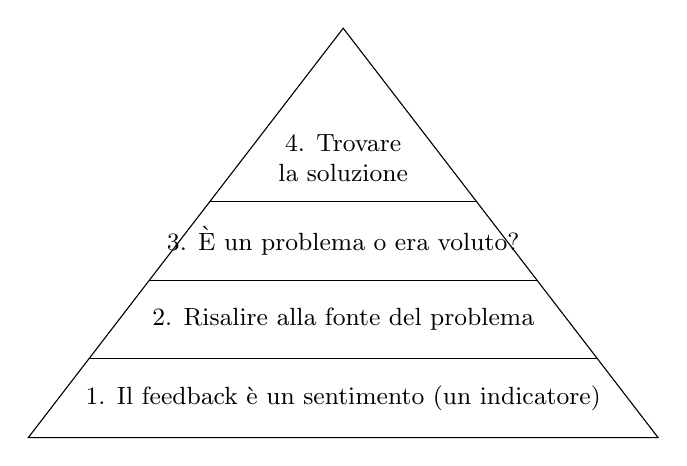
\begin{tikzpicture}[font=\small]
  \draw (0,0) -- (8,0) -- (4,5.2) -- cycle;
  \draw (0.77,1) -- (7.23,1);
  \draw (1.54,2) -- (6.46,2);
  \draw (2.31,3) -- (5.69,3);
  \node at (4,0.5) {1. Il feedback è un sentimento (un indicatore)};
  \node at (4,1.5) {2. Risalire alla fonte del problema};
  \node at (4,2.5) {3. È un problema o era voluto?};
  \node[align=center] at (4,3.55) {4. Trovare\\ la soluzione};
\end{tikzpicture}
\caption{La piramide del feedback come la descrive il relatore: si parte
dalla sensazione riferita da chi dà il feedback e si sale fino alla
soluzione. Ricostruzione schematica; la slide originale non è
disponibile.}
\label{p0:fig:piramide}
\end{figure}

\subsection{I feedback duri}

La piramide è anche un ottimo modo per \textbf{ricevere feedback in modo
professionale}, anche quelli difficili. Il relatore dà spesso feedback
\textbf{duri} ``anche per testarvi'': ``non perché sono stronzo''. Può dire
che una task è ``decente'', e dire anche tutto ciò che è sbagliato;
bisogna ricordarsi di lavorarci sopra e di \textbf{non prenderla sul
personale}. Magari sta testando la reazione, ``perché di fronte al vostro
capo in un'azienda non potete mandarlo a fanculo''.

% ---------------------------------------------------------------------
\section{La tecnica dell'iceberg}
\label{p0:sec:iceberg}

E se il problema è insormontabile? ``Allora, se il problema è
insormontabile, non esiste'', perché il relatore ha imparato la
\textbf{tecnica dell'iceberg} e la racconta ``come mi è stata spiegata''.
Non ha una base scientifica, avverte, ma a livello psicologico lo ha
aiutato molto. È una tecnica di \textbf{categorizzazione dei problemi}: non
è detto che un problema si risolva ``così'', ma la prima cosa da fare quando
lo si affronta è \textbf{descriverlo}, scriverlo in un testo, farne uno
schemino, e cercare di \textbf{classificarlo} in uno di quattro iceberg
(tabella~\ref{p0:tab:iceberg}). Se ne possono anche inventare di nuovi, per
esempio un iceberg ``basso e lungo'', che si estende per molto spazio invece
di essere largo.

\begin{table}[htbp]
\centering
\small
\begin{tabular}{@{}lp{4.4cm}p{5.4cm}@{}}
\toprule
\textbf{Iceberg} & \textbf{Che problema è} & \textbf{Come si affronta} \\
\midrule
\textbf{Alto} & Molto alto, insormontabile se lo si vuole scavalcare. &
Non lo si può prendere di petto: va \textbf{aggirato} in qualche modo. \\
\textbf{Largo} & Semplicemente molto grande, ma poco difficile. & Ci si
mette lì e \textbf{si fa fatica}. \\
\textbf{Nascosto} & Contiene situazioni problematiche, problemi nascosti. &
Obbliga a trovare il \textbf{problema reale} e a risolvere prima quello. \\
\textbf{Mostruoso} & Grande, difficile, complesso. & Richiede un
\textbf{approccio sistematico}, di solito suddividendolo in più parti. \\
\bottomrule
\end{tabular}
\caption{I quattro iceberg della tecnica dell'iceberg, come li presenta il
relatore.}
\label{p0:tab:iceberg}
\end{table}

Perché descrivere un problema con una forma ``geografica'' aiuta? Perché, se
lo si è descritto correttamente, si trova il modo di risolverlo. E, aggiunge
il relatore, la maggior parte delle volte si noterà che
\textbf{suddividere un problema in più parti} è la scelta migliore:
``splittate il problema in più parti, razionalizzate il problema''. Ed è
questo, conclude, il modo per affrontare al meglio il primo anno di AIV, o
tutti e tre.

% ---------------------------------------------------------------------
\section{Le domande finali}
\label{p0:sec:domande}

``Domande? Così recupero.'' E poi, davanti al silenzio: ``Oh, che
cavalcata! No, dai, vi prego, ditemi che avete dei dubbi''.

\subsection{A che cosa serve lo zone out?}

Una studentessa non ha capito il vantaggio dello zone out. Il relatore lo
spiega con la slide di figura~\ref{p0:fig:modi}: lo zone out
\textbf{potenzia la modalità diffusa}, e quindi la possibilità di trovare
soluzioni \emph{out of the box} che non si trovavano perché ci si
focalizzava troppo su un singolo punto. Se la soluzione è ``qui'' e ci si sta
concentrando ``qua'', non ci si arriva; in modalità diffusa il cervello vaga
e a un certo punto impatta nella soluzione. Inoltre rilassa la mente e, così
facendo, attiva il consolidamento, trasformando la working memory in
long-term memory. (Un partecipante commenta che sembra il cervello di un
personaggio di un film d'animazione\footnote{La trascrizione dice ``sembra
il cervello di Infeldo Sghetto 3'': il riferimento non è ricostruibile,
forse \emph{Inside Out}.}; ``vabbè, sì, certo, da qualche parte dovrà pure
venire fuori''.)

\subsection{La soluzione arriva sotto la doccia: e poi?}

Gabriele chiede: se finisco la giornata di lavoro con un problema aperto e
la soluzione mi viene a casa, sotto la doccia, mi rimetto a lavorare o me la
tengo per il giorno dopo? Nessuna delle due: \textbf{ci si prendono degli
appunti}. La tecnica migliore è avere sempre con sé un taccuino o il
cellulare (``non si dovrebbe fare, meglio un taccuino''). Il relatore tiene
il cellulare sul comodino: a volte, di notte, tornando dal bagno, gli viene
in mente qualcosa e se lo segna; a volte, fuori con il cane, si registra
mentre parla, e a volte si sblocca proprio parlando.

Tutto ciò che si è visto oggi, aggiunge, verrà ripreso durante il primo
anno, ma sono concetti che ``precedono il corso stesso'': durante l'anno non
c'è tempo, si fa il proprio corso. Qualcosa di neurocognitività tornerà a
narrative design e, al secondo anno, a game design, perché aiuta moltissimo
a \textbf{mappare il cervello del giocatore}, a capire come stimolarne certe
reazioni. Sarebbe bello approfondire, ma ``un po' rimane anche a voi'':
prendere le slide, approfondirle, leggerle.

\subsection{Arrivare da un'altra accademia}

Gabriele comincia direttamente dal secondo anno, avendo già fatto un anno in
un'altra accademia (``che purtroppo poi si sa com'è andata''); teme di
trovarsi spaesato non tanto per gli argomenti quanto per il metodo. Il
relatore distingue: \textbf{il metodo di studio è dello studente}; è il
\textbf{metodo di insegnamento} a essere diverso, e lo è (``senza nulla
togliere ai colleghi''): c'è un motivo per cui AIV fa nove ore di lezione a
settimana e il resto lo lascia allo studente. I consigli:
\begin{itemize}
  \item affrontare l'anno con \textbf{mentalità aperta}, senza crearsi
        pregiudizi solo perché arrivano cose diverse da quelle a cui si è
        abituati (e vale per tutti);
  \item se qualcosa non torna con l'istruzione precedente, \textbf{fare
        domande}, anche provocatorie: il relatore adora quando uno studente
        gli dice ``prof, questa cosa del viaggio dell'eroe io non la
        condivido, parliamone'' (``non vedo l'ora, davvero''), ``perché si
        apprende meglio''; avrebbe un problema se, da non professionista, si
        rifiutasse di rispondere per paura di come rispondere;
  \item ricordare che non è il metodo di insegnamento a cambiare lo
        studente: è il suo metodo di studio, ed è l'argomento ciò che si
        impara davvero, non il modo (``poi il modo aiuta molto, me ne rendo
        conto'').
\end{itemize}
Il problema vero, prevede il relatore, non sarà il metodo, ma il fatto che i
compagni hanno già un anno alle spalle e hanno affrontato cose che Gabriele
non ha visto, e su cui dovrà aggiornarsi. Il consiglio ``spassionato'':
\textbf{fare amicizia, aprirsi agli altri}. Ci si può far male, ``fa parte
del gioco''; ma essere aperti non vuol dire ``dare la propria password a
tutti'' (``a volte gli studenti mi prendono troppo alla lettera''): vuol
dire \textbf{dialogare}, e dialogare ``batte qualsiasi cosa''. Creare una
buona sinergia con la classe, cercando compromessi se serve.

\subsection{Come accorgersi di stare imparando un metodo sbagliato?}

Federico chiede come ci si accorge di stare imparando un metodo sbagliato,
per evitare il ``polso del chitarrista''. In parte sono i docenti a dirlo,
con i feedback: certe cose lo studente non può capirle da solo. Altre invece
le si nota confrontandosi con i compagni: ``cavolo, ma a me questa cosa
viene difficile, perché?''; ``mi viene, ma la sento macchinosa,
arzigogolata''. È possibile, non certo, che si stia avviando un effetto
Einstellung: si sta forse aprendo la bottiglia con una forza esercitatissima,
quando ne servirebbe molta meno.

\subsection{E all'università?}

Filippo, che frequenta anche l'università, chiede se questi metodi si
applichino a contesti più teorici, con meno possibilità di cambiare medium.
Il relatore premette di parlare ``con le pinze''. Ha fatto l'università e
``se ne pente parzialmente'': secondo lui l'università italiana ha
``tantissime competenze e conoscenze, ma pessime metodologie di
preparazione''; è soprattutto un istituto di ricerca e di studio, tranne le
facoltà pragmatiche (suo fratello è ingegnere elettrotecnico, con dottorato,
e doveva letteralmente fare circuiti; medicina è molto pratica). Ci sono
università di game design in Italia, ma con limiti: il ministero impone
esami come storia del videogioco, ``che è molto utile, ovviamente''.

Lui lavora per lo più con clienti, e al cliente non interessa la teoria né la
storia del videogioco fine a se stessa. La storia è utile \textbf{quando la si
applica}. Esempio, ripreso da ``stamattina'': il fatto che \emph{Pac-Man}
rallenti impercettibilmente mangiando i pallini\footnote{Si veda il
capitolo sul narrative design (sezione~\ref{p3:sec:mindset}). Il dettaglio
storico è che Pac-Man si ferma per un fotogramma a ogni pallino mangiato,
risultando un po' più lento dei fantasmi nei corridoi pieni di pallini.}
serve se un giorno, al lavoro, bisogna far rallentare il personaggio, senza
che il giocatore se ne accorga, quando fa certi passi, per renderlo più
raggiungibile e dargli la sensazione di ``oddio, non ce la faccio!'', magari
in una scena molto tesa di un horror: si prende la soluzione di Pac-Man e la
si adegua al contesto.

È molto importante che esista la ricerca: AIV ha bisogno degli studiosi,
il relatore lavora spesso con consulenti esperti di antropologia o di
storia. Ma non crede che un neolaureato sia pronto per l'industria, perché
molte tecniche della game industry non si insegnano all'università e
viceversa. Cita, senza nominarlo, uno studioso americano diventato un
professore importantissimo, che pubblica saggi di game design: saggi che
mostrano non un'incapacità di comprendere i framework, ma una comprensione
``in una scatola chiusa'', perché non li ha mai visti all'opera in un gioco.
È la differenza fra imparare a riparare un motore e fare davvero il
meccanico, quando le cose non sono uno a uno e vanno adattate.

Filippo precisa che la sua fatica all'università è data proprio dal ciclo
``testo, esame'', senza pratica, discussione e comunicazione. Il relatore
ribadisce che in AIV, in game design, tutte le task sono pratiche: al primo
anno su prodotti pubblicati (l'analisi del \emph{core loop} di un gioco, per
dire). All'università ci sono limiti: l'ultima volta che ha collaborato con
un ateneo gli hanno detto che il ministero impone un tetto del 30\% alle
attività di laboratorio. A lui il ciclo ``studio, studio, esame'' non
piace, perché nella vita reale non funziona così: ``il mio esame è la
pubblicazione'', che arriva dopo tre, quattro, cinque anni. Le conoscenze
generali che dà l'università sono ``imprescindibili ed enormi'', ma si
possono anche recuperare. Fa l'esempio della dizione nel doppiaggio: le
regole si assorbono, e al direttore interessa che la battuta sia detta bene;
e a volte, soprattutto gli americani, chiedono uno slang, e ``prova a
chiedere in università di farti imparare lo slang newyorkese di un
rapper''\footnote{La trascrizione dice ``addizione'' per ``dizione''. Il
passaggio è confuso, ma il senso è che certe competenze professionali si
apprendono sul campo, da altri professionisti, più che in università.}: gli
attori americani si formano facendo esperienza, andando da altri attori.

Non vuole criticare l'università: collabora con università e la rispetta. Ma
non gli piacciono quelli che, finito un corso universitario, pensano di
uscire e andare dritti a fare videogiochi. ``Io l'ho sentito sulla mia
pelle'': uscito dall'università non trovava lavoro e non capiva perché;
dieci anni dopo l'ha capito: quelle cose non le sapeva, e ha dovuto
``abbassare la cresta, fare un lavoro di umiltà e dire: ho studiato
altro''.

\subsection{Anatomia, per chi l'ha già studiata}

Una studentessa ha visto che al primo anno c'è anatomia e, avendo già fatto
tre esami di anatomia, chiede come sarà strutturato il corso. Va chiesto al
direttore di 3D art, nell'incontro dedicato (capitolo~\ref{p6:cap:3d}): il
relatore sa poco di quel corso, se non che al primo anno ci sarà una
collaborazione con i narrative per il \emph{world building} di un
gioco\footnote{Nella trascrizione: ``per il war building del giocato'',
probabilmente ``del giocattolo'': il corso di narrative prevede un modulo
di world building per i giocattoli (si veda il capitolo~\ref{p3:cap:narrative}).};
``vi diremo tutto a tempo debito'', in primavera.

\subsection{Le fiere: chi paga?}

Ultima domanda: se uno degli eventi di settore richiesti per il certificato
di eccellenza (sezione~\ref{p1:sec:eccellenza}) fosse una fiera come la
Gamescom, le spese sarebbero individuali? AIV fornisce \textbf{il biglietto
e l'alloggio} (dopo un'incertezza: ``vitto e alloggio\ldots\ scusatemi,
biglietto. No, alloggio'') ma non il trasporto, per \textbf{una fiera
all'anno}, a chi ha acquistato l'opzione \emph{Experience}; ``c'è scritto
sul sito''. La fiera la decide AIV ogni anno, sulla base di quella più
indicata; al terzo anno è al cento per cento la \textbf{First
Playable}\footnote{La trascrizione dice ``force playable''. La First
Playable è l'evento business dell'industria videoludica italiana che si
tiene a Firenze.}, ``perché alla First Playable bisogna andare''. A volte
le fiere mandano sconti, e la segreteria li comunica su Discord:
``sfruttateli assolutamente''. Ma AIV non ha la forza economica di mandare
tutti in fiera, solo chi ha l'Experience. Il relatore, che è di Milano, alla
Milan Games Week di solito scrive un messaggio per organizzare un
\emph{meet up}. La Gamescom è ``estremamente costosa'' anche da soli: chi
vuole andarci con AIV deve avere l'Experience, altrimenti si paga biglietto
e albergo. E la fiera, ogni anno, cambia.
